\def\V{2.05}
\def\docexdir{docs/}
%THE LINES ABOVE MUST BE THE FIRST LINES. THEY WILL BE AUTOMATICALLY MODIFIED
%TO THE CURRENT VERSION / DOC DIRECTORY OF PROVERIF


\documentclass{book}

\usepackage[utf8]{inputenc}
\usepackage{amsmath}
\usepackage[a4paper,hmargin=1in,vmargin=1.25in]{geometry}
\usepackage[allowmove]{url}

%\usepackage{pstricks}
\usepackage{amsfonts}
\usepackage{verbatim,upquote}
\usepackage{listings}\lstset{language=ProVerif,numbers=left,tabsize=2,showlines=true,mathescape=true}
\usepackage{graphicx}
\usepackage{hyperref}

\usepackage{ulem}\normalem
\usepackage{authblk}
%\usepackage{appliedpi}
\newcommand{\nill}{0}

\usepackage{color}

\usepackage{float}
\floatstyle{ruled}\restylefloat{figure}

\usepackage{tikz}
\usetikzlibrary{fit}
\usetikzlibrary{shapes.geometric}

\newcommand{\nonterm}[1]{\langle\mathit{#1}\rangle}
\newcommand{\filenamevar}{\nonterm{filename}}
\newcommand{\switchdir}{\nonterm{switch}}
\newcommand{\opamsubdir}[1]{\nolinkurl{~/.opam/}$\switchdir$\nolinkurl{/#1}}

\newcommand{\tblue}[1]{\textcolor{blue}{REMARK: \emph{#1}}}

\renewcommand{\marginpar}[1]{\tblue{#1}}
%\renewcommand{\sout}[1]{}



\newcommand{\A}{A}
\newcommand{\B}{B}
\newcommand{\M}{I}
\newcommand{\T}{S}

\newcommand{\seq}[1]{\textrm{seq}\nonterm{#1}}
\newcommand{\neseq}[1]{\textrm{seq}^+\nonterm{#1}}

\title{ProVerif \V:\\
Automatic Cryptographic Protocol Verifier,\\
User Manual and Tutorial}

\author{Bruno Blanchet, Ben Smyth, Vincent Cheval, and Marc Sylvestre}

\date{\vskip -0.5cm \url{Bruno.Blanchet@inria.fr}, \url{research@bensmyth.com},
\url{vincent.cheval@inria.fr}, \url{marc.sylvestre@inria.fr}\\[0.75cm] \today}

\begin{document}


\frontmatter                %Get rid of title on second page if blank - i.e. \thispagestyle{empty}
\pagenumbering{roman}
\maketitle

\chapter*{Acknowledgements}

This manual was written with support from the Direction G{\'e}n{\'e}rale pour l'Armement (DGA)
and the EPSRC project \emph{UbiVal} (EP/D076625/2).
ProVerif was developed while Bruno Blanchet was affiliated with Inria and with CNRS, Ecole Normale Supérieure, Paris, Vincent Cheval was affiliated with CNRS and Inria, and Marc Sylvestre was affiliated with Inria. This manual was written while Bruno Blanchet was affiliated with Inria and with CNRS, Ecole Normale Supérieure, Paris,  Ben Smyth was affiliated with Ecole Normale Supérieure, Paris and with University of Birmingham, Vincent Cheval was affiliated with CNRS and Inria, and Marc Sylvestre was affiliated with Inria.
The development of ProVerif would not have been possible without the helpful remarks from the research community; their contributions are greatly appreciated and further feedback is encouraged.

%DONE \marginpar{Update the extraction procedure if I make a separate package for documentation; update the distrib scripts of ProVerif to build the documentation automatically with the correct ProVerif version number and directory for doc examples}
%List of files that must be provided in the doc distribution
% hello.pv, hello_ext.pv, hello_var.pv,
% ex_handshake.pv, ex\_handshake\_annotated.pv, ex\_handshake\_annotated\_fixed.pv, ex\_handshake\_forward\_secrecy\_skB.pv, ex\_handshake\_RoR.pv
% ex\_noninterf1.pv, ex\_noninterf2.pv, ex\_weaksecret.pv, dh-fs.pv
% NeedhamSchroederPK-var1.pv, NeedhamSchroederPK-var2.pv, NeedhamSchroederPK-var3.pv, NeedhamSchroederPK-corr-mutual-auth.pv, NeedhamSchroederPK-corr-ake.pv, NeedhamSchroederPK-corr-ake-RoR.pv, NeedhamSchroederPK-corr-all-messages.pv
% ex\_predicates.pv

%DO NOT PROVIDE NeedhamSchroederPK-var1.processes.pv, bestmodel.pv, eq.pv, reduc.pv
%I WILL PROVIDE THE PDF OF THE MANUAL + ALL .pv examples except NeedhamSchroederPK-var1.processes.pv, bestmodel.pv, eq.pv, reduc.pv

\tableofcontents
\listoffigures
%\listoftables

\mainmatter

%%%%%%%%%%%%%%%%%%%%%%%%%%%%%%%%%%%%%%%%%%%%%%%%%%%%%%%%%%%%%%%%%%%%%%%
%%%%%%%%%%%%%%%%%%%%%%%%%%%%%%%%%%%%%%%%%%%%%%%%%%%%%%%%%%%%%%%%%%%%%%%
%%%%%%%%%%%%%%%%%%%%%%%%%%%%%%%%%%%%%%%%%%%%%%%%%%%%%%%%%%%%%%%%%%%%%%%

\chapter{Introduction}

This manual describes the ProVerif software package version \V. ProVerif is a tool for automatically analyzing the security of cryptographic protocols. Support is provided for, but not limited to, cryptographic primitives including: symmetric and asymmetric encryption; digital signatures; hash functions; bit-commitment; and non-interactive zero-knowledge proofs. ProVerif is capable of proving reachability properties, correspondence assertions, and observational equivalence. These capabilities are particularly useful to the computer security domain since they permit the analysis of secrecy and authentication properties. Moreover, emerging properties such as privacy, traceability, and verifiability can also be considered. Protocol analysis is considered with respect to an unbounded number of sessions and an unbounded message space. Moreover, the tool is capable of attack reconstruction: when a property cannot be proved, ProVerif tries to reconstruct an execution trace that falsifies the desired property.

\section{Applications of ProVerif}\label{sec:applications}

The applicability of ProVerif has been widely demonstrated. Protocols from the literature have been successfully analyzed: flawed and corrected versions of Needham-Schroeder public-key~\cite{Needham78,Lowe96} and shared key~\cite{Needham78,Burrows89,Needham87}; Woo-Lam public-key~\cite{Woo92,Woo97} and shared-key~\cite{Woo92,Anderson95,Abadi96,Woo97,Gordon2003}; Denning-Sacco~\cite{Denning81,Abadi96}; Yahalom~\cite{Burrows89}; Otway-Rees~\cite{Otway87,Abadi96,Paulson98}; and Skeme~\cite{Krawczyk96}.
%ProVerif has also been able to prove strong secrecy~\cite{Blanchet04,Abadi99c,Cortier06c} in: the corrected version of Needham-Schroeder public-key~\cite{Lowe96}; Otway-Rees~\cite{Otway87}; Yahalom~\cite{Burrows89}; and Skeme~\cite{Krawczyk96}.
The resistance to password guessing attacks has been demonstrated for the password-based protocols EKE~\cite{Bellovin92} and Augmented EKE~\cite{Bellovin93}.

ProVerif has also been used in more substantial case studies:
%
\begin{itemize}
	\item{Abadi \& Blanchet~\cite{Abadi04f}} use correspondence assertions to verify the certified email protocol~\cite{Abadi02b}.

	\item{Abadi, Blanchet \& Fournet~\cite{Abadi07}} analyze the JFK (Just Fast Keying)~\cite{Aiello:2004:JFK} protocol, which was one of the candidates to replace IKE as the key exchange protocol in IPSec, by combining manual proofs with ProVerif proofs of correspondences and equivalences.

	\item{Blanchet \& Chaudhuri~\cite{Blanchet08b}} study the integrity of the Plutus file system~\cite{Kallahalla03} on untrusted storage, using correspondence assertions, resulting in the discovery, and subsequent fixing, of weaknesses in the initial system.

	\item{Bhargavan \emph{et al.}~\cite{Bhargavan06,Bhargavan06b,Bhargavan08}} use ProVerif to analyze cryptographic protocol implementations written in F\#; in particular, the Transport Layer Security (TLS) protocol has been studied in this manner~\cite{Bhargavan08b}.

	\item{Chen \& Ryan~\cite{ChenRyan:FAST09}} evaluate authentication protocols found in the Trusted Platform Module (TPM), a widely deployed hardware chip, and discovered vulnerabilities.

	\item{Delaune, Kremer \& Ryan~\cite{DKR09,Kremer05} and Backes, Hritcu \& Maffei~\cite{Backes08a}} formalize and analyze privacy properties for electronic voting using observational equivalence.

	\item{Delaune, Ryan \& Smyth~\cite{DRS08} and Backes, Maffei \& Unruh~\cite{Backes07c}} analyze the anonymity properties of the trusted computing scheme Direct Anonymous Attestation (DAA)~\cite{BCC04,SRC07} using observational equivalence.

	\item{K\"{u}sters \& Truderung~\cite{Kuesters09,Kuesters08b}} examine protocols with Diffie-Hellman exponentiation and XOR.

	\item{Smyth, Ryan, Kremer \& Kourjieh~\cite{SRKK10,SRK10}} formalize and analyze verifiability properties for electronic voting using reachability.
        \item Bhargavan, Blanchet and Kobeissi verify Signal~\cite{KobeissiEuroSP17} and TLS 1.3~\cite{BhargavanSP17}.

\item Blanchet verifies the ARINC 823 avionic protocols~\cite{Blanchet17}.
\end{itemize}
%
For further examples, please refer to: \url{http://proverif.inria.fr/proverif-users.html}.

\section{Scope of this manual}

This manual provides an introductory description of the ProVerif software package version \V. The remainder of this chapter covers software support (Section~\ref{sec:support}) and installation (Section~\ref{sec:install}). Chapter~\ref{chap:basic} provides an introduction to ProVerif aimed at new users, advanced users may skip this chapter without loss of continuity. Chapter~\ref{sec:.pv} demonstrates the basic use of ProVerif. Chapter~\ref{sec:advLang} provides a more complete coverage of the features of ProVerif. Chapter~\ref{sec:caseStudy} demonstrates the applicability of ProVerif with a case study. Chapter~\ref{sec:advTheory} considers advanced topics and Chapter~\ref{sec:outlook} concludes.
%
For reference, the complete grammar of ProVerif is presented in Appendix~\ref{app:grammar}.
This manual does not attempt to describe the theoretical foundations of the internal algorithms used by ProVerif since these are available elsewhere (see Chapter~\ref{sec:outlook} for references); nor is the applied pi calculus \cite{Abadi2001, Smyth2010, AbadiBlanchetFournetJACM17}, which provides the basis for ProVerif, discussed.

\section{Support}\label{sec:support}

Software bugs and comments should be reported by e-mail to:
\begin{center}
	\url{proverif-dev@inria.fr}
\end{center}
User support, general discussion and new release announcements are provided by the ProVerif mailing list. To subscribe to the list, send an email to \url{sympa@inria.fr} with the subject ``subscribe proverif'' (without quotes). To post on the list, send an email to:
\begin{center}
	\url{proverif@inria.fr}
\end{center}
Non-members are not permitted to send messages to the mailing list.

\section{Installation}\label{sec:install}

ProVerif is compatible with the Linux, Mac, and Windows operating systems;
it can be downloaded from:
\begin{center}
	\url{http://proverif.inria.fr/}
\end{center}
The remainder of this section covers installation on Linux, Mac, and Windows platforms.

\subsection{Installation via OPAM}

ProVerif has been developed using Objective Caml (OCaml) and OPAM is
the package manager of OCaml. Installing via OPAM is the simplest,
especially if you already have OPAM installed.
\begin{enumerate}

\item If you do not already have OPAM installed, download it from
\begin{quote}
	\url{https://opam.ocaml.org/}
\end{quote}
and install it.

\item If you already have OPAM installed, run
\begin{quote}
\texttt{opam update}
\end{quote}
to make sure that you get the latest version of ProVerif.

\item Run
\begin{quote}
\texttt{opam depext conf-graphviz}\\
\texttt{opam depext proverif}\\
\texttt{opam install proverif}
\end{quote}
The first line installs graphviz, if you do not already have it. You may also install it using the package manager of your Linux, OSX, or cygwin distribution, especially if opam fails to install it. It is needed only for the graphical display of attacks.

The second line installs GTK+2 including development libraries, if you do not already have it. You may also install it using the package manager of your distribution.  You may additionally need to install \texttt{pkgconfig} using the package manager of your distribution, if you do not already have it and it is not installed by \texttt{opam depext proverif}. (This happens in particular on some OSX installations.) GTK+2 is needed for the interactive simulator \texttt{proverif\_interact}.

The third line installs ProVerif itself and its OCaml dependencies. ProVerif executables are in
\opamsubdir{bin}, which is in the {\tt PATH},
examples are in \opamsubdir{doc/proverif},
and various helper files are in \opamsubdir{share/proverif}.
The directory $\switchdir$ is the opam switch in which you installed
ProVerif, by default \texttt{system}.

\item Download the documentation package \texttt{proverifdoc\V.tar.gz}
from
\begin{quote}
	\url{http://proverif.inria.fr/}
\end{quote}
and uncompress it (e.g. using \texttt{tar -xzf proverifdoc\V.tar.gz} or using
your favorite file archive tool). That gives you the manual and a few additional
examples.

\end{enumerate}

\subsection{Installation from sources (Linux/Mac/cygwin)}

\begin{enumerate}

\item On Mac OS X, you need to install XCode if you do not
already have it. It can be downloaded from \url{https://developer.apple.com/xcode/}.

\item ProVerif has been developed using Objective Caml (OCaml), accordingly OCaml version 4.03 or higher is a prerequisite to installation and can be downloaded from \url{http://ocaml.org/}, or installed via the package manager of your distribution. OCaml provides a byte-code compiler (\texttt{ocamlc}) and a native-code compiler (\texttt{ocamlopt}). Although ProVerif does not strictly require the native-code compiler, it is highly recommended to achieve large performance gains.

\item The installation of graphviz is required if you want to have a graphical representation of the attacks that ProVerif might find. Graphviz can be downloaded from \url{http://graphviz.org} or installed via the package manager of your distribution.

\item The installation GTK+2.24 and LablGTK2 is required if you want to
run the interactive simulator \texttt{proverif\_interact}. Use the
package manager of your distribution to install GTK+2 including its
development libraries if you do not already have it and
download \texttt{lablgtk-2.18.6.tar.gz} from
\begin{quote}
	\url{http://lablgtk.forge.ocamlcore.org/}
\end{quote}
and follow the installation instructions in their README file.

\sloppy

\item Download the source package \texttt{proverif\V.tar.gz} and the documentation
package \texttt{proverifdoc\V.tar.gz}
from
\begin{quote}
	\url{http://proverif.inria.fr/}
\end{quote}

\fussy

	\item Decompress the archives:
	\begin{enumerate}
		\item using GNU tar
		\begin{quote}
			\texttt{tar -xzf proverif\V.tar.gz}\\
			\texttt{tar -xzf proverifdoc\V.tar.gz}
		\end{quote}
		\item using tar
		\begin{quote}
			\texttt{gunzip proverif\V.tar.gz} \\
			\texttt{tar -xf proverif\V.tar}\\
			\texttt{gunzip proverifdoc\V.tar.gz} \\
			\texttt{tar -xf proverifdoc\V.tar}
		\end{quote}
	\end{enumerate}
	This will create a directory \texttt{proverif\V} in the current directory.

	\item You are now ready to build ProVerif:
	\begin{quote}
		\texttt{cd proverif\V} \\
		\texttt{./build}
	\end{quote}
        (If you did not install LablGTK2, the compilation of
        \texttt{proverif\_interact} fails, but the executables
        \texttt{proverif} and \texttt{proveriftotex} are still
        produced correctly, so you can use ProVerif normally, but cannot
        run the interactive simulator.)

	\item ProVerif has now been successfully installed.
\end{enumerate}

\subsection{Installation from binaries (Windows)}

Windows users may install ProVerif using the binary distribution, as described below. They may also install cygwin and install ProVerif from sources as explained in the previous section.

%\paragraph{From binary}

\begin{enumerate}
\item The installation of graphviz is required if you want to have a graphical representation of the attacks that ProVerif might find. Graphviz can be downloaded from \url{https://graphviz.gitlab.io/_pages/Download/Download_windows.html}.
Make sure that the \texttt{bin} subdirectory of the Graphviz installation directory is in your PATH.

\sloppy

\item The installation GTK+2.24 is required if you want to run the interactive
simulator \texttt{proverif\_interact}. At
	\begin{quote}
        \url{https://download.gnome.org/binaries/win32/gtk\%2B/2.24/}
%	\url{ftp://ftp.gnome.org/pub/gnome/binaries/win32/gtk+/2.24/}
	\end{quote}
download \nolinkurl{gtk+-bundle_2.24.10-20120208_win32.zip},
unzip it in the directory \nolinkurl{C:\\GTK}, and add \nolinkurl{C:\\GTK\\bin} to your PATH.

\item Download the Windows binary package \texttt{proverifbin\V.tar.gz} and the documentation
package \texttt{proverifdoc\V.tar.gz}
from
\begin{quote}
	\url{http://proverif.inria.fr/}
\end{quote}

\fussy

	\item Decompress the \texttt{proverifbin\V.tar.gz} and \texttt{proverifdoc\V.tar.gz} archives in the same directory using your favorite file archive tool (e.g. WinZip).

	\item ProVerif has now been successfully installed in the directory where the file was extracted.
\end{enumerate}


%% \paragraph{From source}

%% \begin{enumerate}

%% \item ProVerif has been developed using Objective Caml (OCaml), accordingly OCaml version 4.03 or higher is a prerequisite to installation and can be downloaded from \url{http://ocaml.org/}.

%% \item The installation of graphviz is required if you want to have a graphical representation of the attacks that ProVerif might find. Graphviz can be downloaded from \url{http://graphviz.org}.

%% \sloppy

%% \item Download the source package \texttt{proverif\V.tar.gz} and the documentation
%% package \texttt{proverifdoc\V.tar.gz}
%% from
%% \begin{quote}
%% 	\url{http://proverif.inria.fr/}
%% \end{quote}

%% \fussy

%% 	\item Decompress the \texttt{proverif\V.tar.gz} and \texttt{proverifdoc\V.tar.gz} archives in the same directory using your favorite file archive tool (e.g. WinZip).
%% 	\item Open a command shell and change to the directory where the file was extracted.
%% 	\item You are now ready to build ProVerif:
%% 	\begin{quote}
%% 		\texttt{./build.bat}
%% 	\end{quote}
%% 	\item ProVerif has now been successfully installed.
%% \end{enumerate}
%% Note: this installation procedure, using the \texttt{build.bat} script,
%% relies on the OCaml bytecode compiler, which works in all Windows
%% installations, but produces slower executables than the native code compiler.
%% This installation procedure does not produce the simulator \texttt{proverif\_interact}.
%% If you have installed cygwin and want to install from source,
%% you should rather use the Linux/Mac installation procedure, which allows
%% you to use the OCaml native code compiler and produce the simulator \texttt{proverif\_interact}.

\subsection{Emacs}

If you use the emacs text editor for editing ProVerif input
files, you can install the emacs mode provided with the ProVerif distribution.
\begin{enumerate}

\item Copy the file \texttt{emacs/proverif.el} (if you installed by OPAM
in the switch $\switchdir$, the file \opamsubdir{share/proverif/emacs/proverif.el})
to a directory where Emacs will find it
(that is, in your emacs load-path).

\item Add the following lines to your \texttt{.emacs} file:
\begin{verbatim}
(setq auto-mode-alist
       (cons '("\\.horn$" . proverif-horn-mode)
       (cons '("\\.horntype$" . proverif-horntype-mode)
       (cons '("\\.pv[l]?$" . proverif-pv-mode)
       (cons '("\\.pi$" . proverif-pi-mode) auto-mode-alist)))))
(autoload 'proverif-pv-mode "proverif" "Major mode for editing ProVerif code." t)
(autoload 'proverif-pi-mode "proverif" "Major mode for editing ProVerif code." t)
(autoload 'proverif-horn-mode "proverif" "Major mode for editing ProVerif code." t)
(autoload 'proverif-horntype-mode "proverif" "Major mode for editing ProVerif code." t)
\end{verbatim}
\end{enumerate}

%% \subsection{Atom}

%% There is also a ProVerif mode for the text editor Atom (\url{https://atom.io/}), by
%% Vincent Cheval.
%% It can be downloaded from the Atom web site; the package name is \texttt{language-proverif}.

\section{Copyright}

The ProVerif software is distributed under the GNU general public license. For details see:
%
\begin{center}
	\url{http://proverif.inria.fr/LICENSE}
\end{center}

%%%%%%%%%%%%%%%%%%%%%%%%%%%%%%%%%%%%%%%%%%%%%%%%%%%%%%%%%%%%%%%%%%%%%%%
%%%%%%%%%%%%%%%%%%%%%%%%%%%%%%%%%%%%%%%%%%%%%%%%%%%%%%%%%%%%%%%%%%%%%%%
%%%%%%%%%%%%%%%%%%%%%%%%%%%%%%%%%%%%%%%%%%%%%%%%%%%%%%%%%%%%%%%%%%%%%%%


\chapter{Getting started}\label{chap:basic}

This chapter provides a basic introduction to ProVerif and is aimed at new users; experienced users may choose to skip this chapter. ProVerif is a command-line tool which can be executed using the syntax:
\begin{quote}
	\texttt{./proverif} \texttt{[options]} $\filenamevar$
\end{quote}
where \texttt{./proverif} is ProVerif's binary; $\filenamevar$ is the input file; and command-line parameters \texttt{[options]} will be discussed later (Section~\ref{sec:command-line}). ProVerif can handle input files encoded in several languages. The typed pi calculus is currently considered to be state-of-the-art and files of this sort are denoted by the file extension $\texttt{.pv}$.
This manual will focus on protocols encoded in the typed pi calculus.
(For the interested reader, other input formats are mentioned in Section~\ref{sec:altLang} and in {\tt docs/manual-untyped.pdf}.)
The pi calculus is designed for representing concurrent processes that interact using communications channels such as the Internet.
%These channels may be public, for example, the Internet; or private, for example, face-to-face communication.

ProVerif is capable of proving reachability properties, correspondence assertions, and observational equivalence. This chapter will demonstrate the use of reachability properties and  correspondence assertions in a very basic manner. The true power of ProVerif will be discussed in the remainder of this manual.

% \paragraph{ProVerif Editor.} New users may be interested in the ProVerif editor which was developed by Joeri de Ruiter in Python to provide an integrated development environment for ProVerif. The tool is available for download from the following URL:
% %
% \begin{center}
% 	\url{http://sourceforge.net/projects/proverifeditor/}
% \end{center}
%%% Cut because it does not support the typed front-end

\paragraph{Reachability properties.} Let us consider the ProVerif script:
%
\lstinputlisting[linerange={1-6,9}]{examples/hello.pv}
%
%Reverted to listings version 1.3 to solve this problem!
%\marginpar{The listing package seems to have changed its line numbering...}
Line~1 contains the comment \emph{``hello.pv: Hello World Script''}; comments are enclosed by \lstinline!(* comment *)!. Line~3 declares the \emph{free name} \lstinline!c! of type \lstinline!channel! which will later be used for public channel communication. Lines~5 and 6 declare the free names \lstinline!Cocks! and \lstinline!RSA! of type \lstinline!bitstring!, the keyword \lstinline![private]! excludes the names from the attacker's knowledge. Line 10 declares the start of the \emph{main} process. Line~11 outputs the name \lstinline!RSA! on the \emph{channel} \lstinline!c!. Finally, the termination of the process is denoted by \lstinline!0! on Line~12.

%Formally, names are modeled as freshly computed random values.
Names may be of any type, but we explicitly distinguish names of type \lstinline!channel! from other types, since the former may be used as a communications channel for message input/output. The concept of bound and free names is similar to local and global scope in programming languages; that is, free names are globally known, whereas bound names are local to a process. By default, free names are known by the attacker. Free names that are not known by the attacker must be declared \emph{private} with the addition of the keyword \lstinline![private]!. The message output on Line~11 is broadcast using a \emph{public channel} because the channel name \lstinline!c! is a free name; whereas, if \lstinline!c! were a bound name or explicitly excluded from the attacker's knowledge, then the communication would be on a \emph{private channel}. For convenience, the final line may be omitted and hence \lstinline!out(c,RSA)! is an abbreviation of \lstinline!out(c,RSA);0!.

Properties of the aforementioned script can be examined using ProVerif. For example, to test as to whether the names \lstinline!Cocks! and \lstinline!RSA! are available derivable by the attacker, the following lines can be included before the main process:
%
\lstinputlisting[linerange={7-8}]{examples/hello.pv}
%
Internally, ProVerif attempts to prove that a state in which the names \lstinline!Cocks! and \lstinline!RSA! are known to the attacker is unreachable (that is, it tests the queries \lstinline!not attacker(RSA)! and \lstinline!not attacker(Cocks)!, and these queries are true when the names are \emph{not} derivable by the attacker). This makes ProVerif suitable for proving the secrecy of terms in a protocol.

Executing ProVerif (\texttt{./proverif {\docexdir}hello.pv}) produces the output:
%
\verbatiminput{examples/hello.pv.out}
%
As can be interpreted from \verb!RESULT not attacker:(Cocks[]) is true!, the attacker has not been able to obtain the free name \lstinline!Cocks!. The attacker has, however, been able to obtain the free name \lstinline!RSA! as denoted by the \verb!RESULT not attacker:(RSA[]) is false.! ProVerif is also able to provide an attack trace. In this instance, the trace is very short and denoted by
\begin{verbatim}
out(c, ~M) with ~M = RSA at {1}

The attacker has the message ~M = RSA.
\end{verbatim}
which means that the name \lstinline!RSA! is output on channel \lstinline!c! at \emph{point \{1\}} in the process and stored by the attacker in \verb!~M!, where point \lstinline!{1}! is annotated on Line~2 of the output. ProVerif concludes the trace by saying that the attacker has \lstinline!RSA!. ProVerif also provides an English language description of the \emph{derivation} denoted by
\begin{verbatim}
1. The message RSA[] may be sent to the attacker at output {1}.
attacker(RSA[]).

2. By 1, attacker(RSA[]).
The goal is reached, represented in the following fact:
attacker(RSA[]).
\end{verbatim}
A derivation is the ProVerif internal representation of how the attacker may break the desired property, here may obtain \lstinline!RSA!. It generally corresponds to an attack as in the example above, but may sometimes correspond to a false attack because of the internal approximations made by ProVerif. In contrast, when ProVerif presents a trace, it always corresponds to a real attack. See Section~\ref{sec:output} for more details.
The output ends with a summary of the results for all queries.

\paragraph{Correspondence assertions.} Let us now consider an extended variant \texttt{{\docexdir}hello\_ext.pv} of the script:
%
\lstinputlisting{examples/hello_ext.pv}
%
Lines~1-7 should be familiar. Lines~8-9 declare events \lstinline!evCocks! and \lstinline!evRSA!. Intuition suggests that Line~11 is some form of query. Lines~13-14 should again be standard. Line~15 contains a message input  of type \lstinline!bitstring! on channel \lstinline{c} which it binds to the variable \lstinline!x!. Lines~16-20 denote an if-then-else statement; the body of the then branch can be found on Lines~17-18 and the else branch on Line~20. We remark that the code presented is a shorthand for the more verbose
\begin{lstlisting}[numbers=none]
if x = Cocks then event evCocks;event evRSA;0 else event evRSA;0
\end{lstlisting}
where \lstinline!0! denotes the end of a branch (termination of a process). The statement \lstinline!event evCocks! (similarly \lstinline!event evRSA!) declares an event and the query
\begin{lstlisting}[numbers=none]
query event(evCocks) ==> event(evRSA)
\end{lstlisting}
is true if and only if, for all executions of the protocol, if the event \lstinline!evCocks! has been executed, then the event \lstinline!evRSA! has also been executed before.
%used to analyze as to whether there is an execution in which the event \lstinline!evCocks! is executed without having first executed the event \lstinline!evRSA!; that is, can the event \lstinline!evCocks! ever appear before an event \lstinline!evRSA!.
Executing the script produces the output:
%
\verbatiminput{examples/hello_ext.pv.out}
%
As expected, it is not possible to witness the event \lstinline!evCocks! without having previously executed the event \lstinline!evRSA! and hence the correspondence \lstinline!event(evCocks) ==> event(evRSA)! is true. In fact, a stronger property is true: the event \lstinline!evCocks! is unreachable. The reader can verify this claim with the addition of \lstinline!query event(evCocks)!. (The authors remark that writing code with unreachable points is a common source of errors for new users. Advice on avoiding such pitfalls will be presented in Section~\ref{sec:reachability}.)


%\begin{verbatim}
%1.	 (* Hello Kernighan [The RSA variant] *)
%2.
%3.	 free c.
%4.
%5.	 query ev:A => ev:S => ev:R.
%6.   query ev:S => ev:R => ev:A.
%7.   query (ev:R | ev:S) => ev:A.
%8.
%9.	 process
%10.	   new R; new S; new A;
%11.	   event R; out(c,R);
%12.	   event S; out(c,S);
%13.	   event A; out(c,A)
%\end{verbatim}
%Lines~1-4 should be familiar; and intuition suggests that Lines~5-7 ask ProVerif some form of query. Lines~8-10 should again be standard, noting that whitespace is ignored by ProVerif. Lines~11-13 are outputs annotated with events

%An initial draft of the RSA scheme ordered the authors alphabetically (Leonard Adleman, Ron Rivest \& Adi Shamir). Leonard was unhappy being the first named author and suggested his name be removed. After negotiation with Ron, they agreed upon the ordering Rivest, Shamir \& Adleman. Using ProVerif we can examine the aforementioned code to see if .....

%\paragraph{Observational equivalence.}
%
%\ldots \\
%
%\vdots



%%%%%%%%%%%%%%%%%%%%%%%%%%%%%%%%%%%%%%%%%%%%%%%%%%%%%%%%%%%%%%%%%%%%%%%
%%%%%%%%%%%%%%%%%%%%%%%%%%%%%%%%%%%%%%%%%%%%%%%%%%%%%%%%%%%%%%%%%%%%%%%
%%%%%%%%%%%%%%%%%%%%%%%%%%%%%%%%%%%%%%%%%%%%%%%%%%%%%%%%%%%%%%%%%%%%%%%


\chapter{Using ProVerif}\label{sec:.pv}

The primary goal of ProVerif is the verification of cryptographic protocols.
Cryptographic protocols are concurrent programs which interact using public communication channels such as the Internet to achieve some security-related objective. These channels are assumed to be controlled by a very powerful environment which captures an attacker with ``Dolev-Yao'' capabilities~\cite{Dolev83}. Since the attacker has complete control of the communication channels, the attacker may: read, modify, delete, and inject messages. The attacker is also able to manipulate data, for example: compute the $i$th element of a tuple; and decrypt messages if it has the necessary keys. The environment also captures the behavior of dishonest participants; it follows that only honest participants need to be modeled. ProVerif's input language allows such cryptographic protocols and associated security objectives to be encoded in a formal manner, allowing ProVerif to automatically verify claimed security properties. Cryptography is assumed to be perfect; that is, the attacker is only able to perform cryptographic operations when in possession of the required keys. In other words, it cannot apply any polynomial-time algorithm, but is restricted to apply only the cryptographic primitives specified by the user. The relationships between cryptographic primitives are captured using rewrite rules and/or an equational theory.

%For example, in order to express that the application of the symmetric decryption function $\mathsf{sdec}$ to the term modeling a symmetric encryption $\mathsf{sdec}(k,m)$ should return the plaintext $m$ if the correct key $k$ is supplied, we use the equation $\mathsf{sdec}(x,\mathsf{sdec}(x,y)) = y$. We define equality modulo the equational theory as the smallest equivalence relation on terms, that contains the equational theory and is closed under application of term contexts, substitution of terms for variables and bijective renaming of names. Precise details on how to encode equations will be provided in Section~\ref{sec:topMatter}.


In this chapter, we demonstrate how to use ProVerif for verifying cryptographic protocols, by considering a na\"{i}ve handshake protocol (Figure~\ref{fig:handshakeprotocol}) as an example. Section~\ref{sec:processes} discusses how cryptographic protocols are encoded within ProVerif's input language, a variant of the applied pi calculus~\cite{Abadi2001, Smyth2010} which supports types; Section~\ref{sec:capabilities} shows the security properties that can be proved by ProVerif; and Section~\ref{sec:output} explains how to understand ProVerif's output.

\begin{figure}
  A na\"{i}ve handshake protocol between client $\A$ and server $\B$ is illustrated
  below. It is assumed that each principal has a public/private key
  pair, and that the client $\A$ knows the server $\B$'s public key \lstinline!pk(skB)!. The aim of
  the protocol is for the client $\A$ to share the secret $s$
  with the server $\B$. The protocol proceeds as follows.
  On request from a client $\A$, server $\B$
  generates a fresh symmetric key $k$ (session key), pairs it with his identity
  (public key \lstinline!pk(skB)!), signs it with his secret key
  \lstinline!skB! and encrypts it using his client's public key \lstinline!pk(skA)!.
  That is, the server sends the message \lstinline!aenc(sign((pk(skB),k),skB),pk(skA))!.
  When $\A$
  receives this message, she decrypts it using her secret key \lstinline!skA!, verifies
  the digital signature made by $\B$ using his public key \lstinline!pk(skB)!, and extracts
  the session key $k$. $\A$ uses
  this key to symmetrically encrypt the secret $s$. The rationale
  behind the protocol is that $\A$ receives the signature asymmetrically
  encrypted with her public key and hence she should be the only one
  able to decrypt its content. Moreover, the digital signature should ensure that $\B$
  is the originator of the message.  The messages sent are illustrated
  as follows:
  \[
  \begin{array}{ccccl}
	\A & \rightarrow & \B &:& \lstinline!pk(skA)! \\
	\B & \rightarrow & \A &:& \lstinline!aenc(sign((pk(skB),k),skB),pk(skA))! \\
	\A & \rightarrow & \B &:& \lstinline!senc(s,k)!
  \end{array}
  \]
  Note that protocol narrations (as above) are useful, but
  lack clarity. For example, they do not specify any checks which should be
  made by the participants during the execution of the protocol.
  Such checks include verifying digital signatures and ensuring
  that encrypted messages are correctly formed. Failure of these checks typically
  results in the participant aborting the protocol.
  These details will be explicitly stated when protocols are encoded for ProVerif.
  (For further discussion on protocol specification, see~\cite{Abadi96,Abadi99c}.)

  Informally, the three properties we would like this protocol to
  provide are:
%
  \begin{enumerate}
  \item Secrecy: the value $s$ is known only to $\A$ and $\B$.
  \item Authentication of $\A$ to $\B$: if $\B$ reaches the end of the protocol and
  he believes he has shared the key $k$ with $\A$, then $\A$ was indeed his interlocutor
  and she has shared $k$.
  \item Authentication of  $\B$ to $\A$: if $\A$ reaches the end of the protocol
  with shared key $k$, then $\B$ proposed $k$ for use by $\A$.
  \end{enumerate}
%
  However, the protocol is vulnerable to a \emph{man-in-the-middle}
  attack (illustrated below). If a dishonest participant $\M$ starts a session with $\B$,
  then $\M$ is able to impersonate $\B$ in a subsequent session the client $\A$
  starts with $\B$. At the end of the protocol, $\A$ believes that she shares
  the secret $s$ with $\B$, while she actually shares $s$ with $\M$.
  \[
  \begin{array}{ccccl}
	\M &\rightarrow& \B&:& \lstinline!pk(skI)! \\
	\B &\rightarrow& \M&:& \lstinline!aenc(sign((pk(skB),k),skB),pk(skI))! \\
	\A &\rightarrow& \B&:& \lstinline!pk(skA)! \\
	\M &\rightarrow& \A&:& \lstinline!aenc(sign((pk(skB),k),skB),pk(skA))! \\
	\A &\rightarrow& \B&:& \lstinline!senc(s,k)!
  \end{array}
  \]
  The protocol can easily be corrected by adding the identity of the
  intended client:
  \[
  \begin{array}{ccccl}
	\A &\rightarrow&\B &:& \lstinline!pk(skA)! \\
	\B &\rightarrow&\A &:& \lstinline!aenc(sign((pk(skA),pk(skB),k),skB),pk(skA))! \\
	\A &\rightarrow&\B &:& \lstinline!senc(s,k)!
  \end{array}
  \]%
With this correction, $\M$ is not able to re-use the signed
key from $\B$ in her session with $\A$.
  \caption{Handshake protocol}
  \label{fig:handshakeprotocol}
\end{figure}

\section{Modeling protocols}\label{sec:processes}

A ProVerif model of a protocol, written in the tool's input language (the typed pi calculus), can be divided into three parts. The \emph{declarations} formalize the behavior of cryptographic primitives (Section~\ref{sec:topMatter}); and their use is demonstrated on the handshake protocol (Section~\ref{sec:exHandshakeCrypto}). Process \emph{macros} (Section~\ref{sec:macro}) allow sub-processes to be defined, in order to ease development; and finally, the protocol itself can be encoded as a \emph{main} process (Section~\ref{sec:main}), with the use of macros.% Each of these three parts will now be discussed in turn.

\subsection{Declarations}\label{sec:topMatter}

Processes are equipped with a finite set of types, free names, and constructors (function symbols) which are associated with a finite set of destructors. The language is strongly typed and user-defined types are declared as
\begin{lstlisting}[numbers=none]
	type $t$.
\end{lstlisting}
All free names appearing within an input file must be declared using the syntax
\begin{lstlisting}[numbers=none]
	free $n:t$.
\end{lstlisting}
where $n$ is a name and $t$ is its type.
Several free names of the same type $t$ can be declared by
\begin{lstlisting}[numbers=none]
	free $n_1, \dots, n_k:t$.
\end{lstlisting}
The syntax \lstinline!$\textbf{channel}$ $c$.! is a synonym for \lstinline!free $c$: channel.! By default, free names are known by the attacker. Free names that are not known by the attacker must be declared \emph{private}:
\begin{lstlisting}[numbers=none]
	free $n:t$ [private].
\end{lstlisting}
Constructors (function symbols) are used to build terms modeling primitives used by cryptographic protocols; for example: one-way hash functions, encryptions, and digital signatures. Constructors are defined by
\begin{lstlisting}[numbers=none]
	fun $f(t_1,\dots,t_n): t$.
\end{lstlisting}
where $f$ is a constructor of arity $n$, $t$ is its return type, and $t_1,\dots,t_n$ are the types of its arguments. Constructors are available to the attacker unless they are declared private:
\begin{lstlisting}[numbers=none]
	fun $f(t_1,\dots,t_n): t$ [private].
\end{lstlisting}
Private constructors can be useful for modeling tables of keys stored by the server (see Section~\ref{sec:alternativeEncodings}), for example.

The relationships between cryptographic primitives are captured by destructors which are used to manipulate terms formed by constructors. Destructors are modeled using rewrite rules of the form:
\begin{lstlisting}[numbers=none]
	reduc forall $x_{1,1}: t_{1,1},\ldots,x_{1,n_1}: t_{1,n_1};\; g(M_{1,1},\ldots,M_{1,k}) = M_{1,0}$;
	      $\dots$
	      forall $x_{m,1}: t_{m,1},\ldots,x_{m,n_m}: t_{m,n_m}; g(M_{m,1},\dots,M_{m,k}) = M_{m,0}$.
\end{lstlisting}
where $g$ is a destructor of arity $k$. The terms $M_{1,1},\ldots,M_{1,k}, M_{1,0}$ are built from the application of constructors to variables $x_{1,1},\ldots,x_{1,n_1}$ of types $t_{1,1},\ldots,t_{1,n_1}$ respectively (and similarly for the other rewrite rules). The return type of $g$ is the type $M_{1,0}$ and $M_{1,0},\dots,M_{m,0}$ must have the same type. We similarly require that the arguments of the destructor have the same type; that is, $M_{1,1},\dots,M_{1,k}$ have the same types as $M_{i,1},\dots,M_{i,k}$ for $i\in[2,m]$, and these types are the types of the arguments of $g$.
When the term $g(M_{1,1},\dots,M_{1,k})$ (or an instance of that term) is encountered during execution, it is replaced by $M_{1,0}$, and similarly for the other rewrite rules. When no rule can be applied, the destructor fails, and the process blocks (except for the \lstinline!let! process, see Section~\ref{sec:main}). This behavior corresponds to real world application of cryptographic primitives which include sufficient redundancy to detect scenarios in which an operation fails. For example, in practice, encrypted messages may be assumed to come with sufficient redundancy to discover when the `wrong' key is used for decryption. It follows that destructors capture the behavior of cryptographic primitives which can visibly fail.

When several variables have the same type, we can avoid repeating their
type in the declaration, writing for instance:
\begin{lstlisting}[numbers=none]
reduc forall $x,y:t, z:t';\; g(M_1,\ldots,M_k) = M_0$.
\end{lstlisting}

Destructors must be deterministic, that is, for each terms $(M_1, \ldots, M_k)$ given as argument to $g$, when several rewrite rules apply, they must all yield the same result and, in the rewrite rules, the variables that occur in $M_{i,0}$ must also occur in $M_{i,1},\ldots,M_{i,k}$, so that the result of $g(M_1, \ldots, M_k)$ is entirely determined.

In a similar manner to constructors, destructors may be declared private by appending \lstinline![private]!. The generic mechanism by which primitives are encoded permits the modeling of various cryptographic operators.

It is possible to use let bindings within the declaration of each rewrite rule. For example, an abstract zero knowledge proof used in some voting protocols could be declared as follows:

\begin{lstlisting}[numbers=none]
	reduc forall r:rand,i:id, v:vote,pub:public_key;
		let cipher = raenc(v,r,pub) in
		checkzkp(zkp(r,i,v,cipher),i, cipher) = ok.
\end{lstlisting}

\subsection{Example: Declaring cryptographic primitives for the handshake protocol}\label{sec:exHandshakeCrypto}

We now formalize the basic cryptographic primitives used by the handshake protocol.

%TO DO CHECK \marginpar{I have problems with fonts: the font in the text is not always the same as the font in listings...}

\paragraph{Symmetric encryption.} For symmetric encryption, we define the type \lstinline{key} and consider the binary constructor \lstinline{senc} which takes arguments of type \lstinline{bitstring}, \lstinline{key} and returns a \lstinline{bitstring}.
%
\lstinputlisting[linerange={1-3}]{examples/reduc.pv}
%
Note that the type \lstinline!bitstring! is built-in, and hence, need not be declared as a user-defined type. The type \lstinline{key} is not built-in and hence we declare it on Line~1. To model the decryption operation, we introduce the destructor:
%
\lstinputlisting[linerange={4-4}]{examples/reduc.pv}
%
where \lstinline{m} represents the message and \lstinline{k} represents the symmetric key.

\paragraph{Asymmetric encryption.} For asymmetric cryptography, we consider the unary constructor \lstinline{pk}, which takes an argument of type \lstinline{skey} (private key) and returns a \lstinline{pkey} (public key), to capture the notion of constructing a key pair. Decryption is captured in a similar manner to symmetric cryptography with a public/private key pair used in place of a symmetric key.
%
\lstinputlisting[linerange={5-11}]{examples/reduc.pv}
%

\paragraph{Digital signatures.} In a similar manner to asymmetric encryption, digital signatures rely on a pair of signing keys of types \lstinline{sskey} (private signing key) and \lstinline{spkey} (public signing key). We will consider digital signatures with message recovery:
%
\lstinputlisting[linerange={12-19}]{examples/reduc.pv}
%
The constructors \lstinline{spk}, for creating public keys, and \lstinline{sign}, for constructing signatures, are standard.
The destructors permit message recovery and signature verification. The destructor \lstinline!getmess! allows the
attacker to get the message \lstinline!m! from the signature, even without having the key. The destructor
\lstinline!checksign! checks the signature, and returns \lstinline!m! only when the signature is correct. Honest
processes typically use only \lstinline!checksign!. This model of signatures assumes that the signature is
always accompanied with the message \lstinline!m!. It is also possible to model signatures that do not
reveal the message \lstinline!m!, see Section~\ref{sec:cryptoprimformalization}.


\paragraph{Tuples and typing.} For convenience, ProVerif has built-in support for tupling. A tuple of length $n > 1$ is defined as $(M_1,\ldots,M_n)$ where $M_1,\ldots,M_n$ are terms of any type. Once in possession of a tuple, the attacker has the ability to recover the $i$th element. The inverse is also true: if the attacker is in possession of terms  $M_1,\ldots,M_n$, then it can construct the tuple $(M_1,\ldots,M_n)$. Tuples are always of type bitstring. Accordingly, constructors that take arguments of type bitstring may be applied to tuples.
Note that the term $(M)$ is not a tuple and is equivalent to $M$. (Parentheses are needed to override the default precedence of infix operators.) It follows that $(M)$ and $M$ have the same type and that tuples of arity one do not exist.

\subsection{Process macros}\label{sec:macro}

To facilitate development, protocols need not be encoded into a single main process (as we did in Chapter~\ref{chap:basic}). Instead, \emph{sub-processes} may be specified in the declarations using macros of the form
%
\begin{lstlisting}[numbers=none]
let $R(x_1:t_1,\dots,x_n:t_n) = P$.
\end{lstlisting}
%
where $R$ is the macro name, $P$ is the sub-process being defined, and $x_1,\ldots,x_n$, of types $t_1,\ldots,t_n$ respectively, are the free variables of $P$.
The macro expansion $R(M_1, \ldots, M_n)$ will then expand to $P$ with $M_1$ substituted for $x_1$, \ldots, $M_n$ substituted for $x_n$.
As an example, consider a variant \texttt{{\docexdir}hello\_var.pv} of \texttt{{\docexdir}hello.pv} (previously presented in Chapter~\ref{chap:basic}):
%
\lstinputlisting[numbers=none]{examples/hello_var.pv}
%
By inspection of ProVerif's output (see Section~\ref{sec:output} for details on ProVerif's output), one can observe that this process is identical to the one in which the macro definitions are omitted and are instead expanded upon in the main process.  It follows immediately that macros are only an encoding which we find particularly useful for development.


%Observe the output of ProVerif\footnote{ProVerif output will be properly explained in Section~\ref{sec:output}.} produces:
%
%\lstinputlisting[numbers=none]{examples/hello_var.pv.out}
%
%and hence \texttt{{\docexdir}hello\_var.pv} is identical to
%
%\lstinputlisting{{\docexdir}hello_var2.pv}
%
%which does not contain macros. It follows immediately that macros are only an encoding which we find particularly useful for development.

%\paragraph{....} ....Discuss scope vs. knowledge issue mentioned in applied pi chapter and explain how process macros resolve this issue....



\subsection{Processes}\label{sec:main}

The basic grammar of the language is presented in Figure~\ref{fig:grammar};
advanced features will be discussed in Chapter~\ref{sec:advLang}; and the
complete grammar is presented in Appendix~\ref{app:grammar} for reference.

Terms $M,N$ consist of names $a,b,c,k,m,n,s$; variables $x,y,z$;
tuples $(M_1,\ldots,M_j)$ where $j$ is the arity of the tuple; and
constructor/destructor application, denoted $h(M_1,\ldots,M_k)$ where $k$ is the arity of $h$
and arguments $M_1,\ldots,M_k$ have the required types. Some functions
use the infix notation: $M = N$ for equality,
$M \mathrel{<>} N$ for disequality
(both equality and disequality work modulo an equational theory; they take two arguments of the same type and return a result of type \lstinline!bool!),
$M \mathrel{\&\&} M$ for the boolean conjunction, $M \mathrel{||} M$  for the
boolean disjunction. We use \lstinline!not$(M)$! for the boolean negation.
In boolean operations, all values different from \lstinline!true! (modulo
an equational theory) are considered as \lstinline!false!.
Furthermore, if the first argument of $M \mathrel{\&\&} M$ is not \lstinline!true!,
then the second argument is not evaluated and the result is \lstinline!false!.
Similarly, if the first argument of $M \mathrel{||} M$ is \lstinline!true!,
then the second argument is not evaluated and the result is \lstinline!true!.

Processes $P,Q$ are defined as follows. The null process $\nill$ does nothing;
$P \mid Q$ is the parallel composition of  processes $P$ and $Q$,
used to represent participants of a protocol running in parallel;
and the replication $!P$ is the infinite composition $P \mid P \mid \ldots$,
which is often used to capture an unbounded number of sessions.
Name restriction \lstinline!new $n:t$; $P$! binds name $n$ of type $t$ inside $P$, the introduction
of restricted names (or private names) is useful to capture both fresh random numbers
(modeling nonces and keys, for example) and private channels.
Communication is captured by message input and message output. The
process \lstinline!in($M,x:t$); $P$!
awaits a message of type $t$ from channel $M$ and then behaves as $P$ with the
received message bound to the variable $x$; that is, every free occurrence
of $x$ in $P$ refers to the message received.
The process \lstinline!out($M,N$); $P$! is ready
to send $N$ on channel $M$ and then run $P$. In both of these cases, we
may omit $P$ when it is $\nill$.
The conditional \lstinline!if $M$ then $P$ else $Q$! is standard:
it runs $P$ when the boolean term $M$ evaluates to \lstinline!true!,
it runs $Q$ when $M$ evaluates to some other value.
It executes nothing when the term $M$ fails (for instance,
when $M$ contains a destructor for which no rewrite rule applies).
For example, \lstinline!if $M = N$ then $P$ else $Q$!
 tests equality of $M$ and $N$.
For convenience, conditionals may be abbreviated as
\lstinline!if $M$ then $P$! when $Q$ is the null process.
%
The power of destructors can be capitalized upon by \lstinline!let $x = M$ in $P$ else $Q$! statements
where $M$ may contain destructors. % $g_1(M_{1,1}, ...,M_{1,n}), \ldots, g_k(M'_{k,1}, ...,M'_{k,n'})$.
When this statement is encountered during process execution, there are two possible outcomes.
If the term $M$ does not fail (that is, for all destructors in $M$, matching rewrite rules exist), then
%If there are matching rewrite rules $g(M_1, ...,M_n) = M_0,\ldots,g(M'_1, ...,M'_{n'}) = M'_0$ then
$x$ is bound to $M$ and the $P$ branch is taken; otherwise (rather than blocking), the $Q$ branch is taken.
(In particular, when $M$ never fails, the $P$ branch will always be executed with $x$ bound to $M$.)
%For convenience let is also defined over terms $N$ which do not contain destructors and we have \lstinline!let x = N in P else Q!. In this instance the $P$ branch will always be executed with $x$ bound to $N$.
For convenience, the statement \lstinline!let $x = M$ in $P$ else $Q$! may be abbreviated as \lstinline!let $x = M$ in $P$! when $Q$ is the null process.
%
Finally, we have $R(M_1,\ldots,M_n)$, denoting the use of the macro
$R$ with terms $M_1,\ldots,M_n$ as arguments.


\begin{figure}
\begin{center}
\begin{minipage}{\textwidth}
\begin{tabbing}
   XX\=XXXXXXXXXXXXXXXXxx\=XX\=\kill     %Set tab sizes
$M,N ::=$ \>    			\> terms 					\\
\> $a,b,c,k,m,n,s$				\>\> names					\\
\> $x,y,z$						\>\> variables				\\
\> $(M_1,\dots,M_k)$				\>\> tuple					\\
\> $h(M_1,\dots,M_k)$				\>\> constructor/destructor application\\
\> $M = N$					\>\> term equality 			\\
\> $M \mathrel{<>} N$						\>\> term disequality 		\\
\> $M \mathrel{\&\&} M$                        \>\> conjunction			\\
\> $M \mathrel{||} M$                		\>\> disjunction			\\
\> \lstinline!not$(M)$!                       \>\> negation				\\
\\
$P,Q ::=$ \>				\> processes\\
\> $\nill$                 					\>   \> null process         	\\
\> $P \mid Q$              		 	\>   \> parallel composition  	\\
\> $!P$ 		          		 	\>   \> replication           	\\
\> \lstinline!new $n:t$; $P$! 	\>   \> name restriction   		\\
\> \lstinline!in($M, x:t$); $P$!\>   \> message input    		\\
\> \lstinline!out($M, N$); $P$!         		 	\>   \> message output    		\\
\> \lstinline!if $M$ then $P$ else $Q$!	\> 	 \> conditional				\\
\> \lstinline!let $x$ = $M$ in $P$ else $Q$!		\>	 \> term evaluation			\\
\> $R(M_1,\dots,M_k)$			 	\>	 \> macro usage
\end{tabbing}

%Currently omitting: phase, input on patterns and let on patterns
% Fact n:....

\end{minipage}
\end{center}
\caption{Term and process grammar}
\label{fig:grammar}
\end{figure}


\subsubsection{Pattern matching.}

For convenience, ProVerif supports pattern matching and we extend the grammar to include patterns (Figure~\ref{fig:patternGrammar}).
%
\begin{figure}
\begin{center}
\begin{minipage}{\textwidth}
\begin{tabbing}
   XX\=XXXXXXXXXXXXXXXXxx\=XX\=\kill     %Set tab sizes
$T ::=$ \>    							\> patterns 					\\
\> $x:t$									\>\> typed variable			\\
\> $x$                                                          \>\> variable without explicit type\\
\> $\_:t$									\>\> unnamed typed variable\\
\> $\_$									\>\> unnamed variable without explicit type\\
\> $(T_1,...,T_n)$						\>\> tuple					\\
\> \lstinline!=$M$!								\>\> equality test%
%
%\> f(T_1,\ldots,T_j)$						\>\> constructor 			\\
\end{tabbing}%
\end{minipage}%
\end{center}%
\caption{Pattern matching grammar}%
\label{fig:patternGrammar}%
\end{figure}
%
The variable pattern $x:t$ matches any term of type $t$ and binds the matched term to $x$. The variable pattern $x$ is similar, but can be used only when the type of $x$ can be inferred from the context. When the matched term is not used, the variable can be replaced with the symbol $\_$, which matches any term (of a certain type) without binding the matched term to a variable. The tuple pattern $(T_1,\ldots,T_n)$ matches tuples $(M_1,\ldots,M_n)$ where each component $M_i$ ($i \in \{1,\ldots,n\}$) is recursively matched with $T_i$.
%The constructor pattern $f(T_1,\ldots,T_j)$ matches the term $f(M_1,\ldots,M_j)$ where the arguments $M_1,\ldots,M_j$ are recursively matched with patterns $T_1,\ldots,T_j$.
%Observe that patterns on destructors are not permitted.
Finally, the pattern \lstinline!=M! matches terms $N$ where $M = N$. (This is equivalent to an equality test.)

%\marginpar{Mention patterns are extended to data later}

To make use of patterns, the grammar for processes is modified. We omit the rule \lstinline!in($M,x:t$); $P$! and instead consider \lstinline!in($M,T$); $P$! which awaits a message matching the pattern $T$ and then behaves as $P$ with the free variables of $T$ bound inside $P$. Similarly, we replace \lstinline!let $x$ = $M$ in $P$ else $Q$! with the more general \lstinline!let $T = M$ in $P$ else $Q$!. (Note that \lstinline!let $x$ = $M$ in $P$ else $Q$! is a particular case in which the type of $x$ is inferred from $M$; users may also write \lstinline!let $x:t = M$ in $P$ else $Q$! where $t$ is the type of $M$, ProVerif will produce an error if there is a type mismatch.)

\subsubsection{Scope and binding.}

Bracketing must be used to avoid ambiguities in the way processes are written down. For example, the process $!\,P\mid Q$ might be interpreted as $!(P\mid Q)$, or as $(!P)\mid Q$. These processes are different. To avoid too much bracketing, we adopt conventions about the precedence of process operators. The binary parallel process $P \mid Q$ binds most closely; followed by the binary processes \lstinline!if $M$ then $P$ else $Q$!, \lstinline!let $x$ = $M$ in $P$ else $Q$!; finally, unary processes bind least closely. It follows that $!\,P\mid Q$ is interpreted as $!(P\mid Q)$. Users should pay particular attention to ProVerif warning messages since these typically arise from misunderstanding ProVerif's binding conventions. For example, consider the process
%
\begin{lstlisting}[numbers=none]
new n:t; out(c,n) | new n:t; in(c,x:t); 0 | if x = n then 0 | out(c,n)
\end{lstlisting}
%
which produces the message ``\lstinline!Warning: identifier n rebound!.'' Moreover, the process will never perform the final \lstinline!out(c,n)! because the process is bracketed as follows:
%
\begin{lstlisting}[numbers=none]
new n:t;(out(c,n) | new n:t; (in(c,x:t); 0 | if x = n then (0 | out(c,n))))
\end{lstlisting}
%
and hence the final output is guarded by a conditional which can never be satisfied. The authors recommend the distinct naming of names and variables to avoid confusion. New users may like to refer to the output produced by ProVerif to ensure that they have defined processes correctly (see also Section~\ref{sec:output}). Another possible ambiguity arises because of the convention of omitting \lstinline!else 0! in the if-then-else construct (and similarly for let-in-else): it is not clear which \lstinline!if! the \lstinline!else! applies to in the expression:
%
\begin{lstlisting}[numbers=none]
if $M$ = $M'$ then if $N$ = $N'$ then $P$ else $Q$
\end{lstlisting}
%
In this instance, we adopt the convention that the else branch belongs to the closest if and hence the statement should be interpreted as \lstinline!if $M$ = $M'$ then (if $N$ = $N'$ then $P$ else $Q$)!. The convention is similar for let-in-else.
%We remark that different conventions are used elsewhere, for example~\cite{Smyth2010}.

%From book chapter:
%The expression $P\mid Q\mid R$ is also ambiguous, since it could mean
%either $(P\mid Q)\mid R$ or $P\mid (Q\mid R)$. However, we will later
%see that these processes are semantically identical, so we tolerate
%the ambiguity in the syntax. Another possible ambiguity arises because
%of the convention of omitting ``else 0'' in the if-then-else construct:
%it is not clear which ``if'' the ``else'' applies to in the expression:
%\begin{lstlisting}[numbers=none]
%if M = N then if M' = N' then P else Q
%\end{lstlisting}
%Brackets must therefore be added for clarity.


\subsubsection{Remarks about syntax}\label{sec:syntaxRemarks}

The restrictions on identifiers (Figure~\ref{fig:grammar}) for constructors/destructors $h$, names $a,b,c,k,m,n,s$, types $t$, and variables $x,y,z$ are completely relaxed. Formally, we do not distinguish between identifiers and let identifiers range over an unlimited sequence of letters (a-z, A-Z), digits (0-9), underscores (\_), single-quotes ('), and accented letters from the ISO Latin 1 character set where the first character of the identifier is a letter and the identifier is distinct from the reserved words. Note that identifiers are case sensitive.
%
Comments can be included in input files and are surrounded by \texttt{(*} and \texttt{*)}. Nested comments are supported.
%

\paragraph{Reserved words.}

\newcommand{\rword}[1]{\textbf{#1}}

%See file: pitlexer.ml

The following is a list of keywords in the ProVerif language; accordingly, they cannot be used as identifiers.

\

\noindent
\rword{among}, \rword{axiom},
\rword{channel},
\rword{choice}, \rword{clauses}, \rword{const},
%\rword{data},
\rword{def}, \rword{diff}, \rword{do},
\rword{elimtrue}, \rword{else}, \rword{equation}, \rword{equivalence},
\rword{event}, \rword{expand}, \rword{fail}, \rword{for}, \rword{forall},
\rword{foreach}, \rword{free},
\rword{fun}, \rword{get}, \rword{if},
\rword{implementation}, \rword{in}, \rword{inj-event},
\rword{insert}, \rword{lemma}, \rword{let}, \rword{letfun}, \rword{letproba}, \rword{new},
\rword{noninterf}, \rword{noselect}, \rword{not}, \rword{nounif}, \rword{or},
\rword{otherwise}, \rword{out},
\rword{param}, \rword{phase}, \rword{pred}, \rword{proba},
\rword{process}, \rword{proof}, \rword{public\_vars},
%\rword{private},
\rword{putbegin}, \rword{query}, \rword{reduc}, \rword{restriction}, \rword{secret},
\rword{select}, \rword{set},
\rword{suchthat}, \rword{sync}, \rword{table}, \rword{then}, \rword{type},
\rword{weaksecret}, \rword{yield}.

\

\noindent ProVerif also has built-in types \lstinline!any_type!, \lstinline!bitstring!, \lstinline!bool!, \lstinline!nat!, \lstinline!sid!, \lstinline!time!, constants \lstinline!true!, \lstinline!false! of type \lstinline!bool!, destructor \lstinline!is_nat!, predicates \lstinline!attacker!, \lstinline!mess!, \lstinline!subterm!; although these identifiers can be reused as identifiers, the authors strongly discourage this practice.




\subsection{Example: handshake protocol}\label{sec:exampleHandshake}

We are now ready to present an encoding of the handshake protocol, available in \texttt{{\docexdir}ex\_handshake.pv} (for brevity, we omit function/type declarations and destructors, for details see Section~\ref{sec:topMatter}):
%
\lstinputlisting[firstnumber=1,linerange={30}]{examples/ex_handshake.pv}
%
%TO DO CHECK \marginpar{I've modified this file a bit, I need to be careful to synchronize everything}
The first line declares the public channel $c$. Lines~3-4 should be familiar from Chapter~\ref{chap:basic} and further details will be given in Section~\ref{sec:capabilities}. The client process is defined by the macro starting on Line~6 and the server process is defined by the macro starting on Line~13.
The main process generates the private asymmetric key \lstinline!skA! and the private signing key \lstinline!skB!
for principals $\A$, $\B$ respectively  (Lines~22-23). The public key parts \lstinline!pk(skA)!,
\lstinline!spk(skB)! are derived and then output on the public communications channel $c$ (Lines~24-25), ensuring that they are available to the attacker.
(Observe that this is done using
handles \lstinline!pkA!, \lstinline!pkB! for convenience.)
The main process also instantiates multiple copies of the client and server macros with the relevant parameters representing multiple sessions of the roles.

We assume that the server $\B$ is willing to run the protocol
with any other principal; the choice of her interlocutor will be made by the
environment. This is captured by modeling the first input \lstinline!in(c,pkX:pkey)!
to \lstinline!serverB! as his client's public key \lstinline!pkX! (Line~14).
The client $\A$ on the other hand only wishes to share his secret $s$ with the server $\B$;
accordingly, $\B$'s public key is hard-coded into the process \lstinline!clientA!.
We additionally assume
that each principal is willing to engage in an unbounded number of
sessions and hence \lstinline!clientA(pkA,skA,pkB)! and \lstinline!serverB(pkB,skB)! are under replication.

The client and server processes correspond exactly to the description presented in Figure~\ref{fig:handshakeprotocol} and we will now describe the details of our encoding.
On request from a client, server $\B$ starts the
protocol by selecting a fresh key \lstinline!k! and outputting
\lstinline!aenc(sign((pkB,k),skB),pkX)! (Line~16); that is, her signature on the key
\lstinline!k! paired with her identity \lstinline!spk(skB)! and encrypted for his client using
her public key \lstinline!pkX!.
Meanwhile, the client $\A$ awaits the input of his interlocutor's signature
on the pair \lstinline!(pkB,k)! encrypted using his public key (Line~8). $\A$ verifies that
the ciphertext is correctly formed using the destructor \lstinline!adec! on Line~9, which
will visibly fail if \lstinline!x! is not a message asymmetrically encrypted for the client;
that is, the (omitted) else branch of the statement will be evaluated because there
is no corresponding rewrite rule.
The statement \lstinline!let (=pkB,k:key) = checksign(y,pkB) in! on Line~10 uses destructors and pattern matching with type checking to verify that \lstinline!y! is a signature under \lstinline!skB! containing a pair, where the first element is the server's public signing key and the second is a symmetric key \lstinline!k!. If \lstinline!y! is not a correct signature, then the (omitted) else branch of the statement will be evaluated because there is no corresponding rewrite rule, so the client halts.  Finally, the server inputs a bitstring \lstinline!x! and recovers the cleartext as variable \lstinline!z!. (Observe that the failure of decryption is again detectable.)
Note that the variable \lstinline!z! in the server process is not used.

\section{Security properties}\label{sec:capabilities}

The ProVerif tool is able to prove reachability properties, correspondence assertions, and observational equivalence. In this section, we will demonstrate how to prove the security properties of the handshake protocol. A more complete coverage of the properties that ProVerif can prove is presented in Section~\ref{sec:advCap}.

\subsection{Reachability and secrecy}\label{sec:basicSecrecy}

Proving reachability properties is ProVerif's most basic capability.
The tool allows the investigation of which terms are available
to an attacker; and hence (syntactic) secrecy of terms can be evaluated with respect to a model.
To test secrecy of the term $M$ in the model, the following query is
included in the input file before the main process:
\begin{lstlisting}[numbers=none]
	query attacker($M$).
\end{lstlisting}
where $M$ is a ground term, without destructors, containing free names (possibly private and hence not initially known to the attacker). We have already demonstrated the use of secrecy queries on our handshake protocol (see the code in Section~\ref{sec:exampleHandshake}).



\subsection{Correspondence assertions, events, and authentication}\label{sec:correspondence}

Correspondence assertions~\cite{Woo93} are used to capture relationships between events which
can be expressed in the form \emph{``if an event $e$ has been executed, then event
$e'$ has been previously executed.''} Moreover, these events may contain
arguments, which allow relationships between the arguments of events to be
studied. To reason with correspondence assertions,
we annotate processes with \emph{events}, which mark important stages
reached by the protocol but do not otherwise affect behavior.
Accordingly, we extend the grammar for processes to include events denoted
\begin{lstlisting}[numbers=none]
	event $e(M_1,\dots,M_n)$; $P$
\end{lstlisting}
Importantly, the attacker's knowledge is not extended by the terms $M_1,\dots,M_n$ following the
execution of \lstinline!event $e(M_1,\dots,M_n)$!; hence, the execution of the process $Q$
after inserting events is the execution of $Q$ without events from the perspective of the attacker.
All events must be declared (in the list of declarations in the input file) in the form \lstinline!event $e(t_1,\dots,t_n)$.! where $t_1,\ldots,t_n$ are the types of the event arguments.
Relationships between events may now be specified as correspondence assertions.


\subsubsection{Correspondence}

The syntax to query a basic correspondence assertion is:
%
\begin{lstlisting}[numbers=none]
	query $x_1: t_1,\dots,x_n: t_n$; event($e(M_1,\dots,M_j)$) ==> event($e'(N_1,\dots,N_k)$).
\end{lstlisting}
%
where $M_1,\ldots,M_j,N_1,\ldots,N_k$ are terms built by the application of constructors to the variables $x_1,\allowbreak \ldots,\allowbreak x_n$ of types $t_1,\ldots,t_n$ and $e$, $e'$ are declared as events. The query is satisfied if, for each occurrence of the event $e(M_1,\dots,M_j)$, there is a previous execution of $e'(N_1,\dots,N_k)$. Moreover, the parameterization of the events must satisfy any relationships defined by $M_1,\dots,\allowbreak M_j,\allowbreak N_1,\dots,\allowbreak N_k$; that is, the variables $x_1, \ldots, x_n$ have the same value in $M_1,\dots,M_j$ and in $N_1,\dots,N_k$.

In such a query, the variables that occur before the arrow \lstinline!==>! (that is, in $M_1, \ldots, M_j$) are universally quantified, while the variables that occur after the arrow \lstinline!==>! (in $N_1, \ldots, N_k$) but not before are existentially quantified. For instance,
\begin{lstlisting}[numbers=none]
	query $x: t_1, y:t_2, z:t_3$; event($e(x,y)$) ==> event($e'(y,z)$).
\end{lstlisting}
means that, for all $x,y$, for each occurrence of $e(x,y)$, there is a previous occurrence of $e'(y,z)$ for some $z$.

\subsubsection{Injective correspondence}

The definition of correspondence we have just discussed is insufficient to capture authentication in cases where a one-to-one relationship between the number of protocol runs performed by each participant is desired. Consider, for example, a financial transaction in which the server requests payment from the client; the server should complete the transaction only once for each transaction started by the client. (If this were not the case, the client could be charged for several transactions, even if the client only started one.) The situation is similar for access control and other scenarios.
Injective correspondence assertions capture the one-to-one relationship and are denoted:
%
\begin{lstlisting}[numbers=none]
	query $x_1: t_1,\dots,x_n: t_n$; inj-event($e(M_1,\dots,M_j)$) ==> inj-event($e'(N_1,\dots,N_k)$).
\end{lstlisting}
%
Informally, this correspondence asserts that, for each occurrence of the event $e(M_1,\dots,M_j)$, there is a distinct earlier occurrence of the event $e'(N_1,\dots,N_k)$. It follows immediately that the number of occurrences of $e'(N_1,\dots,N_k)$ is greater than, or equal to, the number of occurrences of $e(M_1,\dots,M_j)$. Note that using \lstinline!inj-event! or \lstinline!event! before the arrow \lstinline!==>! does not change the meaning of the query. It is only important after the arrow.

\subsection{Example: Secrecy and authentication in the handshake protocol}\label{sec:exampleAuthHandshake}

Authentication can be captured using correspondence assertions (additional applications of correspondence assertions were discussed in \S\ref{sec:applications}).
Recall that in addition to the secrecy property mentioned for the handshake protocol
in Figure~\ref{fig:handshakeprotocol}, there were also authentication properties. The protocol
is intended to ensure that, if client $\A$ thinks she executes the protocol
with server $\B$, then she really does so, and vice versa. When we say `she
thinks' that she executes it with $\B$, we mean that the data she
receives indicates that fact. Accordingly, we declare the events:
\begin{itemize}
\item \lstinline!event acceptsClient(key)!, which is used by the client
  to record the belief that she has accepted to run the protocol with the
  server $\B$ and the supplied symmetric key.

\item \lstinline!event acceptsServer(key,pkey)!, which is used to
  record the fact that the server considers he has accepted to run the
  protocol with a client, with the proposed key supplied as the first
  argument and the client's public key as the second.

\item \lstinline!event termClient(key,pkey)!, which means the
  client believes she has terminated a protocol run using the symmetric key supplied as the
  first argument and the client's public key as the second.

\item \lstinline!event termServer(key)!, which denotes the server's
  belief that he has terminated a protocol run with the client $\A$
  with the symmetric key supplied as the first argument.

\end{itemize}
%\marginpar{Maybe elaborate on discussion here} %
Recall that the client is only willing to share her secret with the server $\B$; it follows that, if she completes the protocol, then she believes she has done so with $\B$ and hence authentication of $\B$ to $\A$ should hold. In contrast, server $\B$ is willing to run the protocol with any client (that is, he is willing to learn secrets from many clients), and hence at the end of the protocol he only expects authentication of $\A$ to $\B$ to hold, if he believes $\A$ was indeed his interlocutor (so \lstinline!termServer(x)! is executed
only when \lstinline!pkX = pkA!).
%To capture equality tests within events we include the following destructor:
%
%\begin{lstlisting}[numbers=none]
%reduc forall x:bitstring; eq(x,x) = true.
%\end{lstlisting}
%
We can now formalize the two authentication properties (given in Figure
\ref{fig:handshakeprotocol}) for the handshake protocol. They are, respectively:
\begin{lstlisting}[numbers=none]
query x:key,y:spkey;event(termClient(x,y))==>event(acceptsServer(x,y)).
query x:key;inj-event(termServer(x))==>inj-event(acceptsClient(x)).
\end{lstlisting}
The subtle difference between the two correspondence assertions is due to the differing authentication properties expected by participants $\A$ and $\B$. The first correspondence is not injective because the protocol does not allow the client to learn whether the messages she received are fresh: the message from the server to the client may be replayed, leading to several client sessions for a single server session.
The revised ProVerif encoding with annotations and correspondence assertions is presented below and in the file \texttt{{\docexdir}ex\_handshake\_annotated.pv} (cryptographic declarations have been omitted for brevity):
%
\lstinputlisting[firstnumber=1,linerange={32}]{examples/ex_handshake_annotated.pv}
%
\begin{figure}[ht]
\begin{center}
	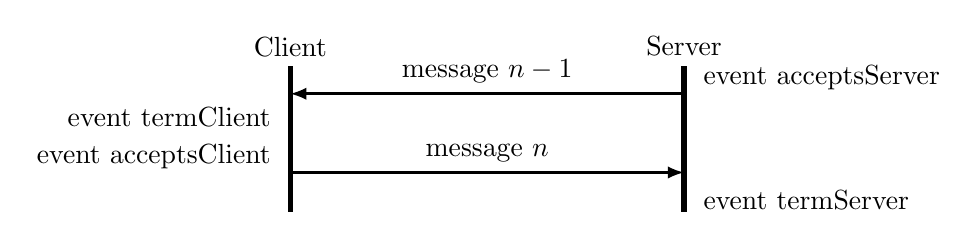
\begin{tikzpicture}[
		derivation/.style = {draw,regular polygon, regular polygon sides=3, minimum size=2.3cm },
		rule/.style = {draw, rounded corners},
		auto
			]
		\node (Client) at (0,2.1) {Client};
		\node (Server) at (5,2.1) {Server};

		\node [label=right:event acceptsServer] at (5,1.7) {};
		\node [label=right:event termServer] at (5,0.15){};

		\node [label=left:event termClient] at (0,1.2) {};
		\node [label=left:event acceptsClient] at (0,0.7) {};

		\path[latex-,line width=1pt]  (0,1.5) edge node {message $n-1$} (5,1.5);
		\path [-latex,line width=1pt] (0,0.5) edge node {message $n$} (5,0.5);

		\draw [line width=2pt] (0,0) -- (Client);
		\draw [line width=2pt] (5,0) -- (Server);

	\end{tikzpicture}
%    \begin{pspicture}(0,0)(5,2.5)
%      %\psgrid
%      \put(-0.5,2.1){Client}
%      \psline[linewidth=2pt](0,0)(0,2)
%      \put(4.4,2.1){Server}
%      \psline[linewidth=2pt](5,0)(5,2)
%      \put(5.1,1.6){event acceptsServer}
%      \put(1.4,1.7){message $n-1$}
%      \psline[arrows=<-,arrowsize=5pt](0,1.5)(5,1.5)
%      \put(-2.6,1.1){event termClient}
%      \put(-3,0.6){event acceptsClient}
%      \put(1.7,0.7){message $n$}
%      \psline[arrows=->,arrowsize=5pt](0,0.5)(5,0.5)
%      \put(5.1,0.1){event termServer}
%    \end{pspicture}
\end{center}
\caption{Messages and events for authentication}
\label{fig:mess_events}
\end{figure}
%
There is generally some flexibility in the placement of events in a process,
%There is room for choice for placing the events in the code of the protocol,
but not all choices are correct.
For example, in order to prove authentication %one proves properties of the form
in our handshake protocol, we consider the property
\begin{lstlisting}[numbers=none]
query x:key; inj-event(termServer(x))==>inj-event(acceptsClient(x)).
\end{lstlisting}
and the event \lstinline!termServer! is placed when the server terminates (typically at the end of the protocol), while \lstinline!acceptsClient! is placed when the client accepts (typically before the client sends its last message). Therefore, when the last message, message $n$, is from the client to the server, the placement of events follows Figure~\ref{fig:mess_events}: the last message sent by the client is message $n$, so \lstinline!acceptsClient! is placed before the client sends message $n$, and \lstinline!termServer! is placed after the server receives message $n$. The last message sent by the server is message $n-1$, so  \lstinline!acceptsServer! is placed before the server sends message $n-1$, and \lstinline!termClient! is placed after the client receives message $n-1$ (any position after that reception is fine).
%
More generally, the event that occurs before the arrow \lstinline!==>!
can be placed at the end of the protocol, but the event that occurs
after the arrow \lstinline!==>! must be followed by at least one
message output. Otherwise, the whole protocol can be executed without
executing the latter event, so the correspondence certainly does not
hold.

One can also note that moving an event that occurs before the arrow
\lstinline!==>! towards the beginning of the protocol strengthens the
correspondence property, and moving an event that occurs after the
arrow \lstinline!==>! towards the end of the protocol also strengthens
the correspondence property. Adding arguments to the events strengthens
the correspondence property as well.

\section{Understanding ProVerif output}\label{sec:output}

The output produced by ProVerif is rather verbatim and can be overwhelming for new users. In essence the output is in the following format:
%
\begin{lstlisting}[numbers=none]
[Equations]
Process:
 [Process]

-- Query [Query]
Completing...
Starting query [Query]
goal [un]reachable: [Goal]
Abbreviations:
 ...

[Attack derivation]

A more detailed output of the traces is available with
  set traceDisplay = long.

[Attack trace]

RESULT [Query] [result].

--------------------------------------------------------------
Verification summary:

[Summary of verification results]

--------------------------------------------------------------
\end{lstlisting}
%
where \lstinline{[Equations]} summarizes the internal representation of the equations given in the input file (if any) and \lstinline{[Process]} presents the input process with all macros expanded and distinct identifiers assigned to unique names/variables; in addition, parts of the process are annotated with identifiers {\tt \{$n$\}} where $n\in\mathbb{N}^*$. (New users may like to refer to this interpreted process to ensure they have defined the scope of variables in the correct manner and to ensure they haven't inadvertently bound processes inside if-then-else/let-in-else statements.) ProVerif then begins to evaluate the \lstinline{[Query]} provided by the user. Internally, ProVerif attempts to prove that a state in which a property is violated is unreachable; it follows that ProVerif shows the (un)reachability of some \lstinline{[Goal]}. If a property is violated then ProVerif attempts to reconstruct an \lstinline{[Attack derivation]} in English and an \lstinline{[Attack trace]} in the applied pi calculus. ProVerif then reports whether the query was satisfied. Finally, ProVerif displays a summary of the verification results of all the queries in the file. For convenience, Linux and cygwin users may make use of the following command:
\[
	\texttt{./proverif $\filenamevar$.pv | grep "RES"}
\]
which reduces the output to the results of the queries. %A more detailed discussion of ProVerif output is presented in Section~\ref{sec:proverifOutput}.

\subsection{Results}

In order to understand the results correctly, it is important to understand the difference between the attack derivation and the attack trace. The attack derivation is an explanation of the actions that the attacker has to make in order to break the security property, in the internal representation of ProVerif. Because this internal representation uses abstractions, the derivation is not always executable in reality; for instance, it may require the repetition of certain actions that can in fact never be repeated, for instance because they are not under a replication. In contrast, the attack trace refers to the semantics of the applied pi calculus, and always corresponds to an executable trace of the considered process.

ProVerif can display three kinds of results:
\begin{itemize}

\item \lstinline!RESULT [Query] is true!: The query is proved, there
  is no attack. In this case, ProVerif displays no attack
  derivation and no attack trace.

\item \lstinline!RESULT [Query] is false!: The query is false,
  ProVerif has discovered an attack against the desired security
  property. The attack trace is displayed just before the result
  (and an attack derivation is also displayed, but you should focus on
  the attack trace since it represents the real attack).

\item \lstinline!RESULT [Query] cannot be proved!: This is a ``don't
  know'' answer. ProVerif could not prove that the query is true and
  also could not find an attack that proves that the query is false.
  Since the problem of verifying protocols for an unbounded number of
  sessions is undecidable, this situation is unavoidable.
  Still, ProVerif gives some additional information that can be useful
  in order to determine whether the query is true. In particular,
  ProVerif displays an attack derivation. By manually inspecting the
  derivation, it is sometimes possible to reconstruct an attack.  For
  observational equivalence properties, it may also display an attack
  trace, even if this trace does not prove that the observational
  equivalence does not hold. We will come back to this point when we
  deal with observational equivalence, in Section~\ref{sec:obsequi}.
  Sources of incompleteness, which explain why ProVerif sometimes
  fails to prove properties that hold, will be discussed in
  Section~\ref{sec:incomplete}.

\end{itemize}

\paragraph{Interpreting results.} Understanding the internal manner in which ProVerif operates is useful to interpret the results output. Recall that ProVerif attempts to prove that a state in which a property is violated is unreachable. It follows that when ProVerif is supplied with \lstinline!query attacker($M$).!, that internally ProVerif attempts to show \lstinline!not attacker($M$)! and hence \lstinline!RESULT not attacker($M$) is true.! means that the secrecy of $M$ is preserved by the protocol.

\paragraph{Error and warning messages.}

In case of a syntax error, ProVerif indicates the character position of the error (line and column numbers). Please use your text editor to find the position of the error. (The error messages can be interpreted by \texttt{emacs}.) In addition, ProVerif may provide various warning messages. The earlier grep command can be modified into \texttt{./proverif $\filenamevar$.pv | egrep "RES|Err|War"} for more manageable output with notification of error/warnings, although a more complex command is required to read any associated messages. In this case, the command \texttt{./proverif $\filenamevar$.pv | less} can be useful.

\subsection{Example: ProVerif output for the handshake protocol}\label{sec:output_handshake}

Executing the handshake protocol with \texttt{./proverif {\docexdir}ex\_handshake\_annotated.pv | grep "RES"} produces the following output:
%
\begin{lstlisting}[numbers=none]
RESULT not attacker(s[]) is false.
RESULT event(termClient(x_2,y_1)) ==> event(acceptsServer(x_2,y_1)) is false.
RESULT inj-event(termServer(x_2)) ==> inj-event(acceptsClient(x_2)) is true.
\end{lstlisting}
%
which informs us that authentication of $\A$ to $\B$ holds, but authentication of $\B$ to $\A$ and secrecy of $s$ do not hold.


\subsubsection{Analyzing attack traces.}

By inspecting the output more closely, we can reconstruct the attack. For example, let us consider the query
\lstinline!query attacker(s)! which produces the following:
%
\begin{lstlisting}
Process 0 (that is, the initial process):
{1}new skA: skey;
{2}new skB: sskey;
{3}let pkA: pkey = pk(skA) in
{4}out(c, pkA);
{5}let pkB: spkey = spk(skB) in
{6}out(c, pkB);
(
    {7}!
    {8}out(c, pkA);
    {9}in(c, x: bitstring);
    {10}let y: bitstring = adec(x,skA) in
    {11}let (=pkB,k: key) = checksign(y,pkB) in
    {12}event acceptsClient(k);
    {13}out(c, senc(s,k));
    {14}event termClient(k,pkA)
) | (
    {15}!
    {16}in(c, pkX: pkey);
    {17}new k_1: key;
    {18}event acceptsServer(k_1,pkX);
    {19}out(c, aenc(sign((pkB,k_1),skB),pkX));
    {20}in(c, x_1: bitstring);
    {21}let z: bitstring = sdec(x_1,k_1) in
    {22}if (pkX = pkA) then
    {23}event termServer(k_1)
)

-- Query not attacker(s[]) in process 0.
Completing...
Starting query not attacker(s[])
goal reachable: attacker(s[])

Derivation:
Abbreviations:
k_2 = k_1[pkX = pk(sk),!1 = @sid]

1. The attacker has some term sk.
attacker(sk).

2. By 1, the attacker may know sk.
Using the function pk the attacker may obtain pk(sk).
attacker(pk(sk)).

3. The message pk(sk) that the attacker may have by 2 may be received at
input {16}.
So the message aenc(sign((spk(skB[]),k_2),skB[]),pk(sk)) may be sent to the
attacker at output {19}.
attacker(aenc(sign((spk(skB[]),k_2),skB[]),pk(sk))).

4. By 3, the attacker may know aenc(sign((spk(skB[]),k_2),skB[]),pk(sk)).
By 1, the attacker may know sk.
Using the function adec the attacker may obtain sign((spk(skB[]),k_2),skB[]).
attacker(sign((spk(skB[]),k_2),skB[])).

5. By 4, the attacker may know sign((spk(skB[]),k_2),skB[]).
Using the function getmess the attacker may obtain (spk(skB[]),k_2).
attacker((spk(skB[]),k_2)).

6. By 5, the attacker may know (spk(skB[]),k_2).
Using the function 2-proj-2-tuple the attacker may obtain k_2.
attacker(k_2).

7. The message pk(skA[]) may be sent to the attacker at output {4}.
attacker(pk(skA[])).

8. By 4, the attacker may know sign((spk(skB[]),k_2),skB[]).
By 7, the attacker may know pk(skA[]).
Using the function aenc the attacker may obtain
aenc(sign((spk(skB[]),k_2),skB[]),pk(skA[])).
attacker(aenc(sign((spk(skB[]),k_2),skB[]),pk(skA[]))).

9. The message aenc(sign((spk(skB[]),k_2),skB[]),pk(skA[])) that the attacker
may have by 8 may be received at input {9}.
So the message senc(s[],k_2) may be sent to the attacker at output {13}.
attacker(senc(s[],k_2)).

10. By 9, the attacker may know senc(s[],k_2).
By 6, the attacker may know k_2.
Using the function sdec the attacker may obtain s[].
attacker(s[]).

11. By 10, attacker(s[]).
The goal is reached, represented in the following fact:
attacker(s[]).


A more detailed output of the traces is available with
  set traceDisplay = long.

new skA: skey creating skA_1 at {1}

new skB: sskey creating skB_1 at {2}

out(c, ~M) with ~M = pk(skA_1) at {4}

out(c, ~M_1) with ~M_1 = spk(skB_1) at {6}

out(c, ~M_2) with ~M_2 = pk(skA_1) at {8} in copy a

in(c, pk(a_1)) at {16} in copy a_2

new k_1: key creating k_2 at {17} in copy a_2

event acceptsServer(k_2,pk(a_1)) at {18} in copy a_2

out(c, ~M_3) with ~M_3 = aenc(sign((spk(skB_1),k_2),skB_1),pk(a_1)) at {19}
in copy a_2

in(c, aenc(adec(~M_3,a_1),~M)) with aenc(adec(~M_3,a_1),~M) =
aenc(sign((spk(skB_1),k_2),skB_1),pk(skA_1)) at {9} in copy a

event acceptsClient(k_2) at {12} in copy a

out(c, ~M_4) with ~M_4 = senc(s,k_2) at {13} in copy a

event termClient(k_2,pk(skA_1)) at {14} in copy a

The attacker has the message
sdec(~M_4,2-proj-2-tuple(getmess(adec(~M_3,a_1)))) = s.
A trace has been found.
RESULT not attacker(s[]) is false.

\end{lstlisting}

ProVerif first outputs its internal representation of the process under consideration.
Then, it handles each query in turn. The output regarding the query \lstinline!query attacker(s)!
can be split into three main parts:
\begin{itemize}
\item From ``\lstinline!Abbreviations!'' to ``\lstinline!A more detailed...!'', a description of the derivation
that leads to the fact \lstinline!attacker(s)!.
\item After ``\lstinline!A more detailed...!'' until ``\lstinline!A trace has been found!'', a description
of the corresponding attack trace.
\item Finally, the ``\lstinline!RESULT!'' line concludes: the property is false, there is an attack
in which the attacker gets \lstinline!s!.
\end{itemize}
Let us first explain the derivation. It starts with a list of abbreviations: these abbreviations give names to some subterms, in order to display them more briefly; such abbreviations are used for the internal representation of names (keys, nonces, \ldots), which can sometimes be large terms that represent simple atomic data. Next, the description of the derivation itself starts. It is a numbered list of steps, here from 1 to 10. Each step corresponds to one action of the process or of the attacker. After an English description of the step, ProVerif displays the fact that is derived thanks to this step, here \lstinline!attacker($M$)! for some term $M$, meaning that the attacker has $M$.
\begin{itemize}
\item In step 1, the attacker chooses any value \lstinline!sk! in its knowledge (which it is going to use as its secret key).
\item In step 2, the attacker uses the knowledge of \lstinline!sk! obtained at step 1 (``\lstinline!By 1!'') to compute the corresponding public key \lstinline!pk(sk)! using function \lstinline!pk!.
\item Step 3 is a step of the process. Input \lstinline!{16}! (the numbers between braces refer to program points also written between braces in the description of the process, so input \lstinline!{16}! is the input of Line~19) receives the message \lstinline!pk(sk)! from the attacker, and output \lstinline!{19}! (the one at Line~22) replies with \lstinline!aenc(sign((spk(skB[]),k_2),skB[]),pk(sk))!. Note that \lstinline!k_2! is an abbreviation for \lstinline{k_2 = k_1[pkX = pk(sk),!1 = @sid]}, as listed at the beginning of the derivation. It designates the key \lstinline!k_2! generated by the \lstinline!new! at Line~20, in session \lstinline!@sid! (the number of the copy generated by the replication at Line~18, designated by \lstinline{!1}, that is, the first replication), when the key \lstinline!pkX! received by the input at Line~19 is \lstinline!pk(sk)!. ProVerif displays \lstinline!skB[]! instead of \lstinline!skB! when \lstinline!skB! is a name without argument (that is, a free name or a name chosen under no replication and no input). In other words, the attacker starts a session of the server $B$ with its own public key and gets the corresponding message \lstinline!aenc(sign((spk(skB[]),k_2),skB[]),pk(sk))!.
\item Steps 4 to 6 are again applications of functions by the attacker to perform its internal computations: the attacker decrypts the message
\lstinline!aenc(sign((spk(skB[]),k_2),skB[]),pk(sk))! received at step 3 and gets the signed message, so it obtains
\lstinline!sign((spk(skB[]),k_2),skB[])! (step 4) and \lstinline!k_2! (step 6).
\item Step 7 uses a step of the process: by the output \lstinline!{4}! (the one at Line~5), the attacker gets \lstinline!pk(skA[])!.
\item At step 8, the attacker reencrypts \lstinline!sign((spk(skB[]),k_2),skB[])! with \lstinline!pk(skA[])!.
\item Step 9 is again a step of the process: the attacker sends \lstinline!aenc(sign((spk(skB[]),k_2),skB[]),pk(skA[]))! (obtained at step 8) to input \lstinline!{9}! (at Line~11) and gets the reply \lstinline!senc(s[],k_2)!. In other words, the attacker has obtained a correct message 2 for a session between $A$ and $B$. It sends this message to $A$ who replies with \lstinline!senc(s[],k_2)! as if it was running a session with $B$.
\item In step 10, the attacker decrypts \lstinline!senc(s[],k_2)! since it has \lstinline!k_2! (by step 6), so it obtains \lstinline!s[]!.
\item Finally, step 11 indicates that the query goal has been reached, that is, \lstinline!attacker(s[])!.
\end{itemize}

As one can notice, this derivation corresponds exactly to the attack against the protocol outlined in Figure~\ref{fig:handshakeprotocol}. The display of the derivation can be tuned by some settings: \lstinline!set abbreviateDerivation = false! prevents the use of abbreviations for names and \lstinline!set explainDerivation = false! switches to a display of the derivation by explicit references to the Horn clauses used internally by ProVerif instead of relating the derivation to the process. (See also Section~\ref{sec:settings} for details on these settings.)

Next, ProVerif reconstructs a trace in the semantics of the pi calculus, corresponding to this derivation. This trace is presented as a sequence of inputs and outputs on public channels and of events. The internal reductions of the process are not displayed for brevity. (As mentioned in the output, it is possible to obtain a more detailed display with the state of the process and the knowledge of the attacker at each step by adding \lstinline!set traceDisplay = long.! in your input file.) Each input, output, or event is followed by its location in the process ``\lstinline!at {$n$}!'', which refers to the program point between braces in the process displayed at the beginning. When the process is under replication, several copies of the process may be generated. Each of these copies is named (by a name like ``\lstinline!a_$n$!''), and ProVerif indicates in which copy of the process the input, output, or event is executed. The name itself is unimportant, just the fact that the copy is the same or different is important: the presence of different names of copies for the same replication shows that several sessions are used. Let us explain the trace in the case of the handshake protocol:



\begin{itemize}
\item The first two \lstinline!new! correspond to the creation of secret keys.

\item The first two outputs correspond to the outputs of public keys, at outputs \lstinline!{4}! (Line~5) and \lstinline!{6}! (Line~7). The attacker stores these public keys in fresh variables \lstinline!~M! and \lstinline!~M_1! respectively, so that it can reuse them later.

\item The third output is the output of \lstinline!pkA! at output \lstinline!{8}! (Line~10), in a session of the client $A$ named \lstinline!a!.

\item The next 4 steps correspond to a session of the server $B$ (copy \lstinline!a_2!) with the attacker: the attacker sends its public key \lstinline!pk(a_1)! at the input \lstinline!{16}! (Line~19). A fresh shared key \lstinline!k_2! is then created. The event \lstinline!acceptsServer! is executed (Line~21), and the message \lstinline!aenc(sign((spk(skB_1),! \lstinline!k_2),! \lstinline!skB_1),! \lstinline!pk(a_1))! is sent at output \lstinline!{19}! (Line~22) and stored in variable \lstinline!~M_3!, a fresh variable that can be used later by the attacker. These steps correspond to step 3 of the derivation above.

\sloppy

\item The last 4 steps correspond to the end of the execution of the session \lstinline!a! of the client $A$. The attacker computes \lstinline!aenc(adec(~M_3,a_1),~M))! and obtains the message \lstinline!aenc(sign((spk(skB_1),k_2),skB_1),pk(skA_1))!, which it sends to the input \lstinline!{9}! (Line~11). The event \lstinline!acceptsClient! is executed (Line~14), the message \lstinline!senc(s,k_2)! is sent at output \lstinline!{13}! (Line~15) and stored in variable \lstinline!~M_4! and finally the event \lstinline!termClient! is executed (Line~16). These steps correspond to step 9 of the derivation above.

\fussy

\item Finally, the attacker obtains \lstinline!s[]! by computing \lstinline!sdec(~M_4,! \lstinline!2-proj-2-tuple(getmess(adec(!\allowbreak\lstinline!~M_3,! \lstinline!a_1))))!.
\end{itemize}
This trace shows that there is an attack against the secrecy of \lstinline!s!, it corresponds to the attack against the protocol outlined in Figure~\ref{fig:handshakeprotocol}.

\begin{figure}[ht]
\begin{center}
\includegraphics[width=15cm]{examples/ex_handshakeattackgraph.png}
\end{center}

\caption{Handshake protocol attack trace}
\label{fig:handshakeprotocolgraphtrace}
\end{figure}

Another way to represent an attack found by ProVerif is by a graph. For instance, the attack explained previously is shown in Figure~\ref{fig:handshakeprotocolgraphtrace}. To obtain such a graph, use the command-line option \texttt{-graph} or \texttt{-html} described in Section~\ref{sec:command-line}. The detailed version is built when
  \lstinline!set traceDisplay = long.! has been added to the input \texttt{.pv} file.
The graph starts always with two processes: the honest one, and the attacker. The progress of the attack is represented vertically. Parallel processes are represented by several columns. Replications of processes are denoted by nodes labeled by \lstinline$!$, with a column for each created process. Processes fork when a parallel composition is reduced. The termination of a process is represented by a point. An output on a public channel is represented by a horizontal arrow from the process that makes the output to the attacker. The edge is labeled with an equality $X = M$ where $M$ is the sent message and $X$ is a fresh variable (or tuple of variables) in which the adversary stores it. An input on a public channel is represented by an arrow from the attacker to the receiving process, labeled with an equality $R = M$, where $R$ is the computation performed by the attacker to obtain the sent message $M$. The message $M$ is omitted when it is exactly equal to $R$, for instance when $R$ is a constant. A communication made on a private channel is represented by an arrow from the process that outputs the message to the process that receives it; this arrow is labeled with the message. Creation of nonces and other steps are represented in boxes. Information about the attack is written in red; the displayed information depends on the security property that is broken by the attack. The text ``a trace has been found'' is written at the top of the figure, possibly with assumptions necessary for the attack.  When labels are too long to fit on arrows, a table of abbreviations  appears at the top right of the figure.

Let us take a closer look at Figure~\ref{fig:handshakeprotocolgraphtrace}. First, two new secret keys are created by the honest process. Then the corresponding public keys are sent on a public channel; the attacker receives them and stores them in \lstinline!~M! and \lstinline!~M_1!. Next, a parallel reduction is made. We obtain two processes which replicate themselves once each. The first process (\lstinline!clientA!) sends its public key on a public channel, and the attacker receives it. Then the attacker sends the message \lstinline!pk(a_1)!, containing its own public key, to the second process \lstinline!serverB!. This process then creates a new shared key \lstinline!k_2! and executes the event  \lstinline!acceptsServer(k_2,pk(a_1))!. It sends the message \lstinline!aenc(sign((spk(skB_1),! \lstinline!k_2),! \lstinline!skB_1),! \lstinline!pk(a_1))! on a public channel; the attacker receives it and stores it in \lstinline!~M_3!. The attacker computes \lstinline!aenc(adec(~M_3,a_1),~M))!, that is, it decrypts and reencrypts the message, thus obtaining \lstinline!aenc(sign((spk(skB_1),k_2),skB_1),pk(skA_1))!. It sends that message to \lstinline!clientA!. The process \lstinline!clientA! executes the event \lstinline!acceptsClients(k_2)! and sends the message \lstinline!senc(s,k_2)!. The attacker receives it and stores it in \lstinline!~M_4!. Finally, the attacker computes \lstinline!sdec(~M_4,2-proj-2-tuple(getmess(adec(~M_3,a_1))))!, and obtains the secret \lstinline!s!. This point is mentioned in the red box at the bottom right of the page. The process \lstinline!clientA! executes the last event \lstinline!termClient!, and terminates. This is the end of the attack. The line numbers of each step appear in green in boxes. The keywords are written in blue, while the names of processes are written in green.





%\subsubsection{Fixing the handshake protocol.}
For completeness, we present the complete formalization of the rectified protocol, which ProVerif can successfully verify, below and in the file \texttt{{\docexdir}ex\_handshake\_annotated\_fixed.pv}.

\lstinputlisting{examples/ex_handshake_annotated_fixed.pv}

% in Figures~\ref{fig:handshakeFixed} \&~\ref{fig:handshakeFixed2}; which ProVerif can successfully verify.

%\begin{figure}[tbhp!]
%\lstinputlisting[firstnumber=1,linerange={1-28}]{examples/ex_handshake_annotated_fixed.pv}
%\caption{Fixed handshake protocol modeled in ProVerif: Top matter}
%\label{fig:handshakeFixed}
%\end{figure}

%\begin{figure}[tbhp!]
%\lstinputlisting[firstnumber=29,linerange={32}]{examples/ex_handshake_annotated_fixed.pv}
%\caption{Fixed handshake protocol modeled in ProVerif: Main process and security properties}
%\label{fig:handshakeFixed2}
%s\end{figure}
%
% \begin{figure}[ht]
% \begin{center}
% \includegraphics[width=15cm]{handshakeattackgraph.eps}
% \end{center}

% \caption{Handshake Protocol Attack Trace}
% \label{fig:handshakeprotocolgraphtrace}
% \end{figure}


% Another way to represent an attack found by Proverif is by a graph: for instance, Figure~\ref{fig:handshakeprotocolgraphtrace} represents the attack explained previously. To obtain such a graph, use the command \texttt{-graph} or \texttt{-html} described in Section~\ref{sec:command-line}. The detailed version of the attack is built when
%   \lstinline!set traceDisplay = long.! has been added to the input \texttt{.pv} file.


\section{Interactive mode}\label{secroverif_interact}
As indicated in Section~\ref{sec:install}, ProVerif comes with a program \texttt{proverif\_interact} which allows to simulate the execution of a process run. There are two ways to launch this program. By typing the name of the program. It then opens a file chooser dialog allowing to choose a \texttt{.pv} or \texttt{.pcv} file containing the description of the protocol. (\texttt{.pcv} files are for CryptoVerif compatibility, see Section~\ref{sec:cryptoverif}. To choose a \texttt{.pcv} file, you first need to change the filter at the bottom right of the file chooser dialog.) The other way is by typing the name of the program, followed by the path of the \texttt{.pv} or \texttt{.pcv} file. In this case, the simulator starts directly.
When the input file is correctly loaded, a window appears, as in Figure~\ref{fig:simulator_window_0}, where the loaded file is the model of the handshake protocol, available in \texttt{{\docexdir}ex\_handshake.pv}.



% \begin{center}\label{simulator_window_0}
% \includegraphics[width=10cm]{examples/simulator_window_0.eps}
% \end{center}

\subsection{Interface description}\label{sec:interact_interface_desc}
The simulator is made of a main window which allows to make reduction steps on running processes. This window contains several columns representing the current state of the run. The first column, titled ``Public'', contains all public elements of the current state. For example, after loading the file containing the handshake protocol, the channel $c$ appears in the public column as expected, since $c$ is declared public in the input file (see Figure~\ref{fig:simulator_window_0}).  The last columns show processes that are currently running in parallel. To make a reduction step on a specific process, you can click on the head of the column representing the process to reduce. To allow the attacker to create a nonce, there is a button ``New nonce'', or an option in the ``Reduction'' menu, or a keyboard shortcut Ctrl$+$C. If the types are not ignored (by including \lstinline!set ignoreTypes = false! in your input file, see Section~\ref{sec:settings}), a dialog box opens and asks the type of the nonce. When a nonce is created, it is added to the public elements of the current state. To go one step backward, there is a button ``Backward'', or an option in the ``Reduction'' menu, or a keyboard shortcut Ctrl$+$B. The button ``Forward'', the option ``Forward'' of the ``Reduction'' menu, or the keyboard shortcut Ctrl$+$F allow the user to re-execute a step that has been undone by the ``Backward'' button. The button ``Add a term to public '' is explained in Section~\ref{sec:create_public_term}. The interface also allows to display a drawing of the current trace in a new window by clicking on ``Display trace'' in the ``Show'' menu, or by hitting  Ctrl$+$D. Each time a new reduction step is made, the drawing is refreshed. The trace can be saved by selecting ``Save File'' in the  ``Save'' menu, or hitting Ctrl$+$S. One of these formats: \texttt{.png, .pdf, .jpg or .eps}, must be used to save the file, and the name of the file with its extension must be given. Note that a more detailed version of the trace is available if \lstinline!set traceDisplay = long.! has been added to the input file. The main window and the menu also contains two other options: ``Next auto-step'' and ``All auto-steps''. We explain this functionality in the next section.

\begin{figure}
\begin{center}
\includegraphics[width=10cm]{simulator_window_0.png}
  \caption{Handshake protocol - Initial simulator window}
  \label{fig:simulator_window_0}
\end{center}
\end{figure}

\subsection{Manual and auto-reduction}\label{sec:manual_and_auto_reduction}
There are two kinds of processes. The ones on which the first reduction can be done without the intervention of the user (called auto-reducible processes), and the ones that require the intervention of the user (called manually-reducible processes).
\begin{itemize}

\sloppy

\item The processes \lstinline!0!, \lstinline!$P$ | $Q$!, \lstinline!new $n:t$; $P$!, \lstinline!let $x = M$ in $P$ else $Q$!, \lstinline!if $M$ then $P$ else $Q$!, and \lstinline!event $e(M_1,\dots,M_n)$; $P$! are all auto-reducible.

\fussy

\item The process \lstinline:!P: is manually reducible.
\item The process \lstinline!out$(M,N)$; $P$! is auto-reducible if the channel $M$ is public, or the evaluation of the message $N$ or of the channel $M$ fails. Otherwise, it is a manually-reducible process.
\item The process \lstinline!in$(M,x:T)$; $P$! is auto-reducible if the evaluation of the channel $M$ fails. Otherwise, it is a manually-reducible process.
%% \item The process  \lstinline!insert $d(M_1,\ldots,M_n)$!, is auto-reducible if it is the only process, or if the evaluation of one of the $M_i$ fails (see Section~\ref{sec:tables} for more information on \lstinline!insert!).
%% \item All other processes are manually-reducible processes and require the intervention of the user: get, phase.
%% \item Note that the processes \lstinline!let...suchthat...! (see Section~\ref{sec:predicates}) and  \lstinline!sync! (see Section~\ref{sec:sync}) are not supported yet.
\end{itemize}
When auto-reducible processes are running and you press the button ``All auto-steps'' (or if you select this option on the menu), it reduces all auto-reducible processes that are running. When you press the button ``Next auto-step'', it makes one step of reduction on the first auto-reducible process.
Manually-reducible processes can be reduced only by clicking on the head of their column.

\subsection{Execution of $0$, $P$  \lstinline!|!  $Q$, $!P$, new, let, if, and event}
The reduction of \lstinline!0! just removes the process. The reduction of \lstinline!$P$ | $Q$! separates the process \lstinline!$P$ | $Q$! into two processes $P$ and $Q$ (a column is added to the main window). The reduction of \lstinline:$!P$: adds a copy of $P$ in a new column at the left of  \lstinline:$!P$:. The reduction of \lstinline!new $n:t; P$! creates a fresh nonce local to the process $P$. The reduction of \lstinline!let $x = M$ in $P$ else $Q$! evaluates $M$. If this evaluation succeeds, then the process becomes $P$ with the result of $M$ substituted for $x$. Otherwise, the process becomes $Q$. The reduction of \lstinline!if $M$ then $P$ else $Q$! evaluates $M$. If $M$ evaluates to \lstinline!true!, then the process becomes $P$. If the evaluation of $M$ succeeds and $M$ evaluates to a value other than \lstinline!true!, then the process becomes $Q$. If the evaluation of $M$ fails, then the process is removed. The reduction of \lstinline!event $e(M_1,\dots,M_n)$; $P$! evaluates $M_1, \dots, M_n$. If these evaluations succeed, the process becomes $P$. Otherwise, the process is removed. The user can display a column titled ``Events'', showing the list of executed events by selecting the item ``Show/hide events'' in the ``Show'' menu or using the keyboard shortcut Ctrl$+$E.


\subsection{Execution of inputs and outputs}\label{sec:input_output_simulation}
They are several possible kinds of inputs and outputs, depending on whether the process is auto-reducible or not, and on whether the channel is public or not.
Let us first consider the case of \lstinline!out$(M,N)$; $P$!.
\begin{itemize}
\item If the process is auto-reducible because the evaluation of the channel $M$ or of the message $N$ fails, then the process is removed.

\item If the evaluations of the message $N$ and the channel $M$ succeed and the channel $M$ is public, then the output is made as explained in Section~\ref{sec:main}. The message is added to the public elements of the current state. It is displayed as follows \lstinline!~M_$i$ = $N$!, where \lstinline!~M_$i$! is a new binder: this binder can then be used to designate the term $N$ in the computations that the adversary makes in the rest of the execution. Such computations are called \emph{recipes}. They are terms built from the binders \lstinline!~M_$i$!, the nonces created by the adversary, the names that are initially public, and application of public functions to recipes. In the general case, the public elements of the current state are represented in the form $\mathit{binder} = \mathit{recipe} = \mathit{message}$, where the recipe is the computation that the adversary makes to obtain the corresponding message, and the binder can be used to designate that message in future recipes. To lighten the display, the binder is omitted when it is equal to the recipe, and the recipe is omitted when it is equal to the message itself.

\item If the evaluations of the message $N$ and the channel $M$ succeed but the channel $M$ is not known to be public (this case is displayed ``Output (private)'' in the head of the column), then there are two possibilities.
\begin{itemize}
\item Prove that the channel is in fact public, and make a public communication. To do so, a recipe using public elements of the current state must be given. If this recipe is evaluated as equal to the channel, a public output on this channel is made.
\item Make a private communication on this channel between two processes. If this choice has been made, the list of all the input processes on the same channel appears in the main window. The user chooses the process that will receive the output message. If there is no such process, the reduction is not possible and an error message appears.
\end{itemize}
\end{itemize}
Let us now consider the case of \lstinline!in($M$,$x:T$); $P$!.
\begin{itemize}
\item If the evaluation of the channel $M$ fails, then the process is removed.

\item If the evaluation of the channel $M$ succeeds and the channel is public, then a pop-up window opens, and the user gives the message to send on the channel.
The message is given in the form of a recipe, which can contain recipes of public elements of the current state, and applications of public functions.
 In case the recipe is wrongly typed, if types are ignored (the default), then a warning message box appears, allowing the user to choose to continue or go back. If types are not ignored (the input file contains \lstinline!set ignoreTypes = false!), an error message box appears, and a new message must be given.

\item If the evaluation of the channel $M$ succeeds and the channel is not known to be public (this case is displayed ``Input (private)'' in the head of the column), then the program works similarly to the case of a private output. There are again two possibilities: prove that the channel is public by giving a recipe and make an input from the adversary, or choose an output process to make a private communication between these processes as explained above.

\end{itemize}
In addition to the public functions explicitly defined in the input file, recipes can also contain projection functions.
 The syntax for projections associated to tuples differs depending on whether types are ignored or not. If types are ignored (the default), then the $i$-th projection of a tuple of arity $m$ is written \lstinline!$i$-proj-$m$-tuple!. Otherwise, when the input file contains \lstinline!set ignoreTypes = false!, \lstinline!$i$-proj-<$\mathit{type}_1$>-!~$\ldots$~\lstinline!-<$\mathit{type}_m$>-tuple! is the $i$-th projection of a tuple of arity $m$, when \lstinline!<$\mathit{type}_n$>! is the type of the $n$-th argument of the tuple. For instance, \lstinline!2-proj-channel-bitstring-tuple! is the second projection of a pair with arguments of type \lstinline!channel! and \lstinline!bitstring!, so \lstinline!2-proj-channel-bitstring-tuple((c,!\allowbreak\lstinline!m)) = m!, where \lstinline!c! is a channel and \lstinline!m! is a bitstring.
The $i$-th projection of a previously defined data constructor $f$ (see Section~\ref{sec:typeConversion}) is written \lstinline!$i$-proj-$f$!.

\subsection{Button ``Add a term to public''}\label{sec:create_public_term}

Please recall that the elements in public are of the form $\mathit{binder} = \mathit{recipe} = \mathit{message}$ (see Section~\ref{sec:input_output_simulation} for more information on public elements).
Clicking the button ``Add a term to public'' allows the user to add a public term to the current state computed by attacker. The user gives the recipe that the attacker uses to compute this term. It is then evaluated. If the evaluation fails, an error message appears. If the evaluation succeeds, an entry \lstinline!~M_$i = \mathit{recipe} = \mathit{t}$! is added to the column ``Public'', where $t$ is the result of the evaluation of the recipe and \lstinline!~M_$i$! is a fresh binder associated to it. \lstinline!~M_$i$! can then be used in future recipes in order to represent the term $t$.

\subsection{Execution of insert and get}\label{sec:insert_get}

You can ignore this section if you do not use tables, defined in Section~\ref{sec:tables}.
The constructs \lstinline!insert! and \lstinline!get! respectively insert an element in a table
and read a table.

The process  \lstinline!insert $d(M_1,\ldots,M_n)$; $P$! is auto-reducible if it is the only process or if the evaluation of one of the $M_i$ fails.
To insert an element, just click on the head of the column representing the \lstinline!insert! process to reduce. If the evaluation succeeds, the element is inserted and appears in the column ``Tables''. Otherwise, the process is removed.
The user can display a column titled ``Tables'', containing all elements of tables obtained by \lstinline!insert! steps, by selecting the item ``Show/hide tables'' in the ``Show'' menu or using the keyboard shortcut Ctrl$+$T.

The process \lstinline!get $d(T_1,\dots,T_n)$ suchthat $M$ in $P$ else $Q$! is never auto-reducible.
To  \lstinline!get! an element from a table, click on the head of the column to reduce. Three cases are possible, depending on the set of terms in the table $d$ that match the patterns $T_1, \dots T_n$ and satisfy the condition $M$. First, if there is no such term, then the \lstinline!else! branch of the \lstinline!get! is executed. Second, if there is only one such term, then this term is selected, and the \lstinline!in! branch is executed with the variables of $T_1, \dots T_n$ instantiated to match this term, as explained in Section~\ref{sec:tables}. Or third, if there are several such terms, then a window showing all the possible terms is opened. To make the reduction, double-click on the chosen term.

\subsection{Handshake run in interactive mode}
Let us see how to execute a trace similar to the one represented in Figure~\ref{fig:handshakeprotocolgraphtrace} starting from Figure~\ref{fig:simulator_window_0}.
\begin{itemize}
\item First, a click on the ``All auto-steps'' button will lead to the situation represented in Figure~\ref{fig:simulator_window_1}: the honest process first creates two secret keys, then output a first public key after a \lstinline!let!, and then a second one after another \lstinline!let! on channel $c$. The attacker stores these public keys in fresh variables \lstinline!~M_2! and \lstinline!~M_3!. A parallel reduction is then made after that.


\begin{figure}
\begin{center}
\includegraphics[width=15cm]{simulator_window_1.png}
  \caption{Handshake protocol - Simulator window 1}
  \label{fig:simulator_window_1}
\end{center}
\end{figure}

\item The first process \lstinline!ClientA! can now be replicated, by clicking ``Replication'' at the top of its column. Three processes are obtained. The first process can make an output by clicking on ``Next auto-step''.
\item The process \lstinline!ServerB! is then replicated by clicking on the column representing the third process. A click on ``New nonce'' allows the attacker to create his secret key $n$, which is added to the public elements of the current state. The message \lstinline!pk(n)! can then be input on channel \lstinline!c! by clicking on the same column and giving \lstinline!pk(n)! as recipe. The result is shown in Figure~\ref{fig:simulator_window_2}.

\begin{figure}
\begin{center}
\includegraphics[width=15cm]{simulator_window_2.png}
  \caption{Handshake protocol - Simulator window 2}
  \label{fig:simulator_window_2}
\end{center}
\end{figure}

\item A new click on the third process creates a fresh key \lstinline!k_2!. Another click sends the message \lstinline!aenc(sign(spk(skB_2), k_2), skB_2, pk(n))!, and the attacker stores this message in a fresh variable \lstinline!~M_4!.
\item The message \lstinline!aenc(adec(~M_4, n),~M_2)! can then be input on channel \lstinline!c!, by clicking on the first process and giving \lstinline!aenc(adec(~M_4, n),~M_2)! as recipe.
\item A click on the ``All auto-steps'' makes all possible reductions on the first process, leading to the output of the message \lstinline!senc(s, k_2)! stored by the attacker in a variable \lstinline!~M_5!. It leads to the window represented in Figure~\ref{fig:simulator_window_3}, and to a trace similar to the one represented in Figure~\ref{fig:handshakeprotocolgraphtrace}.

\sloppy

\item Finally, by clicking the button ``Add a term to public'' and giving the recipe
\lstinline!sdec(~M_5!, \lstinline!2-proj-2-tuple(getmess(adec(~M_4,n))))!, the attacker computes this recipe and obtains the secret \lstinline!s!. The secret \lstinline!s! is then added to the set of public terms.

\fussy

\begin{figure}
\begin{center}
\includegraphics[width=15cm]{simulator_window_3.png}
  \caption{Handshake protocol - Simulator window 3}
  \label{fig:simulator_window_3}
\end{center}
\end{figure}
\end{itemize}
%\subsection{Further examples}

\subsection{Advanced features}

If the process representing by the input file contains subterms of the form \lstinline!choice[$L$,$R$]! or \lstinline!diff[$L$,$R$]! (see Section~\ref{sec:obsequi}), a pop-up window will ask the user to choose either the first or the second component of \lstinline!choice!, or the biprocess (process with \lstinline!choice[$L$,$R$]!). If the user choses the first or second component, all instances of \lstinline!choice! inside the process will then be replaced accordingly. Otherwise, the tool runs the processes using the semantics of biprocesses. If the input file is made to test the equivalence between two processes $P_1$ and $P_2$ (see Section~\ref{sec:obsequi}), a pop-up window will ask the user to choose to emulate either $P_1$ or $P_2$.

The processes \lstinline!let ... suchthat ...! (see Section~\ref{sec:predicates}) and  \lstinline!sync! (see Section~\ref{sec:sync}) are not supported yet. Passive adversaries (the setting \lstinline{set attacker = passive.}, see Section~\ref{sec:settings}) and key compromise (the setting \lstinline{set keyCompromise = approx.} or \lstinline{set keyCompromise = strict.}, see Section~\ref{sec:settings}) are not supported either. The simulator always simulates an active adversary without key compromise, even if different settings are present.

The command line options \texttt{-lib [filename]} (see Section~\ref{sec:command-line}), and \texttt{-commandGraph} (used to define the command for the creation of the graph trace from the dot file generated by the simulator) can be used.


%%%%%%%%%%%%%%%%%%%%%%%%%%%%%%%%%%%%%%%%%%%%%%%%%%%%%%%%%%%%%%%%%%%%%%%
%%%%%%%%%%%%%%%%%%%%%%%%%%%%%%%%%%%%%%%%%%%%%%%%%%%%%%%%%%%%%%%%%%%%%%%
%%%%%%%%%%%%%%%%%%%%%%%%%%%%%%%%%%%%%%%%%%%%%%%%%%%%%%%%%%%%%%%%%%%%%%%

\chapter{Language features}\label{sec:advLang}

In the previous chapter, the basic features of the language were introduced; we will now provide a more complete coverage of the language features. These features will be used in Chapter~\ref{sec:caseStudy} to study the Needham-Schroeder public key protocol as a case study. More advanced features of the language will be discussed in Chapter~\ref{sec:advTheory} and the complete input grammar is presented in Appendix~\ref{app:grammar} for reference; the features presented in this chapter should be sufficient for most users.

\section{Primitives and modeling features}

In Section~\ref{sec:topMatter}, we introduced the basic components of the declarations of the language and how to model processes; this section will develop our earlier presentation.

\subsection{Constants}\label{sec:constants}

A constant may be defined as a function of arity $0$, for example ``\lstinline!fun $c(): t$.!'' ProVerif also provides a specific construct for constants:
\begin{lstlisting}[numbers=none]
	const $c: t$.
\end{lstlisting}
where $c$ is the name of the constant and $t$ is its type.
Several constants of the same type $t$ can be declared by
\begin{lstlisting}[numbers=none]
	const $c_1, \dots, c_k: t$.
\end{lstlisting}

\subsection{Data constructors and type conversion}\label{sec:typeConversion}

Constructors \lstinline!fun $f(t_1,\dots,t_n): t$.! may be declared as items of data by appending \lstinline![data]!, that is,
\begin{lstlisting}[numbers=none]
	fun $f(t_1,\dots,t_n): t$ [data].
\end{lstlisting}
A constructor declared as data is similar to a tuple: the attacker can construct and decompose data constructors. In other words, declaring a data constructor $f$ as above implicitly declares $n$ destructors that map $f(x_1, \ldots, x_n)$ to $x_i$, where $i\in\{1,\dots,n\}$. One can inverse a data constructor by pattern-matching: the pattern $f(T_1, \ldots, T_n)$ is added as pattern in the grammar of Figure~\ref{fig:patternGrammar}. The type of $T_1, \ldots, T_n$ is the type of the arguments of $f$, so when $T_i$ is a variable, its type can be omitted. For example, with the declarations
\begin{lstlisting}[numbers=none]
	type key.
	type host.
	fun keyhost(key, host): bitstring [data].
\end{lstlisting}
we can write
\begin{lstlisting}[numbers=none]
	let keyhost(k,h) = x in ...
\end{lstlisting}
Constructors declared \lstinline!data! cannot be declared \lstinline!private!.


One application of data constructors is type conversion. As discussed in Section~\ref{sec:topMatter}, the type system occasionally makes it difficult to apply functions to arguments due to type mismatches. This can be overcome with type conversion. A type converter is simply a special type of data constructor defined as follows:
\begin{lstlisting}[numbers=none]
	fun $tc(t):t'$ [typeConverter].
\end{lstlisting}
where the type converter \lstinline!tc! takes input of type $t$ and returns a result of type $t'$. Observe that, since the constructor is a data constructor, the attacker may recover term $M$ from the term $tc(M)$. Intuitively, the keyword \lstinline!typeConverter! means that the function is the identity function, and so has no effect except changing the type. By default, types are used for typechecking the protocol but during protocol verification, ProVerif ignores types. The \lstinline!typeConverter! functions are thus removed. (This behavior allows ProVerif to detect type flaw attacks, in which the attacker mixes data of different types. This behavior can be changed by the setting \lstinline!set ignoreTypes = ...! as discussed in Section~\ref{sec:settings}.)

The reverse type conversion, from $t'$ to $t$, should be performed by pattern-matching:
\begin{lstlisting}[numbers=none]
	let $tc(x) = M$ in ...
\end{lstlisting}
where $M$ is of type $t'$ and $x$ is of type $t$.
This construct is allowed since type converters are data constructors. When one defines a type converter $tc(t):t'$ from type $t$ to $t'$, all elements of type $t$ can be converted to type $t'$, but the only elements of type $t'$ that can be converted to type $t$ are the elements of the form $tc(M)$. Hence, for instance, it is reasonable to define a type converter from a type \lstinline!key! representing 128-bit keys to type \lstinline!bitstring!, but not in the other direction, since all 128-bit keys are bitstrings but only some bitstrings are 128-bit keys.

\subsection{Natural numbers}\label{sec:naturalNumbers}

Natural numbers are natively supported and have the built-in type \lstinline!nat!. Internally, ProVerif models natural numbers following the Peano axioms, that is, it considers a constant $0$ of type \lstinline!nat! and a data constructor for successor. As such, all natural numbers are terms and can be used with other user-defined functions. A term is said to be \emph{a natural number} if it is the constant $0$ or the application of the successor to a natural number. The grammar of terms (Figure~\ref{fig:grammar}) is extended in Figure~\ref{fig:natural number} to consider the built-in infix functions manipulating natural numbers.

\begin{figure}[ht]
\begin{center}
\begin{minipage}{\linewidth}
\begin{tabbing}
   XX\=XXXXXXXXXXXXXXXXXXXXXXXXXXXXXXXXXxx\=XX\=\kill     %Set tab sizes
$M,N ::=$ \>    				\> terms 		\\
\> ...\>\\
\> $i$					\>\> natural number ($i \in \mathbb{N}$)\\
\> $M + i$							\>\> addition ($i \in \mathbb{N}$)\\
\> $i + M$							\>\> addition ($i \in \mathbb{N}$)\\
\> $M - i$							\>\> subtraction ($i \in \mathbb{N}$)\\
\> $M > N$							\>\> greater \\
\> $M < N$ 							\>\> smaller\\
\> $M >= N$ 							\>\> greater or equal\\
\> $M <= N$ 							\>\> smaller or equal
\end{tabbing}
\end{minipage}
\end{center}
\caption{Natural number grammar}
\label{fig:natural number}
\end{figure}
Finally, ProVerif  has a built-in boolean function \lstinline!is_nat! checking whether a term is a natural number of not, that is, \lstinline!is_nat$(M)$! returns \lstinline!true! if and only if $M$ is equal modulo the equational theory to a natural number.

Note that addition between two arbitrary terms is not allowed. The order relations $>, <, >=, <=$ are internally represented by boolean destructor functions that compare the value of two natural numbers. As such, \lstinline!M > N! returns \lstinline!true! (resp. \lstinline!false!) if $M$ and $N$ are both natural numbers and $M$ is strictly greater than (resp. smaller or equal to) $N$. Note that \lstinline!M > N! fails if $M$ or $N$ is not a natural number.
Similarly, the subtraction is internally represented by a destructor function and for instance, $M - i$ fails if $M$ is a natural number strictly smaller than $i$. It corresponds to the fact that negative numbers are not allowed in ProVerif.

\paragraph{Restrictions.} Since natural numbers are represented with a constant $0$ and a data constructor successor, the attacker can generate all natural numbers. Therefore, ProVerif does not allow the declaration of new names with the type \lstinline!nat!, i.e., \lstinline!new k:nat!, since it would allow a process to generate a term declared as a natural number but that does not satisfy the Peano axioms. Similarly, user defined constructors cannot have \lstinline!nat! as their return type. However, this restriction does not apply to destructors. Finally, all functions can have \lstinline!nat! as argument type. For example, the following declarations and process are allowed.


\begin{lstlisting}
	type key.

	free c:channel.

	free s:bitstring [private].

	fun ienc(nat,key):bitstring.
	fun idec(bitstring,key):nat
	reduc forall x:nat, y:key; idec(ienc(x+1,y),y) = x.

	query attacker(s).

	process
		new k:key; (
		  out(c,ienc(2,k))
		  | in(c,x:nat); in(c,y:bitstring); if x + 3 > idec(y,k) then out(c,s)
		)
\end{lstlisting}

The function \lstinline!idec! is allowed to have \lstinline!nat! as return type as it is declared as a destructor. In this example, the query is false since the attacker can obtain \lstinline!s! by inputting any natural number for \lstinline!x!. Note that the test \lstinline!if x + 3 > idec(y,k) then $\ldots$! is not equivalent to \lstinline!if x > idec(y,k) - 3 then $\ldots$!. Indeed, in the latter, ProVerif first evaluates the terms \lstinline!x! and \lstinline!idec(y,k) - 3! before comparing their values. In our example, \lstinline!idec(y,k) - 3! will always fail since the only case where the evaluation of \lstinline!idec(y,k)! would not fail is when \lstinline!y! is equal to \lstinline!ienc(2,k)!. In such a case, \lstinline!idec(y,k)! would be evaluated to $1$ but then the evaluation of \lstinline!1 - 3! would fail. Hence, the query \lstinline!attacker(s)! is true for the following process:
\begin{lstlisting}
	process
		new k:key; (
		  out(c,ienc(2,k))
		  | in(c,x:nat); in(c,y:bitstring); if x > idec(y,k) - 3 then out(c,s)
		)
\end{lstlisting}

\subsection{Enriched terms}\label{sec:enrichedTerms}

For greater flexibility, we redefine our grammar for terms (Figures~\ref{fig:grammar} and~\ref{fig:natural number}) to include restrictions, conditionals, and term evaluations as presented in Figure~\ref{fig:enriched}. The behavior of enriched terms will now be discussed. Names, variables, tuples, and constructor/destructor application are defined as standard. The term \lstinline!new $a:t$; $M$! constructs a new name $a$ of type $t$ and then evaluates the enriched term $M$. The term \lstinline!if $M$ then $N$ else $N'$! is defined as $N$ if the condition $M$ is equal to true and $N'$ when $M$ does not fail but is not equal to true. If $M$ fails, or the else branch is omitted and $M$ is not equal to true, then the term \lstinline!if $M$ then $N$ else $N'$! fails (like when no rewrite rule matches in the evaluation of a destructor). Similarly, \lstinline!let $T = M$ in $N$ else $N'$! is defined as $N$ if the pattern $T$ is matched by $M$, and the variables of $T$ are bound by this pattern-matching.  As before, if the pattern is not matched, then the enriched term is defined as $N'$; and when the else branch is omitted, the term fails.
The term \lstinline!event $e(M_1, \dots, M_n)$; $M$! executes the event $e(M_1, \dots, M_n)$ and then evaluates the enriched term $M$.
%The term \lstinline!let $x_1,\dots,x_n$ suchthat $M = M'$ then $N$ else $N'$! evaluates to $N$ if there exists $x_1,\ldots,x_n$ such that $M=M'$ (which may be built over variables $x_1,\ldots,x_n$) holds; and if no such binding can be achieved then the term evaluates to $N'$.
%
%and \lstinline!let $x_1,\dots,x_n$ suchthat $p(M_1,\dots,M_k)$ then $N$ else $N'$! are similar.
The use of enriched terms will be demonstrated in the Needham-Schroeder case study in Section~\ref{sec:caseStudyRevisited}.

%
\begin{figure}[ht]
\begin{center}
\begin{minipage}{\linewidth}
\begin{tabbing}
   XX\=XXXXXXXXXXXXXXXXXXXXXXXXXXXXXXXXXxx\=XX\=\kill     %Set tab sizes
$M,N ::=$ \>    				\> enriched terms 		\\
\> $a,b,c,k,m,n,s$					\>\> names					\\
\> $x,y,z$							\>\> variables				\\
\> $(M_1,\dots,M_j)$					\>\> tuple					\\
\> $h(M_1,\dots,M_j)$					\>\> constructor/destructor application\\
\> $i$					\>\> natural number ($i \in \mathbb{N}$)					\\
\> $M + i$							\>\> addition ($i \in \mathbb{N}$)\\
\> $i + M$							\>\> addition ($i \in \mathbb{N}$)\\
\> $M - i$							\>\> subtraction ($i \in \mathbb{N}$)\\
\> $M > N$							\>\> greater \\
\> $M < N$ 							\>\> smaller\\
\> $M >= N$ 							\>\> greater or equal\\
\> $M <= N$ 							\>\> smaller or equal\\
\> $M = N$					\>\> term equality 			\\
\> $M \mathrel{<>} N$						\>\> term disequality 		\\
\> $M \mathrel{\&\&} M$                        \>\> conjunction			\\
\> $M \mathrel{||} M$                		\>\> disjunction			\\
\> \lstinline!not$(M)$!                       \>\> negation				\\
\> \lstinline!new $a:t$; $M$!		\>\> name restriction\\
\> \lstinline!if $M$ then $N$ else $N'$!			\>\> conditional\\
\> \lstinline!let $T = M$ in $N$ else $N'$!			\>\> term evaluation \\
\> \lstinline!event $e(M_1, \dots, M_n)$; $M$! \>\> event
%\> \lstinline!let $x_1,\dots,x_n$ suchthat $M = M'$ then $N$ else $N'$! \>\> terms under existential equality %\\
%\> \lstinline!let x_1,...,x_n suchthat p(M_1,...,M_k) then N else N'!\>\> terms under existential predicates
\end{tabbing}
\end{minipage}
\end{center}
\caption{Enriched terms grammar}
\label{fig:enriched}
\end{figure}


\paragraph{ProVerif's internal encoding for \emph{enriched terms}.} Enriched terms are a convenient tool for the end user; internally, ProVerif handles such constructs by encoding them: the conditional \lstinline!if $M$ then $N$ else $N'$! is encoded as a special destructor also displayed as \lstinline!if $M$ then $N$ else $N'$!; the restriction \lstinline!new $a:t$; $M$! is expanded into a process; the term evaluation \lstinline!let $T = M$ in $N$ else $N'$! is encoded as a mix of processes and special destructors. As an example, let us consider the following process.
%
\lstinputlisting{examples/ex_internal_term_conditionals.pv}
%
%TO DO include a let term in this example?
The process takes as input a pair of bitstrings \lstinline!x,y! and checks that either \lstinline!x=A! or \lstinline!x=B!. The term evaluation \lstinline!let z = (if y = A then new n:bitstring; (x,n) else (x,y)) in! is defined using the enriched term \lstinline!if y = A then new n:bitstring; (x,n) else (x,y)! which evaluates to the tuple \lstinline!(x,n)! where  \lstinline!n! is a new name of type \lstinline!bitstring! if \lstinline!y=A!; or \lstinline!(x,y)! otherwise. (Note that brackets have only been added for readability.) Internally, ProVerif encodes the above main process as:
%
\begin{lstlisting}
in(c, (x: bitstring,y: bitstring));
if ((x = A) || (x = B)) then
new n: bitstring;
let z: bitstring = (if (y = A) then (x,n) else (x,y)) in
out(c, z)
\end{lstlisting}
This encoding sometimes has visible consequences on the behavior of ProVerif. Note that this process was obtained by beautifying the output produced by ProVerif (see Section~\ref{sec:output} for details on ProVerif output).


\subsection{Tables and key distribution}\label{sec:tables}

ProVerif provides tables (or databases) for persistent storage. Tables must be specified in the declarations in the following form:
%
\begin{lstlisting}[numbers=none]
	table $d(t_1,\dots,t_n)$.
\end{lstlisting}
%
where $d$ is the name of the table which takes records of type $t_1,\ldots,t_n$. Processes may populate and access tables, but deletion is forbidden. Note that tables are not accessible by the attacker. Accordingly, the grammar for processes is extended:
%
\begin{tabbing}
   XX\=XXXXXXXXXXXXXXXXXXXXXXXXXXXxx\=XX\=\kill     %Set tab sizes
\>\lstinline!insert $d(M_1,\dots,M_n)$; $P$!	\> insert record	\\
\>\lstinline!get $d(T_1,\dots,T_n)$ in $P$ else $Q$!		\> read record\\
\>\lstinline!get $d(T_1,\dots,T_n)$ suchthat $M$ in $P$ else $Q$!\> read record
\end{tabbing}
%
The process \lstinline!insert $d(M_1,\dots,M_n)$; $P$! inserts the record $M_1,\ldots,M_n$ into the table $d$ and then executes $P$; when $P$ is the $\nill$ process, it may be omitted. The process \lstinline!get $d(T_1,\dots,T_n)$ in $P$ else $Q$! attempts to retrieve a record in accordance with patterns $T_1,\dots,T_n$. When several records can be matched, one possibility is chosen (but ProVerif considers all possibilities when reasoning) and the process $P$ is evaluated with the free variables of $T_1,\dots,T_n$ bound inside $P$. When no such record is found, the process $Q$ is executed. The else branch can be omitted; in this case, when no suitable record is found, the process blocks. The \lstinline!get! process also has a richer form \lstinline!get $d(T_1,\dots,T_n)$ suchthat $M$ in $P$ else $Q$!; in this case, the retrieved record is required to satisfy the condition $M$ in addition to matching the patterns $T_1, \ldots, T_n$.
The grammar for enriched terms is extended similarly:
\begin{tabbing}
   XX\=XXXXXXXXXXXXXXXXXXXXXXXXXXXxx\=XX\=\kill     %Set tab sizes
\>\lstinline!insert $d(M_1,\dots,M_n)$; $M$!	\> insert record	\\
\>\lstinline!get $d(T_1,\dots,T_n)$ in $N$ else $N'$!	\> read record\\
\>\lstinline!get $d(T_1,\dots,T_n)$ suchthat $M$ in $N$ else $N'$!	\> read record
\end{tabbing}
When the \lstinline!else! branch of \lstinline!get! is omitted in an enriched term, it equivalent to \lstinline!else fail!.

The use of tables for key management will be demonstrated in the Needham-Schroeder public key protocol case study (Chapter~\ref{sec:caseStudy}).



As a side remark, tables can be encoded using private channels. We provide a specific construct since it is frequently used, it can be analyzed precisely by ProVerif (more precisely than some other uses of private channels), and it is probably easier to understand for users that are not used to the pi calculus.

\subsection{Phases}\label{sec:phases}

Many protocols can be broken into phases, and their security properties can be formulated in terms of these phases. Typically, for instance, if a protocol discloses a session key after the conclusion of a session, then the secrecy of the data exchanged during that session may be compromised but not its authenticity. To enable modeling of protocols with several phases the syntax for processes is supplemented with a phase prefix \lstinline!phase t; P!, where $t$ is a positive integer. Observe that all processes are under phase 0 by default and hence the instruction \lstinline!phase 0! is not allowed.
Intuitively, $t$ represents a global clock, and the process \lstinline!phase t; P! is active only during phase $t$.
%
A process with phases is executed as follows. First, all instructions under phase 0 are executed, that is, all instructions not under phase $i \geq 1$. Then, during a stage transition from phase 0 to phase 1, all processes which have not yet reached phase $i \geq 1$ are discarded and the process may then execute instructions under phase 1, but not under phase $i \geq 2$. More generally, when changing from phase $n$ to phase $n+1$, all processes which have not reached a phase $i \geq n+1$ are discarded and instructions under phase $n+1$, but not for phase $i \geq n+2$, are executed. It follows from our description that it is not necessary for all instructions of a particular phase to be executed prior to phase transition. Moreover, processes may communicate only if they are under the same phase.

Phases can be used, for example, to prove forward secrecy properties: the goal is to show that, even if some participants get corrupted (so their secret keys are leaked to the attacker), the secrets exchanged in sessions that took place before the corruption are preserved. Corruption can be modeled in ProVerif by outputting the secret keys of the corrupted participants in phase 1; the secrets of the sessions run in phase 0 should be preserved. This is done for the fixed handshake protocol of the previous chapter in the following example (file {\tt {\docexdir}ex\_handshake\_forward\_secrecy\_skB.pv}):
%
\lstinputlisting[linerange=31,firstnumber=1]{examples/ex_handshake_forward_secrecy_skB.pv}
%
The secret key \lstinline!skB! of the server $B$ is leaked in phase 1 (last line).
The secrecy of \lstinline!s! is still preserved in this example: the attacker
can impersonate $B$ in phase 1, but cannot decrypt messages of sessions run in phase 0. (Note that one could hope for a stronger model: this model does not consider sessions that are running precisely when the key is leaked. While the attacker can simulate $B$ in phase 1, the model above does not run $A$ in phase 1; one could easily add a model of $A$ in phase 1 if desired.)
In contrast, if the secret key of the client $A$ is leaked, then the secrecy of \lstinline!s! is not preserved: the attacker can decrypt the messages of previous sessions by using \lstinline!skA!, and thus obtain \lstinline!s!.

\subsection{Synchronization}\label{sec:sync}

\newcommand{\stag}{\mathit{tag}}

The synchronization command \lstinline!sync $t$ [$\stag$]!
introduces a global synchronization~\cite{BlanchetSmythCSF16},
which has some similarity with phases.

The synchronization level $t$ must be a positive integer.
Synchronizations \lstinline!sync $t$! cannot occur under replications.
Synchronizations with the same level $t$ and the same tag $\stag$
are considered as the ``same synchronization'', that is,
synchronizations with the same level $t$ and the same tag $\stag$
are allowed only in different branches of \lstinline!if!,
\lstinline!let!, \lstinline!let $\dots$ suchthat!, \lstinline!get!.
Since only one of these branches will be executed at runtime,
at most one synchronization with a given level $t$ and tag $\stag$ can
be reached.



The global synchronizations must be executed in
increasing order of level $t$.
The process waits until \lstinline!sync $t$!
commands with all existing tags at level $t$
are reached before executing the synchronization $t$.
More precisely, assuming $t$ is the smallest synchronization
level that occurs in the initial process and has not been executed yet,
if the initial process contains commands
\lstinline!sync $t$! with tags $\stag_1$, \dots, $\stag_n$,
then the process waits until it reaches
exactly commands \lstinline!sync $t$! with tags $\stag_1$, \dots, $\stag_n$,
then it executes
the synchronization $t$ and continues after the \lstinline!sync $t$!
commands.
So, in contrast to phases, processes are never discarded
by synchronization, but the process may block in case
some synchronizations cannot be reached or are discarded for
instance by a test that fails above them.

The tags of synchronizations are determined as follows:
\begin{itemize}
\item The user can specify the tag of the synchronization by
writing \lstinline!sync $t$ [$\stag$]!. When the user omits
the tag and just writes \lstinline!sync $t$!, ProVerif gives it
a fresh tag.

\item When a synchronization occurs inside a process macro
and the process macro is expanded, a tag prefix is added to all
synchronizations inside the process macro. The prefix $p$ is specified
by writing \lstinline![sync: tag prefix $p$]! at the expansion
of the process macro. For instance:
\begin{lstlisting}[numbers=none]
let P(x:bitstring)=
   sync 1 [T];
   out(c,x).

process
    P(a) [sync: tag prefix T1] | P(b) [sync:tag prefix T2]
\end{lstlisting}
yields the process
\begin{lstlisting}[numbers=none]
sync 1 [T1_T]; out(c,a) | sync 1 [T2_T]; out(c,b)
\end{lstlisting}
(The prefix is separated from the tag by an underscore.)
When the indication \lstinline![sync: tag prefix $p$]! is omitted, ProVerif
chooses a fresh prefix.
One can tell ProVerif not to add a prefix, that is, leave
the tags of synchronizations unchanged, by writing
\lstinline![sync: no tag prefix]! instead of
\lstinline![sync: tag prefix $p$]!.

\end{itemize}
Therefore, when all tags of synchronizations and
tag prefixes of process macros are omitted, all synchronizations
in the resulting process have distinct tags. This is
suitable when these synchronizations occur in parallel processes.

When synchronizations occur in branches of tests, one typically
wants them to have the same tag (because otherwise the synchronization
would block). So one would write for instance
\begin{lstlisting}[numbers=none]
if $\dots$ then ($\dots$  sync 1 [T]; $\dots$) else ($\dots$ sync 1 [T]; $\dots$)
\end{lstlisting}
or
\begin{lstlisting}[numbers=none]
if $\dots$ then ($\dots$  P($\dots$) [sync: tag prefix T])
      else ($\dots$ P($\dots$) [sync: tag prefix T])
\end{lstlisting}

Synchronizations
cannot be used with phases. Synchronizations are implemented in
ProVerif by translating them into outputs and inputs; the translated
process is displayed by ProVerif. Further discussion of synchronization
with an example can be found in
Section~\ref{sec:obseq-sync}, page~\pageref{sec:obseq-sync}.


\section{Further cryptographic operators}

In Section~\ref{sec:topMatter}, we introduced how to model the relationships between cryptographic operations and in Section~\ref{sec:exHandshakeCrypto} we considered the formalization of basic cryptographic primitives needed to model the handshake protocol. This section will consider more advanced formalisms and provide a small library of cryptographic primitives.

\subsection{Extended destructors}\label{sec:ext_destructors}

We introduce an extended way to define the behaviour of destructors~\cite{ChevalBlanchetPOST13}.
\begin{lstlisting}[numbers=none]
	fun $g(t_1, \ldots, t_k):t$
	reduc forall $x_{1,1}: t_{1,1},\ldots,x_{1,n_1}: t_{1,n_1};\; g(M_{1,1},\ldots,M_{1,k}) = M_{1,0}$
	      otherwise $\dots$
	      otherwise forall $x_{m,1}: t_{m,1},\ldots,x_{m,n_m}: t_{m,n_m}; g(M_{m,1},\dots,M_{m,k}) = M_{m,0}$.
\end{lstlisting}
This declaration should be seen as a sequence of rewrite rules rather than as a set of rewrite rules. Thus, when the term $g(N_1, \ldots, N_n)$ is encountered, ProVerif will try to apply the first rewrite rule of the sequence, \lstinline!forall! $x_{1,1}: t_{1,1},\ldots,x_{1,n_1}: t_{1,n_1};\; g(M_{1,1},\ldots,M_{1,k}) = M_{1,0}$. If this rewrite rule is applicable, then the term $g(N_1, \ldots, N_n)$ is reduced according to that rewrite rule. Otherwise, ProVerif tries the second rewrite rule of the sequence and so on. If no rule can be applied, the destructor fails. This definition of destructors allows one to define new destructors that could not be defined with the definition of Section~\ref{sec:topMatter}.
%
\lstinputlisting[linerange={1-3}]{examples/reducext.pv}
%
With this definition, $eq(M,N)$ can be reduced to false only if $M$ and $N$ are different modulo the equational theory.
\medskip

As previously mentioned, when no rule can be applied, the destructor fails. However, this formalism does not allow a destructor to succeed when one of its arguments fails. To lift this restriction, we allow to represent the case of failure by the special value \lstinline!fail!.
%
\lstinputlisting[linerange={8-12}]{examples/reducext.pv}
%
In the previous example, the function test returns the third argument even when the first argument fails. A variable \lstinline!x! of type \lstinline!t! can be declared as a possible failure by the syntax: \lstinline!x:t or fail!. It indicates that \lstinline!x! can be any message or even the special value \lstinline!fail!. Relying on this new declaration of variables, the destructor \lstinline!test! could have been defined as follows:
%
\lstinputlisting[linerange={14-18}]{examples/reducext.pv}
%
A variant of this test destructor is the following one:
\lstinputlisting[linerange={20-24}]{examples/reducext.pv}
This destructor returns its second argument when the first argument $c$ is true,
its third argument when the first argument $c$ does not fail but is not true,
and fails otherwise. With this definition, when the first argument is true,
\lstinline!test'! returns the second
argument even when the third argument fails (which models that the third
argument does not need to be evaluated in this case). Symmetrically,
when the first argument does not fail but is not true, \lstinline!test'! returns the third
argument even when the second argument fails. In contrast, the previous
destructor \lstinline!test! fails when its second or third arguments fail.

It is also possible to transform the special failure value \lstinline!fail!
into a non-failure value \lstinline!c0! by a destructor:
\lstinputlisting[linerange={27-31}]{examples/reducext.pv}
Such a destructor is used internally by ProVerif.

\paragraph{Let bindings.} Similarly to the simple way of defining destructors (see Section~\ref{sec:topMatter}), it is possible to use let bindings within the declaration of each rewrite rule.

\subsection{Equations}\label{sec:equations}

%We previously remarked that encrypted messages may contain sufficient redundancy to detect the situation in which the wrong key is used for decryption. On the other hand, such redundancy is not part of the encryption function and must be incorporated additionally, for example by using message authentication codes. The tool supports both notions and leaves the decision as to the most appropriate to the user.

%\textbf{\emph{Why does ProVerif support both destructors and equations? Is the reason practical or theoretical.}} \emph{``an equational theory may describe a  decryption function that returns `junk' when its input is not a ciphertext under the expected key. Without equational theories, we may be able to model decryption only as a destructor that fails when there is a mismatch between ciphertext and key. Because failure of decryption would be observable, it can result in false indications of attack." - suggests theoretical.}

Certain cryptographic primitives, such as the Diffie-Hellman key
agreement, cannot be encoded as destructors, because they require
algebraic relations between terms.  Accordingly, ProVerif provides an
alternative model for cryptographic primitives, namely equations.
%
The relationships between constructors are captured using equations of the form
\begin{lstlisting}[numbers=none]
	equation forall $x_1: t_1,\dots,x_n: t_n$; $M = N$.
\end{lstlisting}
where $M$, $N$ are terms built from the application of (defined) constructor symbols to the variables $x_1,\dots,x_n$ of type $t_1,\dots,t_n$. Note that when no variables are required (that is, when terms $M,N$ are constants) \lstinline!forall $x_1: t_1,\dots,x_n: t_n$;! may be omitted.
%The use of equations will be demonstrated in the next section.

More generally, one can declare several equations at once, as follows:
\begin{lstlisting}[numbers=none]
	equation forall $x_{1,1}: t_{1,1},\dots,x_{1,n_1}: t_{1,n_1}$; $M_1 = N_1$;
           $\dots$
           forall $x_{m,1}: t_{m,1},\dots,x_{m,n_m}: t_{m,n_m}$; $M_m = N_m$ $\mathit{option}$.
\end{lstlisting}
where $\mathit{option}$ can either be empty, $\lstinline![convergent]!$,
or $\lstinline![linear]!$. When an option $\lstinline![convergent]!$
or $\lstinline![linear]!$ is present, it means that the group of equations
is convergent (the equations, oriented from left to right, form a
convergent rewrite system) or linear (each variable occurs at most once
in the left-hand and once in the right-hand side of each equation),
respectively. In this case, this group of equations must use function symbols
that appear in no other equation. ProVerif checks that the convergent
or linear option is correct. However, in case ProVerif cannot prove
termination of the rewrite system associated to equations declared
$\lstinline![convergent]!$, it just displays a warning, and continues
assuming that the rewrite system terminates. Indeed, ProVerif's algorithm
for proving termination is obviously not complete, so the rewrite system
may terminate and ProVerif not be able to prove it. The main interest
of the $\lstinline![convergent]!$ option is then to bypass the
verification of termination of the rewrite system.

\paragraph{Let bindings.} Similarly to destructors, it is possible to use let bindings within the declaration of each equation. 

\paragraph{Performance.} It should be noted that destructors are more efficient than equations.
The use of destructors is therefore advocated where possible.

\paragraph{Limitations.}

ProVerif does not support all equations. It must be possible to split
the set of equations into two kinds of equations that do not share
constructor symbols: convergent equations and linear equations.
Convergent equations are equations that, when oriented from left to
right, form a convergent (that is, terminating and confluent) rewriting system.
Linear equations are equations such that each variable occurs at most once
in the left-hand side and at most once in the right-hand side.
When ProVerif cannot split the equations into convergent equations
and linear equations, an error message is displayed.

Moreover, even when the equations can be split as above, it may happen that
the pre-treatment of equations by ProVerif does not terminate.
Essentially, ProVerif computes rewrite rules that encode the equations and
it requires that, when $M_1, \ldots, M_n$ are in normal form,
the normal form of $f(M_1, \ldots, M_n)$ can be computed by a single rewrite step.
For some equations, this constraint implies generating an infinite number of rewrite
rules, so in this case ProVerif does not terminate.
For instance, associativity cannot be handled by ProVerif for this reason,
which prevents the modeling of primitives such as XOR (exclusive or) or
groups. Another example that leads to non-termination for the same reason
is the equation $f(g(x)) = g(f(x))$.
In the obtained rewrite rules, all variables that occur in the right-hand
side must also occur in the left-hand side.

It is also worth noting that, because ProVerif orients equations from
left to right when it builds the rewrite system, the orientation in which the
equations are written may influence the success or failure of ProVerif
(even if the semantics of the equation obviously does not depend on
the orientation).
Informally, the equations should be written with the most complex
term on the left and the simplest one on the right.

Even with these
limitations, many practical primitives can be modeled by equations in
ProVerif, as illustrated below.

\paragraph{Diffie-Hellman key agreement.}
The Diffie-Hellman key agreement relies on modular exponentiation
in a cyclic group $G$ of prime order $q$; let $g$ be a generator
of $G$. A principal $A$ chooses a random exponent $a$ in $\mathbb{Z}_q^*$,
and sends $g^a$ to
$B$. Similarly, $B$ chooses a random exponent $b$, and sends $g^b$ to
$A$. Then $A$ computes $(g^b)^a$ and $B$ computes
$(g^a)^b$. These two keys are equal, since $(g^b)^a = (g^a)^b$, and cannot
be obtained by a passive attacker who has $g^a$ and $g^b$ but neither $a$
nor $b$.

We model the Diffie-Hellman key agreement as follows:
\lstinputlisting[firstnumber=1,linerange={3-9}]{examples/dh-fs.pv}
The elements of $G$ have type \lstinline!G!, the exponents have
type \lstinline!exponent!, \lstinline!g! is the generator $g$,
and \lstinline!exp! models modular exponentiation
\lstinline!exp(x,y) = x$^\mathrm{y}$!. The equation means
that $(g^x)^y = (g^y)^x$.

This model of Diffie-Hellman key agreement is limited in that it just takes
into account the equation needed for the protocol to work, while there exist
other equations, coming from the multiplicative group $\mathbb{Z}_q^*$.
A more complete model is out of scope of the current treatment of equations in
ProVerif, because it requires an associative function symbol, but extensions
have been proposed to handle it~\cite{Kuesters09}.

\paragraph{Symmetric encryption.} We model a symmetric encryption scheme for which one cannot distinguish whether decryption succeeds or not. We consider the binary constructors \lstinline{senc} and \lstinline{sdec}, the arguments of which are of types \lstinline{bitstring} and \lstinline{key}.
%
\lstinputlisting[firstnumber=1,linerange={2-5}]{examples/eq.pv}
%
To model the properties of decryption, we introduce the equations:
%
\lstinputlisting[firstnumber=5,linerange={6-7}]{examples/eq.pv}
%
where \lstinline!k! represents the symmetric key and \lstinline!m! represents the message.
The first equation is standard: it expresses that, by decrypting the
ciphertext with the correct key, one gets the cleartext. The second
equation might seem more surprising. It implies that encryption and
decryption are two inverse bijections; it is satisfied by
block ciphers, for instance. One can also note that this equation is
necessary to make sure that one cannot distinguish whether decryption
succeeds or not: without this equation, \lstinline!sdec(M,k)!
succeeds if and only if \lstinline!senc(sdec(M,k),k) = M!.

\paragraph{Trapdoor commitments.}
As a more involved example, let us consider trapdoor
commitments~\cite{dreier:hal-01450916}.
Trapdoor commitments are commitments that can be opened to a different
value than the one initially committed, using a trapdoor.
We represent a trapdoor commitment of message $m$ with randomness $r$
and trapdoor $\mathit{td}$ by $\mathit{tdcommit}(m,r,\mathit{td})$.
The normal opening of the commitment returns the message $m$, so we
have the equation
\[\mathit{open}(\mathit{tdcommit}(m,r,\mathit{td}), r) = m\]
To change the message, we use the equation:
\[\mathit{tdcommit}(m_2,f(m_1,r,\mathit{td},m_2),\mathit{td}) =
\mathit{tdcommit}(m_1,r,\mathit{td})\]
These equations, oriented from left to right, are not convergent.
We need to complete them
to obtain a convergent system, with the following equations:
\begin{align*}
&\mathit{open}(\mathit{tdcommit}(m_1,r,\mathit{td}), f(m_1,r,\mathit{td},m_2)) = m_2\\
&f(m_1,f(m,r,\mathit{td},m_1),\mathit{td},m_2) = f(m,r,\mathit{td},m_2)
\end{align*}
These equations are convergent, but ProVerif is unable to show termination,
so it fails to handle the equations if they are given separately.
We can bypass the termination check by giving the equations together and
indicating that they are convergent, as follows:
\begin{lstlisting}[numbers=none]
type trapdoor.
type rand.

fun tdcommit(bitstring, rand, trapdoor): bitstring.
fun open(bitstring, rand): bitstring.
fun f(bitstring, rand, trapdoor, bitstring): rand.

equation forall m: bitstring, r: rand, td: trapdoor;
	 open(tdcommit(m,r,td),r) = m;
	 forall m1: bitstring, m2: bitstring, r: rand, td: trapdoor;
	 tdcommit(m2,f(m1,r,td,m2),td) = tdcommit(m1,r,td);
	 forall m1: bitstring, m2: bitstring, r: rand, td: trapdoor;
	 open(tdcommit(m1,r,td),f(m1,r,td,m2)) = m2;
	 forall m: bitstring, m1: bitstring, m2: bitstring, r: rand, td: trapdoor;
	 f(m1, f(m,r,td,m1), td, m2) = f(m, r, td, m2) [convergent].
\end{lstlisting}
ProVerif still displays a warning because it cannot prove that the
equations terminate:
\begin{lstlisting}[numbers=none,language=nokeyword]
Warning: the following equations
open(tdcommit(m,r,td),r) = m
tdcommit(m2,f(m1,r_7,td_8,m2),td_8) = tdcommit(m1,r_7,td_8)
open(tdcommit(m1_9,r_11,td_12),f(m1_9,r_11,td_12,m2_10)) = m2_10
f(m1_14,f(m_13,r_16,td_17,m1_14),td_17,m2_15) = f(m_13,r_16,td_17,m2_15)
are declared convergent. I could not prove termination.
I assume that they really terminate.
Expect problems (such as ProVerif going into a loop) if they do not!
\end{lstlisting}
but it accepts the equations.

\subsection{Function macros}\label{sec:functionmacros}

Sometimes, terms that consist of more than just a constructor or destructor application are repeated many times. ProVerif provides a macro mechanism in order to define a function symbol that represents that term and avoid the repetition. Function macros are defined by the following declaration:
\begin{lstlisting}[numbers=none]
	letfun $f(x_1:t_1$ [or fail]$,\dots,x_j:t_j$ [or fail]$)$ = $M$.
\end{lstlisting}
where the macro $f$ takes arguments $x_1,\dots,x_j$ of types $t_1,\dots,t_j$ and evaluates to the enriched term $M$ (see Figure~\ref{fig:enriched}). The type of the function macro $f$ is inferred from the type of $M$. The optional \lstinline!or fail! after the type of each argument allows the user to control the behavior of the function macro in case some of its arguments fail:
\begin{itemize}
\item If \lstinline!or fail! is absent and the argument fails, the function macro fails as well.
For instance, with the definitions
\begin{lstlisting}[numbers=none]
fun h(): t
reduc h() = fail.

letfun f(x:t) =
  let y = x in c0 else c1.
\end{lstlisting}
\lstinline!h()! is \lstinline!fail! and \lstinline!f(h())! returns \lstinline!fail! and \lstinline!f! never returns \lstinline!c1!.

\item If \lstinline!or fail! is present and the argument fails, the failure value is passed to the function macro, which may for instance catch it and return some non-failure result.
For instance, with the same definition of \lstinline!h! as above and the following definition of \lstinline!f!
\begin{lstlisting}[numbers=none]
letfun f(x:t or fail) =
  let y = x in c0 else c1.
\end{lstlisting}
\lstinline!f(h())! returns \lstinline!c1!.

\end{itemize}
Function macros can be used as constructors/destructors $h$ in terms (see Figure~\ref{fig:enriched}). The applicability of function macros will be demonstrated by the following example.

\paragraph{Probabilistic asymmetric encryption.}
Recall that asymmetric cryptography makes use of the unary constructor {\tt pk}, which takes an argument of type {\tt skey} (private key) and returns a {\tt pkey} (public key). Since the constructors of ProVerif always represent deterministic functions, we model probabilistic encryption by considering a constructor that takes the random coins used inside the encryption algorithm as an additional argument, so probabilistic asymmetric encryption is modeled by a ternary constructor \lstinline!internal_aenc!, which takes as arguments a message of type {\tt bitstring}, a public key of type {\tt pkey}, and random coins of type {\tt coins}. When encryption is used properly, the random coins must be freshly chosen at each encryption, so that the encryption of \lstinline!x! under \lstinline!y! is modeled by \lstinline!new r: coins; internal_aenc(x,y,r)!. In order to avoid writing this code at each encryption, we can define a function macro \lstinline!aenc!, which expands to this code, as shown below. Decryption is defined in the usual way.
%
\begin{lstlisting}[numbers=none]
type skey.
type pkey.
type coins.

fun pk(skey): pkey.
fun internal_aenc(bitstring, pkey, coins):bitstring.

reduc forall m:bitstring, k:skey, r:coins;
  adec(internal_aenc(m,pk(k),r),k)$\,=\;$m.

letfun aenc(x:bitstring, y:pkey) = new r: coins; internal_aenc(x,y,r).
\end{lstlisting}
%
Observe that the use of probabilistic cryptography increases the complexity of the model due to the additional names introduced. This may slow down the analysis process.

\subsection{Process macros with fail}

Much like function macros above, process macros may also be declared with arguments of
type \lstinline!$t$ or fail!:
\begin{lstlisting}[numbers=none]
	let $p(x_1:t_1$ [or fail]$,\dots,x_j:t_j$ [or fail]$)$ = $P$.
\end{lstlisting}
The optional \lstinline!or fail! after the type of each argument allows the user to control the behavior of the process in case some of its arguments fail:
\begin{itemize}
\item If \lstinline!or fail! is absent and the argument fails, the process blocks.
For instance, with the definitions
\begin{lstlisting}[numbers=none]
fun h(): t
reduc h() = fail.

let p(x:t) =
   let y = x in out(c, c0) else out(c, c1).
\end{lstlisting}
\lstinline!p(h())! does nothing and \lstinline!p! never outputs \lstinline!c1!.

\item If \lstinline!or fail! is present and the argument fails, the failure value is passed to the process, which may for instance catch it and continue to run.
For instance, with the same definition of \lstinline!h! as above and the following definition of \lstinline!p!
\begin{lstlisting}[numbers=none]
let p(x:t or fail) =
   let y = x in out(c, c0) else out(c, c1).
\end{lstlisting}
\lstinline!p(h())! outputs \lstinline!c1! on channel \lstinline!c!.

\end{itemize}


\subsection{Suitable formalizations of cryptographic primitives}\label{sec:cryptoprimformalization}

In this section, we present various formalizations of basic
cryptographic primitives, and relate them to the assumptions on these
primitives. We would like to stress that we make \emph{no
  computational soundness claims}: ProVerif relies on the symbolic,
Dolev-Yao model of cryptography; its results do not apply to the
computational model, at least not directly. If you want to obtain
proofs of protocols in the computational model, you should use other
tools, for instance CryptoVerif
(\url{http://cryptoverif.inria.fr}). Still, even in the symbolic
model, some formalizations correspond better than others to certain
assumptions on primitives. The goal of this section is to help you
find the best formalization for your primitives.

\paragraph{Hash functions.} A hash function is represented as a unary constructor \lstinline{h} with no associated destructor or equations. The constructor takes as input, and returns, a bitstring. Accordingly, we define:
%
\lstinputlisting[linerange={1-1},numbers=none]{examples/eq.pv}
%
The absence of any associated destructor or equational theory captures pre-image resistance, second pre-image resistance and collision resistance properties of cryptographic hash functions. In fact, far stronger properties are ensured: this model of hash functions is close to the random oracle model.

\paragraph{Symmetric encryption.} The most basic formalization of symmetric encryption is the one based on decryption as a destructor, given in Section~\ref{sec:exHandshakeCrypto}. However, formalizations that are closer to practical cryptographic schemes are as follows:
\begin{enumerate}
\item For block ciphers, which are deterministic, bijective encryption schemes, a better formalization is the one based on equations and given in Section~\ref{sec:equations}.
\item Other symmetric encryption schemes are probabilistic. This can be formalized in a way similar to what was presented for probabilistic public-key encryption in Section~\ref{sec:functionmacros}.
\lstinputlisting[linerange={1-9},numbers=none]{examples/bestmodel.pv}
%
As shown in~\cite{Cortier06b}, for protocols that do not test equality of ciphertexts, for secrecy and authentication, one can use the simpler, deterministic model of Section~\ref{sec:exHandshakeCrypto}. However, for observational equivalence properties, or for protocols that test equality of ciphertexts, using the probabilistic model does make a difference.

Note that these encryption schemes generally leak the length of the cleartext. (The length of the ciphertext depends on the length of the cleartext.) This is not taken into account in this formalization, and generally difficult to take into account in formal protocol provers, because it requires arithmetic manipulations. For some protocols, one can argue that this is not a problem, for example when the length of the messages is fixed in the protocol, so it is a priori known to the attacker. Block ciphers are not concerned by this comment since they encrypt data of fixed length.

Also note that, in this formalization, encryption is authenticated. In this respect, this formalization is close to IND-CPA and INT-CTXT symmetric encryption. So it does not make sense to add a MAC (message authentication code) to such an encryption, as one often does to obtain authenticated encryption from unauthenticated encryption: the MAC is already included in the encryption here. If desired, it is sometimes possible to model malleability properties of some encryption schemes, by adding the appropriate equations. However, it is difficult to model general unauthenticated encryption (IND-CPA encryption) in formal protocol provers.

In this formalization, encryption hides the encryption key. If one wants to model an encryption scheme that does not conceal the key, one can add the following destructor~\cite{Abadi09}:
\lstinputlisting[linerange={11-12},numbers=none]{examples/bestmodel.pv}
This destructor allows the attacker to test whether two ciphertexts have been built with the same key. The presence of such a destructor makes no difference for reachability properties (secrecy, correspondences) since it does not enable the attacker to construct terms that it could not construct otherwise. However, it does make a difference for observational equivalence properties.
(Note that it would obviously be a serious mistake to give out the encryption key to the attacker, in order to model a scheme that does not conceal the key.)

\end{enumerate}


\paragraph{Asymmetric encryption.} A basic, deterministic model of asymmetric encryption has been given in Section~\ref{sec:exHandshakeCrypto}. However, cryptographically secure asymmetric encryption schemes must be probabilistic. So a better model for asymmetric encryption is the probabilistic one given in Section~\ref{sec:functionmacros}.
As shown in~\cite{Cortier06b}, for protocols that do not test equality of ciphertexts, for secrecy and authentication, one can use the simpler, deterministic model of Section~\ref{sec:exHandshakeCrypto}. However, for observational equivalence properties, or for protocols that test equality of ciphertexts, using the probabilistic model does make a difference.

It is also possible to model that the encryption leaks the key. Since the encryption key is public, we can do this simply by giving the key to the attacker:
\begin{lstlisting}[numbers=none]
reduc forall m:bitstring,pk:pkey,r:coins;getkey(internal_aenc(m,pk,r)) = pk.
\end{lstlisting}

The previous models consider a unary constructor \lstinline{pk} that computes the public key from the secret key.
An alternative (and equivalent) formalism for asymmetric encryption considers the unary constructors \lstinline{pk'}, \lstinline{sk'} which take arguments of type \lstinline{seed'}, to capture the notion of constructing a key pair from some seed.
%
\lstinputlisting[linerange={15-23},numbers=none]{examples/bestmodel.pv}
%
The addition of single quotes (') is only for distinction between the different formalizations. We have given here the deterministic version, a probabilistic version is obviously also possible.


\paragraph{Digital signatures.} The Handbook of Applied Cryptography defines four different classes of digital signature schemes~\cite[Figure 11.1]{HAC}, we explain how to model these four classes. Deterministic signatures with message recovery were already modeled in Section~\ref{sec:exHandshakeCrypto}. Probabilistic signatures with message recovery can be modeled as follows, using the same ideas as for asymmetric encryption:
\lstinputlisting[linerange={26-37},numbers=none]{examples/bestmodel.pv}
There also exist signatures that do not allow message recovery, named digital signatures with appendix in~\cite{HAC}. Here is a model of such signatures in the deterministic case:
\lstinputlisting[linerange={43-48},numbers=none]{examples/bestmodel.pv}
For such signatures, the message must be given when verifying the signature, and signature verification just returns true when it succeeds. Note that these signatures hide the message as if it were encrypted; this is often a stronger property than desired. If one wants to model that these signatures do not hide the message, then one can reintroduce a destructor that leaks the message:
\lstinputlisting[linerange={49-49},numbers=none]{examples/bestmodel.pv}
Only the adversary should use this destructor; it may be an overapproximation of the capabilities of the adversary, since the message may not be fully recoverable from the signature.
Probabilistic signatures with appendix can also be modeled by combining the models given above.

It is also possible to model that the signature leaks the key. Obviously, we must not leak the secret key, but we can leak the corresponding public key using the following destructor:
\begin{lstlisting}[numbers=none]
reduc forall m:bitstring,k:sskey,r:scoins;
  getkey(internal_sign(m,k,r)) = spk(k).
\end{lstlisting}
This model is for probabilistic signatures; it can be straightforwardly adapted to deterministic signatures.

Finally, as for asymmetric encryption, we can also consider unary constructors \lstinline{pk'}, \lstinline{sk'} which take arguments of type \lstinline{seed'}, to capture the notion of constructing a key pair from some seed. We leave the construction of these models to the reader.

\paragraph{Message authentication codes.}
Message authentication codes (MACs) can be formalized by a constructor with no associated destructor or equation, much like a keyed hash function:
\lstinputlisting[linerange={51-53},numbers=none]{examples/bestmodel.pv}
This model is strong: it considers the MAC essentially as a random oracle. It is probably the best possible model if the MAC is assumed to be a pseudo-random function (PRF). If the MAC is assumed to be unforgeable (UF-CMA), then one can add a destructor that leaks the MACed message:
\lstinputlisting[linerange={55-55},numbers=none]{examples/bestmodel.pv}
Only the adversary should use this destructor; it may be an overapproximation of the capabilities of the adversary, since the message may not be fully recoverable from the MAC.
We also remind the reader that using MACs in conjunction with symmetric encryption is generally useless in ProVerif since the basic encryption is already authenticated.


\paragraph{Other primitives.} A simple model of Diffie-Hellman key agreements is given in Section~\ref{sec:equations}, bit-commitment and blind signatures are formalized in~\cite{Kremer05,DKR09}, trapdoor commitments are formalized in Section~\ref{sec:equations}, and non-interactive zero-knowledge proofs are formalized in~\cite{Backes07c}.
Since defining correct models for cryptographic primitives is difficult, we recommend reusing existing definitions, such as the ones given in this manual.

\section{Further security properties}\label{sec:advCap}

In Section~\ref{sec:capabilities}, the basic security properties that ProVerif is able to prove were introduced. In this section, we generalize our earlier presentation and introduce further security properties.

\paragraph{ProVerif is sound, but not complete.} ProVerif's ability to reason with reachability, correspondences, and observational equivalence is sound (sometimes called correct); that is, when ProVerif says that a property is satisfied, then the model really does guarantee that property. However, ProVerif is not complete; that is, ProVerif may not be capable of proving a property that holds. Sources of incompleteness are detailed in Section~\ref{sec:incomplete}.
%We remark that the tool is different from first-order theorem provers, since soundness and completeness are reversed.
%BB: The remark above makes sense only when one knows that ProVerif is implemented with resolution; completeness of resolution => soundness of ProVerif. I cut it.


\subsection{Complex correspondence assertions, secrecy, and events}
\label{sec:complexcorresp}

In Section~\ref{sec:correspondence}, we demonstrated how to model correspondence assertions of the form: \emph{``if an event $e$ has been executed, then event $e'$ has been previously executed.''} We will now generalize these assertions considerably. The syntax for correspondence assertions is revised as follows:
%
\begin{lstlisting}[numbers=none]
	query $x_1: t_1,\dots,x_n: t_n$; $q$.
\end{lstlisting}
%
where the query $q$ is constructed by the grammar presented in Figure~\ref{fig:correspondences},
such that all terms appearing in $q$ are built by the application of constructors, destructors, or functions defined by \lstinline!letfun! to the variables $x_1,\ldots,x_n$ of types $t_1,\ldots,t_n$ and all events appearing in $q$ have been declared with the appropriate type.
Destructors, functions defined by \lstinline!letfun!, and equalities are not allowed before an arrow \lstinline!==>!.
Disequalities, inequalities, and \lstinline!is_nat! facts before an arrow \lstinline!==>! must not involve time variables and must not be alone as single fact before the arrow; their variables must occur in other facts before the arrow.
If $q$ or a subquery of $q$ is of the form $F$ \lstinline!==>! $H$ and $H$ contains an injective event, then $F$ must be an injective event. If $F$ is a non-injective event, it is automatically transformed into an injective event by ProVerif.
The indication \lstinline!public_vars $y_1, \dots, y_m$!, when present, means that $y_1, \dots, y_m$ are public, that is, the adversary has read access to them. The identifiers $y_1, \dots, y_m$ must correspond to bound variables or names inside the considered process. (Variables or names bound inside enriched terms are not allowed because the expansion of terms may modify the conditions under which they are defined.) ProVerif then outputs them on public channels as soon as they are defined, to give their value to the adversary. This is mainly useful for compatibility with CryptoVerif.
%
We will explain the meaning of these queries through many examples.

%
\begin{figure}[ht]
\begin{center}
\begin{minipage}{\linewidth}
\begin{tabbing}
   XX\=XXXXXXXXXXXXXXXXxx\=XX\=\kill     %Set tab sizes
$q ::=$\>   \> query\\
\> $cq$ $pv$ \> reachability or correspondence\\
\> \lstinline!secret $x$ $pv$ [$\mathit{options}$]!          \>\> secrecy\\
\\
$pv ::=$\>   \> public variables\\
\> \>\> empty\\
\> \lstinline!public_vars $y_1, \dots, y_m$!\>\> public variables\\
\\
$cq ::=$ \>						\> reachability or correspondence query		\\
\> \lstinline!$F_1$ && $\dots$ && $F_n$!		\>\> reachability\\
\> \lstinline!$F_1$ && $\dots$ && $F_n$ ==> $H$!	\>\> correspondence \\
\\
$H ::=$ \>						\> hypothesis		\\
\> $F$							\>\> fact		\\
\> $H \mathrel{\&\&} H$					\>\> conjunction 	\\
\> $H \mathrel{||} H$					\>\> disjunction 	\\
\> \lstinline!false!                                    \>\> constant false     \\
\> \lstinline!($F$ ==> $H$)!				\>\> nested correspondence	\\
\\
$F ::=$ \>						\> fact 		\\
\> \lstinline!$M \mathrel{op} N$!                       \>\> constraint with $op \in \{ \lstinline!<!, \lstinline!<=!, \lstinline!>!, \lstinline!>=!, \lstinline!=!; \lstinline!<>!\}$\\
\> \lstinline!is_nat($M$)!                              \>\> natural number\\
\> $AF$                                                 \>\> action fact\\
\> $AF$@$t$						\>\> action fact executed at time $t$\\
\\
$AF ::=$\>                                              \> action fact\\
\> \lstinline!attacker($M$)! 			        \>\> the attacker has $M$ (in any phase)\\
\> \lstinline!attacker($M$) phase $n$!	                \>\> the attacker has $M$ in phase $n$\\
\> \lstinline!mess($N,M$)!			        \>\> $M$ is sent on channel $N$ (in the last phase)\\
\> \lstinline!mess($N,M$) phase $n$!	                \>\> $M$ is sent on channel $N$ in phase $n$\\
\> \lstinline!table($d(M_1, \dots, M_n)$)! 		\>\> the element $M_1, \ldots, M_n$ is in table $d$ (in any phase)\\
\> \lstinline!table($d(M_1, \dots, M_n)$) phase $n$!	\>\> the element $M_1, \ldots, M_n$ is in table $d$ in phase $n$\\
\> \lstinline!event($e(M_1,\dots,M_n)$)!		\>\> non-injective event\\
\> \lstinline!inj-event($e(M_1,\dots,M_n)$)!		\>\> injective event\\
\end{tabbing}
\end{minipage}
\end{center}
\caption{Grammar for correspondence assertions}
\label{fig:correspondences}
\end{figure}
%

%The query is satisfied if when the event $e(M_1,\dots,M_j)$ is executed by the process, then there has been a previous execution of $e'(N_1,\dots,N_k)$. Moreover, the parametrisation of the events must satisfy any relationships defined by $M_1,\dots,M_j,N_1,\dots,N_k$; that is, the variables of $M_1,\dots,M_j,N_1,\dots,N_k$ must be parametrised in the same way.

\subsubsection{Reachability} \label{sec:reachability}

This corresponds to the case in which the query $q$ is just a fact $F$. Such a query is in fact an abbreviation for \lstinline{$F$ ==> false},
that is, \lstinline{not $F$}. In other words, ProVerif tests whether $F$ holds, but returns the following results:
\begin{itemize}
\item ``\lstinline{RESULT not $F$ is true.}'' when $F$ never holds.
\item ``\lstinline{RESULT not $F$ is false.}'' when there exists a trace in which $F$ holds, and ProVerif displays such a trace.
\item ``\lstinline{RESULT not $F$ cannot be proved.}'' when ProVerif cannot decide either way.
\end{itemize}
For instance, we have seen \lstinline!query attacker($M$)!
before: this query tests the secrecy of the term $M$ and ProVerif returns ``RESULT \lstinline{not} attacker($M$) is true.'' when $M$ is secret, that is, the attacker cannot reconstruct $M$. When phases (see Section~\ref{sec:phases}) are used, this query returns ``RESULT \lstinline{not} attacker($M$) is true.'' when $M$ is secret in all phases, or equivalently in the last phase. When $M$ contains variables, they must be declared with their type at the beginning of the query, and ProVerif returns ``RESULT \lstinline{not} attacker($M$) is true.'' when all instances of $M$ are secret.

We can test secrecy in a specific phase $n$ by
\lstinline!query attacker($M$) phase $n$.!
which returns ``RESULT \lstinline{not} attacker($M$) phase $n$ is true.'' when $M$ is secret in phase $n$, that is, the attacker cannot reconstruct $M$ in phase $n$.

We can also test whether the protocol sends a term $M$ on a channel $N$ (during the last phase if phases are used) by
\lstinline!query mess($N,M$).! This query returns ``RESULT \lstinline{not} mess($N$,$M$) is true.'' when the message $M$ is never sent on channel $N$.
We can also specify which phase should be considered by
\lstinline!query mess($N,M$) phase $n$.!
This query is intended for use when the channel $N$ is private (the attacker does not have it). When the attacker has the channel $N$, this query is equivalent to \lstinline!query attacker($M$).!

Similarly, we can test whether the element $(M_1, \ldots, M_n)$ is present in table $d$ by
\lstinline!query table!($d(M_1, \allowbreak \ldots, \allowbreak M_n)$).

ProVerif can also evaluate the reachability of events within a model using the following query:
%
\begin{lstlisting}[numbers=none]
	query $x_1: t_1,\dots,x_n: t_n$; event($e(M_1,\dots,M_k)$).
\end{lstlisting}
%
This query returns ``RESULT \lstinline{not} event($e(M_1,\dots,M_k)$) is true.'' when the event is not reachable.
Such queries are useful for debugging purposes, for example, to detect unreachable branches of a model. With reference to the ``Hello World'' script (\texttt{{\docexdir}hello\_ext.pv}) in Chapter~\ref{chap:basic}, one could examine as to whether the else branch is reachable.

More generally, such a query can be \lstinline!$F_1$ && $\dots$ && $F_n$!, which is in fact an abbreviation for $F_1$ \lstinline{&&} $\dots$ \lstinline{&&} $F_n$ \lstinline{==>} \lstinline{false}, that is, \lstinline{not ($F_1$ && $\dots$ && $F_n$)}: ProVerif tries to prove that $F_1, \dots, F_n$ are not simultaneously reachable.
The similar query with \lstinline!inj-event! instead of \lstinline!event! is useless: it has the same meaning as the one with \lstinline!event!. Injective events are useful only for correspondences described below. Equalities, disequalities, and inequalities are not allowed in reachability queries as mentioned above.

\subsubsection{Basic correspondences}

Basic correspondences are queries $q = F_1 \lstinline{ && }\dots\lstinline{ && }F_n\lstinline{ ==> } H$ where
$H$ does not contain nested correspondences. They mean that, if $F_1$, \dots, $F_n$
hold, then $H$ also holds. We have seen such correspondences in Section~\ref{sec:correspondence}.
We can extend them to conjunctions and disjunctions of events in $H$. For instance,
\begin{lstlisting}[numbers=none]
	query event($e_0$) ==> event($e_1$) && event($e_2$).
\end{lstlisting}
means that, if $e_0$ has been executed, then $e_1$ and $e_2$ have been executed.
Similarly,
\begin{lstlisting}[numbers=none]
	query event($e_0$) ==> event($e_1$) || event($e_2$).
\end{lstlisting}
means that, if $e_0$ has been executed, then $e_1$ or $e_2$ has been executed.
If the correspondence $F \lstinline{ ==> } H$ holds, $F$
is an event, and $H$ contains events, then the events in $H$ must be executed
before the event $F$ (or at the same time as $F$ in case an event in $H$
may be equal to $F$). This property is proved by stopping the execution
of the process just after the event $F$.

Conjunctions and disjunctions can be combined:
\begin{lstlisting}[numbers=none]
	query event($e_0$) ==> event($e_1$) || (event($e_2$) && event($e_3$)).
\end{lstlisting}
means that, if $e_0$ has been executed, then either $e_1$ has been
executed, or $e_2$ and $e_3$ have been executed. The conjunction has
higher priority than the disjunction, but one should use
parentheses to disambiguate the expressions. The events can of course
have arguments, and can also be injective events. For instance,
\begin{lstlisting}[numbers=none]
	query inj-event($e_0$) ==> event($e_1$) || (inj-event($e_2$) && event($e_3$)).
\end{lstlisting}
means that each execution of $e_0$ corresponds to either an execution of $e_1$
(perhaps the same execution of $e_1$ for different executions of $e_0$),
or to a \emph{distinct} execution of $e_2$ and an execution of $e_3$.
Note that using \lstinline!inj-event! or \lstinline!event! before the arrow
\lstinline!==>! does not change anything, since \lstinline!event! is
automatically changed into \lstinline!inj-event! before \lstinline!==>!
when there is \lstinline!inj-event! after the arrow \lstinline!==>!.

Conjunctions are also allowed before the arrow \lstinline!==>!. For instance,
\begin{lstlisting}[numbers=none]
	event($e_1$($M_1$)) && $\ldots$ && event($e_n$($M_n$)) ==> $H$
\end{lstlisting}
means that, if events $e_1(M_1)$, \dots, $e_n(M_n)$ are executed, then $H$ holds.
%Conjunctions before the arrow \lstinline!==>! can contain at most one injective event.
When there are several injective events before the arrow \lstinline!==>!,
the query means that for each tuple of executed injective events before the arrow,
there are distinct injective events after the arrow. For instance,
the query
\begin{lstlisting}[numbers=none]
	inj-event($e_1$) && inj-event($e_2$) ==> inj-event($e_3$)
\end{lstlisting}
requires that if event $e_1$ is executed $n_1$ times
and event $e_2$ is executed $n_2$ times, then event $e_3$
is executed at least $n_1 \times n_2$ times.

Correspondences may also involve the knowledge of the attacker or
the messages sent on channels. For instance,
\begin{lstlisting}[numbers=none]
	query attacker($M$) ==> event($e_1$).
\end{lstlisting}
means that, when the attacker knows $M$, the event $e_1$ has
been executed. Conversely,
\begin{lstlisting}[numbers=none]
	query event($e_1$) ==> attacker($M$).
\end{lstlisting}
means that, when event $e_1$ has been executed, the attacker knows $M$.
(In practice, ProVerif may have more difficulties proving the latter correspondence. Technically, ProVerif needs to conclude \lstinline!attacker($M$)! from facts that occur in the hypothesis of a clause that concludes \lstinline!event($e_1$)!; this hypothesis may get simplified during the resolution process in a way that makes the desired facts disappear.)

One may also use equalities, disequalities, and inequalities after the arrow \lstinline!==>!. For instance, assuming a free name \lstinline!a!,
\begin{lstlisting}[numbers=none]
	query x:t; event(e(x)) ==> x = a.
\end{lstlisting}
means that the event \lstinline!e(x)! can be executed only when \lstinline!x! is \lstinline!a!. Similarly,
\begin{lstlisting}[numbers=none]
	query x:t, y:t'; event(e(x)) ==> event(e'(y)) && x = f(y)
\end{lstlisting}
means that, when the event \lstinline!e(x)! is executed, the event \lstinline!event(e'(y))! has been executed and \lstinline!x = f(y)!.
Using disequalities,
\begin{lstlisting}[numbers=none]
	query x:t; event(e(x)) ==> x <> a.
\end{lstlisting}
means that the event \lstinline!e(x)! can be executed only when \lstinline!x! is different from \lstinline!a!.

\subsubsection{Nested correspondences}

The grammar permits the construction of \emph{nested correspondences},
that is, correspondences $F_1$ \lstinline!&&! $\dots$ \lstinline!&&! $F_n$ \lstinline!==>! $H$ in which some of the
events $H$ are replaced with correspondences. Such correspondences
allow us to order events. More precisely, in order to explain a nested
correspondence \lstinline!$F_1$ && $\dots$ && $F_n$ ==> $H$!, let us define a hypothesis $H_s$
by replacing all arrows \lstinline!==>! of $H$ with
conjunctions \lstinline!&&!.
The nested correspondence \lstinline!$F_1$ && $\dots$ && $F_n$ ==> $H$! holds if and only if the basic correspondence \lstinline!$F_1$ && $\dots$ && $F_n$ ==> $H_s$! holds and additionally, for each \lstinline!$F'$ ==> $H'$! that occurs in \lstinline!$F_1$ && $\dots$ && $F_n$ ==> $H$!, if $F'$ is an event, then the events of $H'$ have been executed before $F'$ (or at the same time as $F'$ in case events in $H'$ may be equal to $F'$).\footnote{Although the meaning of a basic correspondence such as \lstinline!event($e_0$) ==> event($e_1$)! is similar to a logical implication, the meaning of a nested correspondence such as \lstinline!event($e_0$) ==> (event($e_1$) ==> event($e_2$))! is very different from the logical formula \lstinline!event($e_0$) $\Rightarrow$ (event($e_1$) $\Rightarrow$ event($e_2$))! in classical logic, which would mean \lstinline!(event($e_0$) $\wedge$ event($e_1$)) $\Rightarrow$ event($e_2$)!. The nested correspondence \lstinline!event($e_0$) ==> (event($e_1$) ==> event($e_2$))! rather means that, if $e_0$ is executed, then some instance of $e_1$ is executed (before $e_0$), and if that instance of $e_1$ is executed, then an instance of $e_2$ is executed (before $e_1$). So the nested correspondence is similar to an abbreviation for the two correspondences \lstinline!event($e_0$) ==> event($\sigma e_1$)! and  \lstinline!event($\sigma e_1$)  ==> event($\sigma e_2$)! for some substitution $\sigma$.}
For example,
%
\begin{lstlisting}[numbers=none]
	event($e_0$) ==> (event($e_1$) ==> (event($e_2$) ==> event($e_3$)))
\end{lstlisting}
%
is true when, if the event $e_0$ has been executed, then events $e_3,e_2,e_1$ have been previously executed in that order and before $e_0$. In contrast, the correspondence
%
\begin{lstlisting}[numbers=none]
	event($e_0$) ==> (event($e_1$) ==> event($e_2$)) && (event($e_3$) ==> event($e_4$))
\end{lstlisting}
%
holds when, if the event $e_0$ has been executed, then $e_2$ has been executed before $e_1$ and $e_4$ before $e_3$, and those occurrences of $e_1$ and $e_3$ have been executed before $e_0$.

Even if the grammar of correspondences does not explicitly require
that facts $F$ that occur before arrows in nested correspondences are
events (or injective events), in practice they are because the only
goal of nested correspondences is to order such events.

Our study of the JFK protocol, which can be found in the subdirectory \nolinkurl{examples/pitype/jfk} (if you installed by OPAM
in the switch $\switchdir$, the directory \opamsubdir{doc/proverif/examples/pitype/jfk}), provides several interesting examples of nested correspondence assertions used to prove the correct ordering of messages of the protocol.

ProVerif proves nested correspondences essentially by proving several correspondences. For instance, in order to prove
\begin{lstlisting}[numbers=none]
	event($e_0$) ==> (event($e_1$) ==> event($e_2$))
\end{lstlisting}
where the events $e_0$, $e_1$, $e_2$ may have arguments, ProVerif
proves that each execution of $e_0$ is preceded by the execution of an
instance of $e_1$, and that, when $e_0$ is executed,
each execution of that instance of $e_1$
is preceded by the execution of an instance of $e_2$.

A typical usage of nested correspondences is to order all messages in a protocol. One would like to prove a correspondence in the style:
\label{page:allmessages}%
\begin{lstlisting}[numbers=none]
  inj-event($e_{\mathrm{end}}$) ==>
    (inj-event($e_n$) ==> ... ==> (inj-event($e_1$) ==> inj-event($e_0$)))
\end{lstlisting}
where $e_0$ means that the first message of the protocol has been sent, $e_i$ ($i>0$) means that the $i$-th message of the protocol has been received and the $(i+1)$-th has been sent, and finally $e_{\mathrm{end}}$ means that the last message of the protocol has been received. (These events have at least as arguments the messages of the protocol.)

%% However, the proof of such a correspondence typically fails in ProVerif: in order to prove the above correspondence, ProVerif tries to prove in particular that
%% \begin{lstlisting}[numbers=none]
%%   inj-event($e_1$) ==> inj-event($e_0$)
%% \end{lstlisting}
%% for some instances of $e_1$ and $e_0$, and that proof fails because the attacker can replay the first message of the protocol, so that a single execution of $e_0$ may correspond to several executions of $e_1$. One solution to this problem is to combine a ProVerif proof with a manual argument. One proves using ProVerif the weaker correspondence
%% \begin{lstlisting}[numbers=none]
%%   inj-event($e_{\mathrm{end}}$) ==>
%%     (inj-event($e_n$) ==> ... ==> (inj-event($e_1$) && inj-event($e_0$)))
%% \end{lstlisting}
%% which does not order $e_0$ and $e_1$.
%% %
%% In order to prevent actual replays, the first message of the protocol typically contains a nonce, and one can then manually argue that event $e_1$ with that nonce cannot be executed before the nonce has been sent, so before $e_0$ has been executed with the same nonce. This argument allows us to order the events $e_0$ and $e_1$ and therefore prove the desired correspondence
%% \begin{lstlisting}[numbers=none]
%%   inj-event($e_{\mathrm{end}}$) ==>
%%     (inj-event($e_n$) ==> ... ==> (inj-event($e_1$) ==> inj-event($e_0$)))
%% \end{lstlisting}
%% The event $e_i$, which means that the $i$-th message of the protocol has been received and the $(i+1)$-th has been sent, must be placed \emph{after} the input that receives the $i$-th message (when $e_i$ is executed, the $i$-th message has been received before) and \emph{before} the output that sends the $(i+1)$-th message (when the $(i+1)$-th message has been sent, we can prove that $e_i$ has been executed). In practice, one generally places it just before the output that sends the $(i+1)$-th message, so that all components of this message have been computed and can be given as argument to the event. This technique is illustrated in Section~\ref{sec:all-messages}.

\subsubsection{Temporal correspondences}

Correspondences and nested correspondences allow one to verify the order in which facts occur in execution traces. The grammar also permits to reason on the order of facts through time variables. In a query, each fact $F$ can be associated with a variable $t$ of type \lstinline!time! with the construct $F\lstinline{@}t$, meaning that the fact $F$ is executed at time $t$. When several facts are associated with time variables $t,t',\ldots$, we can reason on the order in which these facts are executed using equalities, inequalities, and disequalities between the time variables, \emph{e.g.} $t < t'$, $t = t'$, \ldots For example, in our study of the Yubikey protocol, which can be found in the file \nolinkurl{examples/pitype/lemma/yubikey-less-axioms-time.pv} (if you installed by OPAM
in the switch $\switchdir$, the file \opamsubdir{doc/proverif/examples/pitype/lemma/yubikey-less-axioms-time.pv}), a server executes the event \lstinline!Login(pid,k,i,x)! every time it accepts a connection from a Yubikey with identity \lstinline!pid! and key \lstinline!k!. The value \lstinline!i! is the value of the server's counter and \lstinline!x! is the value of the Yubikey's counter sent to the server. The following query ensures that the server never executes two login events at different times with the same value for the identity, the key, and Yubikey's counter.

\begin{lstlisting}[numbers=none]
	query t:time, t':time, pid:bitstring, k:bitstring, i:nat, i':nat,
		x:nat, x':nat;
  		event(Login(pid,k,i,x))@t && event(Login(pid,k,i',x))@t' ==> t = t'.
\end{lstlisting}
Formally, the query is true when, if two \lstinline!Login! events are executed with the same key, identity, and Yubikey's counter value, then the two events are executed at the same time. Since the semantics of ProVerif's calculus only allows events to be executed one at a time, it also implies that the two events are equal, i.e., $i = i'$.

Using temporal correspondences allows one to be more precise than basic correspondences. For example, the following query is not equivalent to the previous one.
\begin{lstlisting}[numbers=none]
	query pid:bitstring, k:bitstring, i:nat, i':nat, x:nat, x':nat;
  		event(Login(pid,k,i,x)) && event(Login(pid,k,i',x)) ==> i = i'.
\end{lstlisting}
Indeed, an execution trace where the \lstinline!Login! event is executed twice with the same arguments (at different times) would satisfy this query but not the former one.

Temporal variables can be used to compare facts from both the premise and the conclusion of the query. For example,
\begin{lstlisting}[numbers=none]
	event($e_0$) && event($e_1$)@$t_1$ ==> event($e_2$)@$t_2$ && $t_2$ < $t_1$
\end{lstlisting}
is true when if two events $e_0$ and $e_1$ are executed then the event $e_2$ must have been executed strictly before the event $e_1$.

Note that temporal variables can be used in combination with injective events and nested correspondences, although they overlap in some cases. For example, the query
\begin{lstlisting}[numbers=none]
	event($e_0$) ==> (event($e_1$) ==> event($e_2$))
\end{lstlisting}
is equivalent to the query
\begin{lstlisting}[numbers=none]
	event($e_0$) ==> event($e_1$)@$t_1$ && event($e_2$)@$t_2$ && $t_2$ <= $t_1$
\end{lstlisting}

The grammar of correspondences also allows attacker, message, and table facts to be associated with time variables.
However, when an inequality \lstinline!$i$ > $j$! or \lstinline!$i$ >= $j$! occurs in the conclusion of a query, with $i$ and $j$ time variables associated to facts $F$ and $G$ respectively, the following two conditions must hold:
1) \lstinline!$F$@$i$! occurs in the premise or $F$ is an event;
2) \lstinline!$G$@$j$! occurs in the conclusion or $G$ is an event.
More generally, in practice, ProVerif is more successful in proving correspondence queries containing mainly events. 
Note that the type \lstinline!time! can only be used in queries and cannot be used in declarations of processes, function symbols, names, \ldots

\subsubsection{Secrecy}

The query \lstinline!query secret $x$! provides an alternative way to test secrecy
to \lstinline!query attacker($M$)!. The latter query is meant to test whether the attacker can compute the term $M$, built from free names. The query \lstinline!query secret $x$! can test the secrecy of the bound name or variable $x$.
The identifier $x$ must correspond to a bound variable or name inside the considered process. (Variables or names bound inside enriched terms are not allowed because the expansion of terms may modify the conditions under which they are defined.)
This query comes in two flavors:
\begin{itemize}

\item \lstinline!query secret $x$!, \lstinline!query secret $x$ [reachability]!, or \lstinline!query secret $x$ [pv_reachability]! tests whether the attacker can compute a value stored in the variable $x$ or equal to the bound name $x$.

\item \lstinline!query secret $x$ [real_or_random]! or  \lstinline!query secret $x$ [pv_real_or_random]! tests whether the attacker can distinguish each value of $x$ from a fresh name (representing a fresh random value). This query is in fact encoded as an observational query between processes that differ only by terms. Such queries are explained in the next section.

\end{itemize}
This query is designed for compatibility with CryptoVerif: the options that start with \lstinline!pv_! apply only to ProVerif; those that start with \lstinline!cv_! apply only to CryptoVerif and are ignored by ProVerif; the others apply to both tools. The various options make it possible to test, in each tool, whether the attacker can compute the value of $x$ or whether it can distinguish it from a fresh random value. (The former is the default in ProVerif while the latter is the default in CryptoVerif.)

\subsection{Observational equivalence}\label{sec:obsequi}

The notion of indistinguishability is a powerful concept which allows
us to reason about complex properties that cannot be expressed as
reachability or correspondence properties. The notion of
indistinguishability is generally named \emph{observational
  equivalence} in the formal model. Intuitively, two processes $P$ and
$Q$ are observationally equivalent, written $P \approx Q$, when an
active attacker cannot distinguish $P$ from $Q$. Formal definitions can
be found in~\cite{Abadi2001,Blanchet07b}. Using this notion, one can
for instance specify that a process $P$ follows its specification $Q$ by
saying that $P \approx Q$. ProVerif can prove some observational
equivalences, but not all of them because their proof is complex.
In this section, we present the queries that enable us to
prove observational equivalences using ProVerif.


\subsubsection{Strong secrecy}\label{sec:strongSecret}

A first class of equivalences that ProVerif can prove is strong secrecy.
Strong secrecy means that the attacker is unable to distinguish when the secret changes. %\cite{Abadi99,CRZ07}.
In other words, the value of the secret should
not affect the observable behavior of the protocol. Such a notion is
useful to capture the attacker's ability to learn partial information
about the secret: when the attacker learns the first component of a pair, for instance, the whole pair is secret in the sense of reachability (the attacker cannot reconstruct the whole pair because it does not have the second component), but it is not secret in the sense of strong secrecy (the attacker can notice changes in the value of the pair, since it has its first component). The concept is particularly important when the secret consists of known values. Consider for instance a process $P$ that uses a boolean $b$. The variable $b$ can take two values, $\mathit{true}$ or $\mathit{false}$, which are both known to the attacker, so it is not secret in the sense of reachability. However, one may express that $b$ is strongly secret by saying that $P\{\mathit{true}/b\} \approx P\{\mathit{false}/b\}$: the attacker cannot determine whether $b$ is $\mathit{true}$ or $\mathit{false}$. ($\{\mathit{true}/b\}$ denotes the substitution that
replaces $b$ with $\mathit{true}$.)

%
%\marginpar{BRUNO: The use of password example may be confusing since we talk about guessing attacks below. Also, public key encryption is generally probabilistic}
%For example, a system which requires the user to
%send her password encrypted with the authority's public key
%preserves the syntactic secrecy of the user's password, but allows
%multiple executions to be linked when a deterministic encryption
%scheme is used, since the encrypted message will remain constant.
The strong secrecy of values $x_1,\dots,x_n$ is denoted by
\begin{lstlisting}[numbers=none]
	noninterf $x_1,\dots,x_n$.
\end{lstlisting}
When the process under consideration is $P$, this query is true if and
only if
\[P\{M_1/x_1, \ldots, M_n/x_n\} \approx P\{M'_1/x_1, \ldots, M'_n/x_n\}\]
for all terms $M_1, \ldots, M_n, M'_1, \ldots, M'_n$. ($\{M_1/x_1, \ldots, M_n/x_n\}$ denotes the substitution that replaces $x_1$ with $M_1$, \ldots, $x_n$ with $M_n$.) In other words, the
attacker cannot distinguish changes in the values of $x_1, \ldots,
x_n$. The values $x_1, \ldots, x_n$ must be free names of $P$,
declared by \lstinline!free $x_i:t_i$ [private]!. This point
is particularly important: if $x_1, \ldots,
x_n$ do not occur in $P$ or occur as bound names or variables in $P$,
the query \lstinline!noninterf $x_1,\dots,x_n$! holds trivially,
because $P\{M_1/x_1, \ldots, M_n/x_n\} = P\{M'_1/x_1, \ldots,
M'_n/x_n\}$! To express secrecy of bound names or variables, one can
use \lstinline!choice!, described below.
In the equivalence above, the attacker is permitted to
replace the values $x_1,\dots,x_n$ with any term $M_1, \ldots, M_n,
M'_1, \ldots, M'_n$ it can build, that is, any term that can be
built from public free names, public constructors, and fresh names
created by the attacker. These terms cannot contain bound names (or
private free names).

For instance, this strong secrecy query can be used to show the secrecy of a payload sent encrypted under a session key. Here is a trivial example of a such situation, in which we use a previously shared long-term key \lstinline!k! as session key (file \texttt{{\docexdir}ex\_noninterf1.pv}).
%
\lstinputlisting{examples/ex_noninterf1.pv}

One can also specify the set of terms in which $M_1, \ldots, M_n, M'_1, \ldots, M'_n$ are taken, using a variant of the \lstinline!noninterf! query:
\begin{lstlisting}[numbers=none]
	noninterf $x_1$ among $(M_{1,1},\dots,M_{1,k_1})$,
			      $\dots$,
			      $x_n$ among $(M_{n,1},\dots,M_{n,k_n})$.
\end{lstlisting}
This query is true if and only if
\[P\{M_1/x_1, \ldots, M_n/x_n\} \approx P\{M'_1/x_1, \ldots, M'_n/x_n\}\]
for all terms $M_1, M'_1 \in \{ M_{1,1},\dots,M_{1,k_1} \}$, \ldots,
$M_n, M'_n \in \{ M_{n,1},\dots,M_{n,k_n} \}$.
Obviously, the terms $M_{j,1},\dots,M_{j,k_j}$ must have the same type as $x_j$.
For instance, the secrecy of a boolean \lstinline!b! could be expressed by
\lstinline!noninterf b among (true, false)!.

Consider the following example (\texttt{{\docexdir}ex\_noninterf2.pv}) in which the attacker is asked to distinguish
between sessions which output $\lstinline!x! \in \{\lstinline!n!,\lstinline!h(n)!\}$, where \lstinline!n! is a private
name.
%
\lstinputlisting{examples/ex_noninterf2.pv}
%
Note that \lstinline!free x,n: bitstring [private].! is a convenient shorthand for
\begin{lstlisting}[numbers=none]
	free x: bitstring [private].
	free n: bitstring [private].
\end{lstlisting}
More complex examples can be found in subdirectory
{\tt examples/pitype/noninterf} (if you installed by OPAM
in the switch $\switchdir$, the directory \opamsubdir{doc/proverif/examples/pitype/noninterf}).


\subsubsection{Off-line guessing attacks}\label{sec:weakSecret}

Protocols may rely upon \emph{weak secrets}, that is, values with low
entropy, such as human-memorable passwords. Protocols which rely upon
weak secrets are often subject to off-line guessing attacks, whereby an
attacker passively observes, or actively participates in, an execution
of the protocol and then has the ability to verify if a guessed value
is indeed the weak secret without further interaction with the
protocol. This makes it possible for the attacker to enumerate a
dictionary of passwords, verify each of them, and find the correct
one. The absence of off-line guessing attacks against a name $n$ can be
tested by the query:
%
\begin{lstlisting}[numbers=none]
	weaksecret $n$.
\end{lstlisting}
where $n$ is declared as a private free name: \lstinline!free $n:t$ [private]!.
ProVerif then tries to prove that the attacker cannot distinguish a
correct guess of the secret from an incorrect guess. This can be written
formally as an observational equivalence
\begin{lstlisting}[numbers=none]
  $P$ | phase 1; out(c, $n$) $\approx$ $P$ | phase 1; new $n':t$; out(c, $n'$)
\end{lstlisting}
where $P$ is the process under consideration and $t$ is the type of $n$.
In phase 0, the attacker interacts with the protocol $P$.
In phase 1, the attacker can no longer interact with $P$, but it receives
either the correct password $n$ or a fresh (incorrect) password $n'$,
and it should not be able to distinguish between these two situations.

As an example, we will consider the na\"{i}ve voting protocol introduced by
Delaune \& Jacquemard~\cite{DF04}. The protocol proceeds as follows. The voter $V$
constructs her ballot by encrypting her vote $v$ with the public key of the
administrator. The ballot is then sent to the administrator whom is able
to decrypt the message and record the voter's vote, as modeled in the file
\texttt{{\docexdir}ex\_weaksecret.pv} shown below:
%
\lstinputlisting{examples/ex_weaksecret.pv}
%
The voter's vote is syntactically secret; however, if the attacker is
assumed to know a small set of possible votes, then $v$ can be deduced
from the ballot. The off-line guessing attack can be thwarted by the
use of a probabilistic public-key encryption scheme.

More examples regarding guessing attacks can be found in
subdirectory {\tt examples/pitype/weaksecr} (if you installed by OPAM
in the switch $\switchdir$, the directory \opamsubdir{doc/proverif/examples/pitype/weaksecr}).

\subsubsection{Observational equivalence between processes that differ only by terms}\label{sec:choice}

The most general class of equivalences that ProVerif can prove are
equivalences $P \approx Q$ where the processes $P$ and $Q$ have the
same structure and differ only in the choice of terms. These
equivalences are written in ProVerif by a single ``biprocess'' that
encodes both $P$ and $Q$. Such a biprocess uses the construct
\lstinline!choice[$M$,$M'$]! to represent the terms that differ
between $P$ and $Q$: $P$ uses the first component of the choice, $M$,
while $Q$ uses the second one, $M'$. (The keyword \lstinline!diff! is
also allowed as a synonym for \lstinline!choice!; \lstinline!diff!
is used in research papers.)
%
For example, the secret ballot (privacy) property of an electronic voting protocol can be expressed as:
\begin{equation}
	P(sk_A, v_1) \mid P(sk_B, v_2) \approx P(sk_A, v_2) \mid P(sk_B, v_1)
\label{eq:vote}
\end{equation}
where $P$ is the voter process, $sk_A$ (respectively $sk_B$) is the voter's secret key and $v_1$ (respectively $v_2$) is the candidate for whom the voter wishes to vote for: one cannot distinguish the situation in which $A$ votes for $v_1$ and $B$ votes from $v_2$ from the situation in which $A$ votes for $v_2$ and $B$ votes for $v_1$. (The simpler equivalence $P(sk_A, v_1) \approx P(sk_A, v_2)$ typically does not hold because, if $A$ is the only voter, one can know for whom she voted from the final result of the election.) The pair of processes~\eqref{eq:vote} can be expressed as a single biprocess as follows:
\[
	P(sk_A, \mathbf{choice}[v_1,v_2]) \mid P(sk_B, \mathbf{choice}[v_2,v_1])
\]
Accordingly, we extend our grammar for terms to include \lstinline!choice[$M$,$N$]!.

Unlike the previous security properties we have studied, there is no need to explicitly tell ProVerif that a script aims at verifying an observational equivalence, since this can be inferred from the occurrence of \lstinline!choice[$M$,$N$]!. It should be noted that the analysis of observational equivalence is incompatible with other security properties, that is, scripts in which \lstinline!choice[$M$,$N$]! appears cannot contain \lstinline!query!, \lstinline!noninterf!, nor \lstinline!weaksecret!. (For this reason, you may have to write several distinct input files in order to prove several properties of the same protocol. You can use a preprocessor such as {\tt m4} or {\tt cpp} to generate all these files from a single master file.)

\paragraph{Example: Decisional Diffie-Hellman assumption}

The decisional Diffie-Hellman (DDH) assumption states that, given a cyclic group $G$ of prime order $q$ with generator $g$, $(g^a,g^b,g^{ab})$ is computationally indistinguishable from $(g^a,g^b,g^c)$, where $a,b,c$ are random elements from $\mathbb{Z}^*_q$. A formal counterpart of this property can be expressed as an equivalence using the ProVerif script below (file \texttt{{\docexdir}dh-fs.pv}).
%
\lstinputlisting{examples/dh-fs.pv}
%
ProVerif succeeds in proving this equivalence. Intuitively, this result shows
that our model of the Diffie-Hellman key agreement is stronger than the
Decisional Diffie-Hellman assumption.

Observe that the biprocess
\lstinline!out(d,(exp(g,a),exp(g,b),choice[exp(exp(g,a),b),exp(g,c)]))!
is equivalent to
\begin{lstlisting}[numbers=none]
  out(choice[d,d],(choice[exp(g,a),exp(g,a)], choice[exp(g,b),exp(g,b)],
    choice[exp(exp(g,a),b),exp(g,c)])).
\end{lstlisting}
That is, \lstinline!choice[M,M]! may be abbreviated as \lstinline!M!; it follows immediately that the \lstinline!choice! operator is only needed to model the terms that are different in the pair of processes.

\paragraph{Real-or-random secrecy}\label{page:realorrandom}

In the computational model, one generally expresses the secrecy of a value
$x$ by saying that $x$ is indistinguishable from a fresh random
value. One can express a similar idea in the formal model using
observational equivalence. For instance, this notion can be used for
proving secrecy of a session key \lstinline!k!, as in the following
variant of the fixed handshake protocol of Chapter~\ref{sec:.pv}
(file \texttt{{\docexdir}ex\_handshake\_RoR.pv}).
%
\lstinputlisting[firstnumber=1,linerange={31}]{examples/ex_handshake_RoR.pv}
%
In Line~9, one outputs to the attacker either the real key (\lstinline!k!)
or a random key (\lstinline!random!), and the equivalence holds when the
attacker cannot distinguish these two situations.
As ProVerif finds, the equivalence does not hold
in this example, because of a replay
attack: the attacker can replay the message from the server $B$ to
the client $A$, which leads several sessions of the client to have the
same key \lstinline!k!. The attacker can distinguish this situation
from a situation in which the key is a fresh random number
(\lstinline!random!) generated at each session of the client.
Another example can be found in Section~\ref{sec:var:ake}.

When the observational equivalence proof fails on the biprocess
given by the user, ProVerif tries to simplify that biprocess
by transforming as far as possible tests that occur in subprocesses
into tests done inside terms, which increases the chances of success
of the proof. The proof is then retried on the simplified process(es).
This simplification of biprocesses can be turned off by the setting
\lstinline!set simplifyProcess = false.! (See Section~\ref{sec:settings}
for details on this setting.)
More complex examples using \lstinline!choice! can be found in
subdirectory {\tt examples/pitype/choice} (if you installed by OPAM
in the switch $\switchdir$, the directory \opamsubdir{doc/proverif/examples/pitype/choice}).

\paragraph{Remarks}

The absence of off-line guessing attacks can also be expressed using
\lstinline!choice!:
\begin{lstlisting}[numbers=none]
  $P$ | phase 1; new $n':t$; out(c, choice[$n$,$n'$])
\end{lstlisting}
This is how ProVerif handles guessing attacks internally, but using
\lstinline!weaksecret! is generally more convenient in practice. (For
instance, one can query for the secrecy of several weak secrets in the
same ProVerif script.)

Strong secrecy \lstinline!noninterf $x_1, \ldots, x_n$! can also be
formalized using \lstinline!choice!, by inputting two messages $x'_i$,
$x''_i$ for each $i \leq n$ and defining $x_i$ by
\lstinline!let $x_i$ = choice[$x'_i,x''_i$]!
before starting the protocol itself (possibly
in an earlier phase than the protocol). However, the query
\lstinline!noninterf! is typically much more efficient than
\lstinline!choice!. On the other hand, in the presence of equations
that can be applied to the secrets, \lstinline!noninterf! commonly
leads to false attacks. So we recommend trying with
\lstinline!noninterf! for properties that can be expressed with it,
especially when there is no equation, and using \lstinline!choice!  in
the presence of equations or for properties that cannot be expressed
using \lstinline!noninterf!.

Strong secrecy with \lstinline!among! can also be encoded using
\lstinline!choice!. That may require many equivalences when the sets
are large, even if some examples are very easy to encode. For
instance, the query \lstinline!noninterf b among (true, false)! can also
be encoded
as \lstinline!let b = choice[true, false] in $P$! where $P$ is the
protocol under consideration.

Static equivalence~\cite{Abadi2001} is an equivalence between frames, that is, substitutions with hidden names
\begin{lstlisting}[numbers=none]
  $\phi =$ new $n_1:t_1$; $\ldots$ new $n_k:t_k$; $\{M_1/x_1, \ldots, M_l/x_l\}$
  $\phi' =$ new $n'_1:t'_1$; $\ldots$ new $n'_{k'}:t'_{k'}$; $\{M'_1/x_1, \ldots, M'_l/x_l\}$
\end{lstlisting}
Static equivalence corresponds to the case in which the attacker receives
either the messages $M_1, \ldots, M_l$ or $M'_1, \ldots, M'_l$, and
should not be able to distinguish between these two situations;
static equivalence can be expressed by the observational equivalence
\begin{lstlisting}[numbers=none]
  new $n_1:t_1$; $\ldots$ new $n_k:t_k$; out(c, ($M_1, \ldots, M_l$))
  $\approx$
  new $n'_1:t'_1$; $\ldots$ new $n'_{k'}:t'_{k'}$; out(c, ($M'_1, \ldots, M'_l$))
\end{lstlisting}
which can always be written using \lstinline!choice!:
\begin{lstlisting}[numbers=none]
  new $n_1:t_1$; $\ldots$ new $n_k:t_k$; new $n'_1:t'_1$; $\ldots$ new $n'_{k'}:t'_{k'}$;
    out(c, (choice[$M_1, M'_1$], $\ldots$, choice[$M_l, M'_l$]))
\end{lstlisting}
The Diffie-Hellman example above is an example of static equivalence.

Internally, ProVerif proves a property much stronger than
observational equivalence of $P$ and $Q$. In fact, it shows that for
each reachable test, the same branch of the test is taken both in $P$
and in $Q$; for each reachable destructor application, the destructor
application either succeeds both in $P$ and $Q$ or fails both in $P$
and $Q$; for each reachable configuration with an input and an output
on private channels, the channels are equal in $P$ and in $Q$, or
different in $P$ and in $Q$. In other words, it shows that each
reduction step is executed in the same way in $P$ and $Q$. Because
this property is stronger than observational equivalence, we may have
``false attacks'' in which this property is wrong but observational
equivalence in fact holds. When ProVerif does not manage to prove
observational equivalence, it tries to reconstruct an attack against
the stronger property, that is, it provides a trace of $P$ and $Q$ that
arrives at a point at which $P$ and $Q$ reduce in a different way.
This trace explains why the proof fails, and may also enable the user
to understand if observational equivalence really does not hold, but it
does not provide a proof that observational equivalence does not hold.
That is why ProVerif never concludes ``\lstinline!RESULT [Query] is false!''
for observational equivalences; when the proof fails, it just
concludes ``\lstinline!RESULT [Query] cannot be proved!''.

\paragraph{Observational equivalence with synchronizations}\label{sec:obseq-sync}

Synchronizations (see Section~\ref{sec:sync})
can help proving equivalences with \lstinline!choice!, because they allow
swapping data between processes at the synchronization
points~\cite{BlanchetSmythCSF16}.
The following toy example illustrates this point:
\lstinputlisting{examples/ex_sync.pv}
The two processes represented by this biprocess are observationally equivalent,
and this property
is proved by swapping \lstinline!m! and \lstinline!n! in the second component
of \lstinline!choice! at the synchronization point. By default, ProVerif tries
all possible swapping strategies in order to prove the equivalence.
It is also possible to choose the swapping strategy in the input file
by \lstinline!set swapping = "swapping stragegy".!, or to choose
it interactively by adding \lstinline!set interactiveSwapping = true.!
to the input file. In the latter case, ProVerif displays a description
of the possible swappings and asks the user which swapping strategy to choose.

A swapping strategy is described as follows.
The swapping strategies are permutations of the synchronizations, represented by their tag (given by the user or chosen automatically by ProVerif as explained in Section~\ref{sec:sync}; for stability of the tags, when a swapping strategy is given, it is recommend that the user specifies the tags). They are denoted as
follows:
\[\text{\lstinline!$\mathit{tag}_{1,1}$\ ->\ $\dots$\ ->\ $\mathit{tag}_{1,n_1}$;
$\dots$ ; $\mathit{tag}_{k,1}$\ ->\ $\dots$\ ->\ $\mathit{tag}_{k,n_k}$!}\]
which means that $\mathit{tag}_{i,j}$ has image $\mathit{tag}_{i,j+1}$
when $j < n_i$ and $\mathit{tag}_{i,n_i}$ has image $\mathit{tag}_{i,1}$
by the permutation. (In other words, we give the cycles of the permutation.)
When the tag of a synchronization does not appear in the swapping strategy,
data is not swapped at that synchronization.
For instance, the previous example may the rewritten:
\lstinputlisting{examples/ex_sync2.pv}
with additional tags, and the swapping strategy is
\lstinline!tag1 -> tag2!.

When a synchronization is tagged with a tag that contains the string
\lstinline!noswap!, data is not swapped at that synchronization.

Swapping data at synchronizations point can help for instance proving
ballot secrecy in e-voting protocols: as mentioned above, this property
is proved by showing that the two processes represented by the biprocess
\[P(sk_A, \mathbf{choice}[v_1,v_2]) \mid P(sk_B, \mathbf{choice}[v_2,v_1]) \]
are observationally equivalent, and proving this property often
requires swapping the votes $v_1$ and $v_2$. This technique
is illustrated on the FOO e-voting protocol in the file
{\tt examples/pitype/sync/foo.pv} of the documentation package
{\tt proverifdoc\V.tar.gz}.
Other examples appear in the directory {\tt examples/pitype/sync/}
in that package.

\subsubsection{Observational equivalence between two processes}

ProVerif can also prove equivalence $P \approx Q$
between two processes $P$ and $Q$ presented
separately, using the following command (instead of \lstinline!process $P$!)
\begin{lstlisting}[numbers=none]
equivalence $P$ $Q$
\end{lstlisting}
where $P$ and $Q$ are processes that do not contain \lstinline!choice!.
ProVerif will in fact try to merge the processes $P$ and $Q$ into a biprocess and then prove equivalence of this biprocess. Note that ProVerif is not always capable of merging two processes into a biprocess: the structure of the two processes must be fairly similar.
Here is a toy example:
%
\lstinputlisting{examples/ex_equivalence.pv}
%
The difference between the two processes is that the first process can
use the same key $k$ for sending several MACs, while the second one
sends one MAC for each key $k$. Even though the structure of the two
processes is slightly different (there is an additional replication in
the first process), ProVerif manages to merge these two processes into
a single biprocess:
\begin{lstlisting}
!
new k_39: key;
!
new a_40: bitstring;
new k_41: key;
new a_42: bitstring;
out(c, choice[mac(a_40,k_39),mac(a_42,k_41)])
\end{lstlisting}
and to prove that the two processes are observationally
equivalent.

When proving an equivalence by \lstinline!equivalence $P$ $Q$!,
the processes $P$ and $Q$ must not contain synchronizations
\lstinline !sync $n$! (see Section~\ref{sec:sync}).






%%%%%%%%%%%%%%%%%%%%%%%%%%%%%%%%%%%%%%%%%%%%%%%%%%%%%%%%%%%%%%%%%%%%%%%
%%%%%%%%%%%%%%%%%%%%%%%%%%%%%%%%%%%%%%%%%%%%%%%%%%%%%%%%%%%%%%%%%%%%%%%
%%%%%%%%%%%%%%%%%%%%%%%%%%%%%%%%%%%%%%%%%%%%%%%%%%%%%%%%%%%%%%%%%%%%%%%


\chapter[Needham-Schroeder: Case study]{Needham-Schroeder public key protocol: Case Study}\label{sec:caseStudy}

The Needham-Schroeder public key protocol~\cite{Needham78} is intended to provide mutual authentication of two principals Alice $\A$ and Bob $\B$. Although it is not stated in the original description, the protocol may also provide a secret session key shared between the participants. In addition to the two participants, we assume the existence of a trusted key server $\T$.

The protocol proceeds as follows. Alice contacts the key server $\T$ and requests Bob's public key. The key server responds with the key \lstinline!pk(skB)! paired with Bob's identity, signed using his private signing key for the purposes of authentication. Alice proceeds by generating a nonce \lstinline!Na!, pairs it with her identity $\A$, and sends the message encrypted with Bob's public key. On receipt, Bob decrypts the message to recover \lstinline!Na! and the identity of his interlocutor \lstinline!A!. Bob then establishes Alice's public key \lstinline!pk(skA)! by requesting it to the key server $\T$. Bob then generates his nonce \lstinline!Nb! and sends the message \lstinline!(Na,Nb)! encrypted for Alice. Finally, Alice replies with the message \lstinline!aenc(Nb, pk(skB))!. The rationale behind the protocol is that, since only Bob can recover \lstinline!Na!, only he can send message 6; and hence authentication of Bob should hold. Similarly, only Alice should be able to recover \lstinline!Nb!; and hence authentication of Alice is expected on receipt of message 7. Moreover, it follows that Alice and Bob have established the shared secrets \lstinline!Na! and \lstinline!Nb! which can subsequently be used as session keys. The protocol can be summarized by the following narration:
%\marginpar{I'm wondering if it would be better to write protocol narrations in a slightly more traditional format (math style, \{M\}_{pk_A} for encryption, ...)}
\[
\begin{array}{cccccl}
(1) & \A &\rightarrow& \T &:& \lstinline!(A, B) !\\
(2) & \T &\rightarrow& \A &:& \lstinline!sign((B, pk(skB)), skS) !\\
(3) & \A &\rightarrow& \B &:& \lstinline!aenc((Na, A), pk(skB)) !\\
(4) & \B &\rightarrow& \T &:& \lstinline!(B, A) !\\
(5) & \T &\rightarrow& \B &:& \lstinline!sign((A, pk(skA)), skS) !\\
(6) & \B &\rightarrow& \A &:& \lstinline!aenc((Na, Nb), pk(skA)) !\\
(7) & \A &\rightarrow& \B &:& \lstinline!aenc(Nb, pk(skB))!
\end{array}
\]
Informally, the protocol is expected to satisfy the following properties:
%
\begin{enumerate}
  \item Authentication of $\A$ to $\B$: if $\B$ reaches the end of the protocol and
  he believes he has done so with $\A$, then $\A$ has engaged in a session with $\B$.
  \item Authentication of $\B$ to $\A$: similarly to the above.
  \item Secrecy for $\A$: if $\A$ reaches the end of the protocol with $\B$, then the nonces \lstinline{Na} and \lstinline{Nb} that $\A$ has are secret; in particular, they are suitable for use as session keys for preserving the secrecy of an arbitrary term \lstinline{M} in the symmetric encryption \lstinline{senc(M,K)} where $ \lstinline{K}\in\{ \lstinline{Na}, \lstinline{Nb}\}$.
%	$\A$ reaches the end of the protocol with the belief that $Na$, $Nb$ are
%	secrets between herself and $\B$, then this is indeed the case.
  \item Secrecy for $\B$: similarly.
\end{enumerate}
%
However, nearly two decades after the protocol's inception, Gavin Lowe discovered a man-in-the-middle attack~\cite{Lowe96}. An attacker $\M$ engages Alice in a legitimate session of the protocol; and in parallel, the attacker is able to impersonate Alice in a session with Bob. In practice, one may like to consider the attacker to be a malicious retailer $\M$ whom Alice is willing to communicate with (presumably without the knowledge that the retailer is corrupt), and Bob is an honest institution (for example, a bank) whom Alice conducts legitimate business with. In this scenario, the honest bank $\B$ is duped by the malicious retailer $\M$ who is pertaining to be Alice. The protocol narration below describes the attack (with the omission of key distribution).
\[
\begin{array}{ccccl}
\A &\rightarrow& \M &:& \lstinline!aenc((Na,A), pk(skI))! \\
\M &\rightarrow& \B &:& \lstinline!aenc((Na,A), pk(skB)) !\\
\B &\rightarrow& \A &:& \lstinline!aenc((Na,Nb), pk(skA))! \\
\A &\rightarrow& \M &:& \lstinline!aenc(Nb, pk(skI))! \\
\M &\rightarrow& \B &:& \lstinline!aenc(Nb, pk(skB))!
\end{array}
\]
%
Lowe fixes the protocol by the inclusion of Bob's identity in message 6; that is,
\[
\begin{array}{cccccl}
(6') & \B &\rightarrow& \A &:& \lstinline!aenc((Na,Nb,B), pk(skA))! \\
\end{array}
\]
This correction allows Alice to verify whom she is running the protocol with and prevents the attack. In the remainder of this chapter, we demonstrate how the Needham-Schroeder public key protocol can be analyzed using ProVerif with various degrees of complexity.

\section{Simplified Needham-Schroeder protocol}\label{sec:caseStudySimple}

We begin our study with the investigation of a simplistic variant which allows us to concentrate on the modeling process rather than the complexities of the protocol itself. Accordingly, we consider the essence of the protocol which is specified as follows:
\[
\begin{array}{ccccl}
\A &\rightarrow& \B &:& \lstinline!aenc((Na,pk(skA)), pk(skB))! \\
\B &\rightarrow& \A &:& \lstinline!aenc((Na,Nb), pk(skA)) !\\
\A &\rightarrow& \B &:& \lstinline!aenc(Nb, pk(skB)) !
\end{array}
\]
In this formalization, the role of the trusted key server is omitted and hence we assume that participants Alice and Bob are in possession of the necessary public keys prior to the execution of the protocol. In addition, Alice's identity is modeled using her public key.

\subsection{Basic encoding}

The declarations are standard, they specify a public channel $c$ and constructors/destructors required to capture cryptographic primitives in the now familiar fashion:
%
\lstinputlisting[linerange={1-22}]{examples/NeedhamSchroederPK-var1.pv}
%
Process macros for $\A$ and $\B$ can now be declared and the main process can also be specified:
%
\lstinputlisting[numbers=none]{examples/NeedhamSchroederPK-var1.processes.pv}
%
The main process begins by constructing the private keys \lstinline!skA! and \lstinline!skB! for principals $\A$ and $\B$ respectively. The public parts \lstinline!pk(skA)! and \lstinline!pk(skB)! are then output on the public communication channel $c$, ensuring they are available to the attacker. (Observe that this is done using the handles \lstinline!pkA! and \lstinline!pkB! for convenience.) An unbounded number of instances of \lstinline!processA! and \lstinline!processB! are then instantiated (with the relevant parameters), representing $\A$ and $\B$'s willingness to participate in arbitrarily many sessions of the protocol.

We assume that Alice is willing to run the protocol with any other principal; the choice of her interlocutor will be made by the environment. This is captured by modeling the first input \lstinline!in(c, pkX: pkey)! to \lstinline!processA! as the interlocutor's public key \lstinline!pkX!. The actual protocol then commences with Alice selecting her nonce \lstinline!Na!, which she pairs with her identity \lstinline!pkA = pk(skA)! and outputs the message encrypted with her interlocutor's public key \lstinline!pkX!. Meanwhile, Bob awaits an input from his initiator; on receipt, Bob decrypts the message to recover his initiator's nonce \lstinline!NY! and identity \lstinline!pkY!. Bob then generates his nonce \lstinline!Nb! and sends the message \lstinline!(NY,Nb)! encrypted for the initiator using the key \lstinline!pkY!. Next, if Alice believes she is talking to her interlocutor, that is, if the ciphertext she receives contains her nonce \lstinline!Na!, then she replies with \lstinline!aenc(Nb, pk(skB))!. (Recall that only the interlocutor who has the secret key corresponding to the public key part \lstinline!pkX! should have been able to recover \lstinline!Na! and hence if the ciphertext contains her nonce, then she believes authentication of her interlocutor holds.) Finally, if the ciphertext received by Bob contains his nonce \lstinline!Nb!, then he believes that he has successfully completed the protocol with his initiator.

\subsection{Security properties}

Recall that the primary objective of the protocol is mutual authentication of the principals Alice and Bob. Accordingly, when $\A$ reaches the end of the protocol with the belief that she has done so with $\B$, then $\B$ has indeed engaged in a session with $\A$; and vice-versa for $\B$. We declare the events:
%
\begin{itemize}
	\item \lstinline!event beginAparam(pkey)!, which is used by Bob to record the belief that the initiator whose public key is supplied as a parameter has commenced a run of the protocol with him.

	\item \lstinline!event endAparam(pkey)!, which means that Alice believes she has successfully completed the protocol with Bob. This event is executed only when Alice believes she runs the protocol with Bob, that is, when \lstinline!pkX = pkB!. Alice supplies her public key \lstinline!pk(skA)! as the parameter.

	\item \lstinline!event beginBparam(pkey)!, which denotes Alice's intention to initiate the protocol with an interlocutor whose public key is supplied as a parameter.
	\item \lstinline!event endBparam(pkey)!, which records Bob's belief that he has completed the protocol with Alice. He supplies his public key \lstinline!pk(skB)! as the parameter.
\end{itemize}
%
Intuitively, if Alice believes she has completed the protocol with Bob and hence executes the event \lstinline!endAparam(pk(skA))!, then there should have been an earlier occurrence of the event \lstinline!beginAparam(pk(! \lstinline!skA))!, indicating that Bob started a session with Alice; moreover, the relationship should be injective. A similar property should hold for Bob.

In addition, we wish to test if, at the end of the protocol, the nonces \lstinline!Na! and \lstinline!Nb! are secret. These nonces are names created by \lstinline{new} or variables such as \lstinline!NX! and \lstinline!NY!, while the standard secrecy queries of ProVerif deal with the secrecy of private free names. To solve this problem, we can use the following general technique: instead of directly testing the secrecy of the nonces, we use them as session keys in order to encrypt some free name and test the secrecy of that free name. For instance, in the process for Alice, we output \lstinline!senc(secretANa,Na)! and we test the secrecy of \lstinline!secretANa!: \lstinline!secretANa! is secret if and only if the nonce \lstinline!Na! that Alice has is secret. Similarly,  we output \lstinline!senc(secretANb,NX)! and we test the secrecy of \lstinline!secretANb!: \lstinline!secretANb! is secret if and only if \lstinline!NX! (that is, the nonce \lstinline!Nb! that Alice has) is secret. We proceed symmetrically for Bob using \lstinline!secretBNa! and \lstinline!secretBNb!. (Alternatively, we could also define a variable \lstinline!NaA! to store the nonce \lstinline!Na! that Alice has at the end of the protocol, and test its secrecy using the query \lstinline!query secret NaA!. We can proceed similarly using \lstinline!NbA! to store the nonce \lstinline!Nb! on Alice's side, and \lstinline!NaB! and \lstinline!NbB! to store the nonces on Bob's side. This is done in the file \texttt{{\docexdir}NeedhamSchroederPK-var5.pv}.)

Observe that the use of four names \lstinline!secretANa!, \lstinline!secretANb!, \lstinline!secretBNa!, \lstinline!secretBNb! for secrecy queries allows us to analyze the precise point of failure; that is, we can study \emph{secrecy for Alice} and \emph{secrecy for Bob}. Moreover, we can analyze both nonces \lstinline!Na! and \lstinline!Nb! independently for each of Alice and Bob.

The corresponding ProVerif code annotated with events and additional code to model secrecy, along with the relevant queries, is presented as follows (file \texttt{{\docexdir}NeedhamSchroederPK-var1.pv}):
%
\lstinputlisting[linerange={23}]{examples/NeedhamSchroederPK-var1.pv}
%
\paragraph{Analyzing the simplified Needham-Schroeder protocol.} Executing the Needham-Schroeder protocol with the command \texttt{./proverif {\docexdir}NeedhamSchroederPK-var1.pv | grep "RES"} produces the output:
%
\small
\begin{lstlisting}[numbers=none]
RESULT not attacker(secretANa[]) is true.
RESULT not attacker(secretANb[]) is true.
RESULT not attacker(secretBNa[]) is false.
RESULT not attacker(secretBNb[]) is false.
RESULT inj-event(endAparam(x_569)) ==> inj-event(beginAparam(x_569)) is true.
RESULT inj-event(endBparam(x_999)) ==> inj-event(beginBparam(x_999)) is false.
RESULT (even event(endBparam(x_1486)) ==> event(beginBparam(x_1486)) is false.)
\end{lstlisting}
\normalsize
%
As we would expect, this means that the authentication of $\B$ to $\A$ and secrecy for $\A$ hold; whereas authentication of $\A$ to $\B$ and secrecy for $\B$ are violated. Notice how the use of four independent queries for secrecy makes the task of evaluating the output easier. In addition, we learn
\small
\begin{lstlisting}[numbers=none]
RESULT (even event(endBparam(x_1486)) ==> event(beginBparam(x_1486)) is false.)
\end{lstlisting}
\normalsize
which means that even the non-injective authentication of $\A$ to $\B$
is false; that is, Bob may end the protocol thinking he talks to Alice
while Alice has never run the protocol with Bob. For the query
\lstinline!attacker(secretBNa[])!, ProVerif returns the following
trace of an attack:
%
\begin{lstlisting}
new skA creating skA_411 $\textrm{at}$ {1}
out(c, pk(skA_411)) $\textrm{at}$ {3}
new skB creating skB_412 $\textrm{at}$ {4}
out(c, pk(skB_412)) $\textrm{at}$ {6}
in(c, pk(a)) $\textrm{at}$ {8} $\textrm{in copy}$ a_408
event(beginBparam(pk(a))) $\textrm{at}$ {9} $\textrm{in copy}$ a_408
new Na creating Na_410 $\textrm{at}$ {10} $\textrm{in copy}$ a_408
out(c, aenc((Na_410,pk(skA_411)),pk(a))) $\textrm{at}$ {11} $\textrm{in copy}$ a_408
in(c, aenc((Na_410,pk(skA_411)),pk(skB_412))) $\textrm{at}$ {20} $\textrm{in copy}$ a_409
event(beginAparam(pk(skA_411))) $\textrm{at}$ {22} $\textrm{in copy}$ a_409
new Nb creating Nb_413 $\textrm{at}$ {23} $\textrm{in copy}$ a_409
out(c, aenc((Na_410,Nb_413),pk(skA_411))) $\textrm{at}$ {24} $\textrm{in copy}$ a_409
in(c, aenc((Na_410,Nb_413),pk(skA_411))) $\textrm{at}$ {12} $\textrm{in copy}$ a_408
out(c, aenc(Nb_413,pk(a))) $\textrm{at}$ {14} $\textrm{in copy}$ a_408
in(c, aenc(Nb_413,pk(skB_412))) $\textrm{at}$ {25} $\textrm{in copy}$ a_409
event(endBparam(pk(skB_412))) $\textrm{at}$ {28} $\textrm{in copy}$ a_409
out(c, senc(secretBNa,Na_410)) $\textrm{at}$ {29} $\textrm{in copy}$ a_409
out(c, senc(secretBNb,Nb_413)) $\textrm{at}$ {30} $\textrm{in copy}$ a_409
The attacker has the message secretBNa.
\end{lstlisting}
%
This trace corresponds to Lowe's attack. The first two \lstinline!new! and
outputs correspond to the creation of the secret keys and outputs of the
public keys of $A$ and $B$ in the main process.
Next, \lstinline!processA! starts, inputting the public
key \lstinline!pk(a)! of its interlocutor: \lstinline!a! has been
generated by the attacker, so this interlocutor is dishonest. $A$
then sends the first message of the protocol
\lstinline!aenc((Na_410,pk(skA_411)),pk(a))! (Line~8 of the
trace). This message is received by $B$ after having been decrypted
and reencrypted under \lstinline!pkB! by the attacker. It looks like
a message for a session between $A$ and $B$, $B$ replies with
\lstinline!aenc((Na_410,Nb_413),pk(skA_411))! which is then
received by $A$. $A$ replies with
\lstinline!aenc(Nb_413,pk(a))!. This message is again received by
$B$ after having been decrypted and reencrypted under \lstinline!pkB!
by the attacker. $B$ has then apparently concluded a session with
$A$, so it sends \lstinline!senc(secretBNa,Na_410)!. The attacker
has obtained \lstinline!Na_410! by decrypting the message
\lstinline!aenc((Na_410,pk(skA_411)),pk(a))! (sent at Line~8 of
the trace), so it can compute \lstinline!secretBNa!, thus breaking
secrecy.
%
The traces found for the other queries are similar.


\section{Full Needham-Schroeder protocol}\label{sec:caseStudyFull}

In this section, we will present a model of the full protocol and will demonstrate the use of some ProVerif features. (A more generic model is presented in Section~\ref{sec:caseStudyRevisited}.)
In this formalization, we preserve the types of the Needham-Schroeder protocol more closely. In particular, we model the type \emph{nonce} (rather than bitstring) and we introduce the type \emph{host} for participants identities. Accordingly, we make use of type conversion where necessary. Since the modeling process should now be familiar, we present the complete encoding, which can be found in the file \texttt{{\docexdir}NeedhamSchroederPK-var2.pv}, and then discuss particular aspects.
%
\lstinputlisting{examples/NeedhamSchroederPK-var2.pv}
%
This process uses a key table in order to relate host names and their public keys. The key table is declared by \lstinline!table keys(host, pkey)!. Keys are inserted in the key table in the main process (for the honest hosts \lstinline!A! and \lstinline!B!, by \lstinline!insert keys(A, pkA)! and \lstinline!insert keys(B, pkB)!) and in a key registration process \lstinline!processK! for dishonest hosts. The key server \lstinline!processS! looks up the key corresponding to host \lstinline!b! by \lstinline!get keys(=b, sb)! in order to build the corresponding certificate.
%
Since Alice is willing to run the protocol with any other participant and she will request her interlocutor's public key from the key server, we must permit the attacker to register keys with the trusted key server (that is, insert keys into the key table). This behavior is captured by the key registration process \lstinline!processK!. Observe that the conditional \lstinline!if h <> A && h <> B then! prevents the attacker from changing the keys belonging to Alice and Bob. (Recall that when several records are matched by a get query, then one possibility is chosen, but ProVerif considers all possibilities when reasoning; without the conditional, the attacker can therefore effectively change the keys belonging to Alice and Bob.)


\paragraph{Evaluating security properties of the Needham-Schroeder protocol.} Once again ProVerif is able to conclude that authentication of $\B$ to $\A$ and secrecy for $\A$ hold, whereas authentication of $\A$ to $\B$ and secrecy for $\B$ are violated. We omit analyzing the output produced by ProVerif and leave this as an exercise for the reader.



\section{Generalized Needham-Schroeder protocol}\label{sec:caseStudyRevisited}

In the previous section, we considered an undesirable restriction on the participants; namely that the initiator was played by Alice using the public key \lstinline!pk(skA)! and the responder played by Bob using the public key \lstinline!pk(skB)!. In this section, we generalize our encoding. Additionally, we also model authentication as full agreement, that is, agreement on all protocol parameters. The reader will also notice that we use \lstinline!encrypt! and \lstinline!decrypt! instead of \lstinline!aenc! and \lstinline!adec!, and \lstinline!sencrypt! and \lstinline!sdecrypt! instead of \lstinline!senc! and \lstinline!sdec!. The following script can be found in the file \texttt{{\docexdir}NeedhamSchroederPK-var3.pv}.
%
\lstinputlisting{examples/NeedhamSchroederPK-var3.pv}
%
The main novelty of this script is that it allows Alice and Bob to
play both roles of the initiator and responder. To achieve this, we
could simply duplicate the code, but it is possible to have more
elegant encodings.  Above, we consider processes
\lstinline!processInitiator! and \lstinline!processResponder! that
take as argument both \lstinline!skA!  and \lstinline!skB! (since they
can be played by Alice and Bob).  Looking for instance at the
initiator (Lines~71--79), the attacker first starts the initiator by
sending the identity \lstinline!xA!  of the principal playing the role
of the initiator and \lstinline!hostX! of its interlocutor. Then, we
verify that the initiator is honest, and compute its secret key
\lstinline!skxA! (\lstinline!skA!  for \lstinline!A!, \lstinline!skB!
for \lstinline!B!) and its corresponding public key
\lstinline!pkxA = pk(skxA)!. We can then run the role as expected.
We proceed similarly for the responder.

Other encodings are also possible. For instance, we could define
a destructor \lstinline!choosekey! by
\begin{lstlisting}[numbers=none]
fun choosekey(host, host, host, skey, skey): skey
reduc forall x1: host, x2: host, sk1: skey, sk2: skey;
         choosekey(x1, x1, x2, sk1, sk2) = sk1
otherwise forall x1: host, x2: host, sk1: skey, sk2: skey;
         choosekey(x2, x1, x2, sk1, sk2) = sk2.
\end{lstlisting}
and let \lstinline!skxA! be \lstinline!choosekey(xA, A, B, skA, skB)!
(if \lstinline!xA = A!, it returns \lstinline!skA!; if \lstinline!xA = B!,
it returns \lstinline!skB!; otherwise, it fails).
The latter encoding is perhaps less intuitive, but it avoids internal
code duplication when ProVerif expands tests that appear in terms.

Three other points are worth noting:
\begin{itemize}

\item We use secrecy assumptions (Lines~30--33) to speed up the
  resolution process of ProVerif. These lines inform ProVerif that the
  attacker cannot have the secret keys \lstinline!skA!,
  \lstinline!skB!, \lstinline!skS!. This information is checked by
  ProVerif, so that erroneous proofs cannot be obtained even with
  secrecy assumptions.  (See also
  Section~\ref{sec:secrecyassumptions}.) Lines~30--33 can be removed
  without changing the results, ProVerif will just be slightly slower.

\item We set \lstinline!ignoreTypes! to \lstinline!false!
  (Lines~1--2).  By default, ProVerif ignore all types during
  analysis. However, for this script, it does not terminate with this
  default setting. By setting \lstinline!ignoreTypes =!
  \lstinline!false!, the semantics of processes is changed to check
  the types.  This setting makes it possible to obtain termination. The
  known attack against this protocol is detected, but it might happen
  that some type flaw attacks are undetected, when they appear when
  the types are not checked in processes. More details on the
  \lstinline!ignoreTypes! setting can be found in Section~\ref{sec:settings}.

There are other ways of obtaining termination in this example,
in particular by using a different method for relating identities
and keys with two function symbols, one that maps the key to the
identity, and one that maps the identity to the key.
However, this method also has limitations: it does not allow the
attacker to create two principals with the same key.
More information on this method can be found in
Section~\ref{sec:alternativeEncodings}.

\item We use two different levels of authentication: the events that
  end with ``full'' serve in proving Lowe's full agreement~\cite{Lowe97},
  that is, agreement on all parameters of the protocol (here, host
  names, keys, and nonces). The events that end with ``param'' prove
  agreement on the host names only.

\end{itemize}

As expected, ProVerif is able to prove the authentication of the responder and secrecy for the initiator; whereas authentication of the initiator and secrecy for the responder fail. The reader is invited to modify the protocol according to Lowe's fix and examine the results produced by ProVerif. (A script for the corrected protocol can be found in \texttt{examples/pitype/secr-auth/NeedhamSchroederPK-corr.pv}.  If you installed by OPAM in the switch $\switchdir$, it is in \opamsubdir{doc/proverif/examples/pitype/secr-auth/NeedhamSchroederPK-corr.pv}. Note that the fixed protocol can be proved correct by ProVerif even when types are ignored.)

\section{Variants of these security properties}

In this section, we consider several security properties of Lowe's corrected
version of the Needham-Schroeder public key protocol.

\subsection{A variant of mutual authentication}
\label{sec:var:mutual-auth}

In the previous definitions of authentication that we have considered,
we require that internal parameters of the protocol (such as nonces)
are the same for the initiator and for the responder. However, in the
computational model, one generally uses a session identifier that is
publicly computable (such as the tuple of the messages of the
protocol) as argument of events. One can also do that in ProVerif, as
in the following example (file {\tt {\docexdir}NeedhamSchroederPK-corr-mutual-auth.pv}).
%
\lstinputlisting[firstnumber=1,linerange={50}]{examples/NeedhamSchroederPK-corr-mutual-auth.pv}
%
The query
%
\lstinputlisting[firstnumber=10, linerange={59-60}]{examples/NeedhamSchroederPK-corr-mutual-auth.pv}
%
corresponds to the authentication of the responder \lstinline!B! to
the initiator \lstinline!x!: when the initiator \lstinline!x!
terminates a session apparently with \lstinline!B! (event
\lstinline!termI(x,B,m)!, executed at Line~40, when the initiator
terminates, after receiving its last message, message~6), the
responder \lstinline!B!  has accepted with \lstinline!x! (event
\lstinline!acceptsR(x,B,m)!, executed at Line~65, when the responder
accepts, just before sending message~6).
%
We use a fixed value \lstinline!B! for the name of the responder, and
not a variable, because if a variable were used, the initiator might
run a session with a dishonest participant included in the attacker,
and in this case, it is perfectly ok that the event \lstinline!acceptsR!
is not executed.
%
Since the initiator is executed with identities \lstinline!A! and
\lstinline!B!, \lstinline!x! is either \lstinline!A! or \lstinline!B!,
so the query above proves correct authentication of the responder
\lstinline!B! to the initiator \lstinline!x! when \lstinline!x! is
\lstinline!A! and when it is \lstinline!B!. The same property for the
responder \lstinline!A! holds by symmetry, swapping \lstinline!A! and
\lstinline!B!.

Similarly, the query
%
\lstinputlisting[firstnumber=12, linerange={61-62}]{examples/NeedhamSchroederPK-corr-mutual-auth.pv}
%
corresponds to the authentication of the initiator \lstinline!A! to
the responder \lstinline!x!: when the responder \lstinline!x!
terminates a session apparently with \lstinline!A! (event
\lstinline!termR(A,x,m)!, executed at Line~70, when the responder
terminates, after receiving its last message, message~7), the
initiator \lstinline!A!  has accepted with \lstinline!x! (event
\lstinline!acceptsI(A,x,m)!, executed at Line~41, when the initiator
accepts, just before sending message~7).

The position of events follows Figure~\ref{fig:mess_events}.  The
events \lstinline!termR! and \lstinline!acceptsI! take as arguments
the host names of the initiator and the responder, and the tuples of
messages exchanged between the initiator and the responder. (Messages
sent to or received from the server to obtain the certificates are
ignored.)  Because the last message is from the initiator to the
responder, that message is not known to the
responder when it accepts, so that message is omitted from
the arguments of the events \lstinline!acceptsR! and
\lstinline!termI!.


\subsection{Authenticated key exchange}
\label{sec:var:ake}

In the computational model, the security of an authenticated key
exchange protocol is typically shown by proving, in addition to mutual
authentication, that the exchanged key is indistinguishable from a
random key.  More precisely, in the real-or-random
model~\cite{Abdalla06}, one allows the attacker to perform several
test queries, which either return the real key or a fresh random key,
and these two cases must be indistinguishable.  When the test query is
performed on a session between a honest and a dishonest participant,
the returned key is always the real one.  When the test query is
performed several times on the same session, or on the partner session
(that is, the session of the interlocutor that has the same session
identifier), it returns the same key (whether real or random).  Taking
into account partnering in the definition of test queries is rather
tricky, so we have developed an alternative characterization that does
not require partnering~\cite{Blanchet07}.
\begin{itemize}

\item We use events similar to those for mutual authentication, except that
\lstinline!termR! and \lstinline!acceptsI! take the exchanged key as an additional argument.
We prove the following properties:
\begin{lstlisting}[numbers=none]
query x: host, m: bitstring;
      inj-event(termI(x,B,m)) ==> inj-event(acceptsR(x,B,m)).
query x: host, k:nonce, m: bitstring;
      inj-event(termR(A,x,k,m)) ==> inj-event(acceptsI(A,x,k,m)).
query x: host, k:nonce, k':nonce, m: bitstring;
      event(termR(A,x,k,m)) && event(acceptsI(A,x,k',m)) ==> k = k'.
\end{lstlisting}

\item When the initiator or the responder execute a session with a
  dishonest participant, they output the exchanged key. (This key is
  also output by the test queries in this case.) We show the secrecy
  of the keys established by the initiator when it runs sessions with a
  honest responder, in the sense that these keys are indistinguishable
  from independent random numbers.

\end{itemize}
The first two correspondences imply mutual authentication.  The
real-or-random indistinguishability of the key is obtained by
combining the last two correspondences with the secrecy of the
initiator's key. Intuitively, the correspondences allow us to show
that each responder's key in a session with a honest initiator is in
fact also an initiator's key (which we can find by looking for the
same session identifier), so showing that the initiator's key cannot
be distinguished from independent random numbers is sufficient to show
the secrecy of the key.

Outputting the exchanged key in a session with a dishonest
interlocutor allows to detect Unknown Key Share (UKS) attacks~\cite{Diffie92},
in which an initiator $A$ believes he shares a key with a responder
$B$, but $B$ believes he shares that key with a dishonest $C$. This
key is then output to the attacker, so the secrecy of the initiator's
key is broken. However, bilateral UKS attacks~\cite{Chen08}, in which
$A$ shares a key with a dishonest $C$ and $B$ shares the same key with
a dishonest $D$, may remain undetected under this definition of key exchange.
These attacks can be detected by testing the following correspondence:
\begin{lstlisting}[numbers=none]
query x: host, y:host, x':host, y':host, k:nonce, k':nonce,
  m: bitstring, m':bitstring;
  event(termR(x,y,k,m)) && event(acceptsI(x',y',k,m')) ==> x = x' && y = y'.
\end{lstlisting}
to verify that, if two sessions terminate with the same key, then they are between the same hosts (and we could additionally verify \lstinline!m = m'! to make sure that these sessions have the same session identifiers).

The following script aims at verifying this notion of authenticated
key exchange, assuming that the exchanged key is \lstinline!Na! (file
{\tt {\docexdir}NeedhamSchroederPK-corr-ake.pv}).
%
\lstinputlisting[firstnumber=1,linerange={52}]{examples/NeedhamSchroederPK-corr-ake.pv}
%
ProVerif finds a bilateral UKS attack: if $C$ as responder runs a
session with $A$, it gets \lstinline!Na!, then $D$ as initiator can
use the same nonce \lstinline!Na! in a session with responder $B$,
thus obtaining two sessions, between $A$ and $C$ and between $D$ and
$B$, that share the same key \lstinline!Na!. (Such an attack appears
more generally when the key is determined by a single participant of the
protocol.) The other properties are proved by ProVerif.

The above script verifies syntactic secrecy of the initiator's key
\lstinline!Na!.  To be even closer to the computational definition, we
can verify its secrecy using the real-or-random secrecy notion
(page~\pageref{page:realorrandom}), as in the following script
(file {\tt {\docexdir}NeedhamSchroederPK-corr-ake-RoR.pv}):
%
\lstinputlisting[firstnumber=1,linerange={54}]{examples/NeedhamSchroederPK-corr-ake-RoR.pv}
%
Line~36 outputs either the real key \lstinline!Na! or a fresh random
key, and the goal is to prove that the attacker cannot distinguish
these two situations.  In order to obtain termination, we require that
all code including the attacker be well-typed (Line~5).
This prevents in particular the generation of certificates in which
the host names are themselves nested signatures of unbounded depth.
%
Unfortunately, ProVerif finds a false attack in which the output key
is used to build message~3 (either \lstinline!encrypt((Na, A), pkB)!
or \lstinline!encrypt((random, A), pkB)!), send it to the responder,
which replies with message~6 (that is, \lstinline!encrypt((Na,!
\lstinline!Nb, A), pkA)! or
\lstinline!encrypt((random, Nb, A), pkA)!), which is accepted by the
initiator if and only if the key is the real key \lstinline!Na!.

A similar verification can be done with other possible keys (for instance, \lstinline!Nb!,
\lstinline!h(Na)!, \lstinline!h(Nb)!, \lstinline!h(Na,Nb)! where
\lstinline!h!  is a hash function). We leave these verifications to
the reader and just note that the false attack above disappears for
the key \lstinline!h(Na)! (but we still have to restrict ourselves to
a well-typed attacker). In order to obtain this result, a trick is
necessary: if \lstinline!random! is generated at the end of the
protocol, ProVerif represents it internally as a function of the
previously received messages, including message~6. This leads to a
false attack in which two different values of \lstinline!random!
(generated after receiving different messages~6) are associated to the
same \lstinline!Na!. This false attack can be eliminated by moving the
generation of \lstinline!random! just after the generation of
\lstinline!Na!.

\subsection{Full ordering of the messages}
\label{sec:all-messages}

We can also show that, if a responder terminates the protocol with a
honest initiator, then all messages of the protocol between the
initiator and the responder have been exchanged in the right
order. (We ignore messages sent to or received from the server.) This
is shown in the following script (file {\tt
  {\docexdir}NeedhamSchroederPK-corr-all-messages.pv}).
%
\lstinputlisting[firstnumber=1,linerange={51}]{examples/NeedhamSchroederPK-corr-all-messages.pv}
%
The event \lstinline!endB! (Line~66) means that the responder has completed the protocol,
\lstinline!e3! (Line~38) that the initiator received message~6 and sent message~7,
\lstinline!e2! (Line~61) that the responder received message~3 and sent message 6,
\lstinline!e1! (Line~32) that the initiator sent message~3. These events take as arguments
all parameters of the protocol: the host names, their public keys, and the nonces,
except \lstinline!e1! which cannot take \lstinline!Nb! as argument since it has
not been chosen yet when \lstinline!e1! is executed. We prove
the correspondence
\begin{lstlisting}[numbers=none]
      inj-event(endB(A, y, pkx, pky, nx, ny)) ==>
      (inj-event(e3(A, y, pkx, pky, nx, ny)) ==>
      (inj-event(e2(A, y, pkx, pky, nx, ny)) ==>
       inj-event(e1(A, y, pkx, pky, nx)))).
\end{lstlisting}
%% However, the direct proof of this correspondence in ProVerif fails
%% because message~3 can be replayed, yielding several \lstinline!e2!
%% for a single \lstinline!e1! as outlined page~\pageref{page:allmessages}.
%% We use the solution suggested there: we prove the correspondence
%% \begin{lstlisting}[numbers=none]
%%       inj-event(endB(A, y, pkx, pky, nx, ny)) ==>
%%       (inj-event(e3(A, y, pkx, pky, nx, ny)) ==>
%%       (inj-event(e2(A, y, pkx, pky, nx, ny)) &&
%%        inj-event(e1(A, y, pkx, pky, nx)))).
%% \end{lstlisting}
%% instead (lines~7-11) and conclude the desired correspondence by noticing that
%% event \lstinline!e2! which has \lstinline!Na! as argument cannot be executed
%% before \lstinline!Na! has been sent, that is, before \lstinline!e1! has been
%% executed.


%%%%%%%%%%%%%%%%%%%%%%%%%%%%%%%%%%%%%%%%%%%%%%%%%%%%%%%%%%%%%%%%%%%%%%%
%%%%%%%%%%%%%%%%%%%%%%%%%%%%%%%%%%%%%%%%%%%%%%%%%%%%%%%%%%%%%%%%%%%%%%%
%%%%%%%%%%%%%%%%%%%%%%%%%%%%%%%%%%%%%%%%%%%%%%%%%%%%%%%%%%%%%%%%%%%%%%%

\chapter{Advanced reference}\label{sec:advTheory}

This chapter introduces ProVerif's advanced capabilities. We provide the complete
grammar in Appendix~\ref{app:grammar}.

\section{Proving correspondence queries by induction}\label{sec:induction}

\subsection{Single query}

Consider a correspondence query $F ==> F'$ and a process $P$. As mentioned in Sections~\ref{sec:correspondence} and~\ref{sec:complexcorresp}, to prove that $P$ satisfies the query $F ==> F'$, ProVerif needs to show that, for all traces of $P$, if \emph{$F$ was executed in the trace, then $F'$ was also executed in the trace before $F$}. Intuitively, proving the query $F ==> F'$ by induction consists of proving the above property by induction on the length of the traces of $P$.

To simplify the explanation, let us introduce some informal notations. We consider that a trace of $P$ is a sequence of actions $\mathsf{tr} = a_1 \ldots a_n$ representing the actions that have been executed in $P$ similarly to the attack traces (see Section~\ref{sec:output_handshake}). The length of the trace, denoted $|\mathsf{tr}|$, corresponds to its number of actions, that is, $n$. Finally, we say that a fact is executed at \emph{step} $k$, denoted $F,k \vdash \mathsf{tr}$ when $F$ is the action $a_k$ in $\mathsf{tr}$. The induction hypothesis $\mathcal{P}(n)$ can then be expressed as:
\begin{quote}
for all traces $\mathsf{tr}$ of $P$, if $|\mathsf{tr}| \leq n$, then for all $k$, if $F,k \vdash \mathsf{tr}$ then $F',k' \vdash \mathsf{tr}$ for some $k' \leq k$.
\end{quote}
For ProVerif to prove this property by induction, we only need to prove that $\mathcal{P}(n)$ implies $\mathcal{P}(n+1)$ for all $n \in \mathbb{N}$. (Note that $\mathcal{P}(0)$ is trivially always true.)

By considering a trace $\mathsf{tr} = a_1 \ldots a_{n+1}$ and assuming that $\mathcal{P}(n)$ holds, we directly obtain that the sub-trace $\mathsf{tr'} = a_1 \ldots a_n$ satisfies $\mathcal{P}(n)$. This yields two interesting properties:
\begin{itemize}
	\item We can consider that $k = n+1$, otherwise the result would directly hold thanks to $\mathsf{tr'}$.
	\item In the solving procedure, when building the derivations of $\sigma F$, if we can detect that another instance of $F$, say $\sigma' F$, in the derivation necessarily occurred stricly before $\sigma F$, then we know by the induction hypothesis $\mathcal{P}(n)$ that $\sigma' F'$ has been executed before $\sigma' F$ and so before $\sigma F$.
\end{itemize}

These two properties are the building blocks of the inductive verification of queries in ProVerif: When generating reachable goals, ProVerif builds Horn clauses with instances of $F$ as a conclusion. Upon generating a clause of the form $H \wedge \sigma' F \rightarrow \sigma F$, ProVerif already knows that this clause represents an execution of $\sigma' F$ before an execution of $\sigma F$.
%When certain constraints are satisfied (e.g., $\sigma' F$ and $\sigma F$ not unifiable),
ProVerif uses order constraints to infer that $\sigma' F$ was executed strictly before $\sigma F$. In this case, the verification procedure will \emph{add} $\sigma' F'$ to the hypotheses of the clause, i.e., it replaces the clause $H \wedge \sigma' F \rightarrow \sigma F$ with the clause $H \wedge \sigma' F' \wedge \sigma' F \rightarrow \sigma F$.

Let us illustrate this concept on the small example, available in \texttt{{\docexdir}ex\_induction.pv}, that is a simplified version of the Yubikey protocol~\cite{yubikey}.

\lstinputlisting{examples/ex_induction.pv}

In this protocol, the processes \lstinline!P! and \lstinline!Q! share a private key \lstinline!k! and they both have a memory cell respectively represented by the private channels \lstinline!d_P! and \lstinline!d_Q!. Every time the process \lstinline!Q! increments the value stored in its memory cell, it also outputs the previous value encrypted with the shared key \lstinline!k!, i.e. \lstinline!out(c,senc(i,k))!. On the other hand, the process \lstinline!P! stores in its memory cell two values : the number of time it received a \emph{fresh} encryption from \lstinline!Q!, represented by \lstinline!i:nat! in \lstinline!in(d_P,(i:nat, j:nat))! and the last value it received from \lstinline!Q!, represented by \lstinline!j:nat!.

We aim to prove that the values of the memory cell of $P$ are always natural numbers, which is represented by the query:
\begin{lstlisting}[numbers=none]
	query i:nat; event(CheckNat(i)) ==> is_nat(i).
\end{lstlisting}

However, verifying this protocol with \texttt{./proverif {\docexdir}ex\_induction.pv | grep "RES"} produces the following output:
\begin{lstlisting}[numbers=none]
RESULT event(CheckNat(i_2)) ==> is_nat(i_2) cannot be proved.
\end{lstlisting}
If we look more closely at the output, we can observe that ProVerif considers the following reachable goal
\begin{lstlisting}[numbers=none]
is_not_nat(i_2 + 1) && j_1 $\geq$ j_2 + 1 && mess(d_P[],(i_2,j_2)) &&
		mess(d_Q[],j_1) && mess(d_Q[],j'_1) -> end(CheckNat(i_2 + 1))
\end{lstlisting}
To ensure termination, ProVerif avoids resolving upon facts that would lead to trivial infinite loops. This is the case for the facts representing the memory cells, which are \lstinline!mess(d_P[],(i_2,j_2))!, \lstinline!mess(d_Q[],j_1)!, and \lstinline!mess(d_Q[],j'_1)!, so resolution stops with the clause above. Since the clause contradicts the query, ProVerif concludes that it cannot prove the query.

By adding the option \lstinline!induction! after the query as follows
\begin{lstlisting}[numbers=none]
	query i:nat; event(CheckNat(i)) ==> is_nat(i) [induction].
\end{lstlisting}
ProVerif would initially generate the following reachable goal:
\begin{lstlisting}[numbers=none]
j_1 $\geq$ j_2 + 1 && begin(CheckNat(j_2)) && begin(CheckNat(i_2)) &&
		mess(d_P[],(i_2,j_2)) && mess(d_Q[],j_1) -> end(CheckNat(i_2 + 1))
\end{lstlisting}
%But since \lstinline!CheckNat(i_2)! and \lstinline!CheckNat(i_2 + 1)! are not unifiable
Furthermore, ProVerif understands that the event \lstinline!CheckNat(i_2)! occurs strictly before \lstinline!CheckNat(i_2 + 1)!. By applying the induction hypothesis on \lstinline!CheckNat(i_2)!, it adds \lstinline!is_nat(i_2)! in the hypotheses of the clause, yielding
\begin{lstlisting}[numbers=none]
is_nat(i_2) && j_1 $\geq$ j_2 + 1 && begin(CheckNat(j_2)) && begin(CheckNat(i_2)) &&
		mess(d_P[],(i_2,j_2)) && mess(d_Q[],j_1) -> end(CheckNat(i_2 + 1))
\end{lstlisting}
Since this clause does not contradict the query, ProVerif is able to prove the query: Verifying this protocol with \texttt{./proverif {\docexdir}ex\_induction\_proof.pv | grep "RES"} produces the output
\begin{lstlisting}[numbers=none]d
RESULT event(CheckNat(i_2)) ==> is_nat(i_2) is true.
\end{lstlisting}

\paragraph{Remark.} When the setting \lstinline!inductionQueries! is set to true, all queries are proved by induction. In such a case, one can use the option \lstinline![noInduction]! on one specific query to enforce that it is \emph{not} proved by induction.

\subsection{Group of queries}

Queries may also be stated in the form:
%
\begin{lstlisting}[numbers=none]
	query $x_1:t_1, \ldots, x_m:t_m$; $q_1; \dots; q_n$.
\end{lstlisting}
%
where each $q_i$ is a query as defined in Figure~\ref{fig:correspondences}.
%or a \lstinline!putbegin! declaration (see Section~\ref{sec:putbegin}).
Furthermore, it is also possible to prove a group of queries by induction. However the output of ProVerif differs from proving a single query by induction. Coming back to our previous example, we would additionally prove that the values stored in the memory cell \lstinline!Q! and the value of \lstinline!j'! in \lstinline!P! are also natural numbers. The input file \texttt{{\docexdir}ex\_induction\_group.pv} partially displayed here integrates such queries.

\lstinputlisting[firstnumber=9, linerange={9-26}]{examples/ex_induction_group.pv}

Verifying this protocol with \texttt{./proverif {\docexdir}ex\_induction\_group.pv | grep "RES"} produces the following output:
\begin{lstlisting}[numbers=none]
PARTIAL RESULT event(CheckNat(i_2)) ==> is_nat(i_2) is true if
	the inductive queries can be proved.
PARTIAL RESULT event(CheckNatQ(i_2)) ==> is_nat(i_2) is true if
	the inductive queries can be proved.
PARTIAL RESULT mess(d_Q[],i_2) ==> is_nat(i_2) cannot be proved if
	the inductive queries can be proved.

PARTIAL RESULT event(CheckNat(i_2)) ==> is_nat(i_2) is true if
	the inductive queries can be proved.
PARTIAL RESULT event(CheckNatQ(i_2)) ==> is_nat(i_2) cannot be proved if
	the inductive queries can be proved.
PARTIAL RESULT mess(d_Q[],i_2) ==> is_nat(i_2) cannot be proved if
	the inductive queries can be proved.

PARTIAL RESULT event(CheckNat(i_2)) ==> is_nat(i_2) is true if
	the inductive queries can be proved.
PARTIAL RESULT event(CheckNatQ(i_2)) ==> is_nat(i_2) cannot be proved if
	the inductive queries can be proved.
PARTIAL RESULT mess(d_Q[],i_2) ==> is_nat(i_2) cannot be proved if
	the inductive queries can be proved.

FINAL RESULT:
RESULT mess(d_Q[],i_2) ==> is_nat(i_2) cannot be proved.
RESULT event(CheckNatQ(i_2)) ==> is_nat(i_2) cannot be proved.
RESULT event(CheckNat(i_2)) ==> is_nat(i_2) is true.
\end{lstlisting}

The proof of a group of queries by induction is done in multiple steps. In the first step, ProVerif assumes that the inductive hypotheses of all individual queries hold and it tries to prove the group of queries under this assumption. If the verification succeeds, then ProVerif concludes that the group of queries is true. When however ProVerif cannot verify \emph{all} the queries, it will refine the inductive hypotheses to consider. More specifically, it will try to prove the group of queries again, but only under the inductive hypotheses of the individual queries that it was previously able to prove. ProVerif repeats this refinement of inductive queries until it can prove all of them.

In our example, the first three partial results correspond to the first step where ProVerif assumed as inductive hypotheses the three queries. Under this assumption, it was only able to prove two of them, namely \lstinline!event(CheckNat(i_2)) ==> is_nat(i_2)! and \lstinline!event(CheckNatQ(i_2)) ==> is_nat(i_2)!. The next three partial results therefore correspond to the second step where ProVerif only assumes as inductive hypotheses the queries \lstinline!event(CheckNat(i_2)) ==> is_nat(i_2)! and \lstinline!event(CheckNatQ(i_2)) ==> is_nat(i_2)!. In this second step, the query \lstinline!event(CheckNatQ(i_2)) ==> is_nat(i_2)! cannot be proved anymore. Since ProVerif did not prove the two inductive queries, it refines again its inductive hypotheses by considering only \lstinline!event(CheckNat(i_2)) ==> is_nat(i_2)!. Since it is able to prove this query in the third step, ProVerif can conclude that it is true.

Note that the verification summary only displays the final results.
\begin{lstlisting}[numbers=none]
--------------------------------------------------------------
Verification summary:

Query event(CheckNat(i_2)) ==> is_nat(i_2) is true.

Query event(CheckNatQ(i_2)) ==> is_nat(i_2) cannot be proved.

Query mess(d_Q[],i_2) ==> is_nat(i_2) cannot be proved.

--------------------------------------------------------------
\end{lstlisting}

We explain in Section~\ref{sec:nounif} why ProVerif is not able to prove the query \lstinline!mess(d_Q[],i_2) ==> is_nat(i_2)! and how one can help ProVerif to prove it.

\paragraph{Remark.} By default, for a group of queries, ProVerif does not apply the induction hypothesis during saturation, since some of the queries may not be true. The user may add the option \lstinline!proveAll! to the group:
\begin{lstlisting}[numbers=none]
query $x_1:t_1, \ldots, x_m:t_m$; $q_1; \dots; q_n$ [induction,proveAll].
\end{lstlisting}
in order to tell ProVerif that it should prove all queries; it can then use them as induction hypothesis during saturation. In case some of the queries cannot be proved, all queries of the group are considered as not proved since the proof was attempted with an induction hypothesis that does not hold.

\fussy

\section{Axioms, restrictions, and lemmas}\label{sec:lemmas}

ProVerif supports the declaration of lemmas in addition to standard queries with the following syntax:

\begin{lstlisting}[numbers=none]
	lemma $x_1: t_1,\dots,x_n: t_n$; $cq_1; \ldots; cq_n$.
	axiom $x_1: t_1,\dots,x_n: t_n$; $cq_1; \ldots; cq_n$.
	restriction $x_1: t_1,\dots,x_n: t_n$; $cq_1; \ldots; cq_n$.
\end{lstlisting}
where $cq_1, \ldots, cq_n$ are reachability or correspondence queries as defined in Figure~\ref{fig:correspondences} with the following restrictions: If $cq_i$ is the query $F_1$ \lstinline!&&!\ \ldots \lstinline!&&!\ $F_m$ \lstinline!==>! $H$ then
\begin{itemize}
	\item $H$ does not contain any nested correspondence;
	\item facts of $H$ can only be non-injective events, equalities, inequalities, disequalities, attacker facts, message facts, table facts, or facts with user defined predicates;%, or blocking facts;
	\item $F_1,\ldots, F_m$ can only be non-injective events, attacker facts, message facts, table facts, inequalities, disequalities, \lstinline!is_nat!, or facts with user defined predicates.
\end{itemize}
The semantics of lemmas, axioms, and restrictions is the same as the semantics of queries.
% For queries, we allow the attacker facts in the conclusion to be derived by computations from attacker knowledge collected before $F_1, \dots, F_m$, and the table facts to be derived by phase changes from table facts true before $F_1, \dots, F_m$. For lemmas, axioms, and restrictions, such additional computations and phase changes are forbidden and the attacker and table facts in the conclusion themselves must be true before $F_1, \dots, F_m$.


%Similarly to the secrecy assumptions described in Section~\ref{sec:secrecyassumptions},
These lemmas, axioms, and restrictions will be used internally by ProVerif to remove, simplify, or instantiate clauses during the saturation procedure of the main query. Intuitively, a lemma $F_1$ \lstinline!&&!\ \ldots \lstinline!&&!\ $F_m$ \lstinline!==>! $H$ is applied on a clause $H'$ \lstinline!->! $C'$ when there exists a substitution $\sigma$ such that $F_i\sigma \subseteq H'$ for all $i = 1\ldots m$; and the resulting clause being $H'$ \lstinline!&&!  $H\sigma$ \lstinline!->! $C'$.

For attacker, message, and table facts in $H$, a so-called ``blocking'' version of them is added to the clause instead of the fact itself: ProVerif does not perform resolution on blocking facts and keeps them, which enables the proof of such facts in queries. For example, writing the trivially true lemma
\begin{lstlisting}[numbers=none]
	lemma $x_1: t_1,\dots,x_n: t_n$; attacker($M$) ==> attacker($M$).
\end{lstlisting}
adds the blocking version of attacker facts instance of \lstinline!attacker($M$)! to clauses that contain such attacker facts in hypothesis. Then, the blocking facts are preserved in subsequent resolutions, enabling the proof of queries \lstinline!$\dots\;$ ==> attacker($M$)!. Without this lemma, such queries could not be proved because \lstinline!attacker($M$)! is resolved upon, making the information that \lstinline!attacker($M$)! was true disappear.

When restrictions are declared, ProVerif will prove the main queries only on all traces (resp. bitraces) of the input process (resp. biprocess) that satisfy the restrictions.

To preserve soundness, ProVerif proves all the lemmas as if they were standard queries (still taking into account the different semantics mentioned above) before using them in the saturation procedure. ProVerif will produce an error if it is not able to prove one of the lemmas. Note that if restrictions are also declared, the lemmas are proved only on the traces satisfying the restrictions.
However, ProVerif assumes that all axioms are true on the input process and does not attempt to prove them. When axioms are declared, it is important to note that a security proof holds assuming that the axioms also hold. Axioms are typically useful for hand-proved properties that cannot be proved with ProVerif.

Depending on the lemmas, restrictions, and axioms declared, precision and termination of ProVerif can be improved. ProVerif ignores the number of repetitions of actions due to the transformation of processes into Horn clauses. Hence, the following example yields a false attack:
\begin{lstlisting}[numbers=none]
  new k:key; out(c, senc(senc(s,k),k));
  in(c, x:bitstring); out(c, sdec(x,k))
\end{lstlisting}
where \lstinline!c! is a public channel, \lstinline!s! is a private
free name which should be kept secret, and
\lstinline!senc! and \lstinline!sdec! are symmetric
encryption and decryption respectively.
ProVerif thinks that one can decrypt \lstinline!senc(senc(s,k),k)! by sending
it to the input, so that the process replies with \lstinline!senc(s,k)!,
and then sending this message again to the input, so that the process
replies with \lstinline!s!. However, this is impossible in reality
because the input can be executed only once.

However, a generic transformation on processes, presented in~\cite{CCT-csf18}, using events allows to partially take into account the number of repetitions of actions. Intuitively after each input, an event recording the input message is added.
\begin{lstlisting}[numbers=none]
  new st:stamp; new k:key; out(c, senc(senc(s,k),k));
  in(c, x:bitstring); event UAction(st,x); out(c, sdec(x,k))
\end{lstlisting}
It was shown in~\cite{CCT-csf18} that adding such events preserves the security properties and, moreover, that the following query always holds:
\begin{lstlisting}[numbers=none]
  forall st:stamp, x:bitstring, y:bitstring;
  	event(UAction(st,x)) && event(UAction(st,y)) ==> x = y.
\end{lstlisting}
Intuitively, the input action \lstinline!in(c, x:bitstring)! is executed
at most once for each value of the stamp \lstinline!st!. Hence,
if the value of the stamp \lstinline!st! is the same, then the value of the input message \lstinline!x! must also be the same.
Ideally, we would declare this property as a lemma, but ProVerif is unable to prove it. Hence, since that property was shown by hand in~\cite{CCT-csf18}, we can declare it as an axiom. In the following complete script, ProVerif is thus able to prove the secrecy of \lstinline!s!.

\lstinputlisting{examples/ex_axiom.pv}

In fact, this generic transformation has been natively added in ProVerif and can be activated by adding the option \lstinline![precise]! after the input. In our example, it would correspond to the following process.
\begin{lstlisting}[numbers=none]
  new k:key; out(c, senc(senc(s,k),k));
  in(c, x:bitstring) [precise]; out(c, sdec(x,k))
\end{lstlisting}

Similarly, the option \lstinline![precise]! can be added in
the \lstinline!get $\ldots$ in $P$ else $Q$! and
\lstinline!let $\ldots$ suchthat! (see Section~\ref{sec:predicates})
constructs as follows.

\begin{lstlisting}[numbers=none]
  get $d(T_1,\ldots, T_n)$ [precise] in $P$ else $Q$
  get $d(T_1,\ldots, T_n)$ suchthat $M$ [precise] in P else $Q$

  let $x_1:t_1,\ldots, x_n:t_n$ suchthat $p(M_1,\ldots,M_k)$ [precise] in $P$ else $Q$
\end{lstlisting}
Alternatively, one can use the setting \lstinline!set preciseActions = true!, which means that all inputs, \lstinline!get! $\ldots$ \lstinline!in! $P$ \lstinline!else! $Q$, and \lstinline!let $\ldots$ suchthat! constructs have the option \lstinline!precise!. Hence ProVerif is able to prove the secrecy of \lstinline!s! in the following script.

\lstinputlisting{examples/ex_axiom_precise.pv}

%%
%%% Subsection
%%

\subsubsection{Effect of restrictions on the satisfaction of facts in queries}

In a proved query \lstinline!event(A) ==> event(B)!, the semantics of the queries only indicate that for all traces $T$, if the event \lstinline!A! is executed in $T$ then the event \lstinline!B! has also been executed in $T$. In particular, there is a priori no indication whether \lstinline!B! is executed before or after the event \lstinline!A! in the trace $T$. However, in the absence of restrictions, since the query must hold for all traces then it must also hold on the trace that ends by executing the event \lstinline!A!. Thus, we can deduce that the event \lstinline!B! is executed before \lstinline!A! in the trace, and more generally that for all traces, if the event \lstinline!A! is executed in $T$ then the event \lstinline!B! has also been executed in $T$ \emph{before the event} \lstinline!A!.

This reasoning does not neccessarily hold in the presence of restrictions. Consider for example the process \lstinline!event A; event B; event C; 0!. Without any restrictions, the query \lstinline!event(A) ==> event(B)! would not hold. However, if we add the following restriction
\begin{lstlisting}
  restriction event(A) ==> event(C).
\end{lstlisting}
then the query would hold as the only traces satisfying this restriction are the empty trace and the trace executing all events \lstinline!A!, \lstinline!B!, \lstinline!C! in order. Note that in this trace, the event \lstinline!B! is not executed before the event \lstinline!A!.

Therefore, when writing a restriction, it is important to indicate any temporal order between facts of the conclusion and the premise, if any. 

\medskip

In the presence of event, attacker, table or message facts in the conclusion of restrictions, ProVerif will apply a second round of saturation and verification to resolve the facts added by applying these restrictions. For example, if $\mathcal{E}$ is the set of facts occurring in the conclusion of the restrictions then after the first round of saturation, ProVerif will transform each saturated Horn clauses $H \rightarrow C$ into $H' \wedge H \rightarrow C$ where $H'$ is the conjunction of events \lstinline!event($e$($M_1$,...,$M_k$))! such that \lstinline!b-event($e$($M_1$,...,$M_k$))! occurs in $H$ and $e \in \mathcal{E}$. The second round of saturation will be applied on these new transformed Horn clauses. 

This process greatly increases the precision of ProVerif but evidently slows it down. As such, events can now be declared with the options \lstinline!solveOnce! or \lstinline!solveTwice!. 
\begin{lstlisting}
  event myevent(type1,...,typek) [solveOnce].
\end{lstlisting}
When declared with the option \lstinline!solveOnce!, ProVerif will not add unresolved events \lstinline!myevent! in the Horn clauses given to the second round of saturation and verification, even if the event occur in the conclusion of a restriction. Conversely, when declared with the option \lstinline!solveTwice!, ProVerif will add the unresolved events in the Horn clauses even if \lstinline!myevent! does not occur in the conclusion of a restriction.

\medskip

\textbf{Warning!} Prior ProVerif 2.05, the semantics of restriction was different as it was assumed that any fact in the conclusion of the restriction should appear before or at the same time as one of the fact in the premise. As discussed above, this is not the case since ProVerif 2.05. However, the behaviour pre-ProVerif 2.05 can easily be mimicked using \lstinline!set conclBeforePremise = true! or by individually adding the option \lstinline![conclBeforePremise]! to each restriction. Fomally,
\begin{lstlisting}[numbers=none]
  restriction $F_1$ && ... && $F_n$ ==> $cq$ [conclBeforePremise].
\end{lstlisting}
is transformed in a restriction
\begin{lstlisting}[numbers=none]
  $F_1$@$i_1$ && ... && $F_n$@$i_n$ ==> $cq'$.
\end{lstlisting}
with $cq'$ being $cq$ where each attacker, event, table and mess fact $F$ in $cq$ is replaced by \lstinline!$F$@$i$ && ($i_1$ >= $i$! \lstinline!|| ... || $i_n$ >= $i$)!. 

The option \lstinline!noOrderOnConcl! can be given to a query, axiom, lemma or restriction to cancel the global setting \lstinline!set conclBeforePremise = true.!


\subsubsection{Subterm predicate}

We allow in the premise of an axiom or a restriction a special predicate \lstinline!subterm(M,N)!. This predicate holds when $M$ is a subterm of $N$ modulo the equational theory. For example, the following restriction

\begin{lstlisting}[numbers=none]
  restriction x:bitstring, y:nat; event(A(x)) && subterm(y,x) ==> y <> 0
\end{lstlisting}
restricts the verification of queries to traces such that if the event \lstinline!A(M)! is emitted then $0$ is not a subterm of $M$.

Note that the predicate \lstinline!subterm! is not allowed in lemmas or queries.

\subsubsection{Order of lemmas}

As for queries, lemmas can be either grouped inside a single \lstinline!lemma! declaration or they can be separately declared with multiple \lstinline!lemma! declarations. While grouping the lemmas may improve the performance of ProVerif, declaring them separately may improve its completeness. Indeed, ProVerif proves the lemmas in the order they are declared in the input file. Moreover, it also uses proven lemmas to help proving new lemmas.
For example, by declaring the following lemmas,
\begin{lstlisting}[numbers=none]
	lemma $x^1_1: t^1_1,\dots,x^1_n: t^1_n$; $cq_1$.
	lemma $x^2_1: t^2_1,\dots,x^2_n: t^2_n$; $cq_2$.
	lemma $x^3_1: t^3_1,\dots,x^3_n: t^3_n$; $cq_3$.
\end{lstlisting}
ProVerif first tries to prove $cq_1$ alone then tries to prove $cq_2$ by using $cq_1$ in the saturation procedure and finally tries to prove $cq_3$ by using $cq_1$ and $cq_2$ in the saturation procedure.

The order of \lstinline!axiom! and \lstinline!restriction! declarations does not matter as they are globally applied to all lemmas and queries.

\subsubsection{Options}


Adding lemmas in most cases improves the completeness of ProVerif. However, it is less clear how lemmas influence its termination as it heavily depends on the process and declared lemmas. Thus, lemmas can be declared with several options to parameterize whether lemmas should be applied during the saturation procedure or the verification procedure. The following exclusive options are available: \lstinline!noneSat! and \lstinline!fullSat! (default). The option \lstinline!noneSat! indicates that the lemma should not be used in the saturation. The saturation behaves as if the lemma was declared as a query. The option \lstinline!fullSat! indicates that the lemma is applied without restriction. These options can also be given for declared axioms and restrictions.

When defining a lemma with the option \lstinline!removeEvents!, ProVerif removes from clauses the events that correspond to the premise of this lemma and that do not seem useful anymore because the lemma has already been applied or it will never be applicable using this event. The latter is approximated hence may result in a loss of precision (ProVerif remains sound) but it also speeds up the resolution and may even allow it to terminate.
The opposite option \lstinline!keepEvents! ensures that ProVerif will never remove from clauses any event corresponding to the premise of this lemma. This is the default. The default can be changed using the global setting \lstinline!removeEventsForLemma! (see Section~\ref{sec:settings}), so that all lemmas without explicit option can be considered as being declared with the option \lstinline!removeEvents!.

In the case of correspondence queries and once the saturation completes, ProVerif will also rely on lemmas, restrictions, and axioms when verifying queries. We therefore have similar options parameterizing whether lemmas should be applied during the verification procedure: \lstinline!noneVerif! and \lstinline!fullVerif! (default).

Finally, lemmas can be declared with the option \lstinline!maxSubset!. By default, when ProVerif is unable to prove a lemma or a group of lemmas, it raises an error. With the option \lstinline!maxSubset!, ProVerif aims to find the maximal subset of provable lemmas in a group and discards the remaining ones. Soundness is guaranteed by the fact that ProVerif only keeps the lemmas in the group that it is able to prove. Note that this option is not allowed for axioms. Moreover, this option is not exclusive with the options \lstinline!noneSat! and \lstinline!fullSat!. For example, in the following script, ProVerif first tries to find the maximal subset $S$ of lemmas $cq_1,\ldots, cq_n$ that it can prove. Second, it will prove the query \lstinline!attacker(s)! by only using the lemmas in $S$ during the verification procedure for the query \lstinline!attacker(s)!.
\begin{lstlisting}[numbers=none]
	lemma $x_1: t_1,\dots,x_n: t_n$; $cq_1; \ldots; cq_n$ [maxSubset,noneSat].
	query attacker(s).
\end{lstlisting}

As any query, a lemma can be proved by induction by adding the option \lstinline!induction!. By default, since a lemma must be proved by ProVerif (otherwise an error is raised), the inductive hypothesis corresponding to the lemma is also applied during the saturation procedure, which may enforce its termination. (For groups of queries, this happens only with the option \lstinline!proveAll!.) When a group of lemmas is declared with the option \lstinline!maxSubset!, the inductive hypothesis is not applied during the saturation procedure and is only applied during the verification procedure (similarly to the default situation for queries).
Note that the options \lstinline!noneSat!, \lstinline!noneVerif!, $\ldots$ can also modify how the inductive hypothesis is applied during the saturation and verification procedures.

\paragraph{Remark 1.} When the setting \lstinline!inductionLemmas! is set to true, all lemmas are proved by induction. In such a case, one can use the option \lstinline![noInduction]! on one specific lemma to enforce that it is \emph{not} proved by induction. Moreover, the default applications of lemmas during the saturation and verification procedures can also be modified using global settings (see Section~\ref{sec:settings}).

\paragraph{Remark 2.} When ProVerif fails to prove an equivalence query (or a real or random query) on the initial process, ProVerif tries to generate simplified processes on which to prove the query. Though the simplification preserves equivalence properties, an axiom (resp. restriction) that holds on the initial process does not necessarily hold on the simplified process. Therefore by default, ProVerif does not consider the axioms (resp. restrictions) on these simplified processes. These axioms (resp. restrictions) can however still be considered on simplified processes by declaring the axiom (resp. restriction) with the option \lstinline!keep!.

\subsubsection{Lemmas for equivalence queries}

ProVerif also supports the declaration of lemmas for equivalence queries by proving correspondence queries on biprocesses and more specifically on bitraces of biprocesses. Once proved, the lemmas are used during the saturation procedure for the equivalence query. Thus, lemmas can be used to help ProVerif prove a previously unproved equivalence but they can also be used to enforce termination. Intuitively, to prove a lemma on a biprocess, ProVerif generates the same set of Horn clauses as the ones generated for an equivalence proof but removes clauses with \lstinline!bad! as conclusion. Indeed, these clauses are only useful to prove equivalence and can be soundly ignored when proving a correspondence query on a biprocess. Since ProVerif does not saturate the same set of Horn clauses, one may hope that ProVerif terminates for the proof of the lemma which would then be used to enforce termination for the equivalence proof. As an example, consider the simplified Yubikey protocol introduced in Section~\ref{sec:induction} modified as follows.

\lstinputlisting{examples/ex_lemmas_equiv.pv}

In this protocol, we compare the case where the process \lstinline!P! either records the value encrypted by \lstinline!Q! or its value plus one. Executing ProVerif on \texttt{{\docexdir}ex\_lemmas\_equiv.pv} yields many termination warnings on increasingly large clauses (a good indicator of the non-termination of the saturation procedure). However, the clauses of almost all warnings contain the fact \lstinline!mess2(d_Q[],j_1,d_Q[],j'_2)! suggesting that ProVerif is considering derivations where the value of the memory cell stored by \lstinline!Q! differs on the two sides of the equivalence. One can use a lemma to show that these derivations cannot happen and so should be discarded.

%Similarly to \lstinline!not! and \lstinline!nounif! declarations,
The function \lstinline!choice! can be used in a lemma to specify different terms on the two sides of the bitrace. In our example, the following lemma can be declared (see \texttt{{\docexdir}ex\_lemmas\_equiv\_proof.pv})
\begin{lstlisting}[numbers=none]
	lemma i:nat, i':nat; mess(d_Q,choice[i,i']) ==> i = i'.
\end{lstlisting}
Executing ProVerif on \texttt{{\docexdir}ex\_lemmas\_equiv\_proof.pv}, one can see that the lemma is actually encoded as
\begin{lstlisting}[numbers=none]
	mess2(d_Q[],i_3,d_Q[],i') ==> i_3 = i'
\end{lstlisting}
and that ProVerif is able to prove the lemma and the equivalence.

\paragraph{Remark 1.} In the example \texttt{{\docexdir}ex\_lemmas\_equiv\_proof.pv}, ProVerif first proves the lemma in the biprocess given as input. However, ProVerif fails to prove the equivalence on this biprocess despite the lemma. Thus it simplifies the biprocess into a new one (named \lstinline!biprocess 1!). Even though the lemma was proved on the input biprocess, it does not necessarily imply that the lemma holds on \lstinline!biprocess 1!. It was only shown that simplification of biprocesses preserves observational equivalence. Therefore, ProVerif proves the lemma on \lstinline!biprocess 1! again, and finally proves the desired equivalence. In this case, the verification summary just shows the results on the biprocess on which the equivalence was proved, as follows:
\begin{verbatim}
--------------------------------------------------------------
Verification summary:

Query(ies):
 - Observational equivalence is true.
Associated lemma(s):
 - Lemma mess(d_Q[],choice[i_3,i']) ==> i_3 = i' encoded as
   mess2(d_Q[],i_3,d_Q[],i') ==> i_3 = i' is true in biprocess 1.

--------------------------------------------------------------
\end{verbatim}

\paragraph{Remark 2.} Lemmas on biprocesses can also be proved by induction by adding the option \lstinline!induction!.

\paragraph{Remark 3.} In fact, to prove a lemma on a biprocess, ProVerif does not remove all clauses with \lstinline!bad! as conclusion during the initial generation of Horn clauses. It preserves the clauses corresponding to the attacker power to distinguish messages but removes the ones that focus on the control flow of the biprocess. Keeping these clauses allows ProVerif to activate an optimization during the saturation procedure which improves termination. After completion of the saturation procedure, if \lstinline!bad! is shown to be derivable, then ProVerif considers that it cannot prove the lemma. Leaving these clauses with \lstinline!bad! as conclusion does not sacrifice soundness since the lemma is rejected when \lstinline!bad! is derivable.

\subsubsection{Public variables and secrecy}

As shown in Section~\ref{sec:complexcorresp}, the syntax of queries $q$ is as follows:
\begin{lstlisting}[numbers=none]
  $cq$ public_vars $y_1, \dots, y_m$
  secret $x$ public_vars $y_1, \dots, y_m$ [reachability]
  secret $x$ public_vars $y_1, \dots, y_m$ [real_or_random]
\end{lstlisting}
%
where the indication \lstinline![reachability]! may be omitted or replaced with \lstinline![pv_reachability]!,
\lstinline![real_or_random]! may be replaced with \lstinline![pv_real_or_random]!, and
\lstinline!public_vars $y_1, \dots, y_m$! may be omitted. When present, \lstinline!public_vars $y_1, \dots, y_m$! means that $y_1, \dots, y_m$ are public, that is, the adversary has read access to them.
Queries with public variables are implemented by modifying the considered process to output the contents of these variables on a public channel.
Similarly, queries \lstinline!secret $x$ public_vars $y_1, \dots, y_m$ [real_or_random]! are implemented by modifying the process to express observational equivalence between the case in which the protocol outputs $x$ and the case in which it outputs a fresh random value. (The modified process is then a biprocess.)
Different lemmas or axioms may hold for different processes, so for different public variables and for real-or-random secrecy queries. Therefore, the user has to specified to which queries the lemmas and axioms apply. This is done as follows:
\begin{itemize}
	\item Lemmas and axioms $cq_i$ apply to queries without public variables and that are not real-or-random secrecy queries, that is, correspondence queries with public variables $cq$, strong secrecy queries, off-line guessing attacks queries and secrecy queries \lstinline!secret $x$ [reachability]!, as well as equivalence queries between two processes. Only in the last case, the lemmas or axioms may contain the function \lstinline!choice! (but not necessarily).
	\item Lemmas and axioms \lstinline!$cq_i$ for { public_vars $y_1, \dots, y_m$ }! apply to queries with public variables $y_1, \dots, y_m$ and that are not real-or-random secrecy queries, that is, \lstinline!$cq$ public_vars $y_1, \dots, y_m$! and
        \lstinline!secret $x$ public_vars $y_1, \dots, y_m$ [reachability]!. These lemmas and axioms must not contain the function \lstinline!choice!.
	\item Lemmas and axioms \lstinline!$cq_i$ for { secret $x$ public_vars $y_1, \dots, y_m$ [real_or_random] }! apply only to the query  \lstinline!secret $x$ public_vars $y_1, \dots, y_m$ [real_or_random]!, and similarly lemmas and axioms \lstinline!$cq_i$ for { secret $x$ [real_or_random] }! apply only to the query  \lstinline!secret $x$ [real_or_random]!. These lemmas and axioms may contain the function \lstinline!choice! (but not necessarily).
\end{itemize}
For example, in the following input file (partially displayed),

\begin{lstlisting}
axiom y:bitstring,y':bitstring;
  event(A(choice[y,y'])) ==> y = y'
  for { secret s public_vars x [real_or_random] }.

lemma x:bitstring;
  event(B(x)) ==> x = a;
  event(A(x)) ==> x = b.

lemma x:bitstring; event(A(x)) ==> x = b for { public_vars x }.

query x:bitstring;
  event(A(x)) ==> event(B(a)) public_vars x;
  attacker(x).

noninterf d.

query secret s public_vars x [real_or_random].
\end{lstlisting}
the axiom will only be used for the proof of \lstinline!secret s public_vars x [real_or_random]!; the first lemma will be used for the proofs of \lstinline!attacker(x)! and \lstinline!noninterf d!; the last lemma will be used for the proof of \lstinline!event(A(x)) ==> event(B(a)) public_vars x!.

\section{Predicates}\label{sec:predicates}

ProVerif supports predicates defined by Horn clauses as a means of
performing complex tests or computations. Such predicates are
convenient because they can easily be encoded into the internal
representation of ProVerif which also uses clauses.
Predicates are defined as follows:
%
\begin{lstlisting}[numbers=none]
	pred $p(t_1, \dots, t_k)$.
\end{lstlisting}
%
declares a predicate $p$ of arity $k$ that takes arguments of types
$t_1,\ldots,t_k$. The types $t_i$ may be replaced with \lstinline!any_type!.
In this case, the predicate is polymorphic and accepts $i$-th arguments of any type. Internally, a distinct predicate is created for each type.
%
The predicates \lstinline{attacker},
\lstinline{mess}, \lstinline{ev}, and \lstinline{evinj} are reserved
for internal use by ProVerif and cannot be declared by the user.
The declaration
\begin{lstlisting}[numbers=none]
	clauses $C_1; \dots; C_n$.
\end{lstlisting}
declares the clauses $C_1, \dots, C_n$ which define the meaning of predicates.
Clauses are built from facts which can be $p(M_1, \ldots, M_k)$ for some
predicate declared by \lstinline!pred!, $M_1 = M_2$, or $M_1 <> M_2$.
The clauses $C_i$ can take the following forms:
\begin{itemize}
\item
\begin{lstlisting}[numbers=none]
forall $x_1: t_1,\dots,x_n: t_n$; $F$
\end{lstlisting}
which means that the fact $F$ holds for all values of the variables
$x_1, \ldots, x_n$ of type $t_1, \ldots, t_n$ respectively; $F$ must be of the form
$p(M_1, \ldots, M_k)$.
\item
\begin{lstlisting}[numbers=none]
forall $x_1: t_1,\dots,x_n: t_n$; $F_1$ && $\ldots$ && $F_m$ -> $F$
\end{lstlisting}
which means that $F_1$, \ldots, and $F_m$ imply $F$ for all values of
the variables $x_1, \ldots, x_n$ of type $t_1, \ldots, t_n$ respectively; $F$ must
be of the form $p(M_1, \ldots, M_k)$; $F_1, \ldots, F_m$ can be any
fact.

\end{itemize}
In all clauses, the fact $F$ is considered to hold only
if its arguments do not fail and when the arguments of the
facts in the hypothesis of the clause do not fail: for facts $p(M_1, \ldots, M_k)$,
$M_1, \ldots, M_k$ do not fail, for equalities $M_1 = M_2$ and disequalities $M_1 <> M_2$,
$M_1$ and $M_2$ do not fail.

Additionally, ProVerif allows the following equivalence declaration in place of a clause
\begin{lstlisting}[numbers=none]
  forall $x_1: t_1,\dots,x_n: t_n$; $F_1$ && $\ldots$ && $F_m$ <-> $F$
\end{lstlisting}
which means that $F_1$, \ldots, and $F_m$ hold if and only if $F$
holds; $F_1, \ldots, F_m, F$ must be of the form $p(M_1, \ldots,
M_k)$. Moreover, $\sigma F_i$ must be of smaller size than $\sigma F$ for all substitutions $\sigma$
and two facts $F$ of different equivalence declarations must not unify.
(ProVerif will check these conditions.)
This equivalence declaration can be considered as an abbreviation for the clauses
\begin{lstlisting}[numbers=none]
  forall $x_1: t_1,\dots,x_n: t_n$; $F_1$ && $\ldots$ && $F_m$ -> $F$
  forall $x_1: t_1,\dots,x_n: t_n$; $F$ -> $F_i$    ($1 \leq i \leq m$)
\end{lstlisting}
but it further enables the replacement of $\sigma F$ with
the equivalent facts $\sigma F_1$ \&\& \dots \&\& $\sigma F_m$
in all clauses. This replacement may speed up the resolution process,
and generalizes the replacement performed for data constructors.

(The declaration
\lstinline!forall $x_1: t_1,\dots,x_n: t_n$; $F_1$ && $\ldots$ && $F_m$ <=> $F$!
is equivalent to the previous one. It is kept only for backward compatibility.)

In all these clauses, all variables of $F_1, \ldots, F_m, F$ must
be universally quantified by \lstinline!forall $x_1: t_1$!, $\dots$,
$x_n: t_n$.  When $F_1, \ldots, F_m, F$ contain no variables, the part
\lstinline!forall $x_1: t_1,\dots,x_n: t_n$;!  can be omitted.
In \lstinline!forall $x_1: t_1$!, $\dots$, $x_n: t_n$, the types $t_1$, \ldots, $t_n$
can be either just a type identifier, or of the form \lstinline!$t$ or fail!,
which means that the considered variable is allowed to take the special
value \lstinline!fail! in addition to the values of type $t$.

Finally, the declaration
%
\begin{lstlisting}[numbers=none]
	elimtrue $x_1:t_1, \dots, x_n:t_n$; $p(M_1,\dots,M_k)$.
\end{lstlisting}
%
means that for all values of the variables $x_1,\ldots,x_n$, the fact
$p(M_1,\ldots,M_k)$ holds, like the declaration
\lstinline!clauses forall $x_1:t_1, \dots, x_n:t_n$; $p(M_1,\dots,M_k)$.!
%
However, it additionally enables an optimization: in a clause
\lstinline!$R = F'$ && $H$ -> $C$!, if $F'$ unifies with $F$ with most
general unifier $\sigma_u$ and all variables of $F'$ modified by
$\sigma_u$ do not occur in the rest of $R$ then the hypothesis $F'$
can be removed: $R$ is transformed into $H$ \lstinline{->} $C$, by
resolving with $F$.
%
As above, the types $t_1$, \ldots, $t_n$ can be either just a type
identifier, or of the form \lstinline!$t$ or fail!.

\paragraph{Predicate evaluation.}
Predicates can be used in \lstinline!if! tests.
As a trivial example, consider the script:
%
\lstinputlisting[numbers=none]{examples/ex_elimtrue.pv}
%
in which ProVerif demonstrates the reachability of event e.

Predicates can also be evaluated  using the \lstinline!let ... suchthat! construct:
\begin{lstlisting}[numbers=none]
	let $x_1: t_1,\dots,x_n: t_n$ suchthat $p(M_1,\dots,M_k)$ in $P$ else $Q$
\end{lstlisting}
where $M_1,\ldots,M_k$ are terms built over variables $x_1,\ldots,x_n$ of type $t_1,\ldots,t_n$ and other terms. If there exists a binding of $x_1, \ldots, x_n$ such that the fact $p(M_1, \dots, M_k)$ holds, then $P$ is executed (with the variables $x_1,\ldots,x_n$ bound inside $P$); if no such binding can be achieved, then $Q$ is executed. As usual, $Q$ may be omitted when it is the null process.
%
When there are several suitable bindings, one possibility is chosen (but ProVerif considers all possibilities when reasoning). Note that the \lstinline!let ... suchthat! construct does not allow an empty set of variables $x_1,\ldots,x_n$; in this case, the construct \lstinline!if $p(M_1,\dots,M_k)$ then $P$ else $Q$! should be used instead.

The \lstinline!let ... suchthat! construct is allowed in enriched
terms (see Section~\ref{sec:enrichedTerms}) as well as in processes.

Note that there is an implementability condition on predicates, to make sure that the values of $x_1, \ldots, x_n$ in \lstinline!let $x_1: t_1,\dots,x_n: t_n$ suchthat! constructs can be efficiently computed. Essentially, for each predicate invocation, we bind variables in the conclusion of the clauses that define this predicate and whose position corresponds to bound arguments of the predicate invocation. Then, when evaluating hypotheses of clauses from left to right, all variables of predicates must get bound by the corresponding predicate call.
The verification of the implementability condition can be disabled by
\begin{lstlisting}[numbers=none]
  set predicatesImplementable = nocheck.
\end{lstlisting}
Recursive definitions of predicates are allowed.

Predicates and the \lstinline!let ... suchthat! construct are incompatible with strong secrecy (modeled by \lstinline!noninterf!) and with \lstinline!choice!.

\paragraph{Example: Modeling sets with predicates.}

As an example, we will demonstrate how to model sets with predicates
(see file \texttt{{\docexdir}ex\_predicates.pv}).
%
\lstinputlisting[numbers=none,linerange={6-8}]{examples/ex_predicates.pv}
%
Sets are represented by lists: \lstinline!emptyset! is the empty list
and \lstinline!consset($M$,$N$)! concatenates $M$ at the head of
the list $N$.
%
\lstinputlisting[numbers=none,linerange={9-12}]{examples/ex_predicates.pv}
%
The predicate \lstinline!mem! represents set membership.
The first clause states that \lstinline!mem($M$,$N$)! holds for some terms $M$, $N$ if $N$ is of the form \lstinline!consset($M$,$N'$)!, that is, $M$ is at the head of $N$. The second clause states that \lstinline!mem($M$,$N$)! holds if \lstinline!$N$ = consset($M'$,$N'$)! and \lstinline!mem($M$,$N'$)! holds, that is, if $M$ is in the tail of $N$.
We conclude our example with a look at the following ProVerif script:
%
\lstinputlisting{examples/ex_predicates.pv}
%
As expected, ProVerif demonstrates reachability of both $e$ and $e'$. Observe that $e'$ is reachable by binding the name $a$ to the variable $w$.

\paragraph{Using predicates in queries.} User-defined predicates can also be used in queries, so that the grammar of facts $F$ in Figure~\ref{fig:correspondences} is extended with user-defined facts $p(M_1, \ldots, M_n)$. As an example, the query
\begin{lstlisting}[numbers=none]
query x:bitstring; event(e(x)) ==> p(x)
\end{lstlisting}
holds when, if the event \lstinline!e(x)! has been executed, then \lstinline!p(x)! holds.
(If this property depends on the code of the protocol but not on the definition of \lstinline!p!, for instance because the event \lstinline!e(x)! can be executed only after a successful test \lstinline!if p(x) then!, a good way to prove this query is to declare the predicate \lstinline!p! with option \lstinline!block! and to omit the clauses that define \lstinline!p!, so that ProVerif does not use the definition of \lstinline!p!. See below for additional information on the predicate option \lstinline!block!.)

\paragraph{Predicate options.}
Predicate declarations may also mention options:
\begin{lstlisting}[numbers=none]
	pred $p(t_1, \dots, t_k)$ [$o_1, \dots, o_n$].
\end{lstlisting}
The allowed options $o_1, \dots, o_n$ are:
\begin{itemize}

\item \lstinline{block}:
Declares the predicate $p$ as a blocking predicate.
Blocking predicates must appear only in hypotheses of clauses.
This situation typically happens when the predicate is defined by
no \lstinline!clause! declaration, but is used in tests or
\lstinline!let ... suchthat! constructs in the process (which leads to
generating clauses that contain the predicate in hypothesis).

Instead of trying to prove facts containing
these predicates (which is impossible since no clause implies such
facts), ProVerif collects hypotheses containing the blocking
predicates necessary to prove the queries.
In other words, ProVerif proves properties that hold for \emph{any}
definition of the considered blocking predicate.

\item \lstinline{memberOptim}:
This must be used only when $p$ is defined by
\begin{lstlisting}[numbers=none]
$p(x,f(x,y))$
$p(x,y)$ -> $p(x,f(x',y))$
\end{lstlisting}
where $f$ is a data constructor. (Note that it corresponds
to the case in which $p$ is the membership predicate and
$f(x,y)$ represents the union of element $x$ and set $y$.)

\newcommand{\ppred}{\mathrm{attacker}}
%Note: instead of requiring that f is a data constructor and \ppred = attacker,
%what we need more precisely is the equivalence \ppredElem(x) && \ppredSet(x') <=> \ppredSet(f(x,x'))
%We can then replace $\ppredSet(x)$ \lstinline{&&} $p(M_1,x)$ \lstinline{&&} $\ldots$ \lstinline{&&} $p(M_n,x)$
%with $\ppredSet(x)$ \lstinline{&&} $\ppredElem(M_1)$ \lstinline{&&} $\ldots$ \lstinline{&&} $\ppredElem(M_n)$
%when $x$ does not occur elsewhere  (just
%take $x = f(M_1, \ldots f(M_n, x'))$ and notice that $\ppredSet(x)$ if and only if $\ppredElem(M_1)$, \ldots, $\ppredElem(M_n)$, and $\ppredSet(x')$), or when the clause has no selected hypothesis. In the last case, this introduces an approximation.

\lstinline{memberOptim} enables the following
optimization: $\ppred(x)$ \lstinline{&&} $p(M_1,x)$ \lstinline{&&} $\ldots$ \lstinline{&&} $p(M_n,x)$
where $p$ is declared \lstinline{memberOptim} is replaced with
$\ppred(x)$ \lstinline{&&} $\ppred(M_1)$ \lstinline{&&} $\ldots$ \lstinline{&&} $\ppred(M_n)$
when $x$ does not occur elsewhere (just
take $x = f(M_1, \ldots f(M_n, x'))$ and notice that $\ppred(x)$ if and
only if $\ppred(M_1)$, \ldots, $\ppred(M_n)$, and $\ppred(x')$).

\end{itemize}
User-defined predicates are allowed after \lstinline!==>! in lemmas
and axioms. When these predicates are not blocking, applying the lemma
adds a blocking version of the predicate to the hypothesis of the clause,
not the predicate itself.

\section{Referring to bound names in queries}\label{sec:refinedqueries}

Until now, we have considered queries that refer only to free names of
the process (declared by \lstinline!free!), for instance
\lstinline!query attacker($s$)! when \lstinline!$s$! is declared by
\lstinline!free $s$:$t$ [private]!. It is in fact also possible to refer
to bound names (declared by \lstinline!new $n$:$t$! in the process) in
queries. To distinguish them from free names, they are denoted by
\lstinline!new $n$! in the query.  As an example, consider the following
input file:
%
\lstinputlisting{examples/ex_query_attacker.pv}
%
in which the process constructs and outputs a fresh name. Observe that
the free name \lstinline!n! is distinct from the bound name
\lstinline!n! and the query
evaluates whether the attacker can construct a hash of the free name
paired with the bound name.  When an identifier is defined as a
free name and the same identifier is used to define a bound name,
ProVerif produces a warning. Similarly, a warning is also produced if
the same identifier is used by two names or variables within the same
scope. For clarity, we strongly discourage this practice and promote
the use of distinct identifiers.

The term \lstinline!new $n$! in a query designates any name created at
the restriction \lstinline!new $n$:$t$! in the process. It is also
possible to make it more precise which bound names we want to
designate: if the restriction \lstinline!new $n$:$t$! is in the scope
of a variable $x$, we can write \lstinline!new $n$[$x$ = $M$]! to designate
any name created by the restriction \lstinline!new $n$:$t$! when the value
of $x$ is $M$. This can be extended to several variables:
\lstinline!new $n$[$x_1$ = $M_1$, $\ldots$, $x_n$ = $M_n$]!.
%
(This is related to the internal representation of bound names in
ProVerif.  Essentially, names are represented as functions of the
variables which they are in the scope of. For example, the name
\lstinline!a! in the process \lstinline!new a:nonce! is not in the
scope of any variables and hence the name is modeled without arguments
as \lstinline!a[ ]!; whereas the name \lstinline!b! in the process
\lstinline!in(c,(x:bitstring,y:bitstring));new b:nonce! is in the
scope of variables \lstinline!x!, \lstinline!y! and hence will be
represented by \lstinline!b[x=$M$,y=$N$]! where the terms $M$, $N$ are
the values of \lstinline!x! and \lstinline!y! at run time,
respectively.)
%
Consider, for example, the process:
%
\lstinputlisting{examples/ex_param_name.pv}
%
The query \lstinline!query event(e(new a[x=A;y=new B]))! tests whether
event \lstinline!e! can be executed with argument a name created by
the restriction \lstinline!new a:bitstring! when \lstinline!x! is
\lstinline!A! and \lstinline!y! is a name created by the restriction
\lstinline!new B:bitstring!. In the example process, such an event can
be executed.

Furthermore, in addition to the value of the variables defined above
the considered restriction \lstinline!new!, one can also specify the
value of \lstinline{!$i$}, which represents the session identifier
associated with the $i$-th replication above the considered
\lstinline!new!, where $i$ is a positive integer. (Replications are
numbered from the top of the process: \lstinline{!1} corresponds to the
first replication at the top of the syntax tree.) These session
identifiers take a different value in each copy of the process created
by the replication. It does not make much sense to give a non-variable
value to these session identifiers, but they can be useful to
designate names created in the same copy or in different copies of the
process. Consider the following example:
%
\lstinputlisting{examples/ex_param_name_repl.pv}
%
The query \lstinline{event(e(new A[!1 = i], new B[!1 = i]))} tests if
one can execute events \lstinline{e($x$,$y$)} where $x$ is a name
created at the restriction \lstinline!new A: bitstring! and $y$ is a
name created at \lstinline!new B: bitstring!  in the
\emph{same} copy as $x$ (of session identifier \lstinline!i!).

It is also possible to use \lstinline!let! bindings in queries:
\lstinline!let $x$ = $M$ in! binds the term $M$ to $x$ inside a query.
Such bindings can be used anywhere in a query: they are added to
reachability or correspondence queries, hypotheses, and facts in the grammar of correspondence
assertions given in Figure~\ref{fig:correspondences}. In such
bindings, the term $M$ must be a term without destructor.  These
bindings are specially useful in the presence of references to bound
names. For instance, in the query
%
\lstinline!query attacker(h((new n,new n)))!,
%
the two occurrences of \lstinline!new n! may represent
different names created at the same restriction \lstinline!new n:$t$!
in the process. In contrast, in the query
%
\lstinline!query let x = new n in attacker(h((x,x)))!,
%
\lstinline!x! represents any name created at
the restriction \lstinline!new n:$t$! and \lstinline!(x,x)! is a pair
containing twice the \emph{same} name. Let bindings
%
\lstinline!let $x$ = $M$ in!
%
therefore allow us to designate several times exactly the
same value, even if the term $M$ may designate several possible values
due to the use of the \lstinline!new $n$! construct.

References to bound names in queries were used, for instance,
in~\cite{Blanchet08b}.


\section{Exploring correspondence assertions}\label{sec:putbegin}

ProVerif allows the user to examine which events must be executed
before reaching a state that falsifies the current query. The syntax
%
\lstinline!putbegin event:$e$!
%
instructs ProVerif to test which events $e(\ldots)$ are needed in
order to falsify the current query.  This means that when an event $e$
needs to be executed to trigger another action, a begin fact
\lstinline!begin(e($\ldots$))! is going to appear in the hypothesis of
the corresponding clause. This is useful when the exact events that
should appear in a query are unknown. For instance, with the query
%
\begin{lstlisting}[numbers=none]
	query $x$:bitstring; putbegin event:$e$; event($e'(x)$).
\end{lstlisting}
%
ProVerif generates clauses that conclude \lstinline!end($e'(M)$)!
(meaning that the event $e'$ has been executed),
and by manual inspection of the facts \lstinline!begin($e(M')$)!
that occur in their hypothesis, one can infer the full query:
%
\begin{lstlisting}[numbers=none]
	query $x_1:t_1,\dots,x_n:t_n$; event($e'(\dots)$) ==> event($e(\dots)$).
\end{lstlisting}
%
As an example, let us consider the process:
%
\lstinputlisting{examples/ex_putbegin.pv}
%
ProVerif produces the output:
%
\begin{lstlisting}[numbers=none]
...
-- Query putbegin event:e; not event(e'(x_5))
Completing...
Starting query not event(e'(x_5))
goal reachable: begin(e(s_4[])) -> end(e'(h(s_4[])))
...
\end{lstlisting}
%
We can infer that the following correspondence assertion is satisfied by the process:
%
\begin{lstlisting}[numbers=none]
query x:bitstring; event (e'(h(x))) ==> event(e(x)).
\end{lstlisting}
\sloppy
This technique has been used in the verification of a certified email protocol,
which can be found in subdirectory \nolinkurl{examples/pitype/certified-mail-AbadiGlewHornePinkas/} (if you installed by OPAM
in the switch $\switchdir$, the directory \opamsubdir{doc/proverif/examples/pitype/certified-mail-AbadiGlewHornePinkas/}).

\section{ProVerif options}

In this section, we discuss the command-line arguments and settings of ProVerif.
The default behavior of ProVerif has been optimized for standard use, so these
settings are not necessary for basic examples.

\subsection{Command-line arguments}\label{sec:command-line}\label{sec:altLang}

The syntax for the command-line is
\begin{quote}
	$\texttt{proverif}\ [\nonterm{options}]\ \filenamevar$
\end{quote}
where \texttt{proverif} is ProVerif's binary, $\filenamevar$ is the input file, and the command-line parameters $[\nonterm{options}]$ are of the following form:
%
\begin{itemize}

\item $\texttt{-in }\nonterm{format}$ \\
  Choose the input format (\texttt{horn}, \texttt{horntype},
  \texttt{pi}, or \texttt{pitype}). When the \texttt{-in} option is absent,
  the input format is chosen according to the file extension,
  as detailed below. The input format described in this
  manual is the typed pi calculus, which corresponds to the option
  \texttt{-in pitype}, and is the default when the file extension is
  \texttt{.pv}. We recommend using this format.
  The other formats are no longer actively developed.
  Input may also be provided using the untyped pi calculus (option
  \texttt{-in pi}, the default when the file extension is
  \texttt{.pi}), typed Horn clauses (option \texttt{-in horntype}, the
  default when the file extension is \texttt{.horntype}), and untyped
  Horn clauses (option \texttt{-in horn}, the default for all other
  file extensions). The untyped Horn clauses and the untyped pi
  calculus input formats are documented in the file
  \texttt{docs/manual-untyped.pdf}.

\item $\texttt{-out }\nonterm{format}$ \\
Choose the output format, either \texttt{solve} (analyze the protocol) or \texttt{spass} (stop the analysis before resolution, and output the clauses in the format required for use in the Spass first-order theorem prover, see \url{http://www.spass-prover.org/}). The default is \texttt{solve}. When you select \texttt{-out spass}, you must add the option $\texttt{-o }\nonterm{filename}$ to specify the file in which the clauses will be output.

\item $\texttt{-TulaFale }\nonterm{version}$ \\
  For compatibility with the web service analysis tool TulaFale (see
  the tool download at
  \url{http://research.microsoft.com/projects/samoa/}). The version
  number is the version of TulaFale with which you would like
  compatibility. Currently, only version 1 is supported.

\item $\texttt{-lib }\nonterm{filename}$\\
Specify a particular library file. Library files may contain declarations (including process macros). They are therefore useful for code reuse. Library files must be given the file extension \texttt{.pvl}, and this extension can be omitted from $\nonterm{filename}$. For example, the library file \texttt{crypto.pvl} can be specified as \texttt{-lib crypto}. Multiple libraries can be specified by using \texttt{-lib} for each library. The libraries are loaded in the same order as they appear on the command line.

When no library is mentioned, ProVerif looks for a library named \texttt{default.pvl}, in the current directory and in the directory that contains the executable of ProVerif, and loads it if it is found. You can use this library for instance to give default settings.

%This option is intended for compatibility with CryptoVerif.

%When you select \texttt{-lib [filename]}, you must be using ProVerif with the typed pi calculus

\item $\texttt{-graph }\nonterm{directory}$ \\
  This option is available only when the command-line option
  $\texttt{-html }\nonterm{directory}$ is not set. It
  generates PDF files containing graphs representing traces of attacks
  that ProVerif had found. These PDF files are stored in the specified directory.
  That directory must already exist. By default, graphviz is used to
  create these graphs from the dot files generated by ProVerif. However, the user may specify a
  command of his own choice to generate graphs with the command line argument
  \texttt{-commandLineGraph}. Two versions of the graphs are available: a standard and a
  detailed version. The detailed version is built when
  \lstinline!set traceDisplay = long.! has been added to the input file.

\item $\texttt{-html }\nonterm{directory}$ \\
  This option is available only when the command-line option
  $\texttt{-graph }\nonterm{directory}$ is not set.
  It generates HTML output in the specified directory. That directory
  must already exist. ProVerif may overwrite files in that directory,
  so you should create a fresh directory the first time you use this
  option. You may reuse the same directory for several runs of
  ProVerif if you do not want to keep the output of previous runs.

  ProVerif includes a CSS file \texttt{cssproverif.css} in the main
  directory of the distribution. You should copy that file to
  $\nonterm{directory}$. You may edit it to suit your preferences if you
  wish.

  After running ProVerif, you should open the file
  $\nonterm{directory}\texttt{/index.html}$ with your favorite web browser to
  display the results.

  If graphviz is installed and you did not specify a command line with the option
  \texttt{-commandLineGraph}, then drawings of the traces are available by clicking on
  \texttt{graph trace}. Two versions of the drawings are available: a standard and a detailed
  version. The detailed version is built when \lstinline!set traceDisplay = long.!
  has been added to the input file.

\item $\texttt{-commandLineGraph }\nonterm{command\ line}$ \\
  The option $\texttt{-graph }\nonterm{directory}$
  or the option $\texttt{-html }\nonterm{directory}$ must be set.
  The specified command line is called for each attack trace found by ProVerif.
  It should contain the string \texttt{``\%1''} which will be replaced by
  the name of the file in which ProVerif stores the graphical respresentation of the attack,
  without its \texttt{.dot} extension.
  % \texttt{directory/tracei}, where \texttt{directory} is the directory specified in the command
  % line argument \texttt{-html [directory]} or \\
  % \texttt{-graph [directory]}, and \texttt{i} is the number of the attack found by ProVerif.
  For example, if you give the command line option
  \texttt{-commandLineGraph "dot -Tsvg \%1.dot -o \%1.svg"}, graphviz will generate a SVG file
  (instead of a PDF file) for each attack found by ProVerif.


\item $\texttt{-set }\nonterm{param}\ \nonterm{value}$\\
  This option is equivalent to adding the instruction
  \lstinline!set $\nonterm{param}$ = $\nonterm{value}$.!
  at the beginning of the input file. (See Section~\ref{sec:settings} for
  the list of allowed parameters and values.)

\item $\texttt{-parse-only}$\\
  This option stops ProVerif after parsing the input file. It just reports errors in the input file if any. It is useful when calling ProVerif from some IDE in order to report errors.

\item \texttt{-help} or \texttt{--help} \\
Display a short summary of command-line options
\end{itemize}


\subsection{Settings}\label{sec:settings}

The manner in which ProVerif performs analysis can be modified by the use of parameters defined in the form \lstinline!set $\nonterm{param} = \nonterm{value}$!. The parameters below are supported, where the default value is the first mentioned. ProVerif also accepts \lstinline{no} instead of \lstinline{false} and \lstinline{yes} instead of \lstinline{true}.

\paragraph{Attacker configuration settings.}
\begin{itemize}

\item \lstinline{set ignoreTypes = true.} (or ``\lstinline{set ignoreTypes = all.}'')\\
\lstinline{set ignoreTypes = false.} (or ``\lstinline{set ignoreTypes = none.}'' or ``\lstinline{set ignoreTypes = attacker.}'' for backward compatibility)

Indicates how ProVerif behaves with respect to types. By default (\lstinline{set} \lstinline{ignoreTypes = true.}), ProVerif ignores types; that is, the semantics of processes ignores types: the attacker may build and send ill-typed terms and the processes do not check types. This setting allows ProVerif to detect type flaw attacks.
%
With the setting (\lstinline{set ignoreTypes = false.}), the protocol respects the type system. In practice, protocols can be implemented to conform to this setting by making sure that the type converter functions and the tuples are correctly implemented: the result of a type converter function must be different from its argument, different from values of the same type obtained without applying the type converter function, and must identify which type converter function was applied, and this information must be checked upon pattern-matching; a tuple must contain the type of its arguments together with their value, and this type information must also be checked upon pattern-matching.
Provided there is a single type converter function from one type to another, this can be implemented by adding a tag that represents the type to each term, and checking in processes that the tags are correct. The attacker may change the tag in clear terms (but not under an encryption or a signature, for instance). However, that does not allow it to bypass the type system. (Processes will never inspect inside values whose content does not match the tag.)

Note that static typing is always enforced; that is, user-defined input files must always be well-typed and ProVerif will report any type errors.

When types are ignored (\lstinline{set ignoreTypes = true.}), functions marked \lstinline!typeConverter! are removed when generating Horn clauses, so that you get exactly the same clauses as if the \lstinline!typeConverter! function was absent. (In other words, such functions are the identity when types are ignored.)

When types are taken into account, the state space is smaller,
so the verification is faster, but on the other hand fewer
attacks are found. Some examples do not terminate with
\lstinline{set ignoreTypes = true}, but terminate with
\lstinline{set ignoreTypes = false}.


% \textbf{The negatives in the setting name make it a little difficult to understand. Maybe redefined as follows:}

% \item $\lstinline{set typeChecking = false.}$\\
% $\lstinline{set typeChecking = processes.}$\\
% $\lstinline{set typeChecking = true.}$

% \emph{Indicates how the system's dynamic behavior is defined respect to types. By default ($\lstinline{set typeChecking = false.}$) the system ignores types; that is, type checking is not considered during analysis. The setting $\lstinline{set typeChecking = processes.}$ allows the attacker to violate the type system, but the dynamic behavior of processes enforce type checking; that is, processes can detect misbehavior of the attacker with respect to types and may therefore block. When the setting is enabled ($\lstinline{set typeChecking = true.}$) the system, which includes both the attacker and processes, respect the type system.}

% \emph{Note that static typing is always enforced; that is, the user-defined process must always be well-typed and the system will report any type errors.}

% \textbf{What do you think?}




\item \lstinline{set attacker = active.}\\
\lstinline{set attacker = passive.}

Indicates whether the attacker is active or passive. An active
attacker can read messages, compute, and send messages. A passive
attacker can read messages and compute but not send messages.

\item \lstinline{set keyCompromise = none.}\\
\lstinline{set keyCompromise = approx.}\\
\lstinline{set keyCompromise = strict.}


By default (\lstinline{set keyCompromise = none.}), it is assumed that
session keys and more generally the session secrets are not a priori
compromised. (The session secrets are all the names bound under a
replication.) Otherwise, it is assumed that the session secrets of
some sessions are compromised, that is, known by the attacker.  Then
ProVerif determines whether the secrets of other sessions can be
obtained by the attacker. In this case, the names that occur in
queries always refer to names of non-compromised sessions (the
attacker has all names of compromised sessions), and the events that
occur before an arrow \lstinline{==>} in a query are executed only in
non-compromised sessions.
% The modeling with \lstinline{set
%   keyCompromise = approx.} is more approximate than with \lstinline{set
%   keyCompromise = strict.}, that is, the chances of finding a false
% attack are greater with \lstinline{set keyCompromise = approx.}.
With \lstinline{set keyCompromise = approx.}, the compromised sessions
are considered as executing possibly in parallel with non-compromised ones.
With \lstinline{set keyCompromise = strict.}, the compromised sessions
are finished before the non-compromised ones begin. The chances of finding an
attack are greater with \lstinline{set keyCompromise = approx.}. (It may
be a false attack due to the approximations made in the verifier.)
Key compromise is incompatible with attack reconstruction; moreover,
phases and synchronizations cannot be used with the key compromise parameter enabled,
because key compromise introduces a two-phase process.
Combining the settings \lstinline{keyCompromise = approx} and
\lstinline{preciseActions = trueWithoutArgsInNames} yields poor precision
because \lstinline{keyCompromise = approx} uses arguments of names
to determine which names should be compromised and
\lstinline{preciseActions = trueWithoutArgsInNames} removes
most arguments of names.

Rather than using this setting, we recommend encoding the
desired key compromise directly in the process that models the
protocol, by outputting the compromised secrets on a public channel.

\item \lstinline{set privateCommOnPublicTerms = true.}\\
\lstinline{set privateCommOnPublicTerms = false.}

By default (\lstinline{set privateCommOnPublicTerms = true.}), ProVerif
follows the applied pi calculus semantics, which allows both
private communications and communications through the adversary
on public channels.

With the setting \lstinline{set privateCommOnPublicTerms = false},
ProVerif considers that all communications on terms initially public
always go through the adversary, so private communications
are forbidden on such channels. This setting sometimes yields
a faster analysis, when the queries aim to prove \lstinline!attacker(M)!
or the lemmas or axioms use \lstinline!attacker(M)! as assumption.

\end{itemize}

\paragraph{Simplification of processes}
\begin{itemize}

\item \lstinline{set simplifyProcess = true.}\\
\lstinline{set simplifyProcess = false.}\\
\lstinline{set simplifyProcess = interactive.}

This setting is useful for proofs of observational equivalences with \lstinline!choice!. With the setting \lstinline{set simplifyProcess = true}, in case ProVerif fails to prove the desired equivalence, it tries to simplify the given biprocess and to prove the desired property on the simplified process, which increases its chances of success. With the setting \lstinline{set simplifyProcess = false}, ProVerif does not compute the simplified biprocesses. With the setting \lstinline{set simplifyProcess = interactive}, an interactive menu appears when ProVerif fails to prove the equivalence on the input biprocess. This menu allows one to either view the different simplified biprocesses or to select one of the simplified biprocesses for ProVerif to prove the equivalence.

\item \lstinline{set rejectChoiceTrueFalse = true.}\\
\lstinline{set rejectChoiceTrueFalse = false.}

With the setting \lstinline{set rejectChoiceTrueFalse = true},
ProVerif does not try to prove observational equivalence for simplified
processes that still contain tests \lstinline!if choice[true,false] then!,
because the observational equivalence proof has little chance of
succeeding in this case.
With the setting \lstinline{set rejectChoiceTrueFalse = false},
ProVerif still tries to observational equivalence for simplified
processes that contain tests \lstinline!if choice[true,false] then!.

\item \lstinline{set rejectNoSimplif = true.}\\
\lstinline{set rejectNoSimplif = false.}

With the setting \lstinline{set rejectNoSimplif = true},
ProVerif does not try to prove observational equivalence for simplified
processes, when simplification has not managed to merge at least
two branches of a test or to decompose a \lstinline!let f(...) = f(...) in!.
With the setting \lstinline{set rejectNoSimplif = false},
ProVerif still tries to observational equivalence for these processes.

\end{itemize}



\paragraph{Verification of predicate definitions}
\begin{itemize}

\item \lstinline{set predicatesImplementable = check.}\\
\lstinline{set predicatesImplementable = nocheck.}

Sets whether ProVerif should check that predicate calls are
implementable. See Section~\ref{sec:predicates} for more
details on this check. It is advised to leave the check turned on,
as it is by default. Otherwise, the semantics of the processes
may not be well-defined.


\end{itemize}

\paragraph{Patterns with \lstinline!diff! or \lstinline!choice!}
\begin{itemize}

\item \lstinline{set allowDiffPatterns = false.}\\
\lstinline{set allowDiffPatterns = true.}

The setting \lstinline!allowDiffPatterns = true! enables an extension
of ProVerif that allows \lstinline!diff! or \lstinline!choice! inside
patterns, so that one can write for instance
\begin{lstlisting}[numbers=none]
in($c$, diff[$x$:$T$,$y$:$T$]); $\dots$
in($c$, diff[$x$,$y$]:$T$); $\dots$
let diff[$x$,$y$] = $M$ in $\dots$
\end{lstlisting}
or equivalent processes with \lstinline!choice! instead of \lstinline!diff!.

With this extension, the obtained biprocess no longer comes from
two independent processes. Indeed, this extension allows extracting
each component of a received biterm, and mixing these components
together, for instance using the first component in the second biprocess
or comparing the first and the second components.
This extension is mainly useful for generating possibly
infinite families of static equivalences: the biprocess outputs
the pairs of messages that should be indistinguishable.
An example of application is the verification of frame
opacity~\cite{Hirschi19,Baelde20}.

This extension is disabled by default.

\end{itemize}


\paragraph{Induction and lemma settings (see Sections~\ref{sec:induction} and~\ref{sec:lemmas})}

\begin{itemize}
\item \lstinline{set inductionQueries = false.}\\
\lstinline{set inductionQueries = true.}

When true, ProVerif proves all the queries by induction.

\item \lstinline{set inductionLemmas = false.}\\
\lstinline{set inductionLemmas = true.}

When true, ProVerif proves all the lemmas by induction.

\item \lstinline{set saturationApplication = true.}\\
\lstinline{set saturationApplication = false.}

By default (\lstinline{set saturationApplication = true.}), lemmas, axioms, restrictions and inductive hypotheses are always applied in the saturation procedure. With \lstinline{saturationApplication = false}, they are never applied during the saturation procedure. 

\item \lstinline{set verificationApplication = true.}\\
\lstinline{set verificationApplication = false.}

By default (\lstinline{set verificationApplication = true.}), lemmas, axioms, restrictions, and inductive hypotheses are always applied during the verification procedure. With \lstinline{verificationApplication = false}, they are never applied during the verification procedure. 

\item \lstinline{set conclBeforePremise = true.}\\
\lstinline{set conclBeforePremise = false.}

When \lstinline{set conclBeforePremise = true.}, for all lemmas, restrictions, axioms and queries, ProVerif assumes that all attacker, message, table and events facts in the conclusion is executed before at least one fact of its premise. When \lstinline{set conclBeforePremise = false} (default), no such property is assumed.

\item \lstinline{set proveLemmaOnly = false.}\\
\lstinline{set proveLemmaOnly = true.}

When true, ProVerif proves only lemmas and does not prove the main query.
This setting allows proving lemmas and the main query in separate files,
possibly using different proof guidance (\lstinline!noselect!, \ldots).

\end{itemize}

\paragraph{Precision, performance, and termination settings.}

The performance settings may result in more or fewer false attacks, but they \emph{never} sacrifice soundness. It follows that when ProVerif says that a property is satisfied, then the model really does guarantee that property, regardless of how ProVerif has been configured using the settings presented here.

\begin{itemize}

\item \lstinline{set preciseActions = false.}\\
\lstinline{set preciseActions = true.}\\
\lstinline{set preciseActions = trueWithoutArgsInNames.}

When \lstinline!true!, ProVerif increases the precision of the solving procedure by ensuring that it only considers derivations where an input of the process has been uniquely instantiated for each execution of the considered input. Similary for \lstinline!let $\ldots$ suchthat! constructs and \lstinline!get $\ldots$ in! constructs. See Section~\ref{sec:lemmas} for more details. This setting increases precision possibly at the cost of performance and termination.

When \lstinline!trueWithoutArgsInNames!, in addition to the changes above, the fresh names created by \lstinline!new! have as default arguments only session identifiers. This is usually sufficient thanks to the additional precision brought by \lstinline!preciseActions!. (See the setting \lstinline{movenew} below for an explanation of these arguments.)

\item \lstinline{set movenew = false.}\\
\lstinline{set movenew = true.}

Sets whether ProVerif should try to move restrictions under inputs,
to have a more precise analysis (\lstinline{set movenew = true.}), or
leave them where the user has put them
(\lstinline{set movenew = false.}). Internally, ProVerif represents
fresh names by functions of the variables bound above the \lstinline{new}.
Adjusting these arguments allows one to change the precision of the
analysis: the more arguments are included, the more precise the analysis is,
but also the more costly in general. The setting
(\lstinline{set movenew = true.}) yields the most precise analysis.
You can fine-tune the precision of the analysis by keeping the
default setting and moving \lstinline{new}s manually in the input
process.

\item \lstinline{set movelet = true.}\\
\lstinline{set movelet = false.}

When \lstinline{movelet = true}, ProVerif moves \lstinline!let!s downwards in the
process as much as possible. By computing variables as late as possible,
that can reduce the case distinctions that are made in the generation of
clauses on some parts of the process, and thus generate fewer clauses
and speed up resolution.
When \lstinline{movelet = false}, this transformation is not performed.

\item \lstinline{set maxDepth = none.}\\
\lstinline{set maxDepth = $n$.}

Do not limit the depth of terms (\lstinline{none}) or limit the depth
of terms to $n$, where $n$ is an integer. A negative value means no
limit. When the depth is limited to $n$, all terms of depth greater
than $n$ are replaced with new variables. (Note that this makes
clauses more general.) Limiting the depth can be used to enforce
termination of the solving process, at the cost of precision. This
setting is not recommended: it often causes too much
imprecision. Using \lstinline{nounif} (see Section~\ref{sec:nounif})
is delicate but may be more successful in practice.

\item \lstinline{set maxHyp = none.}\\
\lstinline{set maxHyp = $n$.}

Do not limit the number of hypotheses of clauses (\lstinline{none}) or
limit it to $n$, where $n$ is an integer. A negative value means no
limit. When the number of hypotheses is limited to $n$, arbitrary
hypotheses are removed from clauses, so that only $n$ hypotheses
remain. Limiting the number of hypotheses can be used to enforce
termination of the solving process at the cost of precision
(although in general limiting the depth by the above declaration is
enough to obtain termination). This setting is not recommended.

\item \lstinline{set selFun = TermMaxsize.}\\
\lstinline{set selFun = Term.}\\
\lstinline{set selFun = NounifsetMaxsize.}\\
\lstinline{set selFun = Nounifset.}

Chooses the selection function that governs the resolution process.
All selection functions favor unifying on facts indicated by a (positive)
\lstinline{select} declaration and avoid unifying on facts indicated by a
(positive) \lstinline{noselect} or \lstinline{nounif} declaration
(see Section~\ref{sec:nounif}).
\lstinline{Nounifset} does exactly
that. \lstinline{Term} automatically avoids some other unifications, to
help termination, as determined by some heuristics.
\lstinline{NounifsetMaxsize} and \lstinline{TermMaxsize} choose the fact of
maximum size when there are several possibilities. This choice
sometimes gives impressive speedups.

When the selection function is set to \lstinline{Nounifset} or
\lstinline{NounifsetMaxsize}; ProVerif will display a warning, and wait
for a user response, when ProVerif thinks the solving process will not terminate.
This behavior can be controlled by the following additional setting.

\begin{itemize}
\item \lstinline{set stopTerm = true.}\\
\lstinline{set stopTerm = false.}

Display a warning and wait for user answer when ProVerif thinks the
solving process will not terminate (\lstinline{true}), or go on as if
nothing had happened (\lstinline{false}). (We reiterate that these
settings are only available when the selection function is
set to either \lstinline{Nounifset} or \lstinline{NounifsetMaxsize}.)
\end{itemize}


\item \lstinline{set redundancyElim = best.}\\
\lstinline{set redundancyElim = simple.}\\
\lstinline{set redundancyElim = no.}

An elimination of redundant clauses has been implemented: when a clause
without selected hypotheses is derivable from other clauses without
selected hypothesis, it is removed. With
\lstinline{redundancyElim = simple},
this is applied for newly generated clauses. With
\lstinline{redundancyElim = best}, this is also applied on the
reachable goals before proving a query. With
\lstinline{redundancyElim = no}, this is never applied.

Detecting redundant clauses takes time, but redundancy elimination
may also speed up the resolution when it eliminates clauses and
simplify the final result of ProVerif. The consequences on speed
depend on the considered protocol. By default,
\lstinline{set redundancyElim = best.}

\item \lstinline{set redundantHypElim = beginOnly.}\\
\lstinline{set redundantHypElim = false.}\\
\lstinline{set redundantHypElim = true.}

When a clause is of the form $H$ \lstinline{&&} $H'$ \lstinline{->} $C$, and
there exists $\sigma$ such that $\sigma H \subseteq H'$ and $\sigma$
does not change the variables of $H'$ and $C$, then the clause
can be replaced with $H'$ \lstinline{->} $C$ (since there are
implications in both directions between these clauses).

This replacement is done when \lstinline{redundantHypElim} is set to
\lstinline{true}, or when it is set to \lstinline{beginOnly} and
$H$ contains a \lstinline{begin} fact (which is generated
when events occur after \lstinline{==>} in a query) or a blocking fact.
Indeed, testing this property takes time, and slows down
small examples. On the other hand, on big examples, in particular
when they contain many events (or blocking facts),
this technique can yield huge speedups.

%redundantHypElim speeds up the subsumption test---but this point
%is probably not understandable since we do not describe the resolution
%algorithm.

\item \lstinline{set removeEventsForLemma = false.}\\
      \lstinline{set removeEventsForLemma = true.}

When \lstinline{removeEventsForLemma = true}, ProVerif
removes event from clauses that are used only for applying
lemmas, but do not seem useful anymore because the lemmas
have already been applied or they will never be applicable
using this event.
It speeds up resolution and may even allow it to terminate.
However, this removal is slightly approximate, so it may
prevent a useful application of a lemma. (ProVerif
remains sound in this case, but may lose precision.
For this reason, to avoid losing too much precision,
it is recommended not to
combine options \lstinline{removeEventsForLemma = true}
and \lstinline{preciseActions = trueWithoutArgsInNames}.)
This option applies only to lemmas that are not declared with
an explicit \lstinline!removeEvents! or \lstinline!keepEvents! option.

\item \lstinline{set simpEqAll = false.}\\
\lstinline{set simpEqAll = true.}

Part of how ProVerif handles an equational theory consists of extracting a convergent rewrite system representing the convergent part of the equational theory. During the saturation procedure, it is correct for ProVerif to only keep Horn clauses whose terms are in normal form w.r.t. the extracted rewrite system. When \lstinline{simpEqAll = true}, ProVerif will check all the terms in the Horn clauses. When \lstinline{simpEqAll = false} (default), ProVerif only checks specific predicates related to equivalence properties. 
	Checking that all terms in Horn clauses is time consuming but it may also speed-up considerably the saturation procedure and resolve termination issues when it successfully removes Horn clauses.

\item \lstinline{set eqInNames = false.}\\
\lstinline{set eqInNames = true.}

This setting will probably not be used by most users. It influences
the arguments of the functions that represent fresh names internally
in ProVerif. When \lstinline{eqInNames = false}, these arguments
consist of variables defined by inputs, indices associated to
replications, and terms that contain destructors defined by several
rewrite rules, but do not contain other computed terms since their
value is fixed knowing the arguments already included.
%
When \lstinline{eqInNames = true}, these arguments additionally
include terms that contain constructors associated with several
rewrite rules due to the equational theory. Because of these several
rewrite rules, these terms may reduce to several syntactically
different terms, which are all equal modulo the equational theory.  In
some rare examples, \lstinline{eqInNames = true} speeds up the
analysis because equality of the fresh names then implies that
these terms are syntactically equal, so fewer clauses are considered.
However, for technical reasons, \lstinline{eqInNames = true} is
incompatible with attack reconstruction.

%\item \lstinline{set expandIfTermsToTerms = false.}\\
%\lstinline{set expandIfTermsToTerms = true.}
%Deprecated

\item \lstinline{set preciseLetExpand = true.}\\
\lstinline{set preciseLetExpand = false.}

This setting modifies the expansion of terms \lstinline!let ... = ... in ... else...!. By default (with the setting \lstinline{set preciseLetExpand = true.}), they are expanded into processes \lstinline!let! that define variables but never fail, and the test that decides whether the \lstinline!in! branch or \lstinline!else! branch is taken is encoded as a term. This expansion is more precise when proving observational equivalence with \lstinline!choice!, but leads to a slower generation of the clauses for some examples.
With the setting  \lstinline{set preciseLetExpand = false.}, terms \lstinline!let ... = ... in ... else...! are transformed into processes \lstinline!let! that directly determine which branch is taken.

\item \lstinline{set expandSimplifyIfCst = true.}\\
\lstinline{set expandSimplifyIfCst = false.}

This setting modifies the expansion of terms to into processes.
With \lstinline{expandSimplifyIfCst = true},
if a process \lstinline!if $M$ then $P$ else $Q$! occurs during
this expansion and $M$ is \lstinline!true!, then this process is
transformed into $P$.
If this process occurs and $M$ is \lstinline!false!, then this process
is transformed into $Q$.
This transformation is useful because the expansion of terms into
processes may introduce such tests with constant conditions.
However, the transformation will be performed even if
the constant was already there in the initial process, which may
cut part of the process, and for instance remove restrictions that occur
in the initial process and are needed for some queries or secrecy assumptions.

With the setting \lstinline{set expandSimplifyIfCst = false.},
this transformation is not performed.

\item \lstinline{set nounifIgnoreAFewTimes = none.}\\
\lstinline{set nounifIgnoreAFewTimes = auto.}\\
\lstinline{set nounifIgnoreAFewTimes = all.}

This setting controls the default behavior of \lstinline{noselect} and
\lstinline{nounif}
declarations with respect to the \lstinline{ignoreAFewTimes} option
(see Section~\ref{sec:nounif}).
When \lstinline{nounifIgnoreAFewTimes = none}, the \lstinline{noselect} and \lstinline{nounif}
declarations do not have the \lstinline{ignoreAFewTimes} option
unless it is explicitly mentioned.
When \lstinline{nounifIgnoreAFewTimes = auto}, the \lstinline{noselect} and \lstinline{nounif}
declarations automatically guessed by ProVerif during resolution
have the \lstinline{ignoreAFewTimes} option.
When \lstinline{nounifIgnoreAFewTimes = all}, all positive \lstinline{noselect} and \lstinline{nounif}
declarations and negative \lstinline{select} declarations have the \lstinline{ignoreAFewTimes} option.

\item \lstinline{set nounifIgnoreNtimes = $n$.} (default: $n = 1$)

This option determines how many times \lstinline{noselect} and \lstinline{nounif} declarations
with option \lstinline{ignoreAFewTimes} are ignored. By default,
they are ignored once.

\item \lstinline{set symbOrder = "$f_1 > \dots > f_n$".}

ProVerif uses a lexicographic path ordering in order to prove
termination of convergent equational theories. By default,
it uses a heuristic to build the ordering of function symbols
underlying this lexicographic path ordering. This setting
allows the user to set this ordering of function symbols.

%%% Undocumented setting
%% \item \lstinline{set feature = true.}\\
%% \lstinline{set feature = false.}

%% By default (\lstinline{feature = true}), ProVerif uses an indexing
%% mechanism based on features of clauses~\cite{Schulz13} to quickly
%% eliminate clauses for which the subsumption test is certainly
%% false. Setting \lstinline{feature = false} disables this mechanism.
%% It may save a bit of memory, but increases the runtime of the tool.

\item \lstinline{set featureFuns = true.}\\
\lstinline{set featureFuns = false.}\\[2mm]
\lstinline{set featureNames = false.}\\
\lstinline{set featureNames = true.}\\[2mm]
\lstinline{set featurePredicates = true.}\\
\lstinline{set featurePredicates = false.}\\[2mm]
\lstinline{set featureEvents = true.}\\
\lstinline{set featureEvents = false.}\\[2mm]
\lstinline{set featureTables = true.}\\
\lstinline{set featureTables = false.}\\[2mm]
\lstinline{set featureDepth = false.}\\
\lstinline{set featureDepth = true.}\\[2mm]
\lstinline{set featureWidth = false.}\\
\lstinline{set featureWidth = true.}

ProVerif uses an indexing
mechanism based on features of clauses~\cite{Schulz13} to quickly
eliminate clauses for which the subsumption test is certainly
false. These settings determine which features are used in
this indexing mechanism:
ProVerif uses as features the number of hypotheses of the clause,
and the number of occurrences of each predicate (when \lstinline{featurePredicates = true}),
event (when \lstinline{featureEvents = true}),
and table (when \lstinline{featureTables = true}) symbol
in the hypothesis and in the conclusion of the clause.
It also uses, for each function (when \lstinline{featureFuns = true}) and
name (when \lstinline{featureNames = true}) symbol, either its number of
occurrences and its maximum depth in the hypothesis and in the conclusion
of the clause (when \lstinline{featureDepth = false}) or the number of its
occurrences at each depth in the hypothesis and in the conclusion of
the clause (when \lstinline{featureDepth = true}), as well as
its number of occurrences at each width in the hypothesis and in the conclusion of
the clause (when \lstinline{featureWidth = true}; a symbol $f$ occurs at width
$w$ in a fact $F$ when it is at the root of the $w$-th argument of the symbol immediately
above $f$, i.e., $F = C[g(M_1, \allowbreak \dots, \allowbreak M_{w-1}, \allowbreak f(\dots), \allowbreak M_{w+1}, \allowbreak \dots, \allowbreak M_n)]$).
Finally, ProVerif also uses the total number of occurrences in the hypothesis and
in the conclusion of the clause of any function or name symbol not used
in the previous features.

%%%% Undocumented parameter
%% \item \lstinline{set cleanupThreshold = $n$.} (default $n = 10$)

%% When ProVerif removes clauses from a set of clauses, it first
%% just deactivates them, and later makes a pass of cleanup to really
%% remove them, because removal is costly. This pass of removal
%% is made when more than $n$\% of the clauses are inactive.
%% The higher the $n$ the faster ProVerif is, but the more memory
%% it uses.

\end{itemize}



\paragraph{Attack reconstruction settings.}
\begin{itemize}
\item \lstinline{set simplifyDerivation = true.}\\
\lstinline{set simplifyDerivation = false.}

Should the derivation be simplified by removing duplicate proofs
of the same \lstinline{attacker} facts?

\item \lstinline{set abbreviateDerivation = true.}\\
\lstinline{set abbreviateDerivation = false.}

When \lstinline{abbreviateDerivation = true}, ProVerif defines symbols to
abbreviate terms that represent names $a[\ldots]$ before displaying
the derivation, and uses these abbreviations in the derivation. These
abbreviations generally make the derivation easier to read by reducing
the size of terms.

\item \lstinline{set explainDerivation = true.}\\
\lstinline{set explainDerivation = false.}

When \lstinline{explainDerivation = true}, ProVerif explains in English
each step of the derivation (returned in case of failure of a proof).
This explanation refers to program points in the given process.
When \lstinline{explainDerivation = false}, it displays the derivation
by referring to the clauses generated initially.

\item \lstinline{set reconstructTrace = $n$.} (default $n = 4$)\\
\lstinline{set reconstructTrace = true.}\\
\lstinline{set reconstructTrace = false.}

With \lstinline{reconstructTrace = true}, when a query cannot be
proved, the tool tries to build a pi calculus execution trace that is
a counter-example to the query~\cite{Allamigeon05}.
With \lstinline{reconstructTrace = false}, the tool does not try
to reconstruct a trace. With \lstinline{reconstructTrace = $n$},
it tries to reconstruct a trace at most $n$ times for each query.

Trace reconstruction is currently incompatible
with key compromise (that is, when \lstinline{keyCompromise} is set to either \lstinline{approx} or \lstinline{strict}).

Moreover, for \lstinline{noninterf} and \lstinline{choice}, it reconstructs
a trace, but this trace may not always prove that the property is
wrong: for \lstinline{noninterf}, it reconstructs a trace until a program
point at which the process behaves differently depending on the value
of the secret (takes a different branch of a test, for instance), but
this different behavior is not always observable by the attacker;
similarly, for \lstinline{choice}, it reconstructs a trace until a
program point at which the process using the first argument of
\lstinline{choice} behaves differently from the process using the second
argument of \lstinline{choice}.

% For injective queries, the trace reconstruction proceeds in two steps.
% In the first step, it reconstructs a trace that corresponds to the
% derivation found by resolution. This trace generally executes events
% once, so does not contradict injectivity. In a second step, it tries
% to reconstruct a trace that executes certain events twice while it executes
% other events once, in such a way that injectivity is really contradicted.
% This second step may fail even when the first one succeeds.
% For non-injective queries (including secrecy), when a trace is found,
% it is a counter-example to the query, which is then false.

\item \lstinline{set unifyDerivation = true.}\\
\lstinline{set unifyDerivation = false.}

When set to \lstinline{true}, activates a heuristic that increases the
chances of finding a trace that corresponds to a derivation.
This heuristic unifies messages received by the same input
(same occurrence and same session identifiers) in the derivation.
Indeed, these messages must be equal if the derivation corresponds to
a trace.

\item \lstinline{set reconstructDerivation = true.}\\
\lstinline{set reconstructDerivation = false.}

When a fact is derivable, should we reconstruct the corresponding
derivation? (This setting has been introduced because in some extreme
cases reconstructing a derivation can consume a lot of memory.)

\item \lstinline{set displayDerivation = true.}\\
\lstinline{set displayDerivation = false.}

Should the derivation be displayed?
Disabling derivation display is useful for very big derivations.

\item \lstinline{set traceBacktracking = true.}\\
\lstinline{set traceBacktracking = false.}

Allow or disable backtracking when reconstructing traces.
In most cases, when traces can be found, they are found without
backtracking. Disabling backtracking makes it possible to display the
trace during its computation, and to forget previous states of the trace.
This reduces memory consumption, which can be necessary for
reconstructing very big traces.
\end{itemize}


\paragraph{Swapping settings.}
\begin{itemize}
\item \lstinline!set interactiveSwapping = false.!\\
\lstinline!set interactiveSwapping = true.!

By default, in order to prove observational equivalence in the
presence of synchronization (see Section~\ref{sec:obseq-sync}),
ProVerif tries all swapping strategies.
With the setting \lstinline!interactiveSwapping = true!, it asks
the user which swapping strategy to use.

\item \lstinline!set swapping = "swapping stragegy".!

  This settings determines which swapping strategy to usein order to
  prove observational equivalence in the presence of
  synchronization. See Section~\ref{sec:obseq-sync} for more details,
  in particular the syntax of swapping strategies.

\end{itemize}

\sloppy

\paragraph{Display settings.}
\begin{itemize}

\item \lstinline{set color = false.}\\
\lstinline{set color = true.}

  Display a colored output on terminals that support ANSI color
  codes. (Will result in a garbage output on terminals that do not
  support these codes.) Unix terminals typically support ANSI color
  codes. For emacs users, you can run ProVerif in a shell buffer with
  ANSI color codes as follows:
\begin{itemize}
\item start a shell with \texttt{M-x} shell
\item load the \texttt{ansi-color} library with \texttt{M-x load-library RET ansi-color RET}
\item activate ANSI colors with \texttt{M-x ansi-color-for-comint-mode-on}
\item now run ProVerif in the shell buffer
\end{itemize}
You can also activate ANSI colors in shell buffers by default by adding the following to your \texttt{.emacs}:
\begin{verbatim}
(autoload 'ansi-color-for-comint-mode-on "ansi-color" nil t)
(add-hook 'shell-mode-hook 'ansi-color-for-comint-mode-on)
\end{verbatim}
This option is active by default when the output is a terminal,
on Unix (including Mac).

\item \lstinline{set traceDisplay = short.}\\
\lstinline{set traceDisplay = long.}\\
\lstinline{set traceDisplay = none.}

Choose the format in which the trace is displayed after trace reconstruction.
By default (\lstinline{traceDisplay } = \lstinline{short.}), outputs the labels of
a labeled reduction.
With \lstinline{set traceDisplay = long.}, outputs the current state
before each input and before and after each I/O reduction, as well as
the list of all executed reductions.
With \lstinline{set traceDisplay = none.}, the trace is not displayed.

\item \lstinline{set verboseClauses = none.}\\
\lstinline{set verboseClauses = explained.}\\
\lstinline{set verboseClauses = short.}

When \lstinline{verboseClauses = none}, ProVerif does not display
the clauses it generates.
When \lstinline{verboseClauses = short}, it displays them.
When \lstinline{verboseClauses = explained}, it adds an
English sentence after each clause it generates to explain where this
clause comes from.

\item \lstinline{set verboseLemmas = false.}\\
\lstinline{set verboseLemmas = true.}

When \lstinline{verboseLemmas = true}, ProVerif displays the lemmas, axioms and inductive hypotheses
that are used during the saturation and/or the verification procedures (see Sections~\ref{sec:induction} and~\ref{sec:lemmas}).

\item \lstinline{set abbreviateClauses = true.}\\
\lstinline{set abbreviateClauses = false.}

When \lstinline{abbreviateClauses = true}, ProVerif defines symbols to
abbreviate terms that represent names $a[\ldots]$ and uses these
abbreviations in the display of clauses. These
abbreviations generally make the clauses easier to read by reducing
the size of terms.

\item \lstinline{set removeUselessClausesBeforeDisplay = true.}\\
\lstinline{set removeUselessClausesBeforeDisplay = false.}

When \lstinline{removeUselessClausesBeforeDisplay = true}, ProVerif removes
subsumed clauses and tautologies from the initial clauses before
displaying them, to avoid showing many useless clauses.
When \lstinline{removeUselessClausesBeforeDisplay = false}, all generated
clauses are displayed.

\item \lstinline{set verboseEq = true.}\\
\lstinline{set verboseEq = false.}

Display information on handling of equational theories when \lstinline{true}.

\item \lstinline{set verboseDestructors = true.}\\
\lstinline{set verboseDestructors = false.}

Display information on handling of destructors' rewrite rules when \lstinline{true}.

\item \lstinline{set verboseTerm = true.}\\
\lstinline{set verboseTerm = false.}

Display information on termination when \lstinline{true}
(changes in the selection function to improve termination;
termination warnings).

\item \lstinline{set verboseStatistics = false.}\\
\lstinline{set verboseStatistics = true.}

\lstinline{set verboseStatistics = true} displays the 
statistics of the database everytime it is modified. This is useful to
determine whether ProVerif entered a loop in the normalisation of a
clause or if it is just slow.
This option is active by default when the output is a terminal,
on Unix (including Mac).
For this option to work properly, either one must be under Unix
(ProVerif must be able to determine the number of columns of the
terminal and the terminal must support ANSI escape codes) or the
statistics must fit on one line.

\item \lstinline{set verboseRules = false.}\\
\lstinline{set verboseRules = true.}

Display the number of clauses every 200 clause created during the solving
process (\lstinline{false}) or display each clause created during the solving
process (\lstinline{true}).
%TO DO In ProVerif \marginpar{The name ``verboseRules'' is not ideal; I should use ``clauses'' rather than ``rules''...}

\item \lstinline{set verboseBase = false.}\\
\lstinline{set verboseBase = true.}

When \lstinline{true}, display the current set of clauses at each resolution step during the solving process.

\item \lstinline{set verboseRedundant = false.}\\
\lstinline{set verboseRedundant = true.}

Display eliminated redundant clauses when \lstinline{true}.

\item \lstinline{set verboseCompleted = false.}\\
\lstinline{set verboseCompleted = true.}

Display completed set of clauses after saturation when \lstinline{true}.

\item \lstinline{set verboseGoalReachable = true.}\\
\lstinline{set verboseGoalReachable = false.}

When \lstinline{verboseGoalReachable = true}, ProVerif displays each derivable clause that satisfies the query. When \lstinline{verboseGoalReachable = false}, these clauses are not displayed when the query is true; only their number is displayed. That shortens the display for complex protocols.

\end{itemize}

\fussy

\section{Theory and tricks}

In this section, we discuss tricks to get the most from ProVerif for advanced users. These tricks may improve performance and aid termination. We also propose alternative ways to encode protocols and pi calculus encodings for some standard features. We also detail sources of incompleteness of ProVerif, for a better understanding of when and why false attacks happen.

\paragraph{User tricks.} You are invited to submit your own ProVerif tricks, which we may include in future revisions of this manual.

\subsection{The resolution strategy of ProVerif}\label{sec:algores}

ProVerif represents protocols internally by Horn clauses, and the resolution algorithm~\cite{Blanchet2010} combines clauses: from two clauses $R$ and $R'$, it generates a clause $R \circ_{F_0} R'$ defined as follows
\[\frac{R = H\ \lstinline!->!\ C \qquad R' = F_0\ \lstinline!&&!\ H'\ \lstinline!->!\ C'}{R \circ_{F_0} R' = \sigma H\ \lstinline!&&!\  \sigma H'\ \lstinline!->!\ \sigma C'}\]
where $\sigma$ is the most general unifier of $C$ and $F_0$, $C$ is
selected in $R$, and $F_0$ is selected in $R'$. The selected literal
of each clause is determined by a selection function, which can be chosen
by \lstinline!set selFun = ${\it name}$.!, where ${\it name}$ is the name
of the selection function, \lstinline{Nounifset}, \lstinline{NounifsetMaxsize},
\lstinline{Term}, or \lstinline{TermMaxsize}. The selection functions work
as follows:
\begin{itemize}

\item Hypotheses of the form $p(\ldots)$ when $p$ is declared with
  option \lstinline!block! and internal predicates \lstinline!begin! and
  \lstinline!testunif! are unselectable. (The predicate \lstinline!testunif! is
  handled by a specific internal treatment. The predicates with option \lstinline!block!
  and the predicate \lstinline!begin! have no clauses that conclude them;
  the goal is to produce a result valid for any definition of these
  predicates, so they must not be selected.)

  The conclusion \lstinline!bad! is also unselectable. (The goal is to
  determine whether \lstinline!bad! is derivable, so we should select
  a hypothesis if there is some, to determine whether the hypothesis
  is derivable.)

  Facts $p(x)$ when $p$ is an internal
  predicate \lstinline!attacker! or \lstinline!comp! are also
  unselectable. (Due to data-decomposition clauses, selecting such
  facts would lead to non-termination.)

Unselectable hypotheses are never selected. An unselectable conclusion
is selected only when all hypotheses are unselectable (or there is no
hypothesis).

\item If there is a selectable literal, the selection function selects
  the literal of maximum weight among the selectable literals. In case
  several literals have the maximum weight, the conclusion is selected
  in priority if it has the maximum weight, then the first hypothesis
  with maximum weight is selected. The weight of each literal is
  determined as follows:
\begin{itemize}

\item If the selection function is \lstinline!Term! or
  \lstinline!TermMaxsize! (the default), and a hypothesis
  is a \emph{looping instance} of the conclusion, then the conclusion has
  weight $-7000$. (A
  fact $F$ is a \emph{looping instance} of a fact $F'$ when there is a
  substitution $\sigma$ such that $F = \sigma F'$ and $\sigma$ maps some
  variable $x$ to a term that contains $x$ and is not a variable. In this case,
  repeated instantiations of $F'$ by $\sigma$ generate an infinite number
of distinct facts $\sigma^n F'$.)

  The goal has weight $-3000$. (The goal is the fact for which we want to determine whether it is derivable or not. It appears as a conclusion in the second stage of ProVerif's resolution algorithm.)

  If the conclusion is a fact $F$ whose weight has been manually set by a declaration
  \lstinline!select!, \lstinline!noselect!, or \lstinline!nounif! $\dots$ \lstinline![conclusion]! (see Section~\ref{sec:nounif}), then the
  conclusion has the weight in question.

  In all other cases, the conclusion has weight $-1$.

\item If the selection function is \lstinline!Term! or \lstinline!TermMaxsize! (the default),
and the conclusion is a looping instance of a hypothesis, then this hypothesis has weight $-7000$.

If the hypothesis is a fact $F$ whose weight has been set by a
declaration \lstinline!select!, \lstinline!noselect!, or
\lstinline!nounif! (see Section~\ref{sec:nounif}) or by a
previous selection step (see below), then the hypothesis has the
weight in question.

  All other hypotheses have as weight their size with the
  selection functions \lstinline{TermMaxsize} (the default) and
  \lstinline{NounifsetMaxsize}. They have weight 0 with the selection
  functions \lstinline{Term} and \lstinline{Nounifset}.

\end{itemize}

\item If the selection function is \lstinline!Term! or
  \lstinline!TermMaxsize! (the default) and the conclusion is selected
  in a clause, then for each hypothesis $F$ of that clause such that
  the conclusion $C$ is a looping instance of $F$ ($C = \sigma F$),
  the weight of hypotheses $\sigma' F$, where $\sigma$ and $\sigma'$
  have disjoint supports, is set to $-5000$ for the rest of the
  resolution.  ($\sigma$ and $\sigma'$ have disjoint supports means
  that, if $\sigma x$ is not a variable, then $\sigma' x$ must be a
  variable.)

\end{itemize}
The selection functions \lstinline{Term} and \lstinline{TermMaxsize}
try to favor termination by auto-detecting loops and tuning the
selection function to avoid them. For instance, suppose that the
conclusion is a looping instance of a hypothesis, so the clause
is of the form \lstinline!$H$ && $F$ -> $\sigma F$!.
\begin{itemize}

\item
Assume that $F$ is selected in this clause, and there is a clause
\lstinline!$H'$ -> $F'$!, where $F'$ unifies with $F$, and the conclusion
is selected in \lstinline!$H'$ -> $F'$!. Let $\sigma'$ be the most general unifier of $F$ and
$F'$. So the algorithm generates:
\begin{lstlisting}[numbers=none]
  $\sigma' H'$ && $\sigma' H$ -> $\sigma' \sigma F$
  $\ldots$
  $\sigma' H'$ && $\sigma' H$ && $\sigma'\sigma H$ &&... && $\sigma' \sigma^{n-1} H$ -> $\sigma' \sigma^n F$
\end{lstlisting}
assuming that the conclusion is selected in all these clauses, and that
no clause is removed because it is subsumed by another clause. So the
algorithm would not terminate. Therefore, in order to avoid this situation,
we should avoid selecting
$F$ in the clause \lstinline!$H$ && $F$ -> $\sigma F$!. That is why we give
$F$ weight $-7000$ in this case. A symmetric situation happens
when a hypothesis is a looping instance of the conclusion, so we
give weight $-7000$ to the conclusion in this case.

\item
Assume that the conclusion is selected in the clause
\lstinline!$H$ && $F$ -> $\sigma F$!, and there is a clause
\lstinline!$H'$ && $\sigma' F$ -> $C$! (up to renaming of variables), where
$\sigma'$ commutes with $\sigma$ (in particular, when $\sigma$ and
$\sigma'$ have disjoint supports), and that $\sigma' F$ is selected in
this clause. So the algorithm generates:
\begin{lstlisting}[numbers=none]
  $\sigma' H$ && $\sigma H'$ && $\sigma' F$ -> $\sigma C$
  $\ldots$
  $\sigma' H$ && $\sigma' \sigma H$ && $\ldots$ && $\sigma' \sigma^{n-1} H$ && $\sigma^n H'$ && $\sigma' F$ -> $\sigma^n C$
\end{lstlisting}
assuming that $\sigma' F$ is selected in all these clauses, and that
no clause is removed because it is subsumed by another clause. So
the algorithm would not terminate. Therefore, in order to avoid
this situation, if the conclusion is
selected in the clause
\lstinline!$H$ && $F$ -> $\sigma F$!, we should avoid
selecting facts of the form $\sigma' F$, where $\sigma'$ and $\sigma$ have
disjoint supports, in other clauses. That is why we automatically
set the weight to $-5000$ for these facts.

\end{itemize}
Obviously, these heuristics do not avoid all loops. One can use manual
\lstinline!select!, \lstinline!noselect!, or \lstinline!nounif! declarations to tune the selection function
further, as explained in Section~\ref{sec:nounif}.

The selection functions \lstinline{TermMaxsize} and
\lstinline{NounifsetMaxsize} preferably select large facts. This can
yield important speed-ups for some examples.

\subsection{Performance and termination}

\subsubsection{Secrecy assumptions} \label{sec:secrecyassumptions}

Secrecy assumptions may be added to ProVerif scripts in the form:
%
\begin{lstlisting}[numbers=none]
	not $x_1: t_1,\dots,x_n: t_n$; $F$.
\end{lstlisting}
%
which states that $F$ cannot be derived, where $F$ can be a fact \lstinline!attacker($M$)!,
\lstinline!attacker($M$) phase $n$!, \lstinline!mess($N,M$)!, \lstinline!mess($N,M$) phase $n$!,
\lstinline!table($d(M_1, \dots, M_n)$)!, \lstinline!table($d(M_1, \dots, M_n)$) phase $n$!
as defined in Figure~\ref{fig:correspondences} or a user-defined predicate $p(M_1,\dots,M_k)$ (see Section~\ref{sec:predicates}).
When $F$ contains variables, the secrecy assumption \lstinline!not $x_1: t_1,\dots,x_n: t_n$; $F$.! means that no instance of $F$ is derivable.

ProVerif can then optimize its internal clauses by removing clauses that contain $F$ in hypotheses, thus simplifying the clause set and resulting in a performance advantage. The use of secrecy assumptions preserves soundness because ProVerif also checks that $F$ cannot be derived; if it can be derived, ProVerif fails with an error message. Secrecy assumptions can be extended using the binding \lstinline!let $x = M$ in! and bound names designated by \lstinline{new $a$[$\ldots$]} as discussed in Section~\ref{sec:refinedqueries}; these two constructs are allowed as part of $F$.

The name ``secrecy assumptions'' comes from the particular case
\begin{lstlisting}[numbers=none]
	not attacker($M$).
\end{lstlisting}
which states that \lstinline!attacker($M$)! cannot be derived, that is, $M$ is secret.

Secrecy assumptions may also be added when proving equivalence between two processes $P$ and $Q$. For example, in the declaration
\begin{lstlisting}[numbers=none]
	free k:bitstring [private].
	not attacker(k).
\end{lstlisting}
the assumption \lstinline!not attacker(k)! indicates that \lstinline!k! cannot be deduced by the attacker in $P$ and $Q$ at the same time. Secrecy assumptions can also differ between $P$ and $Q$ using \lstinline!choice!. The declaration \lstinline!not attacker(choice[k1,k2])! indicates that the attacker cannot deduce \lstinline!k1! in $P$ and \lstinline!k2! in $Q$ at the same time. Note that if the attacker can deduce \lstinline!k1! in $P$ but is not able to deduce \lstinline!k2! in $Q$ then the secrecy assumption is satisfied. As such, it is possible to declare a secrecy assumption only for $P$ as follows.
\begin{lstlisting}[numbers=none]
	not x:bitstring; attacker(choice[k,x]).
\end{lstlisting}
This secrecy assumption intuitively only indicates that the attacker cannot deduce \lstinline!k! in $P$ but does not say anything about $Q$.

\subsubsection{Grouping queries}

As mentioned in Section~\ref{sec:induction}, queries may also be stated in the form:
%
\begin{lstlisting}[numbers=none]
	query $x_1:t_1, \ldots, x_m:t_m$; $q_1; \dots; q_n$.
\end{lstlisting}
%
where each $q_i$ is a query as defined in Figure~\ref{fig:correspondences},
or a \lstinline!putbegin! declaration (see Section~\ref{sec:putbegin}).
%
A single \lstinline{query} declaration containing $q_1; \dots; q_n$
is evaluated by building one set of clauses and performing resolution
on it, whilst independent  query declarations
\begin{lstlisting}[numbers=none]
	query $x_1:t_1, \ldots, x_m:t_m$; $q_1$.
	$\ldots$
	query $x_1:t_1, \ldots, x_m:t_m$; $q_n$.
\end{lstlisting}
are evaluated by
rebuilding a new set of clauses from scratch for each $q_i$.
So the way queries are
grouped influences the sharing of work between different queries,
and therefore performance.
%so
%the speed of the system. The main idea is that
For optimization,
one should group
queries that involve the same events; but separate queries that
involve different events, because the more events appear in the query,
the more complex the generated clauses are, which can slow down
ProVerif considerably, especially on complex examples. If one does not
want to optimize, one can simply put a single query in each
\lstinline{query} declaration.


\subsubsection{Tuning the resolution strategy.}
\label{sec:nounif}

\sloppy

The resolution strategy can be tuned using declarations:
%
\begin{lstlisting}[numbers=none]
	select $x_1: t_1,\dots,x_k: t_k$; $F$/$w$ [$o_1, \dots, o_n$].
	noselect $x_1: t_1,\dots,x_k: t_k$; $F$/$w$ [$o_1, \dots, o_n$].
	nounif $x_1: t_1,\dots,x_k: t_k$; $F$/$w$ [$o_1, \dots, o_n$].
\end{lstlisting}

The fact $F$ can be \lstinline!attacker($M$)!,
\lstinline!attacker($M$) phase $n$!, \lstinline!mess($N,M$)!, \lstinline!mess($N,M$) phase $n$!,
\lstinline!table($d(M_1, \dots, M_m)$)!, \lstinline!table($d(M_1, \dots, M_m)$) phase $n$!
as defined in Figure~\ref{fig:correspondences} or a user-defined predicate $p(M_1,\dots,M_m)$ (see Section~\ref{sec:predicates}), and $F$ can also include the construct \lstinline!new a[$\ldots$]! to designate bound names and let bindings \lstinline!let $x$ = $M$ in! (see Section~\ref{sec:refinedqueries}).
The fact $F$ may contain two kinds of variables: ordinary variables match only variables, while star variables, of the form \lstinline{*$x$} where $x$ is a variable name, match any term.

\fussy

The indications $x_1: t_1,\dots,x_k: t_k$ specify the types of the variables $x_1, \dots, x_k$ that
occur in $F$.

The declaration \lstinline!select! adjusts the selection function to give weight $w$ to facts that match $F$.
The declarations \lstinline!noselect! and \lstinline!nounif! are equivalent and adjust the selection function to give weight $-w$ to facts that match $F$. (See the resolution algorithm explained in
Section~\ref{sec:algores}.)
When the weight is positive, that encourages ProVerif to resolve upon facts that match $F$;
the larger the weight, the more ProVerif is encouraged to resolve upon facts that match $F$.
When the weight is negative, that prevents ProVerif from resolving upon facts that match $F$.
The lower the weight, the more such resolutions will be avoided.
By default, only the weight of hypotheses that
match $F$ is modified; the weight of conclusions that match is left
unchanged. The options $o_1, \dots, o_n$ may modify that as detailed below.
%
The minimum weight that can
  be set is $-9999$. If the weight given by the user is less than $-9999$, the
  weight will be set to $-9999$.
%
The integer $w$ can be omitted, be removing \lstinline!/$w$! from
the declaration. When $w$ is not mentioned, the weight is set to
$3000$ for \lstinline!select! and to $-6000$ for \lstinline!noselect! and \lstinline!nounif!.
This weight is such that, by default, manual \lstinline!noselect! and \lstinline!nounif!
declarations have priority over
automatic weight assignments (weight $-5000$), but have lower
priority than situations in which the conclusion is a looping instance
of a hypothesis or conversely (weight $-7000$). One can adjust the weight manually
to obtain different priority levels.

The options $o_1, \dots, o_n$ specify further how the \lstinline!select!, \lstinline!noselect!, and \lstinline!nounif! declaration applies.
The allowed options are:
\begin{itemize}

\item \lstinline{hypothesis}, \lstinline{conclusion}:
When the option \lstinline{conclusion} is \emph{not} mentioned (e.g., \lstinline!nounif $x_1: t_1,\dots$!, \lstinline!$x_k: t_k$; $F$/$w$ [hypothesis].! or \lstinline!nounif $x_1: t_1,\dots,x_k: t_k$; $F$/$w$.!), the declaration modifies the weight of hypotheses matching $F$ and leaves the weight of conclusions matching $F$ unchanged.

When the option \lstinline{conclusion} alone is mentioned (e.g., \lstinline!nounif $x_1: t_1,\dots,x_k: t_k$; $F$/$w$ [conclusion].!), the declaration modifies the weight of conclusions matching $F$ and leaves the weight of hypotheses matching $F$ unchanged.

When the option \lstinline{conclusion} and another option are mentioned (e.g., \lstinline!nounif $x_1: t_1,\dots,x_k: t_k$!; \lstinline!$F$/$w$ [hypothesis,conclusion].!), the declaration modifies the weight of both hypotheses and conclusions matching $F$.

For example, the declarations
\begin{lstlisting}[numbers=none]
	nounif $x_1: t_1,\dots,x_k: t_k$; $F$/$w_1$.
	nounif $x_1: t_1,\dots,x_k: t_k$; $F$/$w_2$ [conclusion].
\end{lstlisting}
indicate that the weight of conclusions matching $F$ is $-w_2$ whereas the weight of hypotheses matching $F$ is $-w_1$.

\item \lstinline{ignoreAFewTimes}:
This option is accepted only when the weight is negative, that is $w > 0$ for \lstinline{noselect} and \lstinline{nounif} declarations, and $w <0$ for \lstinline{select} declarations.
The \lstinline!nounif! declarations help the saturation procedure to terminate but they may lower the precision of ProVerif by preventing resolution steps. In the second stage of the resolution algorithm, i.e.~after saturation has completed and when ProVerif determines whether the goal is derivable or not, we allow a hypothesis $F$ in a clause $F \wedge H \rightarrow C$ matching a \lstinline!nounif! declaration with option \lstinline!ignoreAFewTimes! to be selected instead of selecting the conclusion $C$. To prevent the non-termination issue, such selection, which ignores the \lstinline!nounif! declaration, can only happen a limited number of times, determined by the setting \lstinline!set nounifIgnoreNtimes = $n$!. (By default, it happens only once.) When we resolve $F \wedge H \rightarrow C$ with $H' \rightarrow C'$ upon $F$ ignoring a \lstinline!nounif! declaration and that yields a clause $\sigma H' \wedge \sigma H \rightarrow \sigma C$, we consider that the \lstinline!nounif!  have already been ignored once for all facts in $\sigma H'$, so if \lstinline!nounif! declarations could be ignored $n$ times for $F$, then they can be ignored $n-1$ times for facts in $\sigma H'$. With the default setting, the \lstinline!nounif! declarations can no longer be ignored for facts in $\sigma H'$.

For example, consider a clause among the saturated clauses such that the conclusion is a looping instance of an hypothesis, so the clause is of the form $H \wedge F \rightarrow \sigma F$. Suppose now that during the second step of ProVerif's algorithm, a clause $F \rightarrow C$ needs to be resolved. Since $\sigma F$ is a looping instance of $F$, ProVerif would have automatically associated to $F$ the weight $-5000$. In such a case, the conclusion $C$ would be selected and the clause $F \rightarrow C$ would be considered as resolved. By declaring
\begin{lstlisting}[numbers=none]
	nounif $x_1: t_1,\dots,x_k: t_k$; $F$ [ignoreAFewTimes].
\end{lstlisting}
the hypothesis $F$ in $F \rightarrow C$ is selected and allows a resolution step on $F$. Among possibly others, this will generate the clause $H \wedge F \rightarrow \sigma C$. However on this new clause, $F$ will not be selected since it was already selected in $F \rightarrow C$ and this clause was used to generate $H \wedge F \rightarrow \sigma C$.

The option \lstinline!ignoreAFewTimes! is best used when proving a query by induction as it may allow ProVerif to apply additional inductive hypotheses. Let us come back to the simplified Yubikey protocol \texttt{{\docexdir}ex\_induction\_group.pv} introduced in Section~\ref{sec:induction}.

\lstinputlisting{examples/ex_induction_group.pv}

ProVerif is not able to prove the query \lstinline!mess(d_Q,i) ==> is_nat(i)!. By looking at the output of ProVerif on the execution of \texttt{{\docexdir}ex\_induction\_group.pv}, one can notice the following:
\begin{itemize}
\item ProVerif automatically assigns weight $-5000$ to \lstinline!mess(d_Q[],i_2)!, which is displayed \lstinline!select! \lstinline!mess(d_Q[],i_2)/-5000!, because the process \lstinline!Q! generates the Horn clause \lstinline!mess(d_Q,i)! \lstinline!->! \lstinline!mess(d_Q,i+1)! where the conclusion is a looping instance of the hypothesis.
\item ProVerif generates the reachable goal \lstinline!is_not_nat(i_2) && mess(d_Q[],i_2) -> mess(d_Q[],i_2)!. Because of the \lstinline!nounif! declaration, ProVerif does not try to solve the hypothesis \lstinline!mess(d_Q[],i_2)! which prevents it from proving the query.
\end{itemize}
To help ProVerif, one can add in the input file the \lstinline!nounif! declaration on \lstinline!mess(d_Q[],i_2)! with the option \lstinline!ignoreAFewTimes! to allow ProVerif to resolve once upon the fact \lstinline!mess(d_Q[],i_2)! during the verification procedure. In the file \texttt{{\docexdir}ex\_induction\_group\_proof.pv}, we added the line

\lstinputlisting[firstnumber=12, linerange={12-12}]{examples/ex_induction_group_proof.pv}
By looking at the output of the execution of \texttt{{\docexdir}ex\_induction\_group\_proof.pv}, one can notice that ProVerif is able to prove all queries and in particular, it generates the following reachable goals for the query \lstinline!mess(d_Q,i) ==> is_nat(i)!:
\begin{lstlisting}[numbers=none]
goal reachable: is_nat(i_2) && mess(d_Q[],i_2) -> mess(d_Q[],i_2 + 1)
goal reachable: mess(d_Q[],0)
\end{lstlisting}

%% [COMMENT] I am keeping the text as we shall be able to reuse some of it when the similar but more general feature will be implemented.
%
% \item \lstinline{inductionOn=$i$}:
% This option is accepted only when the weight is negative, that is $w > 0$ for \lstinline{noselect} and \lstinline{nounif} declarations, and $w <0$ for \lstinline{select} declarations.
% $i$ must be a variable of type \lstinline!nat! that has been declared in the environment of the \lstinline{noselect}, \lstinline!nounif!, \lstinline{select} declaration (i.e., $i$ is one of the variables $x_1,\ldots, x_k$), $i$ must occur in $F$, but $*i$ must not occur in $F$.

% During the saturation procedure, when a clause is of the form $F\sigma_1 \wedge F\sigma_2 \wedge H \rightarrow C$ where $H$ implies $i\sigma_1 \geq i\sigma_2$, the hypotheses containing the variable $i\sigma_2$ will be removed from the clause.

% Due to the presence of natural numbers, the saturation procedure may not terminate in some cases because it generates infinitely many clauses of the following form
% $H \wedge F(j_1) \wedge j_1 < j_2 \wedge F(j_2) \wedge j_2 < j_3 \wedge F(j_3) \wedge \ldots \rightarrow C$ that may not be removed by subsumption. This usually occurs when the facts $F(j_1),F(j_2), \ldots$ are unselectable (e.g. events) or match a \lstinline!nounif!. In our example, adding the option \lstinline!inductionOn=$i$! may ensure termination as it will simplify the clauses into $H \wedge F(j) \rightarrow C$.

% Note that similarly to the setting \lstinline{set maxHyp = $n$.}, this option can be used to ensure termination at the cost of precision. However, this option is best used when proving a query by induction, specifically when $F$ is part of the goal of the query and when $i\sigma_1 \geq i\sigma_2$ implies that $F\sigma_1$ occurs after $F\sigma_2$. In such a case, the application of the inductive hypothesis on $F\sigma_1$ may be precise enough to prove the query by induction.

% When $F$ contains multiple natural variables, one can add the option \lstinline!inductionOn={$i_1,\ldots,i_n$}!. In such a case, the hypotheses containing the variables $i_1\sigma_2,\ldots, i_n\sigma_2$ will be removed from the clause when $H$ implies $\bigwedge_{k=1}^n i_k\sigma_1 \geq i_k\sigma_2$.
\end{itemize}
In order to determine the desired \lstinline!select!, \lstinline!noselect!, and \lstinline!nounif! declarations,
one typically uses \lstinline!set! \lstinline!verboseRules = true.! to
display the clauses generated by ProVerif. One can then observe the
loops that occur, and one can try to avoid them by using a
\lstinline!nounif! declaration that prevents the selection of the
literal that causes the loop.

\subsubsection{Tagged protocols}

A typical cause of non-termination of ProVerif is the existence of
loops inside protocols. Consider for instance a protocol with the following
messages:
\begin{lstlisting}[numbers=none]
  $B \rightarrow A$: senc(Nb, k)
  $A \rightarrow B$: senc(f(Nb), k)
\end{lstlisting}
(This example is inspired from the Needham-Schroeder shared-key
protocol.)  Suppose that $A$ does not know the value of \lstinline!Nb!
(nonce generated by $B$). In this case, in $A$'s role, \lstinline!Nb!
is a variable. Then, the attacker can send the second message to $A$ as if
it were the first one, and obtain as reply \lstinline!senc(f(f(Nb), k)!,
which can itself be sent as if it were the first message, and so
on, yielding to a loop that generates \lstinline!senc(f$^n$(Nb), k)!
for any integer $n$.

A way to avoid such loops is to add \emph{tags}. A tag is a distinct
constant for each application of a cryptographic primitive
(encryption, signatures, \ldots) in the protocol. Instead of applying
the primitive just to the initial message, one applies it to a pair
containing a tag and the message. For instance, after adding tags, the
previous example becomes:
\begin{lstlisting}[numbers=none]
  $B \rightarrow A$: senc((c0, Nb), k)
  $A \rightarrow B$: senc((c1, f(Nb)), k)
\end{lstlisting}
After adding tags, the second message cannot be mixed with the first one
because of the different tags \lstinline!c0! and \lstinline!c1!, so the previous loop is avoided. More generally, one can show that ProVerif always terminates for tagged protocols (modulo some restrictions on the primitives in use and on the properties that are proved)~\cite{Blanchet04e},
\cite[Section~8.1]{Blanchet08c}.
Adding tags is a good design practice~\cite{Abadi96}: the tags facilitate the parsing of messages, and they also prevent type-flaw attacks (in which messages of different types are mixed)~\cite{Heather00b}. Tags are used in some practical protocols such as SSH. However, if one verifies a protocol with tags, one should implement the protocol with these tags: the security of the tagged protocol does not imply the security of the untagged version.

\subsubsection{Position and arguments of \lstinline!new!}\label{sec:positionnew1}

Internally, fresh names created by \lstinline!new! are represented as
functions of the inputs located above that \lstinline!new!. So, by
moving \lstinline!new! upwards or downwards, one can influence the
internal representation of the names and tune the performance and
precision of the analysis. Typically, the more the \lstinline!new! are
moved downwards in the process, the more precise and the more costly
the analysis is. (There are exceptions to this general rule, see for
example the end of Section~\ref{sec:var:ake}.)

The setting \lstinline!set movenew = true.! allows one to move
\lstinline!new!  automatically downwards, potentially yielding a more
precise analysis. By default, the \lstinline!new! are left where they
are, so the user can manually tune the precision of the analysis.
Furthermore, it is possible to indicate explicitly at each replication
which variables should be included as arguments in the internal representation
of the corresponding fresh name: inside a process
\begin{lstlisting}[numbers=none]
new $a$[$x_1,\dots,x_n$]:$t$
\end{lstlisting}
means that the internal representation of names created by that restriction
is going to include $x_1,\dots,x_n$ as arguments.
%% %
%% In case several variables defined above \lstinline!new $a$! have the
%% name $x_i$, they are all included in the arguments of the name.
%% %
%% In case no variable defined above \lstinline!new $a$! has the name $x_i$,
%% a warning is displayed.
%
In any case, the internal representation of names always includes
session identifiers (necessary for soundness) and variables needed
to answer queries. These annotations are ignored in the case of
observational equivalence proof between two processes (keyword
\lstinline!equivalence!) or when the biprocess is simplified before
an observational equivalence proof. (Otherwise, the transformations
of the processes might be prevented by these annotations.)

In
general, we advise generating the fresh names by \lstinline!new! when
they are needed.
%
Generating all fresh names at the beginning of the protocol is a bad
idea: the names will essentially have no arguments, so ProVerif will
merge all of them and the analysis will be so imprecise that it will not be
able to prove anything. On the other hand, if the \lstinline!new! take
too many arguments, the analysis can become very costly or even not
terminate. By the setting \lstinline!set verboseRules = true.!, one
can observe the clauses generated by ProVerif; if these clauses contain
names with very large arguments that grow more and more, moving
\lstinline!new! upwards or giving an explicit list of arguments
to remove some arguments can improve the speed
of ProVerif or make it terminate. The size of the arguments of
names associated with random coins is the reason of the cost of the
analysis in the presence of probabilistic encryption
(see Section~\ref{sec:functionmacros}). When one uses function macros
to represent encryption, one cannot easily move the \lstinline!new! upwards.
If needed, we advise manually expanding the encryption macro and moving
the \lstinline!new! that comes from this macro upwards or giving it
explicit arguments.

\subsubsection{Additional arguments of events}

In order to prove injective correspondences such as
\begin{lstlisting}[numbers=none]
	query $x_1: t_1,\dots,x_n: t_n$; inj-event($e(M_1,\dots,M_j)$) ==> inj-event($e'(N_1,\dots,N_k)$).
\end{lstlisting}
ProVerif adds a name with arguments
to the injective event $e'$ that occur after the arrow. Injectivity is proved
when the session identifier of the event $e$ occurs in those arguments.
By default, ProVerif puts as many arguments as possible in that name.
In some examples, this may lead to a loop or to a slow resolution.
So ProVerif allows the user to specify which arguments should be given to that name,
by adding the desired arguments between brackets in the process:
\begin{lstlisting}[numbers=none]
	event($e'(N'_1,\dots,N'_k)$)[$x_1, \dots, x_l$]; $P$.
\end{lstlisting}
puts variables $x_1, \dots, x_l$ as arguments in the name added to event $e'$.
When no argument is mentioned:
\begin{lstlisting}[numbers=none]
	event($e'(N'_1,\dots,N'_k)$)[]; $P$.
\end{lstlisting}
ProVerif uses the arguments of the event instead, here $N'_1,\dots,N'_k$.
Typically, the arguments should include a fresh name (e.g., a nonce) created
by the process that contains event $e$, and received by the process that
contains event $e'$, before executing $e'$.

\subsection{Alternative encodings of protocols}\label{sec:alternativeEncodings}


\subsubsection{Key distribution}

In Section~\ref{sec:tables}, we introduced tables and demonstrated their application for key distribution with respect to the Needham-Schroeder public key protocol (Sections~\ref{sec:caseStudyFull} and~\ref{sec:caseStudyRevisited}). There are three further noteworthy key distribution methods which we will now discuss.

\begin{enumerate}

\item \emph{Key distribution by scope.} The first alternative key distribution mechanism simply relies on variable scope and was used in our exemplar handshake protocol and in Section~\ref{sec:caseStudySimple} without discussion. In this formalism, we simply ensure that the required keys are within the scope of the desired processes. The main limitation of this encoding is that it does not allow one to establish a correspondence between host names and keys for an unbounded number of hosts.

\item \emph{Key distribution over private channels.} In an equivalent manner to tables, keys may be distributed over private channels.
\begin{itemize}

\item Instead of declaring a table \lstinline!d!, we declare a private channel by \lstinline!free cd: channel [private].!

\item Instead of inserting an element, say \lstinline!(h,k)!, in table \lstinline!d!, we output an unbounded number of copies of that element on channel \lstinline!cd! by \lstinline{!out(cd, (h,k))}. (The rest of the process should be in parallel with that output so that it does not get replicated as well.)

\item Instead of getting an element, say by \lstinline!get(d, (=h,k))!
  to get the key \lstinline!k! for host \lstinline!h!, we read on the
  private channel \lstinline!cd! by \lstinline!in(cd, (=h,k:key))!.

\end{itemize}
With this encoding, all keys inserted in the table become available
(in an unbounded number of copies) on the private channel \lstinline!cd!.

We present this encoding as an example of what can be done using
private channels. It does not have advantages with respect to using
the specific ProVerif constructs for inserting and getting elements of
tables.

\item \emph{Key distribution by constructors and destructors.} Finally, as we alluded in Section~\ref{sec:topMatter}, private constructors can be used to model the server's key table. In this case, we make use of the following constructors and associated destructors:
%
\begin{lstlisting}[numbers=none]
type host.
type skey.
type pkey.

fun pk(skey): pkey.
fun fhost(pkey): host.
reduc x:pkey; getkey(fhost(x)) = x [private].
\end{lstlisting}
%
The constructor \lstinline!fhost! generates a host name from a public
key, while the destructor \lstinline!getkey! returns the public key
from the host name. The constructor \lstinline!fhost! is public so that
the attacker can create host names for the keys it creates.  The
destructor \lstinline!getkey! is private; this is not essential for
public keys, but when this technique is used with long-term secret
keys rather than public keys, it is important that \lstinline!getkey!
be private so that the attacker cannot obtain all secret keys from
the (public) host names.

This technique allows one to model an unbounded number of
participants, each with a distinct key. This is however not necessary
for most examples: one honest participant for each role is sufficient,
the other participants can be considered dishonest and included in
the attacker.
%
An advantage of this technique is that it sometimes makes it
possible for ProVerif to terminate while it does not terminate
with the table of host names and keys used in previous chapters
(because host names and keys that are complex terms may be registered
by the attacker). For instance, in the file
{\tt examples/pitype/choice/NeedhamSchroederPK-corr1.pv} (if you installed by OPAM
in the switch $\switchdir$, the file \opamsubdir{doc/proverif/examples/pitype/choice/NeedhamSchroederPK-corr1.pv}),
we had to perform key registration in an earlier phase than the
protocol in order to obtain termination. Using the \lstinline!fhost!/\lstinline!getkey! encoding, we can obtain termination with a single phase
(see {\tt examples/pitype/choice/NeedhamSchroederPK-corr1-host-getkey.pv}).
%
However, this encoding also has limitations: for instance, it does not allow
the attacker to register several host names with the same key,
which is sometimes possible in reality, so this can lead to missing
some attacks.

\end{enumerate}


\subsubsection{Bound and private names}

The following three constructs are essentially equivalent: a free name
declared by \lstinline!free $n$:$t$!, a constant declared by
\lstinline!const $n$:$t$!, and a bound name created by
\lstinline!new $n$:$t$!
not under any replication in the process. They all declare a
constant. However, in queries, bound names must be referred to by
\lstinline!new $n$! rather than $n$ (see
Section~\ref{sec:refinedqueries}). Moreover, from a semantic point of
view, it is much easier to define the meaning of a free name or a
constant in a query than a reference to a bound name. (The bound name
can be renamed, and the query is not in the scope of that name.)
For this reason, we
recommend using free names or constants rather than bound names
in queries when possible.

\subsection{Applied pi calculus encodings}

The applied pi calculus is a powerful language that can encode many
features (including arithmetic!), using private channels and function
symbols. ProVerif cannot handle all of these encodings: it may not
terminate if the encoding is too complex. It can still take advantage
of the power of the applied pi calculus in order to encode non-trivial features.
This section presents a few examples.


\subsubsection{Asymmetric channels}

Up to now, we have considered only public channels (on which the
attacker can read and write) and private channels (on which the
attacker can neither read nor write). It is also possible to encode
asymmetric channels (on which the attacker can either read or write,
but not both).
\begin{itemize}

\item A channel \lstinline!cwrite! on which the attacker can write
  but not read can be encoded as follows: declare \lstinline!cwrite!
  as a private channel by
%
\lstinline{free cwrite:channel [private].}
%
and add in your process \lstinline{!in(c, x:$t$);} \lstinline{out(cwrite, x)}
where \lstinline!c! is a public channel. This allows the attacker to
send any value of type $t$ on channel \lstinline!cwrite!, and can be
done for several types if desired. When types are ignored (the
default), it in fact allows the attacker to send any value of any
type on channel \lstinline!cwrite!.

\item A channel \lstinline!cread! on which the attacker can read
  but not write can be encoded as follows: declare \lstinline!cread!
  as a private channel by
%
\lstinline{free cread:channel [private].}
%
and add in your process \lstinline{!in(cread, x:$t$);} \lstinline{out(c, x)}
where \lstinline!c! is a public channel. This allows the attacker to
obtain any value of type $t$ sent on channel \lstinline!cread!, and can be
done for several types if desired. As above, when types are ignored,
it in fact allows the attacker to obtain any value sent on channel
\lstinline!cread!.

\end{itemize}

\subsubsection{Memory cell}

One can encode a memory cell in which one can read
and write. We declare three private channels: one for the cell itself,
one for reading and one for writing in the cell.
\begin{lstlisting}[numbers=none]
  free cell, cread, cwrite: channel [private].
\end{lstlisting}
and include the following process
\begin{lstlisting}[numbers=none]
  out(cell, $\mathit{init}$) |
  (!in(cell, x:$t$); in(cwrite, y:$t$); out(cell, y)) |
  (!in(cell, x:$t$); out(cread, x); out(cell, x))
\end{lstlisting}
where $t$ is the type of the content of the cell, and $\mathit{init}$
is its initial value. The current value of the cell is the one
available as an output on channel \lstinline!cell!.
We can then write in the cell by outputting on channel \lstinline!cwrite!
and read from the cell by reading on channel \lstinline!cread!.

We can give the attacker the capability to read and/or write the cell
by defining \lstinline!cread! as a channel on which the attacker can read
and/or \lstinline!cwrite! as a channel on which the attacker can write,
using the asymmetric channels presented above.

It is important for the soundness of this encoding that one
never reads on \lstinline!cwrite! or writes on \lstinline!cread!,
except in the code of the cell itself.

Due to the abstractions performed by ProVerif, such a cell is treated
in an approximate way: all values written in the cell are considered as
a set, and when one reads the cell, ProVerif just guarantees that the
obtained value is one of the written values (not necessarily the last
one, and not necessarily one written before the read).

\subsubsection{Interface for creating principals}

Instead of creating two protocol participants $A$ and $B$, it is
also possible to define an interface so that the attacker can
create as many protocol participants as he wants with the parameters
of its choice, by sending appropriate messages on some channels.

In some sense, the interface provided in the model of
Section~\ref{sec:caseStudyRevisited} constitutes a limited example of
this technique: the attacker can start an initiator that has identity
$h_I$ and that talks to responder $h_R$ by sending the message $(h_I,
h_R)$ to the first input of \lstinline!processInitiator! and it can
start a responder that has identity $h_R$ by sending that identity to
the first input of \lstinline!processResponder!.

A more complex interface can be defined for more complex protocols.
Such an interface has been defined for the JFK protocol, for instance.
We refer the reader to~\cite{Abadi07} (in particular Appendix~B.3) and
to the files in {\tt examples/pitype/jfk} (if you installed by OPAM
in the switch $\switchdir$, in \opamsubdir{doc/proverif/examples/pitype/jfk})
for more information.


\subsection{Sources of incompleteness}\label{sec:incomplete}

In order to prove protocols, ProVerif translates them internally into
Horn clauses. This translation performs safe abstractions that
sometimes result in false counterexamples. We detail the main
abstractions in this section. We stress that these abstractions
preserve soundness: if ProVerif claims that a property is true or
false, then this claim is correct. The abstractions only have as a
consequence that ProVerif sometimes says that a property ``cannot be
proved'', which is a ``don't know'' answer.

\paragraph{Repetition of actions.}

The Horn clauses can be applied any number of times, so the
translation ignores the number of repetitions of actions.
For instance, ProVerif finds a false attack in the following process,
already mentioned in Section~\ref{sec:lemmas}:
\begin{lstlisting}[numbers=none]
  new k:key; out(c, senc(senc(s,k),k));
  in(c, x:bitstring); out(c, sdec(x,k))
\end{lstlisting}
It thinks that one can decrypt \lstinline!senc(senc(s,k),k)! by sending
it to the input, so that the process replies with \lstinline!senc(s,k)!,
and then sending this message again to the input, so that the process
replies with \lstinline!s!. However, this is impossible in reality
because the input can be executed only once.
The previous process has the same translation into Horn clauses as
the process
\begin{lstlisting}[numbers=none]
  new k:key; out(c, senc(senc(s,k),k));
  !in(c, x:bitstring); out(c, sdec(x,k))
\end{lstlisting}
with an additional replication, and the latter process is subject to the
attack outlined above.

This approximation is the main approximation made by ProVerif.  In
fact, for secrecy (and probably also for basic non-injective
correspondences), when all channels are public and the fresh names are
generated by \lstinline!new! as late as possible, this is the only
approximation~\cite{Blanchet05b}. The option \lstinline![precise]!,
introduced in Section~\ref{sec:lemmas}, allows the user to
eliminate many false attacks coming from this approximation.

\paragraph{Position of \lstinline!new!.}

The position of \lstinline!new! in the process influences the internal
representation of fresh names in ProVerif: fresh names created by
\lstinline!new! are represented as functions of the inputs located
above that \lstinline!new!. So the more the \lstinline!new! are
moved downwards in the process, the more arguments they have,
and in general the more precise and the more costly the analysis is.
(See also Section~\ref{sec:positionnew1} for additional discussion of
this point.)

\paragraph{Private channels.}

Private channels are a powerful tool for encoding many features in the
pi calculus. However, because of their power and complexity, they also
lead to additional approximations in ProVerif. In particular, when $c$
is a private channel, the process $P$ that follows
\lstinline!out($c$, $M$); $P$! can be executed only when some input
listens on channel $c$; ProVerif does not take that into account and
considers that $P$ can always be executed.

Moreover, ProVerif just computes a set of messages sent on a private
channel, and considers that any input on that private channel
can receive any of these
messages (independently of the order in which they are sent).  This
point can be considered as a particular case of the general
approximation that repetitions of actions are ignored: if a message
has been sent on a private channel at some point, it may be sent
again later. Ignoring the number of repetitions of actions then tends
to become more important in the presence of private channels
than with public channels only.

Let us consider for instance the process
\begin{lstlisting}[numbers=none]
  new c:channel; (out(c,$M$) | in(c,x:$t$); in(c,y:$t$); $P$)
\end{lstlisting}
The process $P$ cannot be executed, because a single message is
sent on channel \lstinline!c!, but two inputs must be performed
on that channel before being able to execute $P$. ProVerif cannot
take that into account because it ignores the number of repetitions of
actions: the process above has the same translation into Horn clauses
as the variant with replication
\begin{lstlisting}[numbers=none]
  new c:channel; ((!out(c,$M$)) | in(c,x:$t$); in(c,y:$t$); $P$)
\end{lstlisting}
which can execute $P$.

Similarly, the process
\begin{lstlisting}[numbers=none]
  new c:channel; (out(c,s) | in(c,x:$t$); out(d,c))
\end{lstlisting}
preserves the secrecy of \lstinline!s! because the attacker gets the
channel \lstinline!c! too late to be able to obtain \lstinline!s!.
However, ProVerif cannot prove this property because the translation
treats it like the following variant
\begin{lstlisting}[numbers=none]
  new c:channel; ((!out(c,s)) | in(c,x:$t$); out(d,c))
\end{lstlisting}
with an additional replication, which does not preserve the secrecy of
\lstinline!s!.

\paragraph{Observational equivalence.}

In addition to the previous approximations, ProVerif makes further
approximations in order to prove observational equivalence. In order
to show that $P$ and $Q$ are observationally equivalent, it proves
that, at each step, $P$ and $Q$ reduce in the same way: the same
branch of a test or destructor application is taken, communications
happen in both processes or in neither of them. This property is
sufficient for proving observational equivalence, but it is not
necessary. For instance, in a test
%
\begin{lstlisting}[numbers=none]
  if $M$ = $N$ then $R_1$ else $R_2$
\end{lstlisting}
%
if the \lstinline!then! branch is taken in $P$ and the
\lstinline!else! branch is taken in $Q$, then ProVerif cannot prove
observational equivalence. However, $P$ and $Q$ may still be
observationally equivalent if the attacker cannot distinguish what
$R_1$ does from what $R_2$ does.

Along similar lines, the biprocess
\begin{lstlisting}[numbers=none]
  P = out(c,choice[m,n]) | out(c,choice[n,m])
\end{lstlisting}
satisfies observational equivalence but ProVerif cannot show this: the first
component of the parallel composition outputs either \lstinline!m! or
\lstinline!n!, and the attacker has these two names, so ProVerif
cannot prove observational equivalence because it thinks that the
attacker can distinguish these two situations. In fact, the
difference in the first output is compensated by the second output,
so that observational equivalence holds. In this simple example, it is
easy to prove observational equivalence by rewriting the process into
the structurally equivalent process
%
\lstinline!out(c,choice[m,m]) | out(c,choice[n,n])!
%
for which ProVerif can obviously prove
observational equivalence.  It becomes more difficult when a
configuration similar to the one above happens in the middle of the
execution of the process. Ben Smyth \emph{et al.} are working on an extension
of ProVerif to tackle such cases~\cite{DRS08}.



\paragraph{Limitations of attack reconstruction.}

Some limitations also come from attack reconstruction.
The reconstruction of attacks against injective correspondences
is based on heuristics that sometimes fail.
For observational equivalences, ProVerif can reconstruct a trace
that reaches the first point at which the two processes start
reducing differently. However, such a trace does not guarantee
that observational equivalence is wrong; for this reason,
ProVerif never says that an observational equivalence is false.

\subsection{Misleading syntactic constructs}

\begin{itemize}
\item
In the following ProVerif code
\begin{lstlisting}[numbers=none]
   if ... then
      let x = ... in
      ...
   else
      ...
\end{lstlisting}
the \lstinline!else! branch refers to \lstinline!let! construct,
not to the \lstinline!if!. The constructs \lstinline!if!, \lstinline!let!,
and \lstinline!get! can all have \lstinline!else! branches, and
\lstinline!else! always refers to the latest one. This is true even if
the \lstinline!else! branch of \lstinline!let! can never be executed
because the \lstinline!let! always succeeds. Hence, the code
above is correctly indented as follows:
\begin{lstlisting}[numbers=none]
   if ... then
   let x = ... in
      ...
   else
      ...
\end{lstlisting}
and if the \lstinline!else! branch refers to the \lstinline!if!,
parentheses must be used:
\begin{lstlisting}[numbers=none]
   if ... then
   (
      let x = ... in
      ...
   )
   else
      ...
\end{lstlisting}

\item When $tc$ is a \lstinline!typeConverter! function and types are ignored,
the construct
\begin{lstlisting}[numbers=none]
   let tc(x) = $M$ in ... else ...
\end{lstlisting}
is equivalent to
\begin{lstlisting}[numbers=none]
   let x = $M$ in ... else ...
\end{lstlisting}
Hence, its \lstinline!else! branch will be executed only if
the evaluation of $M$ fails. When $M$ never fails, this is clearly
not what was intended.

\item In patterns, identifiers without argument are always
variables bound by the pattern. For instance, consider
\begin{lstlisting}[numbers=none]
    const c: bitstring.

    let (c, x) = $M$ in ...
\end{lstlisting}
Even if \lstinline!c! is defined before, \lstinline!c! is redefined
by the pattern-matching, and the pattern \lstinline!(c, x)! matches
any pair. ProVerif displays a warning saying that \lstinline!c! is
rebound. If you want to refer to the constant \lstinline!c! in the
pattern, please write:
\begin{lstlisting}[numbers=none]
    const c: bitstring.

    let (=c, x) = $M$ in ...
\end{lstlisting}
The pattern \lstinline!(=c, x)! matches pairs whose first component
is equal to \lstinline!c!.
If you want to refer to a data function without argument, the following
syntax is also possible:
\begin{lstlisting}[numbers=none]
    const c: bitstring [data].

    let (c(), x) = $M$ in ...
\end{lstlisting}

\item The construct \lstinline!if $M$ then $P$ else $Q$! does not catch
failure inside the term $M$, that is, it executes nothing when the evaluation of
$M$ fails. Its \lstinline!else! branch is executed only when the evaluation
of $M$ succeeds and its result is different from \lstinline!true!.

In contrast, the construct \lstinline!let $T$ = $M$ in $P$ else $Q$!
catches failure inside $T$ and $M$. That is, its \lstinline!else!
branch is executed when the evaluation of $T$ or $M$ fails, or
when these evaluations succeed and the result of $M$ does not match
$T$.

\end{itemize}

\section{Compatibility with CryptoVerif}\label{sec:cryptoverif}

For a large subset of the ProVerif and CryptoVerif languages,
you can run the same input file both in ProVerif and in CryptoVerif.
(CryptoVerif is a
computationally-sound protocol verifier that can be downloaded from
\url{http://cryptoverif.inria.fr}.) ProVerif proves protocols in the formal
model and can reconstruct attacks, while CryptoVerif proves protocols
in the computational model. CryptoVerif proofs are more satisfactory,
because they rely on a less abstract model, but CryptoVerif is more
difficult to use and less widely applicable than ProVerif,
and it cannot reconstruct attacks, so these two tools are complementary.

ProVerif includes the following extensions to allow that.
ProVerif allows to use macros for defining the security assumptions
on primitives. One can define a macro \lstinline!$name$($i_1, \ldots, i_n$)!
by
\begin{lstlisting}[numbers=none]
  def $name$($i_1, \ldots, i_n$) {
     ${\it declarations}$
  }
\end{lstlisting}
Then \lstinline!expand $name$($a_1, \ldots, a_n$).! expands to
the declarations inside \lstinline!def! with $a_1, \ldots a_n$
substituted for $i_1, \ldots, i_n$. As an example, we can define
block ciphers by
\begin{lstlisting}[numbers=none]
def SPRP_cipher(keyseed, key, blocksize, kgen, enc, dec, Penc) {

fun enc(blocksize, key): blocksize.
fun kgen(keyseed):key.
fun dec(blocksize, key): blocksize.

equation forall m:blocksize, r:keyseed;
	dec(enc(m, kgen(r)), kgen(r)) = m.
equation forall m:blocksize, r:keyseed;
	enc(dec(m, kgen(r)), kgen(r)) = m.

}
\end{lstlisting}
SPRP stands for Super Pseudo-Random Permutation, a standard computational
assumption on block ciphers; here, the ProVerif model tries to be close
to this assumption, even if it is probably stronger. Penc is the
probability of breaking this assumption; it makes sense only for CryptoVerif,
but the goal to use the same macros with different definitions in
ProVerif and in CryptoVerif.

We can then declare a block cipher by
\begin{lstlisting}[numbers=none]
  expand SPRP_cipher(keyseed, key, blocksize, kgen, enc, dec, Penc).
\end{lstlisting}
without repeating the whole definition.

The definitions of macros are typically stored in a library.
Such a library can be specified by the command-line option {\tt -lib}.
The file {\tt cryptoverif.pvl} (at the root of the ProVerif distribution or, if you installed by OPAM
in the switch $\switchdir$, in \opamsubdir{share/proverif/cryptoverif.pvl})
is an example of such a library. It can be included by calling
\begin{quote}
  \texttt{proverif -lib cryptoverif $\filenamevar$.pv}
\end{quote}
The definitions of cryptographic primitives need to be included
in such a library, because they are typically very different between
ProVerif and CryptoVerif. We can then use a different library
for each tool.

ProVerif also supports but ignores the CryptoVerif declarations
\lstinline!letproba!, \lstinline!param!, \lstinline!proba!, \lstinline!proof!,
\lstinline!implementation!, as well as the implementation annotations.
It supports options after a type declaration, as in
\lstinline!type $t$ [$option$].! These options are ignored.
It supports \lstinline!${\bf channel}$ $c_1, \ldots, c_n$.!
as a synonym of \lstinline!free $c_1, \ldots, c_n$: channel.!
(Only the former is supported by CryptoVerif.)
It supports \lstinline!yield! as a synonym of \lstinline!0!.
It allows \lstinline{! $i$ <= $n$} instead of just \lstinline{!}.
(CryptoVerif uses the former.)
It also allows the following constructs:
\begin{tabbing}
New syntax\qquad\qquad\qquad\=Original equivalent syntax\\[1mm]
\lstinline{foreach $i$ <= $N$ do $P$} \> {\lstinline{! $i$ <= $n$ $P$}}\\
\lstinline{$x$ <-R $T$; $P$} \> \lstinline{new $x$:$T$; $P$}\\
\lstinline!$x$[:$T$] <- $M$; $P$! \> \lstinline!let $x$[:$T$] = $M$ in $P$!\\
\lstinline!$x$ <-R $T$; $N$! \> \lstinline!new $x$:$T$; $N$! \\
\lstinline!$x$[:$T$] <- $M$; $N$! \> \lstinline!let $x$[:$T$] = $M$ in $N$!
\end{tabbing}
ProVerif accepts
\begin{lstlisting}[numbers=none]
equation [forall $x_1:T_1, \dots, x_n:T_n$;] $M$.
\end{lstlisting}
as a synonym for
\begin{lstlisting}[numbers=none]
equation [forall $x_1:T_1, \dots, x_n:T_n$;] $M$ = true.
\end{lstlisting}
ProVerif also allows disequations
\begin{lstlisting}[numbers=none]
equation [forall $x_1:T_1, \dots, x_n:T_n$;] $M_1$ <> $M_2$.
\end{lstlisting}
It just checks that they are valid (the terms $M_1$ and $M_2$
do not unify modulo the equational theory) and otherwise ignores them.
Examples of protocols written with CryptoVerif compatibility
in mind can be found in subdirectory {\tt examples/cryptoverif/}.
You can run them by
\begin{quote}
\texttt{./proverif -lib cryptoverif examples/cryptoverif/$\filenamevar$.pcv}
\end{quote}
from the main directory of the ProVerif distribution.
If you installed ProVerif by OPAM in the switch $\switchdir$, these files are
in \opamsubdir{doc/proverif/examples/cryptoverif}
and you can run them by
\begin{quote}
\texttt{proverif -lib \opamsubdir{share/proverif/cryptoverif} $\filenamevar$.pcv}
\end{quote}
from the directory \opamsubdir{doc/proverif/examples/cryptoverif/}.

There are still features supported only by one of the two tools.
CryptoVerif does not support the definition of free names. You can
define free public channels by
\lstinline!${\bf channel}$ $c_1, \ldots, c_n$!,
and you can define public constants by
\lstinline!const $c$:$T$!.
%
CryptoVerif does not support private constants or functions. All
constants and functions are public.
%
CryptoVerif does not support private channels (\lstinline!free c: channel [private].! and channels bound by \lstinline!new!). All channels must be public and free. It is recommended to use a distinct channel for each input and output in CryptoVerif, because when there are several possible input on the same channel, the one that receives the message is chosen at random.
%
CryptoVerif does not support phases (\lstinline!phase!) nor synchronization (\lstinline!sync!).

CryptoVerif does not support destructors. It supports equations, though
they have a different meaning: in ProVerif, you need to give all
equations that hold, all other terms are considered as different;
in CryptoVerif, you give some equations that hold,
there may be other true equalities.
%
CryptoVerif does not support \lstinline!fail!. All terms always succeed
in CryptoVerif.
%
Conversely, ProVerif does not support ${\bf equation}\ {\bf builtin}$: it
does not support associativity; you can define commutativity by giving
the explicit equation. ProVerif does not support defining primitives with
indistinguishability axioms as it is done in CryptoVerif and
it does not support ${\bf collision}$ statements.
%
You can use different definitions of primitives in ProVerif and CryptoVerif
by using a different library or using $\bf ifdef$.
You should still make sure that all functions
always succeed, possibly returning a special value instead of failing.

CryptoVerif supports the correspondence, secrecy, and equivalence queries. However,
it does not support queries using the predicates attacker, mess, or table.
CryptoVerif does not support nested correspondences, nor
\lstinline!noninterf!, \lstinline!weaksecret!, \lstinline!choice!.
%
CryptoVerif does not support predicates and \lstinline!let ... suchthat!.
It does not support refering to bound names in queries.
It does not support \lstinline!putbegin!,
secrecy assumptions (\lstinline!not $F$.!), \lstinline!select!, \lstinline!noselect!, \lstinline!nounif!,
\lstinline!axiom!, nor \lstinline!lemma!.
%
You can put queries and proof indications specific to ProVerif inside
{\bf ifdef}s.

The processes in CryptoVerif must alternate inputs and outputs:
an input must be followed by computations and an output;
an output must be followed by replications, parallel compositions,
and inputs. The main process must start with an input, a replication
or a parallel composition. This constraint allows the adversary to schedule
the execution of the processes by sending a message to the appropriate
input. You can always add inputs or outputs of empty messages
to satisfy this constraint.

ProVerif does not support the {\bf find} construct of CryptoVerif.
{\bf find} can be encoded using tables with \lstinline!insert!
and \lstinline!get! instead.

The {\tt emacs} mode included in the CryptoVerif distribution
includes a mode for {\tt .pcv} files, which is designed for
compatibility with both tools. Common keywords and builtin identifiers
are displayed normally, while keywords and builtin identifiers
supported by only one of the two tools are highlighted in red.
%
The recommended usage is to use
\begin{quote}
{\bf ifdef}(`ProVerif',`\emph{ProVerif specific code}')\\
{\bf ifdef}(`CryptoVerif',`\emph{CryptoVerif specific code}')
\end{quote}
inside your {\tt .pcv} files. When ProVerif is called
with a {\tt .pcv} file as argument, it automatically
preprocesses it with m4, as if you ran
\begin{quote}
    \texttt{m4 -DProVerif $\filenamevar$.pcv > $\filenamevar$.pv}
\end{quote}
before analyzing it.
Similarly, when CryptoVerif is called
with a {\tt .pcv} file as argument, it automatically
preprocesses it with m4, as if you ran
\begin{quote}
    \texttt{m4 -DCryptoVerif $\filenamevar$.pcv > $\filenamevar$.cv}
\end{quote}

\section{Additional programs}

\input{../../ci_system/docs/ci}

\subsection{\ttfamily test}

Usage:
\[\mathtt{test}\ \nonterm{options}\ \nonterm{mode}\ \nonterm{test\_set}\]
where
$\nonterm{options}$ are passed to \texttt{analyze} (they are all arguments until
a valid $\nonterm{mode}$ is met or the command-line is exhausted),
$\nonterm{mode}$ is as in \texttt{analyze} (see Section~\ref{ci_sec:analyze})
and $\nonterm{test\_set}$ can be:
\begin{itemize}
\item \texttt{typed} runs ProVerif on examples for the typed front-ends
\item \texttt{untyped} runs ProVerif on examples for the untyped front-ends
\item $\texttt{dir}\ \nonterm{prefix}\ \nonterm{list\_of\_directories}$ analyzes the mentioned directories using ProVerif, using $\nonterm{prefix}$ as prefix for the output files.
\end{itemize}
$\nonterm{test\_set}$ can be omitted when it is \texttt{typed},
and $\nonterm{mode}\ \nonterm{test\_set}$ can both be omitted when they are
\texttt{test\ typed}.

The script \texttt{test} is a bash shell script, so you must have bash
installed. On Windows, the best is to install Cygwin and run \texttt{test}
from a Cygwin terminal.

The script \texttt{test} must be run in the ProVerif main directory;
the programs \texttt{analyze} and \texttt{proverif}
must be present in that directory.

The script \texttt{test} first runs the script {\tt prepare}
in each directory when it is present. That allows for instance to
generate the ProVerif scripts to run.
Then it runs the program {\tt analyze} described in Section~\ref{ci_sec:analyze} above.

%%%%%%%%%%%%%%%%%%%%%%%%%%%%%%%%%%%%%%%%%%%%%%%%%%%%%%%%%%%%%%%%%%%%%%%
%%%%%%%%%%%%%%%%%%%%%%%%%%%%%%%%%%%%%%%%%%%%%%%%%%%%%%%%%%%%%%%%%%%%%%%
%%%%%%%%%%%%%%%%%%%%%%%%%%%%%%%%%%%%%%%%%%%%%%%%%%%%%%%%%%%%%%%%%%%%%%%

\chapter{Outlook}\label{sec:outlook}

The ProVerif software tool is the result of more than a decade of
theoretical research. This manual explained how to use ProVerif in
practice. More information on the theory behind ProVerif can be found
in research papers:
\begin{itemize}

\item For a general survey, please see~\cite{Blanchet16b}.

\item For the verification of secrecy as reachability, we recommend~\cite{Blanchet2010,Abadi04c}.

\item For the verification of correspondences, we recommend~\cite{Blanchet08c}.

\item For the verification of strong secrecy, see~\cite{Blanchet04};
  for observational equivalence, guessing attacks, and the treatment
  of equations, see~\cite{Blanchet07b}. See~\cite{Blanchet18a} for the
  extension to synchronization.

\item For the reconstruction of attacks, see~\cite{Allamigeon05}.

\item For the termination result on tagged protocols, see~\cite{Blanchet04e}.

\item Case studies can be found in~\cite{Abadi04f,Abadi07,Blanchet08b,KobeissiEuroSP17,BhargavanSP17,Blanchet17}.

\end{itemize}

ProVerif is a powerful tool for verifying protocols in formal
model. It works for an unbounded number of sessions and an unbounded
message space. It supports many cryptographic primitives defined by
rewrite rules or equations. It can prove various security properties:
reachability, correspondences, and observational equivalences. These
properties are particularly interesting to the security domain because
they allow analysis of secrecy, authentication, and privacy
properties. It can also reconstruct attacks when the desired
properties do not hold.

However, ProVerif performs abstractions, so there are situations
in which the property holds and cannot be proved by ProVerif.
Moreover, proofs of security properties in ProVerif abstract away
from details of the cryptography, and therefore may not in general
be sound with respect to the computational model of cryptography.
% This is because such proofs do not consider attacks that
% exploit properties of the cryptography, such as a homomorphic
% properties. For example, Warinschi~\cite{Warinschi05} has shown an
% attack against Lowe's corrected Needham-Schroeder protocol when the
% ElGamal encryption scheme is used, demonstrating problems with
% homomorphic cryptography.
The CryptoVerif tool (\url{http://cryptoverif.inria.fr}), an automatic
prover for security properties in the computational security model,
aims to address this problem.


%%%%%%%%%%%%%%%%%%%%%%%%%%%%%%%%%%%%%%%%%%%%%%%%%%%%%%%%%%%%%%%%%%%%%%%
%%%%%%%%%%%%%%%%%%%%%%%%%%%%%%%%%%%%%%%%%%%%%%%%%%%%%%%%%%%%%%%%%%%%%%%
%%%%%%%%%%%%%%%%%%%%%%%%%%%%%%%%%%%%%%%%%%%%%%%%%%%%%%%%%%%%%%%%%%%%%%%

\appendix

\chapter{Language reference}\label{app:grammar}

%\marginpar{Make an index?}

In this appendix, we provide a reference for the typed pi calculus input language of ProVerif. We adopt the following conventions. $X^*$ means any number of repetitions of $X$; and $[X]$ means $X$ or nothing. $\seq{X}$ is a sequence of $X$, that is, $\seq{X} = [(\nonterm{X}\texttt{,})^*\nonterm{X}] = \nonterm{X}\texttt{,}\ldots\texttt{,}\nonterm{X}$.
(The sequence can be empty, it can be one element, or it can be several elements separated by commas.)
$\neseq{X}$ is a non-empty sequence of $X$: $\neseq{X} = (\nonterm{X}\texttt{,})^*\nonterm{X} = \nonterm{X}\texttt{,}\ldots\texttt{,}\nonterm{X}$.
(It can be one or several elements of $\nonterm{X}$ separated by commas.)
Text in typewriter style should appear as it is in the input file. Text between $\langle$ and $\rangle$ represents non-terminals of the grammar. In particular, we will use:
\begin{itemize}
\item $\nonterm{ident}$ to denote identifiers (Section~\ref{sec:syntaxRemarks}) which range over an unlimited sequence of letters (a-z, A-Z), digits (0-9), underscores (\_), single-quotes ('), and accented letters from the ISO Latin 1 character set where the first character of the identifier is a letter and the identifier is distinct from the reserved words of the language.

\item $\nonterm{nat}$ to range over natural numbers.

\item $\nonterm{int}$ to range over integer numbers ($\nonterm{nat}$ or $-\nonterm{nat}$).

\item $\nonterm{typeid}$ to denote types
  (Section~\ref{sec:topMatter}), which can be identifiers
  $\nonterm{ident}$ or the reserved word $\texttt{channel}$.

\item $\nonterm{options} ::= [\texttt{[}\neseq{ident}\texttt{]}]$, where the allowed identifiers in the sequence are
\texttt{data}, \texttt{private}, and \texttt{typeConverter} for the \texttt{fun} and \texttt{const} declarations;
\texttt{private} for the \texttt{reduc} and \texttt{free} declarations;
\texttt{memberOptim} and \texttt{block} for the \texttt{pred} declaration; \texttt{precise} for processes (Figure~\ref{fig:grammarProcess}); \texttt{noneSat}, \texttt{discardSat}, \texttt{instantiateSat}, \texttt{fullSat}, \texttt{noneVerif}, \texttt{discardVerif}, \texttt{instantiateVerif} and \texttt{fullVerif} for the query, lemma and axiom declarations; \texttt{induction} and \texttt{noInduction} for the lemma and query declarations; \texttt{maxSubset} for the lemma declaration; \texttt{proveAll} for the query declaration; \texttt{reachability}, \texttt{pv\_reachability}, \texttt{real\_or\_random}, \texttt{pv\_real\_or\_random}, and all options starting with \texttt{cv\_} for the \texttt{secret} query.

\item $\nonterm{infix} ::= \texttt{||} \mid \texttt{\&\&} \mid \texttt{=} \mid \texttt{<>} \mid \texttt{<=} \mid\texttt{>=} \mid\texttt{<} \mid \texttt{>}$ to denote some infix symbols on terms.
\end{itemize}

\noindent The input file consists of a list of declarations, followed by the keyword \texttt{process} and a process:
\[
	\nonterm{decl}^*\ {\tt process}\ \nonterm{process}[\texttt{.}]
\]
or a list of declarations followed by an equivalence query between two processes (see end of Section~\ref{sec:obsequi}):
\[
	\nonterm{decl}^*\ {\tt equivalence}\ \nonterm{process}\ \nonterm{process}[\texttt{.}]
\]
Libraries (loaded with the command-line option {\tt -lib}) are
lists of declarations $\nonterm{decl}^*$.

We start by presenting the grammar for terms in Figure~\ref{fig:grammarTerms}.
%Terms and pattern matching were first presented in Section~\ref{sec:main}; and in Section~\ref{sec:enrichedTerms} enriched terms were introduced.
The grammar for declarations is considered in Figure~\ref{fig:grammarDeclarations}. Finally, Figure~\ref{fig:grammarProcess} covers the grammar for processes.


%%%%%%%%%%%%%%%%%%%%%%%%%%%%%%
%%%%%
%%%%% Grammar for terms
%%%%%
%%%%%%%%%%%%%%%%%%%%%%%%%%%%%%

\begin{figure}
\begin{align*}
\nonterm{term} &::=
	\nonterm{ident}\\
&\mid\phantom{:=}
	\nonterm{nat}\\
&\mid\phantom{:=}
	\texttt{(}\seq{term}\texttt{)}\\
&\mid\phantom{:=}
	\nonterm{ident}\texttt{(}\seq{term}\texttt{)}\\
%&\mid\phantom{:=}
%	\texttt{choice[} \nonterm{term} \texttt{,} \nonterm{term} \texttt{]}\tag{see Section~\ref{sec:choice}}\\
%delete choice here?
&\mid\phantom{:=}
       \nonterm{term}\ (\texttt{+} \mid \texttt{-})\ \nonterm{nat}\\
&\mid\phantom{:=}
       \nonterm{nat} \texttt{ + }\nonterm{term}\\
&\mid\phantom{:=}
       \nonterm{term}\ \nonterm{infix}\ \nonterm{term}\\
&\mid\phantom{:=}
       \texttt{not}\ \texttt{(} \nonterm{term} \texttt{)}\\
%
\nonterm{pterm} &::=
	\nonterm{ident}\\
&\mid\phantom{:=}
	\texttt{(}\seq{pterm}\texttt{)}\\
&\mid\phantom{:=}
	\nonterm{ident}\texttt{(}\seq{pterm}\texttt{)}\\
&\mid\phantom{:=}
	\texttt{choice[} \nonterm{pterm} \texttt{,} \nonterm{pterm} \texttt{]}\tag{see Section~\ref{sec:choice}}\\
&\mid\phantom{:=}
       \nonterm{pterm}\ (\texttt{+} \mid \texttt{-})\ \nonterm{nat}\\
&\mid\phantom{:=}
       \nonterm{nat} \texttt{ + }\nonterm{pterm}\\
&\mid\phantom{:=}
       \nonterm{pterm}\ \nonterm{infix}\ \nonterm{pterm}\\
&\mid\phantom{:=}
       \texttt{not}\ \texttt{(} \nonterm{pterm} \texttt{)}\\
&\mid\phantom{:=}
 	\texttt{new } \nonterm{ident}[\texttt{[}\seq{ident}\texttt{]}]\texttt{:}\ \nonterm{typeid} \texttt{; } \nonterm{pterm}\\
&\mid\phantom{:=}
 	\nonterm{ident}\texttt{ <-R }\nonterm{typeid} \texttt{; } \nonterm{pterm}\tag{see Section~\ref{sec:cryptoverif}}\\
&\mid\phantom{:=}
	\texttt{if } \nonterm{pterm} \texttt{ then } \nonterm{pterm} \textrm{ }[\texttt{else } \nonterm{pterm}]\\
&\mid\phantom{:=}
	\texttt{let } \nonterm{pattern}\texttt{ = }\nonterm{pterm} \texttt{ in } \nonterm{pterm}\textrm{ }[\texttt{else } \nonterm{pterm}]\\
&\mid\phantom{:=}
	\nonterm{ident}[\texttt{:}\nonterm{typeid}]\texttt{ <- }\nonterm{pterm} \texttt{;} \nonterm{pterm}\tag{see Section~\ref{sec:cryptoverif}}\\
&\mid\phantom{:=}
   \texttt{let } \nonterm{typedecl} \texttt{ suchthat } \nonterm{pterm} \texttt{ in } \nonterm{pterm}\textrm{ }[\texttt{else } \nonterm{pterm}]\tag{see Section~\ref{sec:predicates}}\\
&\mid\phantom{:=}
	\texttt{insert }\nonterm{ident}\texttt{(}\seq{pterm}\texttt{)}\texttt{; }\nonterm{pterm}\tag{see Section~\ref{sec:tables}}\\
&\mid\phantom{:=}
	\texttt{get }\nonterm{ident}\texttt{(}\seq{pattern}\texttt{) }[\texttt{suchthat }\nonterm{pterm}]\ \nonterm{options}\ \texttt{in }\nonterm{pterm}\textrm{ }[\texttt{else }\nonterm{pterm}]\tag{see Section~\ref{sec:tables}}\\
&\mid\phantom{:=}
	\texttt{event }\nonterm{ident}[\texttt{(}\seq{pterm}\texttt{)}]\texttt{; }\nonterm{pterm}\tag{see Section~\ref{sec:correspondence}}\\
%
\nonterm{pattern} &::=
	\nonterm{ident}[\texttt{:}\ \nonterm{typeid}]\\
&\mid\phantom{:=}
	\texttt{\_ }[\texttt{:}\ \nonterm{typeid}]\\
&\mid\phantom{:=}
	\nonterm{nat}\\
&\mid\phantom{:=}
       \nonterm{pattern}\ \texttt{+}\ \nonterm{nat}\\
&\mid\phantom{:=}
       \nonterm{nat} \texttt{ + }\nonterm{pattern}\\
&\mid\phantom{:=}
	\texttt{(} \seq{pattern} \texttt{)}\\
&\mid\phantom{:=}
	\nonterm{ident}\texttt{(}\seq{pattern}\texttt{)}\\
&\mid\phantom{:=}
	\texttt{=}\nonterm{pterm}\\
%
\nonterm{mayfailterm} &::= \nonterm{term}\\
&\mid\phantom{:=}\texttt{fail}\\
%
%typedecl corresponds to nevartype in the grammar
\nonterm{typedecl} &::= \neseq{ident}\texttt{:}\ \nonterm{typeid}[\texttt{,}\nonterm{typedecl}]\\
%
\nonterm{failtypedecl}  &::= \neseq{ident}\texttt{:}\ \nonterm{typeid} [\texttt{or fail}] [\texttt{,} \nonterm{failtypedecl}]
\end{align*}
%
The precedences of infix symbols, from low to high, are:
\texttt{||}, \texttt{\&\&}, \texttt{=}, \texttt{<>}, \texttt{<=}, \texttt{>=}, \texttt{<}, \texttt{>}, and \texttt{+}, \texttt{-}, which both have the same precedence and associate to the left as usual.
The grammar of terms $\nonterm{term}$ is further restricted after parsing.
%
In {\tt reduc} and {\tt equation} declarations, the only allowed function symbols are constructors,
so \texttt{||}, \texttt{\&\&}, \texttt{=}, \texttt{<>}, \texttt{<=}, \texttt{>=}, \texttt{<}, \texttt{>}, \texttt{-}, \texttt{not} are not
allowed, and names are not allowed as identifiers.
%
In {\tt noninterf} declarations, the only allowed function symbols are constructors
and names are allowed as identifiers.
%
In {\tt elimtrue} declarations, the term can only be a fact of the form
$p(M_1, \ldots, M_k)$ for some predicate $p$; names are not allowed as identifiers.
%
In clauses (Figure~\ref{fig:grammarClauses}), the hypothesis of clauses can be conjunctions
of facts of the form $p(M_1, \ldots, M_k)$ for some predicate $p$, equalities, disequalities,
or inequalities; the conclusion of clauses can only be a fact of the form
$p(M_1, \ldots, M_k)$ for some predicate $p$; names are not allowed as identifiers.

\medskip

\caption[Grammar for terms]{Grammar for terms (see Sections~\ref{sec:main},~\ref{sec:naturalNumbers}, and~\ref{sec:enrichedTerms})}
\label{fig:grammarTerms}
\end{figure}


%%%%%%%%%%%%%%%%%%%%%%%%%%%%%%
%%%%%
%%%%% Grammar for declarations
%%%%%
%%%%%%%%%%%%%%%%%%%%%%%%%%%%%%


\begin{figure}
\begin{align*}
\nonterm{decl} &::=
	\texttt{type } \nonterm{ident}\ \nonterm{options}\texttt{.}\tag{see Section~\ref{sec:topMatter}}\\
&\mid\phantom{:=}
        \texttt{channel } \neseq{ident}\texttt{.}\tag{see Section~\ref{sec:cryptoverif}}\\
&\mid\phantom{:=}
        \texttt{free } \neseq{ident} \texttt{:}\ \nonterm{typeid} \ \nonterm{options}\texttt{.}\tag{see Section~\ref{sec:topMatter}}\\
&\mid\phantom{:=}
        \texttt{const } \neseq{ident} \texttt{:}\ \nonterm{typeid}\ \nonterm{options}\texttt{.}\tag{see Section~\ref{sec:constants}}\\
&\mid\phantom{:=}
        \texttt{fun } \nonterm{ident}\texttt{(}\seq{typeid}\texttt{):}\ \nonterm{typeid}\ \nonterm{options}\texttt{.}\tag{see Section~\ref{sec:topMatter}}\\
&\mid\phantom{:=}
        \texttt{letfun } \nonterm{ident}[\texttt{(}[\nonterm{typedecl}]\texttt{)}]\texttt{ = }\nonterm{pterm}\texttt{.}\tag{see Section~\ref{sec:functionmacros}}\\
&\mid\phantom{:=}
        \texttt{reduc } \nonterm{eqlist}\ \nonterm{options}\texttt{.} \tag{see Section~\ref{sec:topMatter}}\\
		&\qquad\emph{where }\nonterm{eqlist}\emph{ is defined in Figure~\ref{fig:grammarReducEquation}}\\
&\mid\phantom{:=}
	\texttt{fun } \nonterm{ident}\texttt{(}\seq{typeid}\texttt{):}\ \nonterm{typeid}\texttt{ reduc } \nonterm{mayfailreduc}\ \texttt{options}\texttt{.} \tag{see Section~\ref{sec:ext_destructors}}\\
	&\qquad\emph{where }\nonterm{mayfailreduc}\emph{ is defined in Figure~\ref{fig:grammarReducEquation}}\\
%
&\mid\phantom{:=}
        \texttt{equation } \nonterm{eqlist}\ \nonterm{options}\texttt{.}\tag{see Section~\ref{sec:equations}}\\
	&\qquad\emph{where }\nonterm{eqlist}\emph{ is defined in Figure~\ref{fig:grammarReducEquation}}\\
&\mid\phantom{:=}
        \texttt{pred } \nonterm{ident}[\texttt{(}\seq{typeid}\texttt{)}] \ \nonterm{options}\texttt{.}\tag{see Section~\ref{sec:predicates}}\\
&\mid\phantom{:=}
        \texttt{table } \nonterm{ident}\texttt{(}\seq{typeid}\texttt{)}.\tag{see Section~\ref{sec:tables}}\\
&\mid\phantom{:=}
        \texttt{let } \nonterm{ident}[\texttt{(}[\nonterm{typedecl}]\texttt{)}]\texttt{ = }\nonterm{process}\texttt{.}\tag{see Section~\ref{sec:macro}}\\
		&\qquad\emph{where }\nonterm{process}\emph{ is specified in Figure~\ref{fig:grammarProcess}.}\\
&\mid\phantom{:=}
        \texttt{set } \nonterm{name}\texttt{ = }\nonterm{value}\texttt{.}\tag{see Section~\ref{sec:settings}}\\
		&\qquad\emph{where the possible values of }\nonterm{name}\emph{ and }\nonterm{value}\emph{ are listed in Section~\ref{sec:settings}.}\\
&\mid\phantom{:=}
        \texttt{event } \nonterm{ident}[\texttt{(}\seq{typeid}\texttt{)}]\texttt{.}\tag{see Section~\ref{sec:correspondence}}\\
&\mid\phantom{:=}
        \texttt{query}\  [\nonterm{typedecl}\texttt{;}]\ \nonterm{query}\ \nonterm{options}\texttt{.}\tag{see Sections~\ref{sec:capabilities},~\ref{sec:complexcorresp}}\\
&\qquad\emph{where }\nonterm{query}\emph{ is defined in Figure~\ref{fig:grammarNotQueries}.}\\
&\mid\phantom{:=}
        (\texttt{axiom} \mid \texttt{restriction} \mid \texttt{lemma})\  [\nonterm{typedecl}\texttt{;}]\ \nonterm{lemma}\ \nonterm{options}\texttt{.}\tag{see Section~\ref{sec:lemmas}}\\
&\qquad\emph{where }\nonterm{lemma}\emph{ is defined in Figure~\ref{fig:grammarNotQueries}.}\\
&\mid\phantom{:=}
        \texttt{noninterf } [\nonterm{typedecl}\texttt{;}]\ \seq{nidecl}\texttt{.}\tag{see Section~\ref{sec:strongSecret}}\\
&\qquad\emph{where }\nonterm{nidecl} ::= \nonterm{ident}\ [\texttt{among } \texttt{(} \neseq{term} \texttt{)}]\\
&\mid\phantom{:=}
        \texttt{weaksecret } \nonterm{ident}\texttt{.}\tag{see Section~\ref{sec:weakSecret}}\\
&\mid\phantom{:=}
        \texttt{not } [\nonterm{typedecl}\texttt{;}]\ \nonterm{gterm}\texttt{.}\tag{see Section~\ref{sec:secrecyassumptions}}\\
&\qquad\emph{where }\nonterm{gterm}\emph{ is defined in Figure~\ref{fig:grammarNotQueries}.}\\
&\mid\phantom{:=}
        \texttt{select } [\nonterm{typedecl}\texttt{;}]\ \nonterm{nounifdecl}\textrm{ }[\texttt{/}\nonterm{int}]\ [\texttt{[}\neseq{nounifoption}\texttt{]}]\texttt{.}\tag{see Section~\ref{sec:nounif}}\\
&\mid\phantom{:=}
        \texttt{noselect } [\nonterm{typedecl}\texttt{;}]\ \nonterm{nounifdecl}\textrm{ }[\texttt{/}\nonterm{int}]\ [\texttt{[}\neseq{nounifoption}\texttt{]}]\texttt{.}\tag{see Section~\ref{sec:nounif}}\\
&\mid\phantom{:=}
        \texttt{nounif } [\nonterm{typedecl}\texttt{;}]\ \nonterm{nounifdecl}\textrm{ }[\texttt{/}\nonterm{int}]\ [\texttt{[}\neseq{nounifoption}\texttt{]}]\texttt{.}\tag{see Section~\ref{sec:nounif}}\\
&\qquad\emph{where }\nonterm{nounifdecl}\emph{ and }\nonterm{nounifoption}\emph{ are defined in Figure~\ref{fig:grammarNounif}.}\\
&\mid\phantom{:=}
        \texttt{elimtrue } [\nonterm{failtypedecl}\texttt{;}]\ \nonterm{term}\texttt{.}\tag{see Section~\ref{sec:predicates}}\\
&\mid\phantom{:=}
        \texttt{clauses } \nonterm{clauses}\texttt{.}\tag{see Section~\ref{sec:predicates}}\\
&\qquad\emph{where }\nonterm{clauses}\emph{ is defined in Figure~\ref{fig:grammarClauses}.}\\
&\mid\phantom{:=}
        \texttt{param }\neseq{ident}\ \nonterm{options}\texttt{.}\tag{see Section~\ref{sec:cryptoverif}}\\
&\mid\phantom{:=}
        \texttt{proba }\nonterm{ident}[\texttt{(}\dots\texttt{)}]\ \nonterm{options}\texttt{.}\tag{see Section~\ref{sec:cryptoverif}}\\
&\mid\phantom{:=}
        \texttt{letproba }\nonterm{ident}[\texttt{(}\dots\texttt{)}]\texttt{ = }\dots\texttt{.}\tag{see Section~\ref{sec:cryptoverif}}\\
&\mid\phantom{:=}
        \texttt{proof \{}\nonterm{proof}\texttt{\}}\tag{see Section~\ref{sec:cryptoverif}}\\
&\mid\phantom{:=}
        \texttt{def }\nonterm{ident}\texttt{(}\seq{typeid}\texttt{) \{} \nonterm{decl}^* \texttt{\}}\tag{see Section~\ref{sec:cryptoverif}}\\
&\mid\phantom{:=}
        \texttt{expand }\nonterm{ident}\texttt{(}\seq{typeid}\texttt{).}\tag{see Section~\ref{sec:cryptoverif}}
\end{align*}
\caption{Grammar for declarations}
\label{fig:grammarDeclarations}
\end{figure}

%%%%%%%%%%%%%%%%%%%%%%%%%%%%%%
%%%%%
%%%%% Grammar for reduc and equation
%%%%%
%%%%%%%%%%%%%%%%%%%%%%%%%%%%%%

\begin{figure}
\begin{align*}
% Equality
\nonterm{equality} &::= \nonterm{term}\texttt{ = }\nonterm{term} \\
&\mid\phantom{:=} \texttt{let } \nonterm{ident}\texttt{ = }\nonterm{term} \texttt{ in }\nonterm{equality}\\ 
% May fail equality
\nonterm{mayfailequality} &::= \nonterm{ident}\texttt{(}\seq{mayfailterm}\texttt{)}\texttt{ = }\nonterm{mayfailterm} \\ 
&\mid\phantom{:=} \texttt{let } \nonterm{ident}\texttt{ = }\nonterm{term} \texttt{ in }\nonterm{mayfailequality}\\
% Equations
\nonterm{eqlist} &::= [\texttt{forall }\nonterm{typedecl}\textrm{ ;}]\textrm{ }\nonterm{equality}\ [\texttt{;}\nonterm{eqlist} \mid \texttt{;}]\\
% Mayfail reduc
\nonterm{mayfailreduc} &::=
	[\texttt{forall }\nonterm{failtypedecl}\texttt{;}]\ \nonterm{mayfailequality}\ [\texttt{otherwise }\nonterm{mayfailreduc}]
\end{align*}
\caption{Grammar for destructors (see Sections~\ref{sec:topMatter} and~\ref{sec:ext_destructors}) and equations (see Section~\ref{sec:equations})}
\label{fig:grammarReducEquation}
\end{figure}

%%%%%%%%%%%%%%%%%%%%%%%%%%%%%%
%%%%%
%%%%% Grammar for not and queries
%%%%%
%%%%%%%%%%%%%%%%%%%%%%%%%%%%%%

\begin{figure}
\begin{align*}
\nonterm{query} &::=
	\nonterm{gterm}\textrm{ }[\texttt{public\_vars}\ \neseq{ident}]\textrm{ }[\texttt{; }\nonterm{query} \mid \texttt{;}]\\
&\mid\phantom{:=}
        \texttt{secret}\ \nonterm{ident}\textrm{ }[\texttt{public\_vars}\ \neseq{ident}]\textrm{ }\nonterm{options}\textrm{ }[\texttt{; }\nonterm{query} \mid \texttt{;}]\\
&\mid\phantom{:=}
	\texttt{putbegin event:}\neseq{ident}\textrm{ }[\texttt{; }\nonterm{query} \mid \texttt{;}]\tag{see Section~\ref{sec:putbegin}}\\
&\mid\phantom{:=}
   \texttt{putbegin inj-event:}\neseq{ident}\textrm{ }[\texttt{; }\nonterm{query} \mid \texttt{;}]\tag{see Section~\ref{sec:putbegin}}\\
%
\nonterm{lemma} &::=
	\nonterm{gterm}\textrm{ }[\texttt{; }\nonterm{lemma} \mid \texttt{;}]\\
&\mid\phantom{:=}
\nonterm{gterm}\texttt{ for \{ public\_vars }\neseq{ident}\texttt{ \}}\textrm{ }[\texttt{; }\nonterm{lemma} \mid \texttt{;}]\\
&\mid\phantom{:=}
        \nonterm{gterm}\texttt{ for \{ secret}\ \nonterm{ident}\textrm{ }[\texttt{public\_vars}\ \neseq{ident}]\texttt{ [real\_or\_random] \} }[\texttt{; }\nonterm{lemma} \mid \texttt{;}]\\
%
\nonterm{gterm} &::=
	\nonterm{ident}\\
&\mid\phantom{:=}
	\nonterm{ident} \texttt{(}\seq{gterm} \texttt{)}\textrm{ }[\texttt{phase }\nonterm{nat}]\textrm{ }[\texttt{@}\nonterm{ident}]\\
&\mid\phantom{:=}
	\texttt{choice[} \nonterm{gterm} \texttt{,} \nonterm{gterm} \texttt{]}\\
&\mid\phantom{:=}
    \nonterm{gterm}\ \nonterm{infix}\ \nonterm{gterm}\\
&\mid\phantom{:=}
       \nonterm{gterm}\ (\texttt{+} \mid \texttt{-})\ \nonterm{nat}\\
&\mid\phantom{:=}
       \nonterm{nat} \texttt{ + }\nonterm{gterm}\\
%&\mid\phantom{:=}
%       \texttt{not(} \nonterm{gterm} \texttt{)}\\
%"not" can be parsed, but will always be rejected afterwards
&\mid\phantom{:=}
       \texttt{event(} \seq{gterm} \texttt{)}\textrm{ }[\texttt{@}\nonterm{ident}]\\
&\mid\phantom{:=}
       \texttt{inj-event(} \seq{gterm} \texttt{)}\textrm{ }[\texttt{@}\nonterm{ident}]\\
&\mid\phantom{:=}
       \nonterm{gterm} \texttt{ ==> } \nonterm{gterm}\\
&\mid\phantom{:=}
	\texttt{(} \seq{gterm} \texttt{)}\\
&\mid\phantom{:=}
       \texttt{new } \nonterm{ident}[\texttt{[} [\nonterm{gbinding}] \texttt{]}]\tag{see Section~\ref{sec:refinedqueries}}\\
&\mid\phantom{:=}
       \texttt{let } \nonterm{ident}\texttt{ = }\nonterm{gterm} \texttt{ in }\nonterm{gterm} \tag{see Section~\ref{sec:refinedqueries}}\\
%
\nonterm{gbinding} &::=
	\texttt{!}\nonterm{nat}\texttt{ = }\nonterm{gterm}\textrm{ }[\texttt{; }\nonterm{gbinding}]\\
&\mid\phantom{:=}
	\nonterm{ident}\texttt{ = }\nonterm{gterm} \textrm{ }[\texttt{; } \nonterm{gbinding}]
\end{align*}
%
The precedences of infix symbols, from low to high, are:
\texttt{==>}, \texttt{||}, \texttt{\&\&}, \texttt{=}, \texttt{<>},\texttt{<=}, \texttt{>=}, \texttt{<}, \texttt{>}, and \texttt{+}, \texttt{-}, which both have the same precedence and associate to the left as usual.
The grammar above is useful to know exactly how terms are parsed and
where parentheses are needed.
However, it is further restricted after parsing, so that
the grammar of $\nonterm{gterm}$ in queries and lemmas is in fact the one of $q$
in Figure~\ref{fig:restricted grammar query} and the grammar of $\nonterm{gterm}$ in \texttt{not} declarations
is the one of $F$ in Figure~\ref{fig:restricted grammar query} excluding events, equalities, disequalities, and inequalities.
\caption[Grammar for \texttt{not}, queries, and lemmas]{Grammar for \texttt{not} (see Section~\ref{sec:secrecyassumptions}), queries (see Sections~\ref{sec:capabilities} and~\ref{sec:complexcorresp}), and lemmas (see Section~\ref{sec:lemmas})}
\label{fig:grammarNotQueries}
\end{figure}

\begin{figure}
\begin{center}
\begin{minipage}{\linewidth}
\begin{tabbing}
   XX\=XXXXXXXXXXXXXXXXxx\=XX\=\kill     %Set tab sizes
$q ::=$ \>						\> query		\\
\> $F_1\mathrel{\&\&}\dots \mathrel{\&\&}F_n$	\>\> reachability\\
\> \lstinline!$F_1\mathrel{\&\&}\dots \mathrel{\&\&}F_n$ ==> $H$!\>\> correspondence \\
\> \lstinline!let $x$ = $A$ in $q$!\>\> let binding, see Section~\ref{sec:refinedqueries}\\[1.75mm]
$H ::=$ \>						\> hypothesis		\\
\> $F$							\>\> fact		\\
\> \lstinline!$M$=$N$! \>\>equality\\
\> \lstinline!$M$<>$N$! \>\>disequality\\
\> \lstinline!$M$>$N$! \>\>greater\\
\> \lstinline!$M$<$N$! \>\>smaller\\
\> \lstinline!$M$>=$N$! \>\>greater or equal\\
\> \lstinline!$M$<=$N$! \>\>smaller or equal\\
\> \lstinline!is_nat($M$)! \>\>$M$ is a natural number\\
\> $H \mathrel{\&\&} H$					\>\> conjunction 	\\
\> $H \mathrel{||} H$					\>\> disjunction 	\\
\> \lstinline!false!                                    \>\> constant false     \\
\> \lstinline!$F$ ==> $H$!				\>\> nested correspondence	\\
\> \lstinline!let $x$ = $A$ in $H$!\>\> let binding, see Section~\ref{sec:refinedqueries}\\[1.75mm]
$F ::=$ \>							\> fact\\
\> $\mathit{AF}$ \>\>action fact\\
\> \lstinline!$\mathit{AF}$@$x$! \>\>action fact executed at time $x$\\
\> \lstinline!$p(M_1, \ldots, M_n)$!\>\>user-defined predicate, see Section~\ref{sec:predicates}\\
\> \lstinline!let $x$ = $A$ in $F$!\>\> let binding, see Section~\ref{sec:refinedqueries}\\[1.75mm]
$AF ::=$ \>							\> action fact\\
\> \lstinline!attacker($A$)! 			\>\> the adversary has $A$ (in any phase)\\
\> \lstinline!attacker($A$) phase $n$!	\>\> the adversary has $A$ in phase $n$			\\
\> \lstinline!mess($B,A$)!			\>\> $A$ is sent on channel $B$ (in the last phase)\\
\> \lstinline!mess($B,A$) phase $n$!	\>\>$A$ is sent on channel $B$ in phase $n$\\
\> \lstinline!event($e(A_1,\dots,A_n)$)!				\>\> non-injective event\\
\> \lstinline!inj-event($e(A_1,\dots,A_n)$)!			\>\> injective event\\[1.75mm]
$M,N ::=$\>\>term\\
\>$x,a,c$\>\>variable, free name, or constant\\
\>$0,1,\ldots$\>\>natural numbers\\
\>$f(M_1, \ldots, M_n)$\>\>constructor application\\
\>$(M_1, \ldots, M_n)$\>\>tuple\\
\>$M + i$\>\> addition, $i \in \mathbb{N}$\\
\>$i + M$\>\> addition, $i \in \mathbb{N}$\\
\>$M - i$\>\> subtraction, $i \in \mathbb{N}$\\
\>\lstinline!new $a$[$g_1$ = $M_1$, $\ldots$, $g_k = M_k$]!\>\>bound name ($g ::=\, !n \mid x$), see Section~\ref{sec:refinedqueries}\\
\>\lstinline!let $x$ = $M$ in $N$!\>\> let binding, see Section~\ref{sec:refinedqueries}\\[1.75mm]
$A,B ::=$\>\>biterm\\
\>\ldots\>\>same cases as terms\\
\>\lstinline!choice[$A$,$B$]!\>\>choice
\end{tabbing}
\end{minipage}
\end{center}

\caption{Grammar for \texttt{not}, queries, and lemmas restricted after parsing}
\label{fig:restricted grammar query}
\end{figure}



%%%%%%%%%%%%%%%%%%%%%%%%%%%%%%
%%%%%
%%%%% Grammar for nounif/clauses
%%%%%
%%%%%%%%%%%%%%%%%%%%%%%%%%%%%%

%Group these two together
\newpage

\begin{figure}
\begin{align*}
\nonterm{nounifdecl} &::=
	\texttt{let } \nonterm{ident}\texttt{ = }\nonterm{gformat} \texttt{ in }\nonterm{nounifdecl}\\
&\mid\phantom{:=}\nonterm{ident} [\texttt{(} \seq{gformat} \texttt{)}\textrm{ }[\texttt{phase }\nonterm{nat}]\,]\\
%
\nonterm{gformat} &::=
	\nonterm{ident}\\
&\mid\phantom{:=}
	\texttt{*}\nonterm{ident}\\
&\mid\phantom{:=}
	\nonterm{ident}\texttt{(}\seq{gformat}\texttt{)}\\
&\mid\phantom{:=}
	\texttt{choice[} \nonterm{gformat} \texttt{,} \nonterm{gformat} \texttt{]}\\
&\mid\phantom{:=}
	\texttt{not}\texttt{(}\seq{gformat}\texttt{)}\\
&\mid\phantom{:=}
	\texttt{(} \seq{gformat}\texttt{)}\\
&\mid\phantom{:=}
	\texttt{new }\nonterm{ident}[\texttt{[}[\nonterm{fbinding}]\texttt{]}]\\
&\mid\phantom{:=}
	\texttt{let }\nonterm{ident}\texttt{ = }\nonterm{gformat} \texttt{ in }\nonterm{gformat}\\
%
\nonterm{fbinding} &::=
        \texttt{!} \nonterm{nat}\texttt{ = }\nonterm{gformat}\textrm{ }[\texttt{; } \nonterm{fbinding}]\\
&\mid\phantom{:=}
       \nonterm{ident}\texttt{ = }\nonterm{gformat}\textrm{ }[\texttt{; } \nonterm{fbinding}]\\
%
\nonterm{nounifoption} &::=
		\texttt{hypothesis}\\
&\mid\phantom{:=}
		\texttt{conclusion}\\
&\mid\phantom{:=}
		\texttt{ignoreAFewTimes}\\
&\mid\phantom{:=}
		\texttt{inductionOn = }\nonterm{ident}\\
&\mid\phantom{:=}
		\texttt{inductionOn = \{}\neseq{ident}\texttt{\}}
\end{align*}
\caption[Grammar for \texttt{nounif}]{Grammar for \texttt{nounif} (see Section~\ref{sec:nounif})}
\label{fig:grammarNounif}
\end{figure}

\begin{figure}
\begin{align*}
%
\nonterm{clauses} &::=
 [\texttt{forall }\nonterm{failtypedecl}\texttt{;}]\ \nonterm{clause}\ [\texttt{; }\nonterm{clauses} \mid \texttt{;}]\\
\nonterm{clause} &::=
       \nonterm{term}\\
&\mid\phantom{:=}
        \nonterm{term} \texttt{ -> } \nonterm{term}\\
&\mid\phantom{:=}
       \nonterm{term} \texttt{ <-> } \nonterm{term}\\
&\mid\phantom{:=}
       \nonterm{term} \texttt{ <=> } \nonterm{term}
\end{align*}
\caption[Grammar for \texttt{clauses}]{Grammar for \texttt{clauses} (see Section~\ref{sec:predicates})}
\label{fig:grammarClauses}
\end{figure}


%%%%%%%%%%%%%%%%%%%%%%%%%%%%%%
%%%%%
%%%%% Grammar for processes
%%%%%
%%%%%%%%%%%%%%%%%%%%%%%%%%%%%%



\begin{figure}
\begin{align*}
\nonterm{process} &::=
	\texttt{0}\\
&\mid\phantom{:=}
        \texttt{yield}\tag{see Section~\ref{sec:cryptoverif}}\\
&\mid\phantom{:=}
   \nonterm{ident}[\texttt{(}\seq{pterm}\texttt{)}]\\
&\mid\phantom{:=}
	\texttt{(} \nonterm{process} \texttt{)}\\
&\mid\phantom{:=}
	\nonterm{process} \texttt{ \string| } \nonterm{process}\\
&\mid\phantom{:=}
	\texttt{!}\nonterm{process}\\
&\mid\phantom{:=}
	\texttt{!}\ \nonterm{ident}\texttt{ <= }\nonterm{ident}\ \nonterm{process}\tag{see Section~\ref{sec:cryptoverif}}\\
%
%|	REPL IDENT LEQ IDENT tprocess
%	{ (* For convergence with CryptoVerif, we allow an
%        identifier (bound on the number of copies) after
%        a replication; it is simply ignored in ProVerif. *)
%	{ let x = $1 in
%	  if x = 0 then PNil else
%          input_error ("The only integer in a process
%				is 0 for %the nil process") (parse_extent()) }
%
&\mid\phantom{:=}
	\texttt{foreach}\ \nonterm{ident}\texttt{ <= }\nonterm{ident}\texttt{ do }\nonterm{process}\tag{see Section~\ref{sec:cryptoverif}}\\
&\mid\phantom{:=}
	\texttt{new }\nonterm{ident}[\texttt{[}\seq{ident}\texttt{]}]\texttt{:}\ \nonterm{typeid}\ [\texttt{; }\nonterm{process}]\\
&\mid\phantom{:=}
 	\nonterm{ident}\texttt{ <-R }\nonterm{typeid}\ [\texttt{; } \nonterm{process}]\tag{see Section~\ref{sec:cryptoverif}}\\
&\mid\phantom{:=}
	\texttt{if } \nonterm{pterm} \texttt{ then } \nonterm{process}\textrm{ }[\texttt{else }\nonterm{process}]\\
&\mid\phantom{:=}
	\texttt{in}\texttt{(}\nonterm{pterm}\texttt{,}\nonterm{pattern}\texttt{)}\ \nonterm{options}\textrm{ }[\texttt{; }\nonterm{process}]\\
&\mid\phantom{:=}
	\texttt{out}\texttt{(}\nonterm{pterm}\texttt{,}\nonterm{pterm})\texttt{)}\textrm{ }[\texttt{; }\nonterm{process}]\\
&\mid\phantom{:=}
	\texttt{let }\nonterm{pattern} = \nonterm{pterm}\ [\texttt{in } \nonterm{process}\textrm{ }[\texttt{else }\nonterm{process}]]\\
&\mid\phantom{:=}
	\nonterm{ident}[\texttt{:}\nonterm{typeid}]\texttt{ <- }\nonterm{pterm} \ [\texttt{;} \nonterm{process}]\tag{see Section~\ref{sec:cryptoverif}}\\
&\mid\phantom{:=}
	\texttt{let } \nonterm{typedecl} \texttt{ suchthat } \nonterm{pterm}\ \nonterm{options}\ [\texttt{in } \nonterm{process}\textrm{ }[\texttt{else }\nonterm{process}]]\tag{see Section~\ref{sec:predicates}}\\
&\mid\phantom{:=}
	\texttt{insert }\nonterm{ident}\texttt{(}\seq{pterm}\texttt{)}\textrm{ }[\texttt{; }\nonterm{process}]\tag{see Section~\ref{sec:tables}}\\
&\mid\phantom{:=}
	\texttt{get }\nonterm{ident}\texttt{(}\seq{pattern}\texttt{) }[\texttt{suchthat }\nonterm{pterm}]\ \nonterm{options}\ [\texttt{in }\nonterm{process}\textrm{ }[\texttt{else }\nonterm{process}]]\tag{see Section~\ref{sec:tables}}\\
&\mid\phantom{:=}
	\texttt{event }\nonterm{ident}[\texttt{(}\seq{pterm}\texttt{)}]\ [\texttt{; }\nonterm{process}]\tag{see Section~\ref{sec:correspondence}}\\
&\mid\phantom{:=}
	\texttt{phase }\nonterm{nat}\textrm{ }[\texttt{; }\nonterm{process}]\tag{see Section~\ref{sec:phases}}\\
&\mid\phantom{:=}
	\texttt{sync }\nonterm{nat}\textrm{ }[\texttt{[}\nonterm{tag}\texttt{]}]\textrm{ }[\texttt{; }\nonterm{process}]\tag{see Section~\ref{sec:sync}}
%|   \texttt{yield}
%        { (* For convergence with CryptoVerif, we allow yield instead of 0 *)
%          PNil }
\end{align*}
\caption[Grammar for processes]{Grammar for processes (see Section~\ref{sec:main})}
\label{fig:grammarProcess}
\end{figure}


%%%%%%%%%%%%%%%%%%%%%%%%%%%%%%
%%%%%
%%%%% Semantics for extended terms
%%%%%
%%%%%%%%%%%%%%%%%%%%%%%%%%%%%%

\chapter{Semantics}


\newcommand{\pset}{{\cal P}}
\newcommand{\calT}{{\cal T}}
\newcommand{\calS}{{\cal S}}
\newcommand{\Npub}{{{\cal N}_{\mathrm{pub}}}}
\newcommand{\Npriv}{{\cal N}_{\mathrm{pr}}}
\newcommand{\env}{\Npriv}
\newcommand{\ph}{\mathit{ph}}

\newcommand{\teval}{\mathbin{\Downarrow}}
\newcommand{\defh}{\mathrm{def}(h)}
\newcommand{\defp}{\mathrm{def}(p)}

\newcommand{\eqth}{{\cal E}}
\newcommand{\eeqth}[2]{{#1} =_{\eqth} {#2}}
\newcommand{\eeqththree}[3]{{#1} =_{\eqth} {#2} =_{\eqth} {#3}}
\newcommand{\neqth}[2]{{#1} \neq_{\eqth} {#2}}
\newcommand{\neqoptth}[2]{#1 \neq #2}

\newcommand{\interv}[2]{\{ {#1}, \ldots, {#2}\}}

\newcommand{\fail}{\texttt{fail}}
\newcommand{\true}{\texttt{true}}
\newcommand{\false}{\texttt{false}}
\newcommand{\outP}[2]{\texttt{out(}#1\texttt{,}#2\texttt{)}}
\newcommand{\inP}[2]{\texttt{in(}#1\texttt{,}#2\texttt{)}}
\newcommand{\zero}{\texttt{0}}

\newcommand{\ptstep}[1]{\xrightarrow{#1}_t}
\newcommand{\patstep}[1]{\xrightarrow{#1}_p}
\newcommand{\pstep}[1]{\xrightarrow{#1}}

\newcommand{\matches}{\mathrm{matches}}
\newcommand{\subst}[2]{^{#1}/_{#2}}
\newcommand{\pat}{\mathit{pat}}
\newcommand{\cpat}{\mathit{cpat}}
\newcommand{\isnat}{\mathit{nat}}
\newcommand{\isnotnat}{\neg\mathit{nat}}
\newcommand{\with}{\;||\;}
\newcommand{\suc}{\texttt{+1}}

\newcommand{\Fd}{\mathcal{F}_d}
\newcommand{\Fc}{\mathcal{F}_c}
\newcommand{\Fp}{\mathcal{F}_p}

\newcommand{\tupleseqtwo}[2]{\texttt{(}#1\texttt{,}\ldots\texttt{,}#2\texttt{)}}
\newcommand{\tupleseqi}[4]{\texttt{(}#1\texttt{,}\ldots\texttt{,}#2\texttt{,}#3\texttt{,}\ldots\texttt{,}#4\texttt{)}}
\newcommand{\tupleseqm}[3]{\texttt{(}{#1}_1\texttt{,}\ldots\texttt{,}{#1}_{i-1}\texttt{,}#2\texttt{,}{#3}_{i+1}\texttt{,}\ldots\texttt{,}{#3}_n\texttt{)}}
\newcommand{\hole}{\rule[0pt]{0.3cm}{0.4pt}}

\newcommand{\fgeq}{\texttt{>=}}
\newcommand{\synchro}{\mathrm{synchro}}


In this appendix, we provide the semantics for the input language of ProVerif. A simpler semantics for the core language of ProVerif can be found in research papers, for instance~\cite{Blanchet16b}.

We consider an infinite set of names $\cal N$. We denote by $\Npub$ all names declared with the $\texttt{channel}$ and $\texttt{free}$ (without option private) declarations from Figure~\ref{fig:grammarDeclarations}. We denote by $\Fc$ the set containing the constructor function symbols declared with the $\texttt{fun}$ declaration without \texttt{reduc} from Figure~\ref{fig:grammarDeclarations} as well as built-in constructors: \texttt{true}, \texttt{false}, $\zero$, $\suc$, tuples. Similarly, we denote by $\Fd$ the set containing destructor function symbols declared by the \texttt{reduc} declaration or the \texttt{fun} declaration with \texttt{reduc} as well as built-in destructors: \texttt{not}, \texttt{is\_nat}, \texttt{||}, \texttt{\&\&}, \texttt{=}, \texttt{<>}, \texttt{<=}, \texttt{>=}, \texttt{<}, \texttt{>}, $\texttt{-}k$ for each $k$ natural number. (More built-in constructors and destructors are used by ProVerif for some encodings; we omit them here.)

We denote by $M,N,\ldots$ a $\nonterm{term}$ that does not contain destructor function symbols. The equational theory is denoted $\cal E$ and is the set of all equations defined with the \texttt{equation} declaration from Figure~\ref{fig:grammarDeclarations}. We will denote by $\eeqth{M}{N}$ when $M$ and $N$ are equal modulo the equational theory $\cal E$.

Note that in Figure~\ref{fig:grammarTerms}, $\nonterm{term}$ includes the syntax for natural numbers. Internally, they are represented by a constant $\zero$ and a unary constructor function symbol $\suc$ such that a natural number $n$ is in fact $n$ successive applications of $\suc$ to $\zero$. For example, $2$ is the term $\suc(\suc(\zero))$. The term $M + k$ and $k + M$ are therefore syntactic sugar for $k$ applications of $\suc$ to the term $M$.
A similar comment applies to process terms $\nonterm{pterm}$ and patterns
$\nonterm{pattern}$.
%The semantics of $\texttt{<=}$ (resp. $\texttt{>=}$, $\texttt{<}$, $\texttt{>}$) is then defined as $M \texttt{ <= } N$ iff $M$ is the term for some natural number $n$, $N$ is the term for some natural number $m$ and $n \leq m$ (resp. $n \geq m$, $n < m$, $n > m$). Similarly, $\texttt{is\_nat}(M)$ is true iff $M$ is the term for some natural number.

\paragraph{Rewrite rules}

We denote by $U,V,\ldots$ a $\nonterm{mayfailterm}$ that does not contain destructor function symbols. A conditional rewrite rule is a classic rewrite rule $h(U_1,\ldots, U_n) \rightarrow U$ to which a conditional formula $\phi$ is added, denoted $h(U_1,\ldots, U_n) \rightarrow U \with \phi$. Note that the formula is always of the form $\bigwedge_{i=1}^n M_i \geq N_i \wedge \bigwedge_{i'=1}^{n'} \isnotnat(M'_i) \wedge \bigwedge_{i''=1}^{n''} \isnat(M''_i) \wedge \bigwedge_{i'''=1}^{n'''} \forall \tilde{x}_i. M'''_i \neq N'''_i$ where $\tilde{x}$ stands for a sequence of variables and $\isnat$ is the predicate returning true iff its argument is a natural number. From the rewrite rules  $\nonterm{reduc}$ and $\nonterm{reduc'}$ in the declaration of a destructor from Figure~\ref{fig:grammarDeclarations}, ProVerif generates a set of equivalent conditional rewrite rules.

For example, assume that $\texttt{enc}/2 \in \Fc$ and consider the destructor $\texttt{dec}$ declared by
\[
\texttt{reduc forall x:bitstring, y:bitstring; dec(enc(x,y),y) = x.}
\]
ProVerif generates the following set of conditional rewrite rules:
\[
\begin{array}{l}
\texttt{dec}(\texttt{enc}(x,y),y) \rightarrow x\\
\texttt{dec}(x,y) \rightarrow \fail \with \forall z. x \neq \texttt{enc}(z,y)\\
\texttt{dec}(\fail,u) \rightarrow \fail\\
\texttt{dec}(x,\fail) \rightarrow \fail\\
\end{array}
\]
where $x,y$ are variables and $u$ is a may-fail variable.

The infix symbols \texttt{\&\&}, \texttt{||}, \texttt{=},\ldots defined in $\nonterm{infix}$ are in fact represented internally by destructor function symbols. For instance,
\[
\begin{array}{l}
\texttt{\&\&}(\texttt{true},u) \rightarrow u\\
\texttt{\&\&}(x,u) \rightarrow \texttt{false} \with x \neq \texttt{true}\\
\texttt{\&\&}(\fail,u) \rightarrow \fail
\end{array}
\]
where $x$ is a variable and $u$ is a may-fail variable.

Similarly, the infix operators on natural numbers $\texttt{>=}$, $\texttt{>}$, \ldots are also represented by destructor function symbols:
\[
\begin{array}{l}
\fgeq(x,y) \rightarrow \true \with x \geq y\\
\fgeq(x,y) \rightarrow \false \with y \geq x+1\\
\fgeq(x,y) \rightarrow \fail \with \isnotnat(x)\\
\fgeq(x,y) \rightarrow \fail \with \isnotnat(y)\\
\fgeq(\fail,u) \rightarrow \fail\\
\fgeq(x,\fail) \rightarrow \fail\\
\end{array}
\]
The symbols \texttt{not} and \texttt{is\_nat} are also destructor function
symbols.
$\texttt{is\_nat}(M)$ is true iff $M$ is the term for some natural number
and false otherwise. $\texttt{is\_nat}(\fail)$ is $\fail$.

The term $M - k$ is the application of the destructor $\texttt{-}k$ to $M$, which one might write $\texttt{-}k(M)$. $\texttt{-}k(M)$ returns $N$ when $M$ consists of $k$ applications of $\suc$ to the term $N$. Otherwise, $\texttt{-}k(M)$ returns $\fail$.

%%%%% For later : Insert a figure at the end of the chapter with all the already defined rewrite rules in ProVerif.

For each destructor $h \in \Fd$, we denote by $\defh$ the associated set $\{ h(U_{i,1},\ldots,U_{i,n}) \rightarrow U_i \with \phi_i\}_{i=1}^m$ of rewrite rules.

\paragraph{Predicates}

We denote by $\Fp$ the set of predicates defined by the \texttt{pred} declaration. For all $p/n \in \Fp$, we denote by $\defp$ the set (possibly infinite) of tuples $(M_1,\ldots, M_n)$ such that $p(M_1,\ldots,M_n)$ is true. When the predicate $p$ is defined with the option \texttt{[block]}, $\defp$ is not given to ProVerif and so ProVerif will try to prove the query for all possible $\defp$. Otherwise $\defp$ is defined as the set of tuples $(M_1,\ldots,M_n)$ such that $p(M_1,\ldots,M_n)$ is derivable by the clauses $\nonterm{clauses}$ defined with the \texttt{clauses} declaration from Figure~\ref{fig:grammarDeclarations}.

\paragraph{Semantics of process terms and pattern-matching}

A process term corresponds to an element $\nonterm{pterm}$ from Figure~\ref{fig:grammarTerms}. To describe the semantics of process terms, we extend the definition of $\nonterm{pterm}$ to allow the $\fail$ constant, i.e.
\[
\nonterm{pterm} ::= \ldots \mid \texttt{fail}
\]
Note that in Figure~\ref{fig:grammarTerms}, some constructs of $\nonterm{pterm}$ are optional, i.e. \texttt{else }$\nonterm{pterm}$ and \texttt{suchthat }$\nonterm{pterm}$. When omitted, they are respectively syntactic sugar for  \texttt{else fail} and \texttt{suchthat true}.

In what follows, we will denote by $D$ a process term. Some process terms are in fact syntactic sugar for others:
\begin{itemize}
\item $k\texttt{ <-R }t\texttt{; }D$ is syntactic sugar for $\texttt{new }k\texttt{:}t \texttt{; }D$
\item $x [:t] \texttt{ <- } D\texttt{; }D'$ is syntactic sugar for $\texttt{let }x [:t] = D\texttt{ in }D'\texttt{ else 0}$
\end{itemize}
We will also denote by $M,N,\ldots$ a process term that can be cast as a $\nonterm{term}$ that does not contain destructor function symbols; and by $U,V,\ldots$ a process term that can be cast as a $\nonterm{mayfailterm}$ that does not contain destructor function symbols.

A pattern $\pat$ corresponds to an element $\nonterm{pattern}$ from Figure~\ref{fig:grammarTerms}. We will denote by $\cpat$ a pattern such that for all occurrences of $\texttt{=}D$ in $\cpat$, $D$ is a may-fail constructor term $U$. We say that the pattern is \emph{simple} in such a case.

The semantics of \emph{simple pattern-matching} can be formally defined using a function $\matches$ such that $\matches(\cpat, U)$ returns a substitution $\sigma$ that gives the value of the variables bound by the pattern, when pattern-matching succeeds. This function is defined as follows:
\begin{align*}
&\matches(x,M) = \{\subst{M}{x}\}\\
&\matches({=}M, N) = \emptyset\text{ if $\eeqth{M}{N}$}\\
\begin{split}
&\matches(f(\cpat_1, \ldots, \cpat_n), f(M_1, \ldots, M_n)) = \bigcup_{i \in \interv{1}{n}} \sigma_i \\
&\quad\text{ if $\matches(\cpat_i, M_i) = \sigma_i$ for all $i \in \interv{1}{n}$}
\end{split}
\end{align*}
Note that if $\cpat$ contains an occurrence of $=\fail$ or if $U = \fail$ then $\matches(\cpat,U)$ is not defined.

The semantics of process terms and pattern-matching are respectively given by two labeled transition relations $\ptstep{\ell}$ and $\patstep{\ell}$ on term and pattern configurations where $\ell$ can either be empty or an event $ev(M_1,\ldots,M_n)$ with $ev$ being one of the events declared with the \texttt{event} declaration from Figure~\ref{fig:grammarDeclarations}. A \emph{term configuration} and \emph{pattern configuration} are respectively the tuples $\calT,\Npriv,D$ and $\calT,\Npriv,pat$ where
\begin{itemize}
	\item $\calT$ is the state of tables, that is a set of elements of the form $tbl(M_1,\ldots,M_n)$ where $tbl$ is one of the tables declared with the \texttt{table} declaration from Figure~\ref{fig:grammarDeclarations}.
	\item $\Npriv$ is the set of private names.
\end{itemize}

\begin{figure}[p]
\begin{align*}
&\calT, \env, f\tupleseqi{\cpat_1}{\cpat_{i-1}}{\pat_i}{\pat_n} \patstep{\ell} \calT',\env',f\tupleseqm{\cpat}{\pat'_i}{\pat}\\
&\qquad\text{if } \calT, \env, pat_i \patstep{\ell} \calT',\env',pat'_i\\
&\calT, \env, \texttt{=}D \patstep{\ell} \calT',\env',\texttt{=}D'\qquad\text{if } \calT, \env, D \ptstep{\ell} \calT',\env',D'\\
&\\
&\calT, \env, f\tupleseqm{M}{\fail}{U} \ptstep{} \calT, \env, \fail\qquad\text{if $f \in \Fc$}\\
&\calT, \env, h\tupleseqtwo{U_1}{U_n} \ptstep{} \calT, \env, U'\sigma\\
&\qquad\text{if $h \in \Fd$, and there exists a rewrite rule $h(U'_1, \dots, U'_n) \rightarrow U' \with \phi$ in $\defh$} \\
&\qquad\quad\text{such that $\eeqth{U'_1\sigma}{U_1}$, \dots, $\eeqth{U'_n\sigma}{U_n}$, and $\phi \sigma$ is true}\\
&\calT, \Npriv, \texttt{new } a; D \ptstep{} \calT, \Npriv \cup \{ a' \}, D\{^{a'}/_a\}\qquad\text{where } a' \in \cal N \setminus (\Npub \cup \Npriv)\\
&\calT, \env, \texttt{if } M \texttt{ then } D \texttt{ else } D' \ptstep{} \calT, \env, D \qquad\text{if $\eeqth{M}{\true}$}\\
&\calT, \env, \texttt{if } M \texttt{ then } D \texttt{ else } D' \ptstep{} \calT, \env, D' \qquad\text{if $\neqth{M}{\true}$}\\
&\calT, \env, \texttt{if } \fail \texttt{ then } D \texttt{ else } D' \ptstep{} \calT, \env, \fail\\
&\calT, \env, \texttt{let } \cpat \texttt{ = } U \texttt{ in } D \texttt{ else } D' \ptstep{} \calT, \env, D\sigma\qquad\text{if $\matches(\cpat,U) = \sigma$}\\
&\calT, \env, \texttt{let } \cpat \texttt{ = } U \texttt{ in } D \texttt{ else } D' \ptstep{} \calT, \env, D' \qquad\text{if $\matches(\cpat,U)$ is not defined}\\
&\calT, \env, \texttt{let } x_1,\ldots,x_m \texttt{ suchthat } p(M_1,\ldots,M_n) \texttt{ in } D \texttt{ else } D' \ptstep{} \calT, \env, D\sigma\\
&\qquad\text{if $(M_1,\ldots,M_n)\sigma \in \defp$ and for all $i$, $x_i\sigma$ is a ground constructor term}\\
&\calT, \env, \texttt{let } x_1,\ldots,x_m \texttt{ suchthat } p(M_1,\ldots,M_n) \texttt{ in } D \texttt{ else } D' \ptstep{} \calT, \env, D'\\
&\qquad\text{if $(M_1,\ldots,M_n)\sigma \not\in \defp$ for all $\sigma$ such that for all $i$, $x_i\sigma$ is a constructor term}\\
&\calT, \env, \texttt{let } x_1,\ldots,x_m \texttt{ suchthat } p\tupleseqm{M}{\fail}{U} \texttt{ in } D \texttt{ else } D' \ptstep{} \calT, \env, \fail\\
&\calT, \env,\texttt{event } ev\tupleseqtwo{M_1}{M_n}; D \ptstep{ev(M_1,\ldots,M_n)} \calT, \env, D\\
&\calT, \env,\texttt{event } ev\tupleseqm{M}{\fail}{U}; D \ptstep{} \calT, \env, \fail\\
&\calT, \env,\texttt{insert } tbl\tupleseqtwo{M_1}{M_n}; D \ptstep{} \calT \cup \{ tbl\tupleseqtwo{M_1}{M_n} \}, \env, D\\
&\calT, \env,\texttt{insert } tbl\tupleseqm{M}{\fail}{U}; D \ptstep{} \calT, \env, \fail\\
&\calT, \env, \texttt{get } tbl\tupleseqtwo{\cpat_1}{\cpat_n} \texttt{ suchthat } D \texttt{ in } D_1 \texttt{ else } D_2 \ptstep{} \calT, \env, D_1\sigma\\
&\qquad\text{if there exists $tbl\tupleseqtwo{M_1}{M_n} \in \calT$ such that}\\
&\qquad\quad\text{$\matches((\cpat_1,\ldots,\cpat_n),(M_1,\ldots,M_n)) = \sigma$ and $\calT,\env,D\sigma \ptstep{}^* \calT,\env,M$ with $\eeqth{M}{\true}$}\\
&\calT, \env, \texttt{get } tbl\tupleseqtwo{\cpat_1}{\cpat_n} \texttt{ suchthat } D \texttt{ in } D_1 \texttt{ else } D_2 \ptstep{} \calT, \env, D_2\\
&\qquad\text{if for all $tbl\tupleseqtwo{M_1}{M_n} \in \calT$,}\\
&\qquad\quad\text{$\matches((\cpat_1,\ldots,\cpat_n),(M_1,\ldots,M_n)) = \sigma$ and $\calT,\env,D\sigma \ptstep{}^* \calT,\env,M$ implies $\neqth{M}{\true}$}\\
&\\
&\calT, \env, C[D] \ptstep{\ell} \calT',\env',C[D']\qquad\text{if } \calT, \env, D \ptstep{\ell} \calT',\env',D' \text{ and } C[\hole] \in \mathcal{C}_t\\
&\calT, \env, C[\pat] \ptstep{\ell} \calT',\env',C[\pat']\qquad\text{if } \calT, \env, \pat \patstep{\ell} \calT',\env',\pat' \text{ and } C[\hole] \in \mathcal{C}_{pat}
\end{align*}
\caption{Semantics of process terms and patterns}\label{fig:sem1}
\end{figure}
We define the relations $\ptstep{\ell}$ and $\patstep{\ell}$ in Figure~\ref{fig:sem1},
where $\mathcal{C}_{t}$ is the set containing the following contexts of process terms
\begin{itemize}
	\item $\texttt{if }\hole \texttt{ then } D \texttt{ else } D'$
	\item $\texttt{let } \pat = \hole \texttt{ in } D \texttt{ else } D'$
	\item $\texttt{let } x_1,\ldots,x_m \texttt{ suchthat } p\tupleseqm{U}{\hole}{D} \texttt{ in } D \texttt{ else } D'$
	\item $g\tupleseqm{U}{\hole}{D}$ with $g \in \Fc \cup \Fd$
	\item $\texttt{event } ev\tupleseqm{U}{\hole}{D}; D$
	\item $\texttt{insert } tbl\tupleseqm{U}{\hole}{D}; D$
\end{itemize}
and $\mathcal{C}_{pat}$ is the set containing the following contexts of process terms
\begin{itemize}
	\item $\texttt{let } \hole = U \texttt{ in } D \texttt{ else } D'$
	\item $\texttt{get }tbl\tupleseqm{\cpat}{\hole}{\pat} \texttt{ suchthat } D \texttt{ in } D_1 \texttt{ else } D_2$
\end{itemize}
The conditions $D$ of \texttt{get} never contain \texttt{new}, \texttt{<-R}, \texttt{let }{\dots}\texttt{\ suchthat}, \texttt{event}, \texttt{insert}, so in the rules for \texttt{get}, $\calT$ and $\env$ are indeed unchanged during the evaluation of $D$.


\subsection*{Semantics of processes}

A process corresponds to an element of $\nonterm{process}$ from Figure~\ref{fig:grammarProcess}. Some processes are in fact syntactic sugar for others:
\begin{itemize}
\item \texttt{yield} is syntactic sugar for \text{0}
\item $\texttt{!}i \texttt{ <= }j\ P$ and $\texttt{foreach }i\texttt{ <= }j\texttt{ do }P$ are syntactic sugar for $\texttt{!\ }P$
\item $k\texttt{ <-R }t\texttt{; }P$ is syntactic sugar for $\texttt{new }k\texttt{:}t \texttt{; }P$
\item $x [:t] \texttt{ <- } D\texttt{; }P$ is syntactic sugar for $\texttt{let }x [:t] = D\texttt{ in }P\texttt{ else 0}$
\end{itemize}
Similarly to process terms, when \texttt{else }$\nonterm{process}$,
\texttt{in }$\nonterm{process}$\texttt{ else }$\nonterm{process}$,
\texttt{; }$\nonterm{process}$, and \texttt{suchthat }$\nonterm{pterm}$ are omitted, they are respectively syntactic sugar for \texttt{else 0}, \texttt{in 0 else 0}, \texttt{; 0}, and \texttt{suchthat true}.

Given a process $P$, we define $\synchro(P)$ the set collecting all synchronization parameters that occur in $P$. Hence, $\synchro(\texttt{sync }n\texttt{ [}\stag\texttt{];}Q) = \{ (n, \stag) \} \cup \synchro(Q)$ and in all other cases, $\synchro(P)$ is the union of the synchronization parameters of the immediate subprocesses of $P$.
%We naturally extend the function $\synchro$ to multisets of processes.
When the tag $\texttt{[}\stag\texttt{]}$ of a synchronization is omitted, ProVerif uses a
new fresh tag.

A process configuration is a tuple $\calS,\ph,\calT,\Npriv,\pset$ where $\calS$ is a set of pairs (integer,tag) representing the synchronization parameters, $\ph$ is an integer representing the phase,  and $\pset$ is a multiset of processes. The initial configuration for a closed process $P$ is $\synchro(P),0,\emptyset,\Npriv',\{ P \}$ where $\Npriv'$ is the set of names declared with the \texttt{free} declaration from Figure~\ref{fig:grammarDeclarations} with the option \texttt{[private]}. The semantics of processes is given by a labeled transition relation $\pstep{\ell}$ between process configurations where $\ell$ can either be empty or an event $ev(M_1,\ldots,M_n)$ with $ev$ being one of the events declared with the \texttt{event} declaration from Figure~\ref{fig:grammarDeclarations}.

\begin{figure}
\begin{align*}
&\calS, \ph, \calT, \env, \pset \cup \{ \texttt{0} \} \pstep{} \calS, \ph, \calT, \env, \pset\\
&\calS, \ph, \calT, \env, \pset \cup \{ P \mid Q \} \pstep{} \calS, \ph, \calT, \env, \pset \cup \{ P, Q\}\\
&\calS, \ph, \calT, \env, \pset \cup \{ \texttt{!} P \} \pstep{} \calS, \ph, \calT, \env, \pset \cup \{ \texttt{!} P, P \}\\
&\calS, \ph, \calT, \Npriv, \pset \cup \{ \texttt{new } a; P \} \pstep{} \calS, \ph, \calT, \Npriv \cup \{ a' \}, \pset \cup \{ P\{^{a'}/_a\} \}\\
&\qquad\text{where } a' \in \cal N \setminus (\Npub \cup \Npriv)\\
&\calS, \ph, \calT, \env, \pset \cup \{ \outP{N}{M}; Q, \inP{N'}{\pat};P \} \pstep{} \calS, \ph, \calT, \env, \pset \cup \{ Q, \texttt{let } \pat \texttt{ = } M \texttt{ in } P \}\\
&\qquad\text{if $\eeqth{N}{N'}$}\\
&\calS, \ph, \calT, \env, \pset \cup \{ \texttt{if } M \texttt{ then } P \texttt{ else } Q \} \pstep{} \calS, \ph, \calT, \env, \pset \cup \{  P \}\qquad\text{if $\eeqth{M}{\true}$}\\
&\calS, \ph, \calT, \env, \pset \cup \{ \texttt{if } M \texttt{ then } P \texttt{ else } Q \} \pstep{} \calS, \ph, \calT, \env, \pset \cup \{  Q \}\qquad\text{if $\neqth{M}{\true}$}\\
&\calS, \ph, \calT, \env, \pset \cup \{ \texttt{let } \cpat \texttt{ = } U \texttt{ in } P \texttt{ else } Q \} \pstep{} \calS, \ph, \calT, \env, \pset \cup \{ P\sigma \}\\
&\qquad\text{if $\matches(\cpat,U) = \sigma$}\\
&\calS, \ph, \calT, \env, \pset \cup \{ \texttt{let } \cpat \texttt{ = } U \texttt{ in } P \texttt{ else } Q \} \pstep{} \calS, \ph, \calT, \env, \pset \cup \{ Q \}\\
&\qquad\text{if $\matches(\cpat,U)$ is not defined}\\
&\calS, \ph, \calT, \env, \pset \cup \{ \texttt{let } x_1,\ldots,x_m \texttt{ suchthat } p(M_1,\ldots,M_n) \texttt{ in } P \texttt{ else } Q \} \pstep{} \calS, \ph, \calT, \env, \pset \cup \{ P\sigma \}\\
&\qquad\text{if $(M_1,\ldots,M_n)\sigma \in \defp$ and for all $i$, $x_i\sigma$ is a ground constructor term}\\
&\calS, \ph, \calT, \env, \pset \cup \{ \texttt{let } x_1,\ldots,x_m \texttt{ suchthat } p(M_1,\ldots,M_n) \texttt{ in } P \texttt{ else } Q \} \pstep{} \calS, \ph, \calT, \env, \pset \cup \{ Q \}\\
&\qquad\text{if $(M_1,\ldots,M_n)\sigma \not\in \defp$ for all $\sigma$ such that for all $i$, $x_i\sigma$ is a constructor term}\\
&\calS, \ph, \calT, \env, \pset \cup \{ \texttt{event } ev\tupleseqtwo{M_1}{M_n}; P\} \pstep{ev(M_1,\ldots,M_n)} \calS, \ph, \calT, \env, \pset \cup \{ P \}\\
&\calS, \ph, \calT, \env, \pset \cup \{ \texttt{insert } tbl\tupleseqtwo{M_1}{M_n}; P \} \pstep{} \calS, \ph, \calT \cup \{ tbl\tupleseqtwo{M_1}{M_n} \}, \env, \pset \cup \{ P \}\\
&\calS, \ph, \calT, \env, \pset \cup \{ \texttt{get } tbl\tupleseqtwo{\cpat_1}{\cpat_n} \texttt{ suchthat } D \texttt{ in } P \texttt{ else } Q\} \pstep{} \calS, \ph, \calT, \env, \pset \cup \{ P\sigma \}\\
&\qquad\text{if there exists $tbl\tupleseqtwo{M_1}{M_n} \in \calT$ such that}\\
&\qquad\quad\text{$\matches((\cpat_1,\ldots,\cpat_n),(M_1,\ldots,M_n)) = \sigma$ and $\calT,\env,D\sigma \ptstep{}^* \calT,\env,M$ with $\eeqth{M}{\true}$}\\
&\calS, \ph, \calT, \env, \pset \cup \{ \texttt{get } tbl\tupleseqtwo{\cpat_1}{\cpat_n} \texttt{ suchthat } D \texttt{ in } P \texttt{ else } Q \} \pstep{} \calS, \ph, \calT, \env, \pset \cup \{ Q \}\\
&\qquad\text{if for all $tbl\tupleseqtwo{M_1}{M_n} \in \calT$,}\\
&\qquad\quad\text{$\matches((\cpat_1,\ldots,\cpat_n),(M_1,\ldots,M_n)) = \sigma$ and $\calT,\env,D\sigma \ptstep{}^* \calT,\env,M$ implies $\neqth{M}{\true}$}\\
&\calS, \ph, \calT, \env, \pset \cup \pset_{>\ph+1} \cup \{ \texttt{phase } (\ph+1);P_i \}_{i=1}^k \pstep{} \calS, \ph+1, \calT, \env, \pset_{>\ph+1} \cup \{ P_i \}_{i=1}^k\\
&\qquad\text{if all processes of $\pset$ do not start with some $\texttt{phase } \ph'$, $\ph' > \ph$}\\
&\qquad\quad\text{and all processes of $\pset_{\ph+1}$ start with some $\texttt{phase } \ph'$, $\ph' > \ph+1$}\\
&\calS, \ph, \calT, \env, \pset \cup \{ \texttt{sync } n\texttt{ [}\stag_i\texttt{];}P_i \}_{i=1}^k \pstep{} \calS \setminus \{ (n, \stag_i) \}_{i=1}^k, \ph, \calT, \env, \pset \cup \{ P_i \}_{i=1}^k\\
&\qquad\text{if $k \geq 1$ and if $(n', \stag') \in \calS \setminus \{ (n, \stag_i) \}_{i=1}^k$ then $n'>n$}\\
&\\
&\calS, \ph, \calT, \env, \pset \cup \{ C[D] \} \pstep{\ell} \calS, \ph, \calT',\env', \pset \cup \{ C[D'] \}\\
&\qquad\text{if } \calT, \env, D \ptstep{\ell} \calT',\env',D' \text{ and } C[\hole] \in \mathcal{C}_t\\
&\calS, \ph, \calT, \env, \pset \cup \{ C[\pat] \} \pstep{\ell} \calS, \ph, \calT',\env', \pset \cup \{ C[\pat'] \}\\
&\qquad\text{if } \calT, \env, \pat \patstep{\ell} \calT',\env',\pat' \text{ and } C[\hole] \in \mathcal{C}_{pat}
\end{align*}
\caption{Semantics of processes}\label{fig:sem2}
\end{figure}

This labeled transition relation is defined in Figure~\ref{fig:sem2},
where $\mathcal{C}_{t}$ is the set containing the following contexts of process terms
\begin{itemize}
        \item $\texttt{out(}\hole\texttt{,}D\texttt{);}P$
        \item $\texttt{out(}U\texttt{,}\hole\texttt{);}P$
        \item $\texttt{in(}\hole\texttt{,}\pat\texttt{);}P$
	\item $\texttt{if }\hole \texttt{ then } P \texttt{ else } Q$
	\item $\texttt{let } \pat = \hole \texttt{ in } P \texttt{ else } Q$
	\item $\texttt{let } x_1,\ldots,x_m \texttt{ suchthat } p\tupleseqm{U}{\hole}{D} \texttt{ in } P \texttt{ else } Q$
	\item $\texttt{event } ev\tupleseqm{U}{\hole}{D}; P$
	\item $\texttt{insert } tbl\tupleseqm{U}{\hole}{D}; P$
%	\item $\texttt{get }tbl(\cpat_1,\ldots,\cpat_n) \texttt{ suchthat } \hole \texttt{ in } P \texttt{ else } Q$
\end{itemize}
and $\mathcal{C}_{pat}$ is the set containing the following contexts of process terms
\begin{itemize}
	\item $\texttt{let } \hole = U \texttt{ in } P \texttt{ else } Q$
	\item $\texttt{get }tbl\tupleseqm{\cpat}{\hole}{\pat} \texttt{ suchthat } D \texttt{ in } P \texttt{ else } Q$
\end{itemize}
In the rules for \texttt{get}, the same comment holds as in the semantics of
process terms.
Synchronizations $\texttt{sync } n\texttt{ [}\stag\texttt{]}$ with the same $(n,\stag)$ are allowed to occur only in different branches of \texttt{if}, \texttt{let}, \texttt{let }{\dots}\texttt{\ suchthat}, \texttt{get}, and synchronizations never occur under replications, so the tags $\stag_i$ are all distinct in the rule for \texttt{sync}.

%%%%%%%%%%%%%%%%%%%%%%%%%%%%%%%%%%%%%%%%%%%%%%%%%%%%%%%%%%%%%%%%%%%%%%%
%%%%%%%%%%%%%%%%%%%%%%%%%%%%%%%%%%%%%%%%%%%%%%%%%%%%%%%%%%%%%%%%%%%%%%%
%%%%%%%%%%%%%%%%%%%%%%%%%%%%%%%%%%%%%%%%%%%%%%%%%%%%%%%%%%%%%%%%%%%%%%%

\bibliography{biblio,manual}
\bibliographystyle{alpha} %abbrv

\end{document}
